\documentclass[letterpaper,10pt]{book}
% Change to 10 pt
\usepackage{pdfpages}
\usepackage{morewrites}			% to counteract the no write space problem
\setcounter{tocdepth}{5}

\usepackage[framemethod=TikZ]{mdframed}

\usepackage{fancyhdr}

\usepackage{paralist}
\usepackage{amsmath}
\usepackage{amsfonts}
\usepackage{amssymb}
\usepackage{graphicx}

\usepackage{datetime}
%\usepackage{ulem}

%\usepackage[nottoc]{toobibind}

\usepackage[inline]{enumitem}

% Outer margin at 2.50 is exactly correct to fit the ``corruption alert'' tables
\usepackage[inner=1.0in, outer=2.50in, top=2.54cm,bottom=2.54cm, marginparwidth=2.25in]{geometry}

\usepackage{marginnote}
\usepackage{longtable}
\usepackage{booktabs}
\usepackage{xcolor}

\usepackage{soul}

\usepackage{marginnote}
\usepackage{imakeidx} 
\usepackage[
	backref=true,
	style=numeric,
%	citestyle=numeric,
	backend=bibtex
	]{biblatex}
\usepackage[driverfallback=hypertex,colorlinks=True]{hyperref}
\usepackage{cleveref}

\makeindex[name=scripture,columnsep=20pt, columnseprule=True,columns=3, title=Scripture References]
\makeindex[name=speaker,columnsep=20pt, columnseprule=True,,columns=2, title=Sermon Creator]
\makeindex[name=series,columnsep=20pt, columnseprule=True,,columns=2, title=Sermon Series]
\makeindex[name=date,columnsep=20pt, columnseprule=True,columns=2, title=Sermon Date]

\makeindex[name=event,columnsep=20pt, columnseprule=True,columns=2, title=Event]

\makeindex[name=topic,columnsep=20pt, columnseprule=True,columns=2, title=Topic]
\makeindex[name=AWIP,columnsep=20pt, columnseprule=True,columns=3, title=All Words in Passage]
\makeindex[name=NWIV,columnsep=20pt, columnseprule=True,columns=3, title=Number of Words in Verse]
\makeindex[name=PNIP,columnsep=20pt, columnseprule=True,columns=3, title=Proper Names in Passage]
\makeindex[name=PEIP,columnsep=20pt, columnseprule=True,columns=2, title=Prophetic Events in Passage]


\makeindex[name=TWPAQ,columnsep=20pt, columnseprule=True,columns=1, title=13-Word Phrases and Quotes]
\makeindex[name=PFTTIS,columnsep=20pt, columnseprule=False,columns=3, title=Phrases found 13 times in scripture]
\makeindex[name=WFTTIS,columnsep=20pt, columnseprule=False,columns=3, title=Words found 13 times in scripture]
\makeindex[name=WFITV,columnsep=20pt, columnseprule=False,columns=3, title=Words found in exactly 13 verses]
\makeindex[name=EVENTS,columnsep=20pt, columnseprule=False,columns=2, title=Sermon Log by Place]
\makeindex[name=QUESTIONS,columnsep=20pt, columnseprule=False,columns=2, title=Bible Questions]

\makeindex[name=DOCTRINES,columnsep=20pt, columnseprule=False,columns=2, title=Doctrines]

\makeindex[name=SONGS,columnsep=20pt, columnseprule=False,columns=1, title=Songs]
\makeindex[name=LOCATION,columnsep=20pt, columnseprule=False,columns= 2, title=Location]
\makeindex[name=FACEBOOK,columnsep=20pt, columnseprule=False,columns=2, title=Facebook]

\makeindex[name=DEVOTIONAL,columnsep=20pt, columnseprule=False,columns=1, title=Devotionals]

\pagestyle{fancy}
\fancyhf{}
\fancyhead[LE,RO]{\today}
\fancyhead[RE,LO]{Notes, Outlines, Comments}
\fancyhead[CE,CO]{-page \thepage  - }

\fancyfoot[CO,CE]{\leftmark}
%\fancyfoot[LE,RO]{CSCE 692, HW1}

\title{DBR\\
Daily \\ Reads}
\author{Keith Anthony \\
\today }
%\title

%+/ffffff +   \pagenumbering{gobble}

\bibliography{Bibliographies/All20220108}

%%%%% TWEAKS:
%%% - distance from fcolorbox frame to text
\setlength{\fboxsep}{1.0pt}

\usepackage[utf8]{inputenc}
\usepackage{tikz}

%%%%%%%%%%%%%%%%%%%%%%%%%%%%%%%%%%%%%%%%%%%%%%%%%%%%%%%%%%%%%%%%%%%%%%%%%%%%%%%%

\begin{document}

\begin{titlepage}

% Set the text of the page to right-aligned until \end{flushright}
\begin{flushright}
\rightskip=-2.5cm

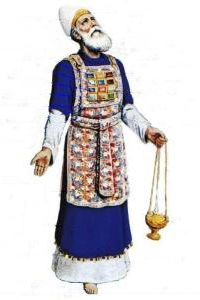
\includegraphics[width=50mm,scale=1.5]{Melchisedec.jpg}
\vspace{0.4in}

% Create a title for the document and write it in bold font
\LARGE{\textbf{\date}}
\linebreak

\vspace{0.5in}


\begin{flushleft}
\LARGE{Psalms 26-50 (Volume II)\\}\vspace{0.25in}
\LARGE{Notes, Outlines, Comments}
\end{flushleft}

% write in large letters
%\large{Free webservices and apps}

% Skip some space
\vspace{0.6in}

%\large{Documentation}
% Skip some space

\bigskip

\normalsize{Xenia, Oh.\\}
\normalsize{updated: \today}

% Skip some space
\vspace{1.3in}

\end{flushright}
% End the title page
\end{titlepage}

%\titlehttps://www.overleaf.com/project/60d732302fc633866943c9d2JE

\newpage 

\tableofcontents\hypertarget{TOC}{}
\listoffigures
\listoftables

\hyphenation{A-bim-e-lech bre-thren E-phra-im  Gib-e-o-nites Jer-u-sa-lem through-out Phil-i-stines The-o-phil-us Am-a-le-kites ven-geance Mesh-el-e-mi-ah onan-ism Phar-a-oh Py-thon thoughts grev-ous-ness Hach-a-liah adul-ter-er Shad-rach}

%\fcolorbox{black}{bone}{TEXT}
%%%%%%%%%%%%%%%%% EXTRA COLORS
%%%%%%%%%%%%%%%%% EXTRA COLORS
%%%%%%%%%%%%%%%%% EXTRA COLORS
\definecolor{champagne}{rgb}{0.97,0.91,0.81}
\definecolor{bone}{rgb}{0.89,0.85,0.79}

\definecolor{ForestGreen}{rgb}{0.00,0.29,0.098}
\definecolor{GIVING}{cmyk}{1,0.0,0.72,.1}

\definecolor{MLPE}{cmyk}{1,1,0,.45}
\definecolor{SOCCER}{cmyk}{.77, 0, .42, .49}
\definecolor{PAYBILL}{cmyk}{0,0.83,0.76,0.07}
\definecolor{SERMON}{cmyk}{.14,.9,0,.30} % aka seance \href{http://www.flatuicolorpicker.com/purple-cmyk-color-model/}{seance}
\definecolor{BIBLE}{cmyk}{0,.17,.74,.17}
\definecolor{WORKBLUE}{cmyk}{1, .5, 0, .6}
\definecolor{myOrange}{cmyk}{0, .4, .98, .03}
\definecolor{myTan}{cmyk}{0.0,.07,.17,.10}
\definecolor{myRed}{cmyk}{0,1,1,0}
\definecolor{myWhite}{cmyk}{0,0,0,0}
\definecolor{BLUESoD}{cmyk}{.97,.84,0,.04}
\definecolor{WHITE}{cmyk}{0,0,0,0}
\definecolor{OLDGOLD}{cmyk}{0.05,0.3,1.00,0}
\definecolor{CASTLETON}{cmyk}{1,0,0.31,0.66}
\definecolor{cadmiumgreen}{rgb}{0.0, 0.42, 0.24}
\definecolor{jungle}{rgb}{0.203,0.4882,0.1718}
\definecolor{MYGOLD}{rgb}{1,.84,0}

\definecolor{MYLIGHTGRAY}{rgb}{.85,.85,.85}

\definecolor{codegreen}{rgb}{0,0.6,0}
\definecolor{codegray}{rgb}{0.5,0.5,0.5}
\definecolor{codepurple}{rgb}{0.58,0,0.82}
\definecolor{backcolour}{rgb}{0.95,0.95,0.92}



\mdfdefinestyle{MyFrame}{%
    linecolor=blue,
    outerlinewidth=2pt,
    roundcorner=5pt,
    innertopmargin=\baselineskip,
    innerbottommargin=\baselineskip,
    innerrightmargin=10pt,
    innerleftmargin=10pt,
    backgroundcolor=gray!25!white}


\mdfdefinestyle{MyFrame2}{%
    linecolor=black,
    outerlinewidth=2pt,
    roundcorner=5pt,
    innertopmargin=\baselineskip,
    innerbottommargin=\baselineskip,
    innerrightmargin=10pt,
    innerleftmargin=10pt,
    backgroundcolor=yellow!25!white}



%\input{PFTTIS}
%\input{WFTTIS}
%\input{WFITV}

%
%\newpage
%\begin{figure}
%\begin{center}
%\includegraphics[scale=.7, angle=0]{05OT-Deuteronomy/References/AndrewSmithDeuteronomyTimeline.png}
%\caption[Deuteronomy Timeline by Andrew Smith]{Deuteronomy Timeline by Andrew %Smith}
%\label{fig:Deuteronomy Timeline by Andrew Smith}
%\end{center}
%\end{figure}

\newpage
\begin{figure}
\begin{center}
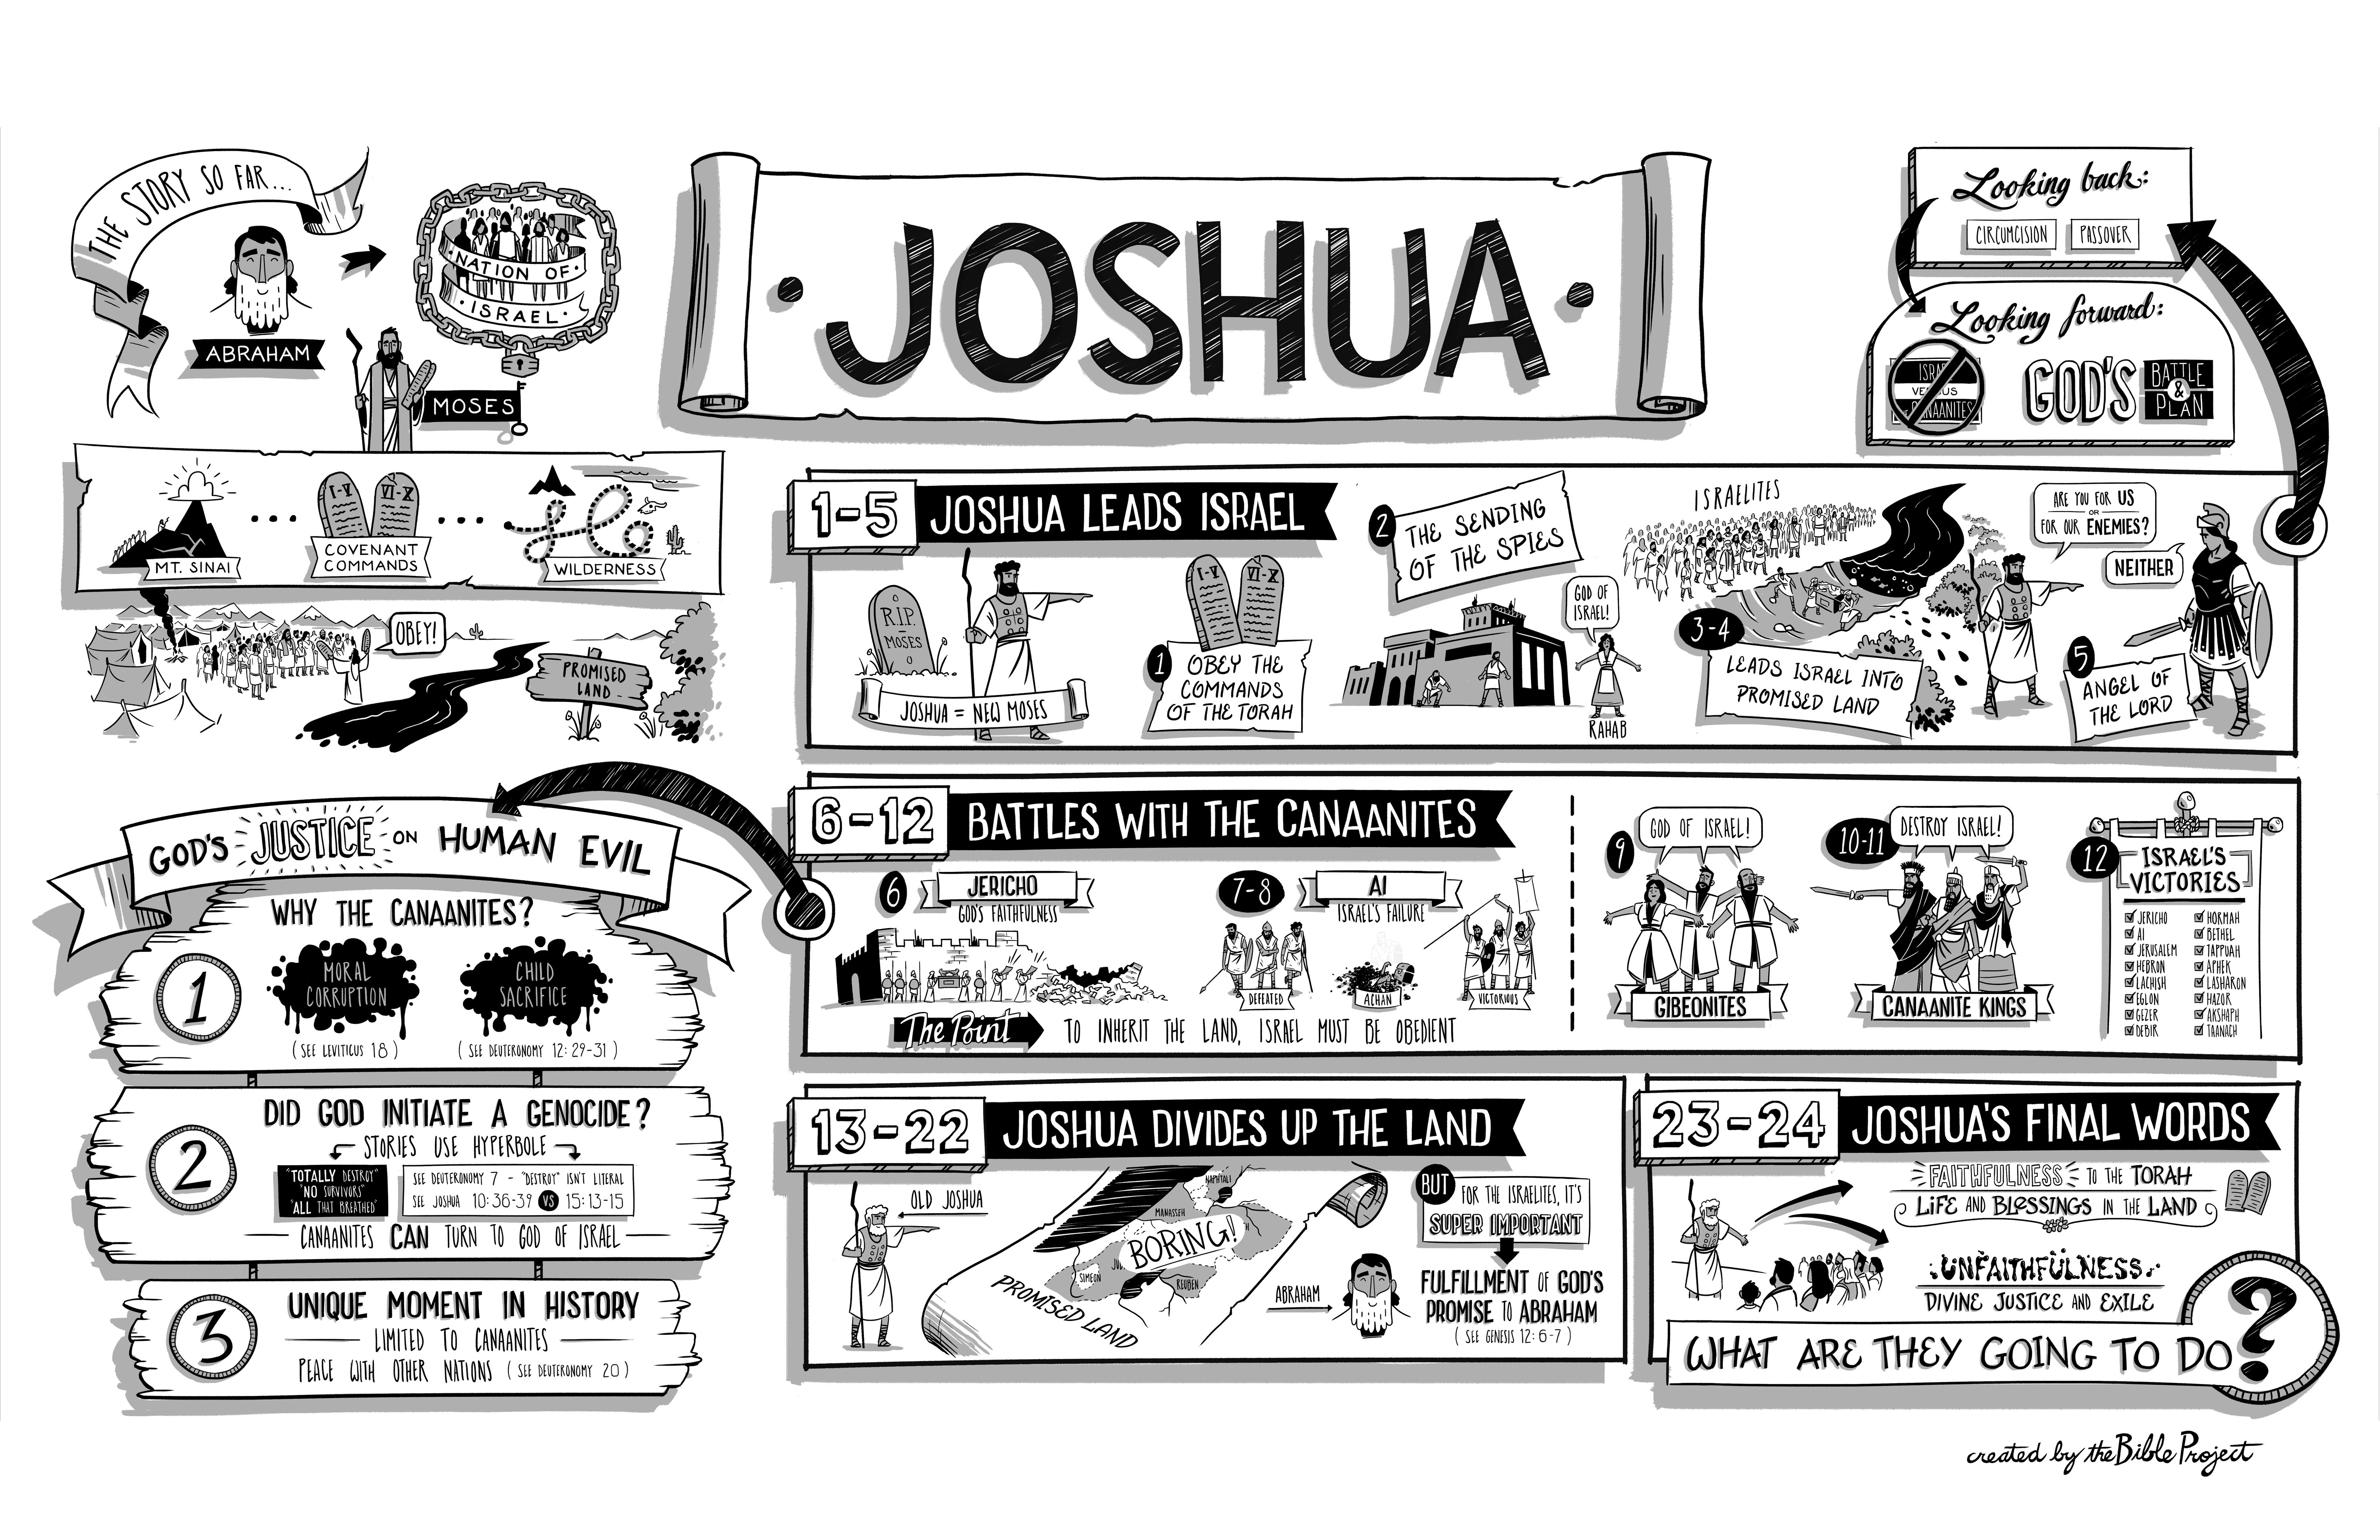
\includegraphics[scale=0.5, angle=90]{06OT-Joshua/References/1.BibleProject-Joshua.jpg}
\caption[Joshua from the Bible Project]{Joshua from the Bible Project}
\label{fig:Joshua from the Bible Project}
\end{center}
\end{figure}

\newpage
\begin{figure}
\begin{center}
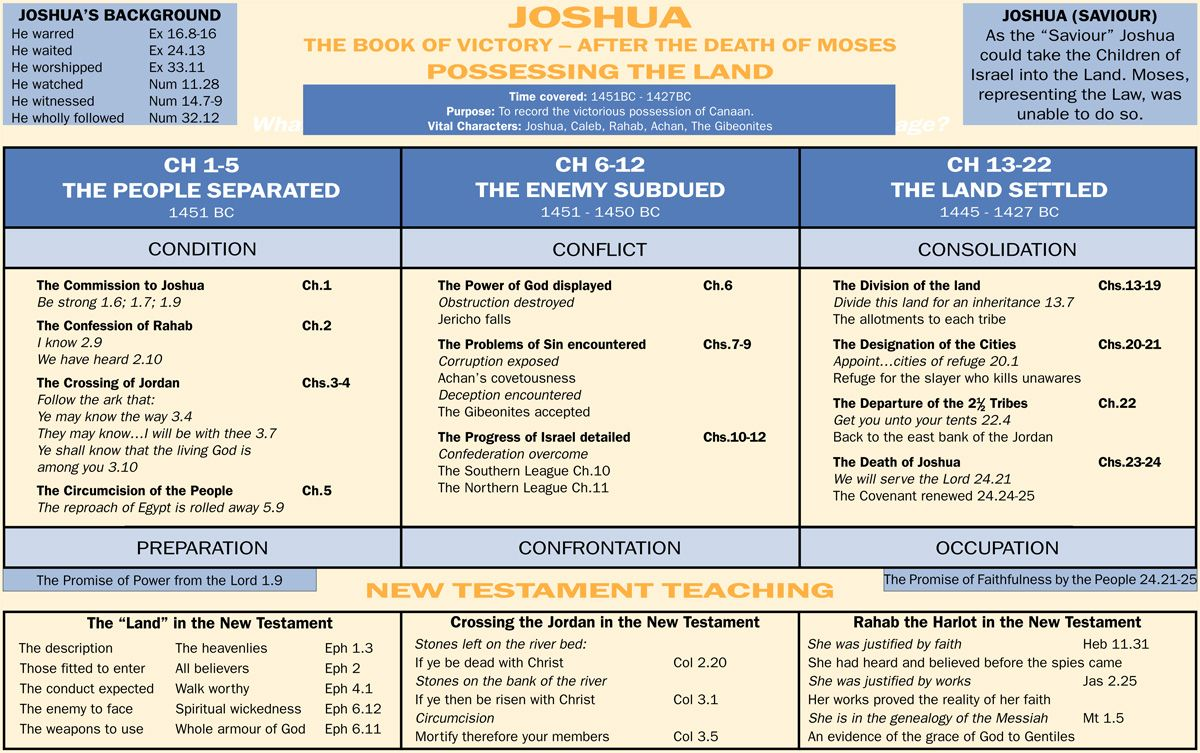
\includegraphics[scale=0.5, angle=90]{06OT-Joshua/References/2.JohnGrant-Joshua.jpg}
\caption[Joshua from John Grant]{Joshua from John Grant}
\label{fig:Joshua from John Grant}
\end{center}
\end{figure}

\newpage
\begin{figure}
\begin{center}
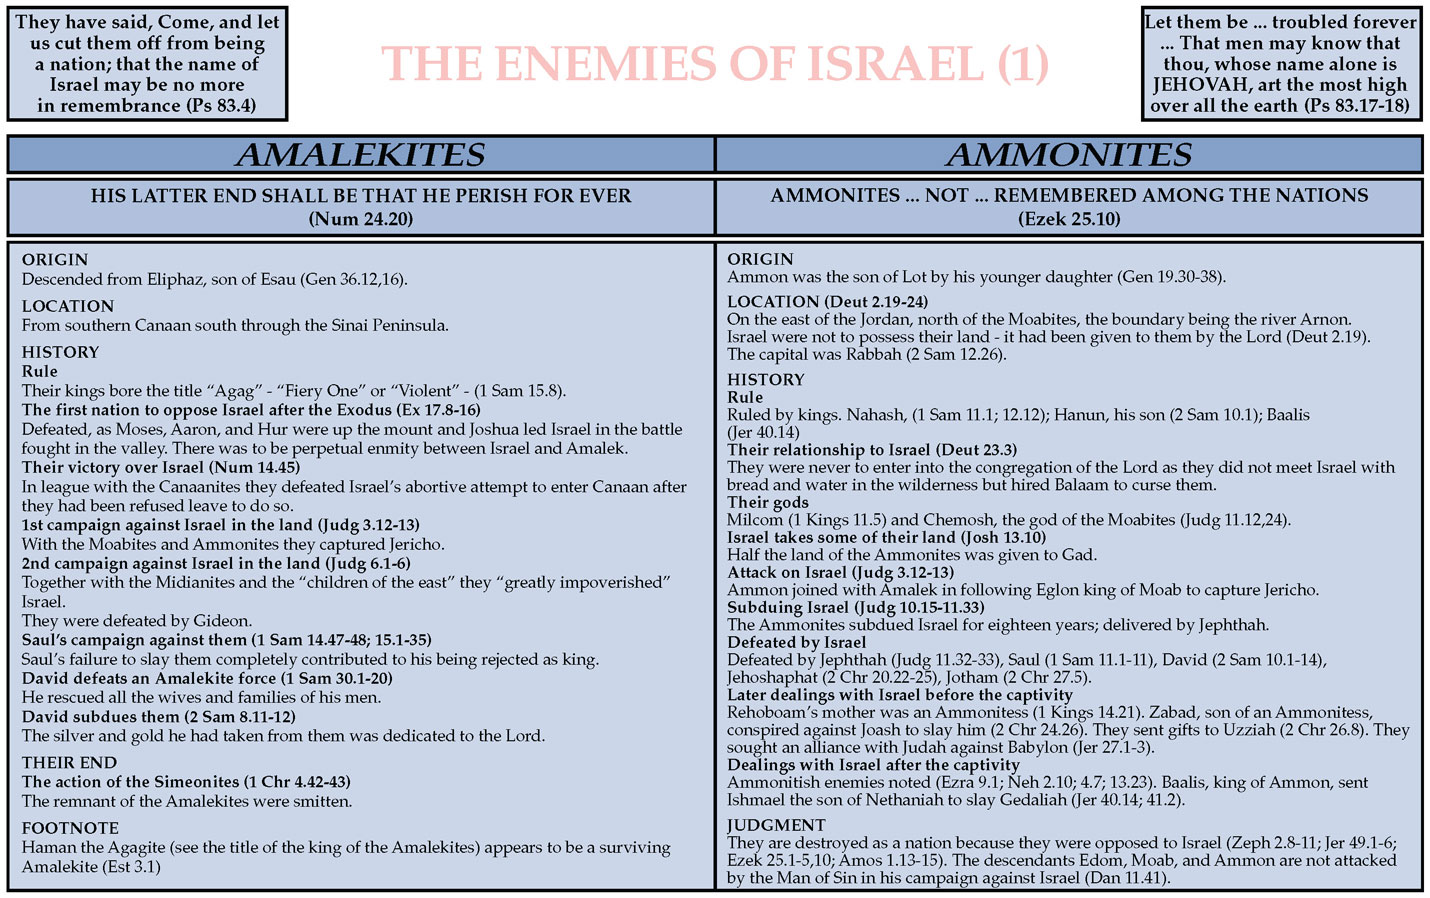
\includegraphics[scale=0.4, angle=90]{06OT-Joshua/References/3.EnemiesOfIsrael1.jpg}
\caption[Enemies of Israel 1]{Enemies of Israel 1}
\label{fig:Enemies of Israel 1}
\end{center}
\end{figure}

\newpage
\begin{figure}
\begin{center}
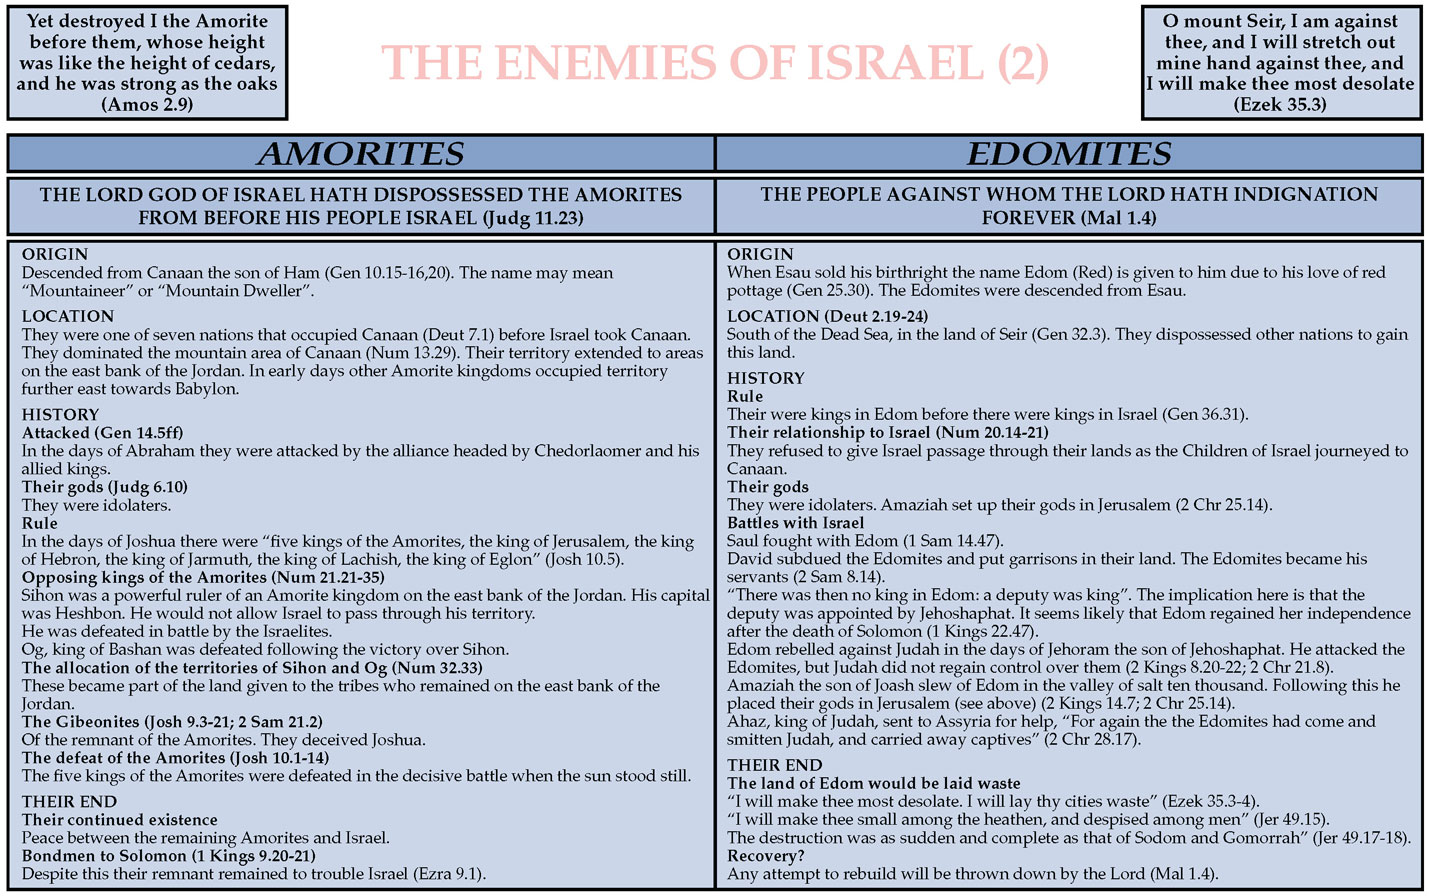
\includegraphics[scale=0.4, angle=90]{06OT-Joshua/References/4.EnemiesOfIsrael2.jpg}
\caption[Enemies of Israel 2]{Enemies of Israel 2}
\label{fig:Enemies of Israel 2}
\end{center}
\end{figure}

\newpage
\begin{figure}
\begin{center}
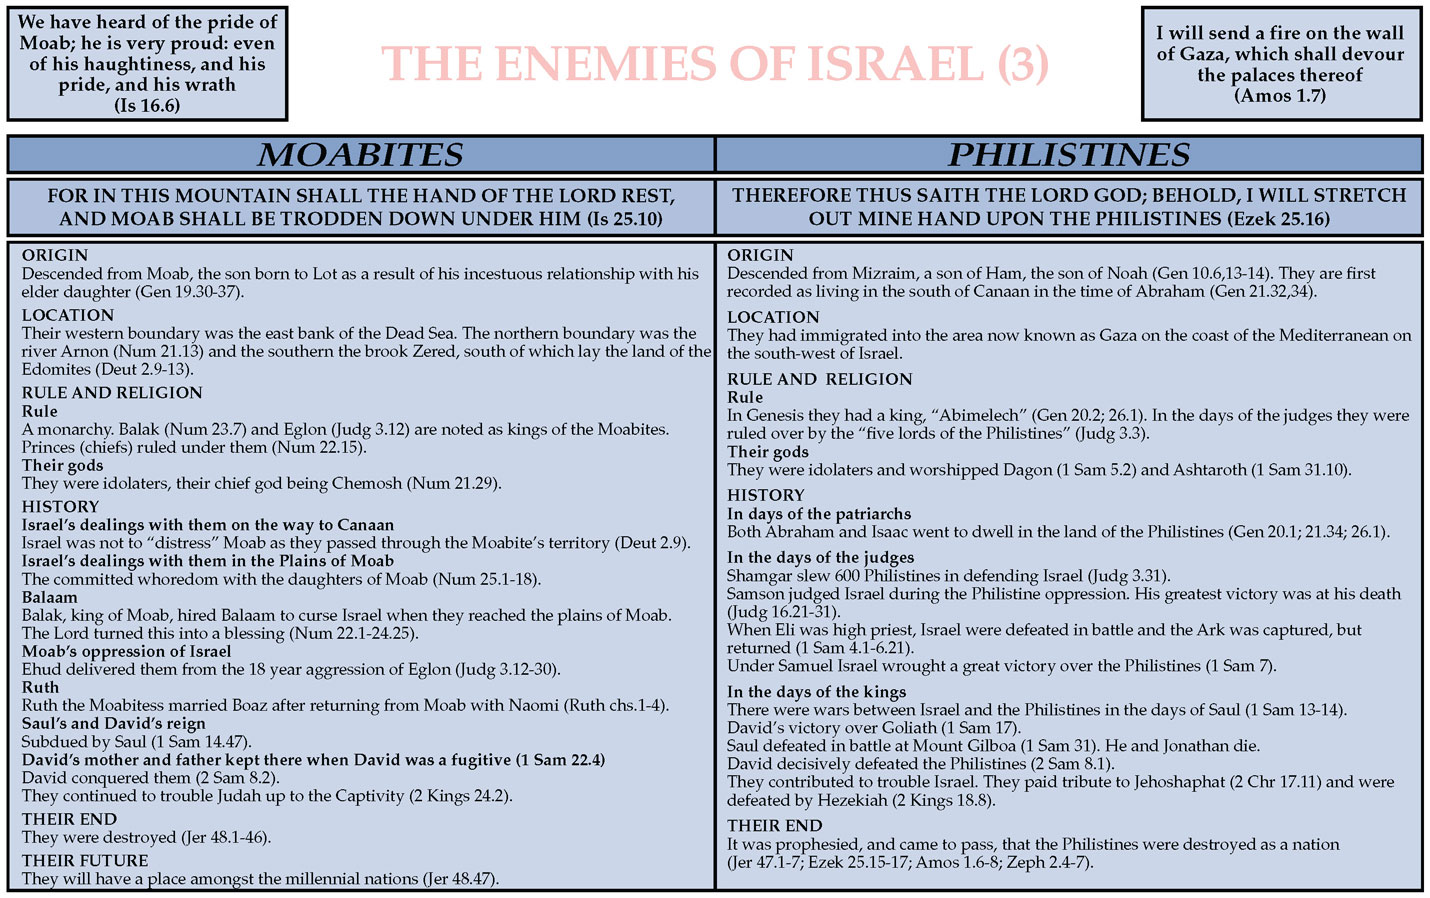
\includegraphics[scale=0.4, angle=90]{06OT-Joshua/References/5.EnemiesOfIsrael3.jpg}
\caption[Enemies of Israel 3]{Enemies of Israel 3}
\label{fig:Enemies of Israel 3}
\end{center}
\end{figure}

\newpage
\begin{figure}
\begin{center}
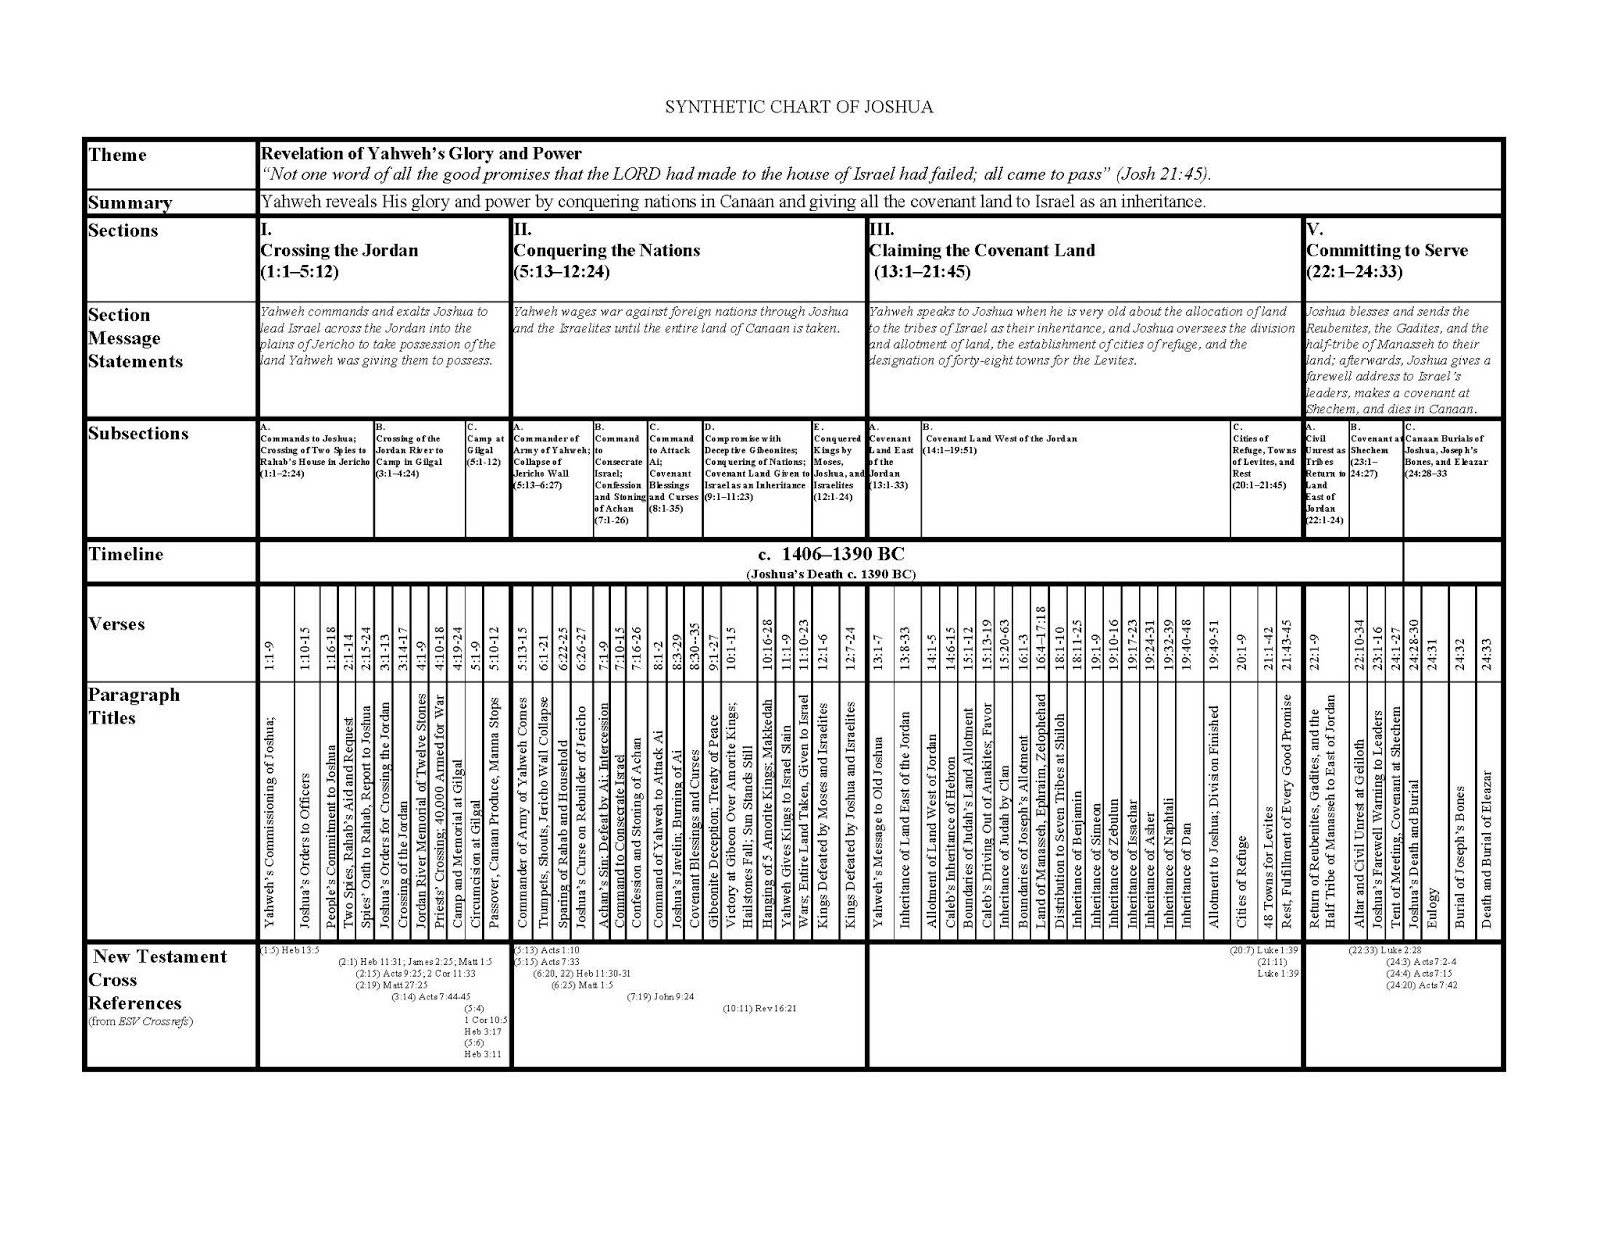
\includegraphics[scale=.4, angle=90]{06OT-Joshua/References/6.SyntheticChartofJoshua.jpg}
\caption[Synthetic Chart of Joshua]{Synthetic Chart of Joshua}
\label{fig:Synthetic Chart of Joshua}
\end{center}
\end{figure}


\newpage
\begin{figure}
\begin{center}
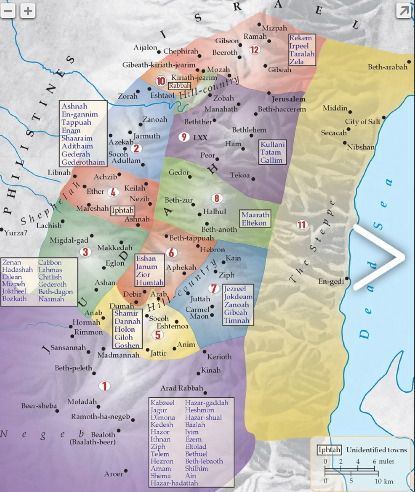
\includegraphics[scale=1, angle=0]{06OT-Joshua/References/7.WestSideOfDeadSea.jpg}
\caption[The West Side of the Dead Sea]{The West Side of the Dead Sea}
\label{fig:The West Side of the Dead Sea}
\end{center}
\end{figure}


\newpage
\begin{figure}
\begin{center}
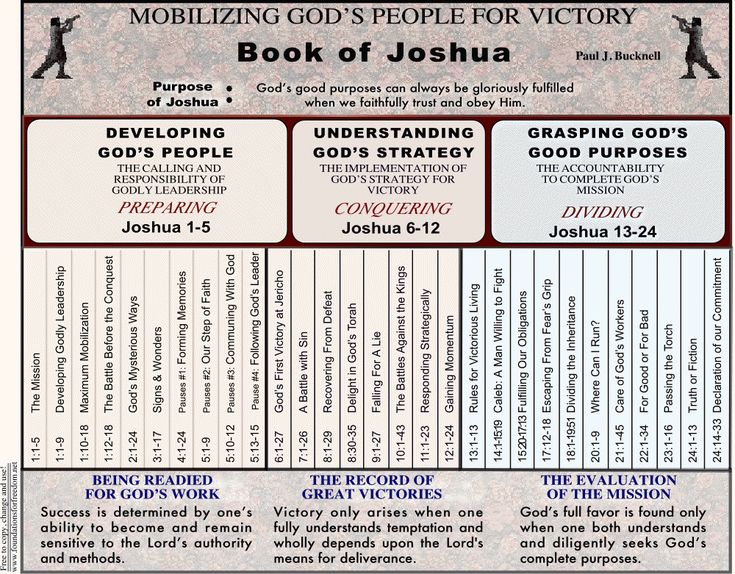
\includegraphics[scale=0.75, angle=90]{06OT-Joshua/References/8.Bucknell-Joshua.jpg}
\caption[Joshua from Bucknell]{Joshua from Bucknell}
\label{fig:Joshua from Bucknell}
\end{center}
\end{figure}


%\newpage
%\begin{figure}
%\begin{center}
%\includegraphics[scale=2, angle=90]{06OT-Joshua/References/9.Jensen-Joshua.png}
%\caption[Joshua from Jensen]{Joshua from Jensen}
%\label{fig:Joshua from Jensen}
%\end{center}
%\end{figure}


\newpage
\begin{figure}
\begin{center}
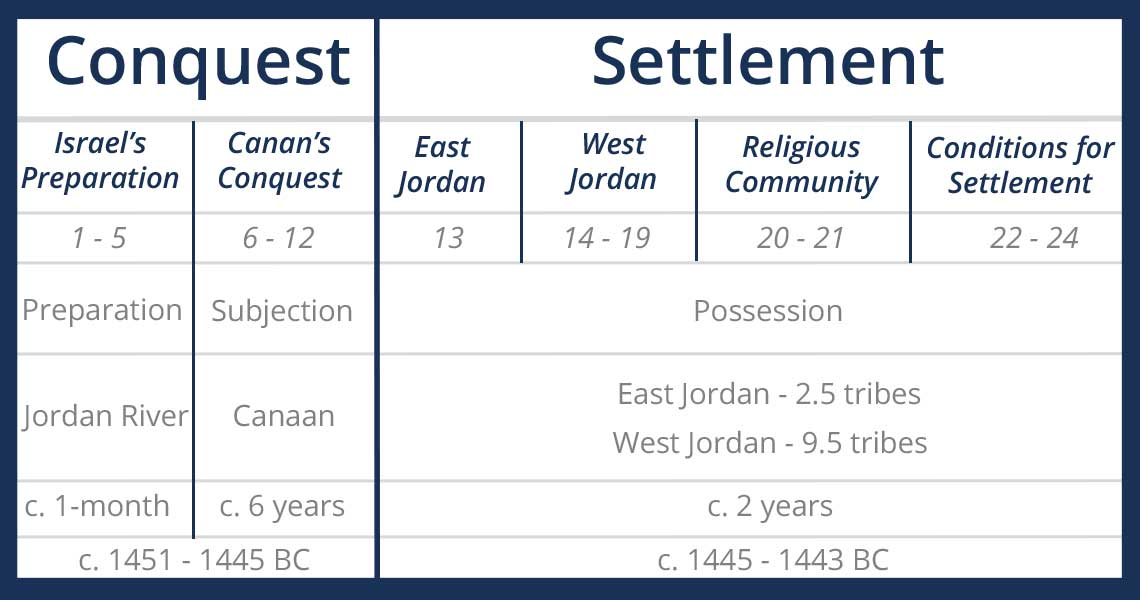
\includegraphics[scale=.5, angle=90]{06OT-Joshua/References/10.Bible-Brief-Joshua.jpg}
\caption[Bible Brief for Joshua]{Bible Brief for Joshua}
\label{fig:Bible Brief for Joshua}
\end{center}
\end{figure}

\newpage
\begin{figure}
\begin{center}
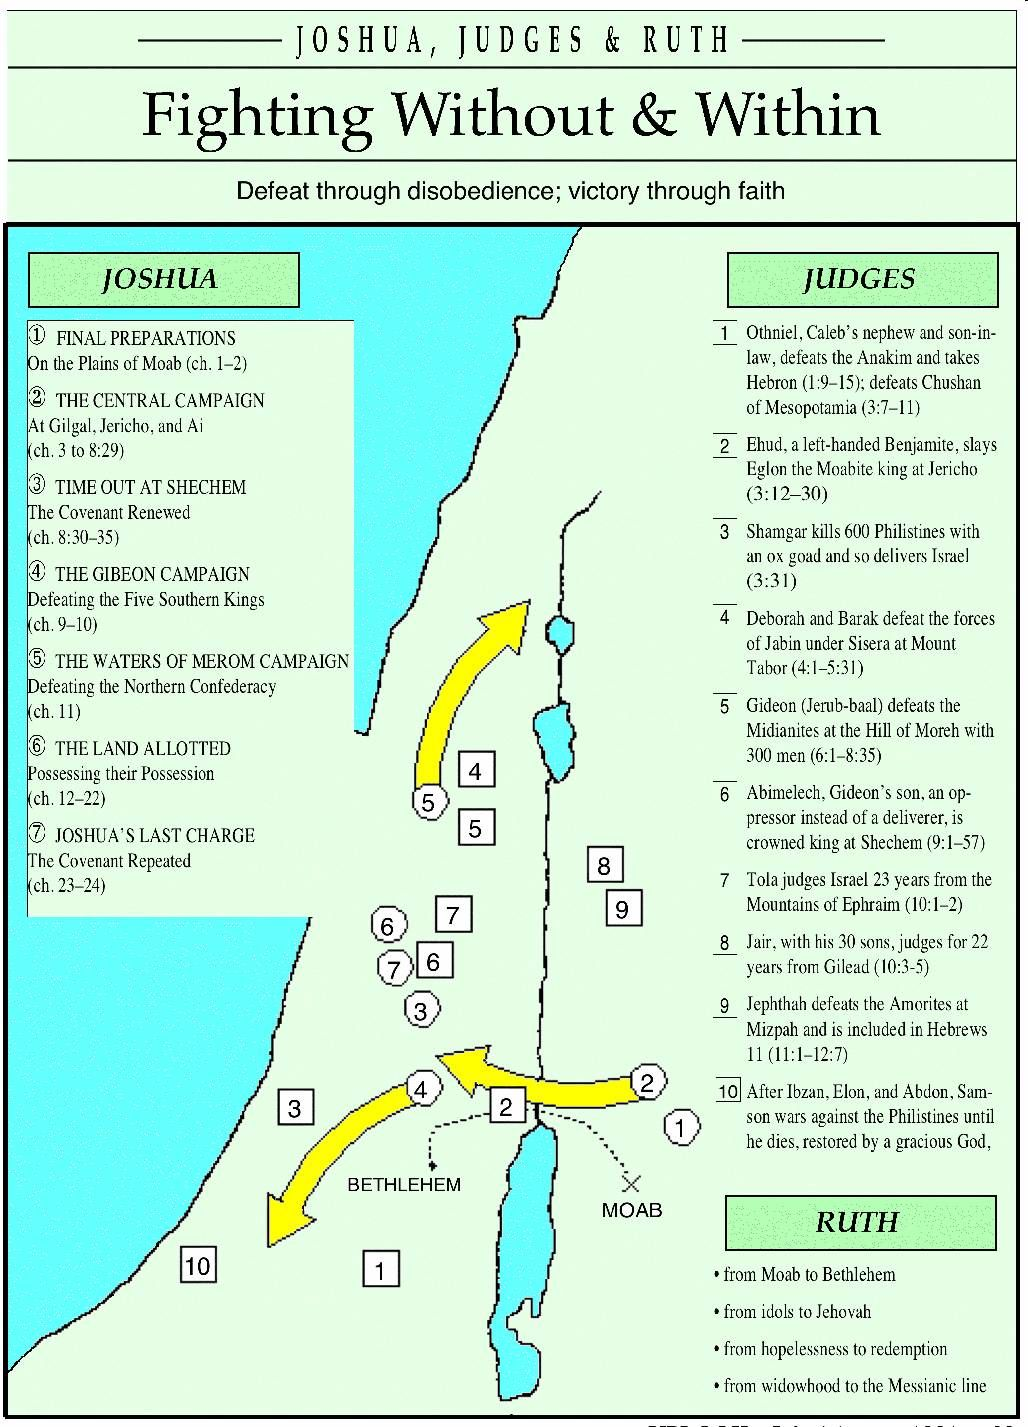
\includegraphics[scale=.5, angle=0]{06OT-Joshua/References/11.FightingInJoshuaAndJudges.jpg}
\caption[The Fighting in Joshua and Judges]{The Fighting in Joshua and Judges}
\label{fig:The Fighting in Joshua and Judges}
\end{center}
\end{figure}

\newpage
\begin{figure}
\begin{center}
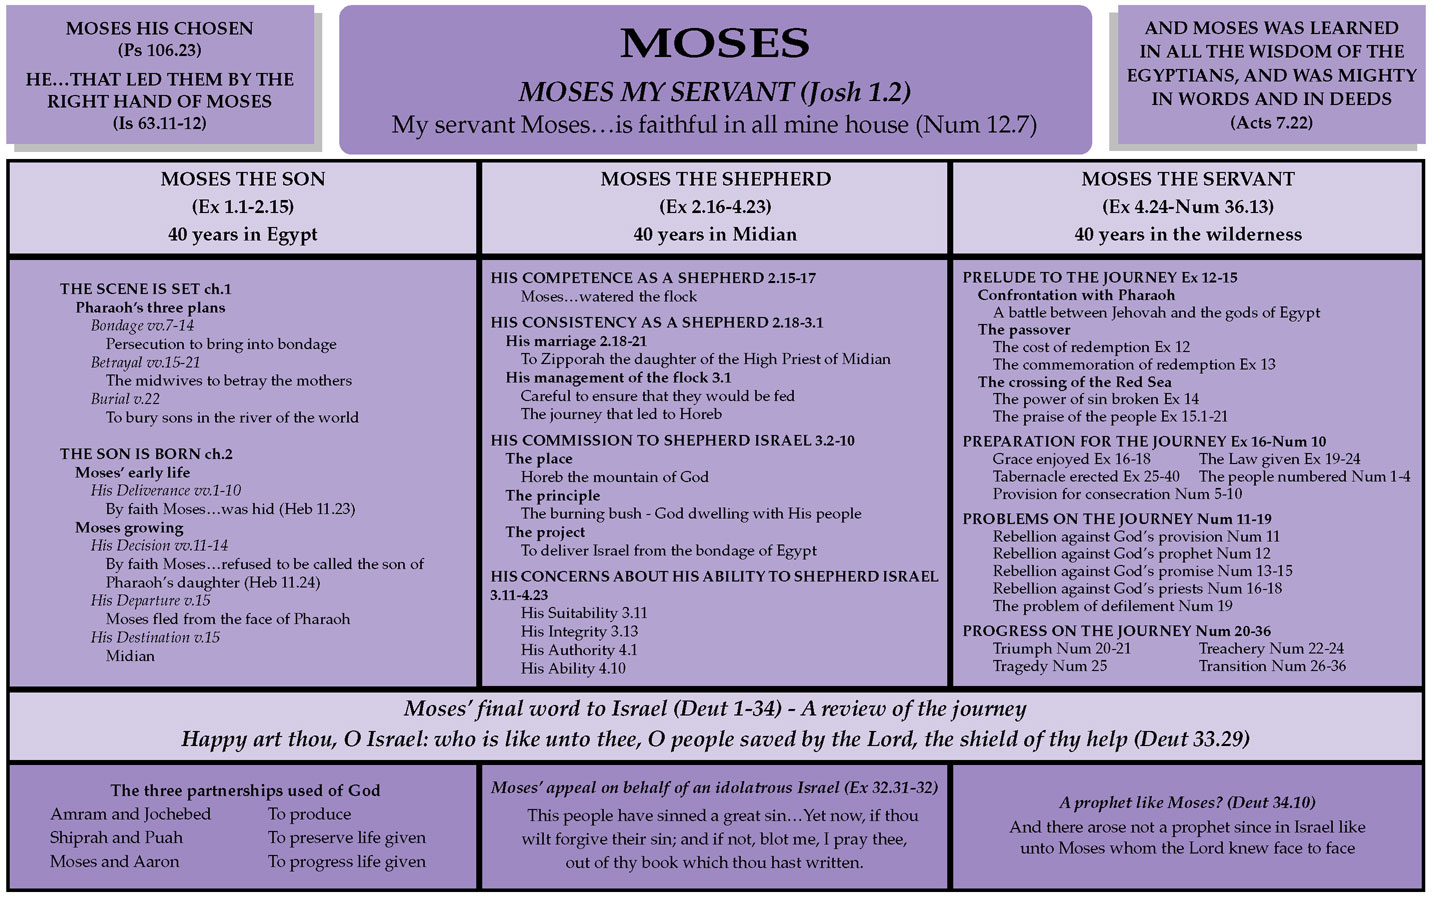
\includegraphics[scale=.4, angle=90]{06OT-Joshua/References/12.JohnGrantMoses.jpg}
\caption[Moses from John Grant]{Moses from John Grant}
\label{fig:Moses from John Grant}
\end{center}
\end{figure}







\chapter{Psalm 26}

\begin{figure}
  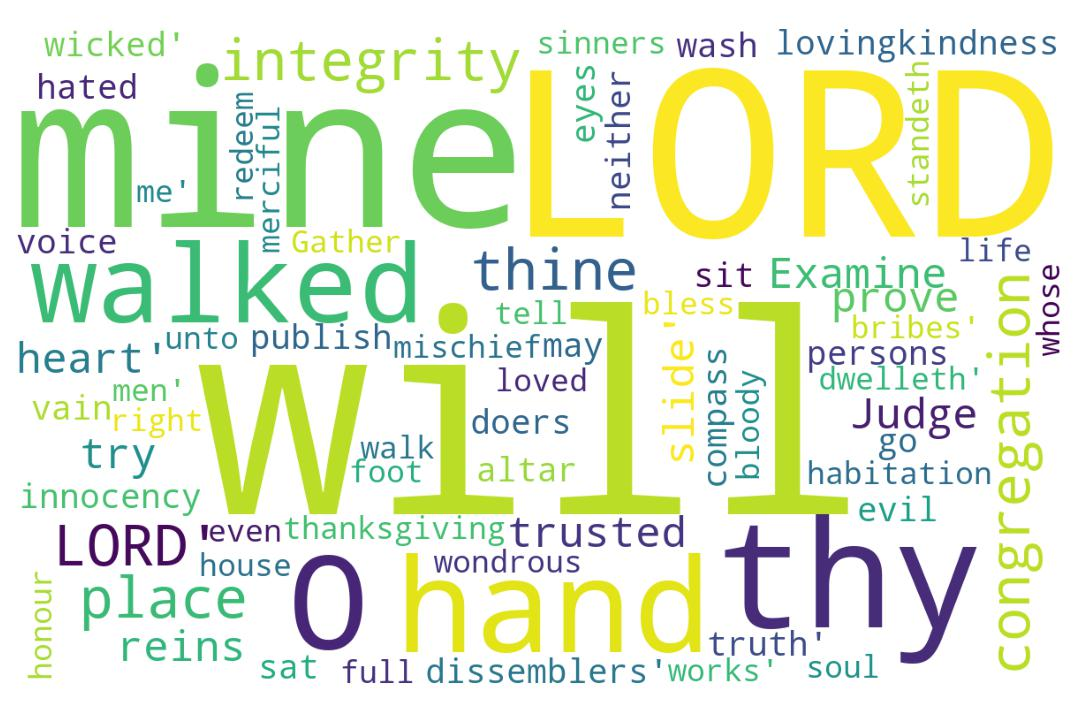
\includegraphics[width=\linewidth]{19OT-Psalms/Psalm26-WordCloud.jpg}
  \caption{Psalm 26 Word Cloud}
  \label{fig:Psalm 26 word Cloud}
\end{figure}

\marginpar{\scriptsize \centering \fcolorbox{bone}{lime}{\textbf{DAVID'S CREDIBILITY}}\\ (Psalm 26:1-12) \begin{compactenum}[I.][8]
    \item His \textbf{Purity} \index[scripture]{Psalms!Psa 026:04}\index[scripture]{Psalms!Psa 026:05}(Psa 26:4,5)
    \item His \textbf{Proof} 
    \item His \textbf{Pronouncement} 
    \item His \textbf{Performance} \index[scripture]{Psalms!Psa 026:01}\index[scripture]{Psalms!Psa 026:04}\index[scripture]{Psalms!Psa 026:05}(Psa 26:1, 4, 5)
    \item His \textbf{Proclamation}  \index[scripture]{Psalms!Psa 026:07}(Psa 26:7)
    \item His \textbf{Pleadings}  \index[scripture]{Psalms!Psa 026:09}\index[scripture]{Psalms!Psa 026:11}\index[scripture]{Psalms!Psa 026:12}(Psa 26:9,11, 12)
    \item His \textbf{Perseverance}  \index[scripture]{Psalms!Psa 026:12}(Psa 26:12)
\end{compactenum}}

\footnote{\textcolor[cmyk]{0.99998,1,0,0}{\hyperlink{TOC}{Return to end of Table of Contents.}}}\footnote{\href{https://www.audioverse.org/english/audiobibles/books/ENGKJV/O/Ps/1}{\textcolor[cmyk]{0.99998,1,0,0}{Psalms Audio}}}\textcolor[cmyk]{0.99998,1,0,0}{\emph{A Psalm} of David.}\\
\\
\textcolor[cmyk]{0.99998,1,0,0}{Judge me, O LORD; for \fcolorbox{bone}{bone}{I} have \fcolorbox{bone}{lime}{walked} in mine integrity: \fcolorbox{bone}{bone}{I} have trusted also in the LORD; \emph{therefore} \fcolorbox{bone}{bone}{I} shall not slide.}
[2] \textcolor[cmyk]{0.99998,1,0,0}{Examine me, O LORD, and prove me; try my reins and my heart.}
[3] \textcolor[cmyk]{0.99998,1,0,0}{For thy lovingkindness \emph{is} before mine eyes: and \fcolorbox{bone}{bone}{I} have walked in thy truth.}
[4] \textcolor[cmyk]{0.99998,1,0,0}{\fcolorbox{bone}{bone}{I} have \fcolorbox{bone}{lime}{not sat} with vain persons, \fcolorbox{bone}{lime}{neither will \fcolorbox{bone}{bone}{I} go} in with dissemblers.}
[5] \textcolor[cmyk]{0.99998,1,0,0}{\fcolorbox{bone}{bone}{I} have \fcolorbox{bone}{lime}{hated} the congregation of evil doers; and will not sit with the wicked.}
[6] \textcolor[cmyk]{0.99998,1,0,0}{\fcolorbox{bone}{bone}{I} will wash mine hands in innocency: so will \fcolorbox{bone}{bone}{I} compass thine altar, O LORD:}
[7] \textcolor[cmyk]{0.99998,1,0,0}{That \fcolorbox{bone}{bone}{I} may \fcolorbox{bone}{lime}{publish} with the voice of thanksgiving, and tell of all thy wondrous works.}
[8] \textcolor[cmyk]{0.99998,1,0,0}{LORD, \fcolorbox{bone}{bone}{I} have loved the habitation of thy house, and the place where thine honour dwelleth.}
[9] \textcolor[cmyk]{0.99998,1,0,0}{\fcolorbox{bone}{lime}{Gather not} my soul with sinners, nor my life with bloody men:}
[10] \textcolor[cmyk]{0.99998,1,0,0}{In whose hands \emph{is} mischief, and their right hand is full of bribes.}
[11] \textcolor[cmyk]{0.99998,1,0,0}{But as for me, \fcolorbox{bone}{bone}{I} will walk in mine integrity: \fcolorbox{bone}{lime}{redeem me}, and \fcolorbox{bone}{lime}{be merciful} unto me.}
[12] \textcolor[cmyk]{0.99998,1,0,0}{My foot \fcolorbox{bone}{lime}{standeth} in an even place: in the congregations will \fcolorbox{bone}{bone}{I} bless the LORD.}
\section{Psalm 26 Comments}

\subsection{Numeric Nuggets}
\textbf{13:} There are thirteen words in verses 2 and 13. There are 13 unique words in verses 3, 6, 10, and 12. The word ``I'' is used 13 times. The 13-letter word ``congregations'' is used in the chapter. 

\subsection{Introduction}
Compare with Psalm 1. Here David walks in integrity (Psalm 26:1), stands in an even place (Psalm 26:12), and does not sit with vain persons or evil doer (Psalm 26:4, 5).

\subsection{Psalm 26:1}
The word ``slide'' points to the word ``backslide'', which is NOT found in scripture. The words ``backslider'', ``backsliding'', and ``backslidings'' are. Forms of the word are found 13 times in Jeremiah.

\subsection{Psalm 26:12}
The word ``congreations'' is found 3 times in scripture, here and in Psalm 6:26 and 74:4.\footnote{\textbf{Psalm 68:26} - Bless ye God in the congregations, even the Lord, from the fountain of Israel.}\footnote{\textbf{Psalm 74:4} - Thine enemies roar in the midst of thy congregations; they set up their ensigns for signs.} The word ``congregation,'' on the other hand, is used 364 times, only once in the New Testament. The first occurrence is in Exodus 12:3 and the last in Acts 13:43.\footnote{\textbf{Exodus 12:3} - Speak ye unto all the congregation of Israel, saying, In the tenth day of this month they shall take to them every man a lamb, according to the house of their fathers, a lamb for an house:}\footnote{\textbf{Acts 13:43} - Now when the congregation was broken up, many of the Jews and religious proselytes followed Paul and Barnabas: who, speaking to them, persuaded them to continue in the grace of God.}
%\index[NWIV]{23!Psalms!Psa 26:1}\index[AWIP]{Judge!Psalms!Psa 26:1}\index[AWIP]{me!Psalms!Psa 26:1}\index[AWIP]{O!Psalms!Psa 26:1}\index[AWIP]{LORD!Psalms!Psa 26:1}\index[AWIP]{LORD!Psalms!Psa 26:1 (2)}\index[AWIP]{for!Psalms!Psa 26:1}\index[AWIP]{I!Psalms!Psa 26:1}\index[AWIP]{I!Psalms!Psa 26:1 (2)}\index[AWIP]{I!Psalms!Psa 26:1 (3)}\index[AWIP]{have!Psalms!Psa 26:1}\index[AWIP]{have!Psalms!Psa 26:1 (2)}\index[AWIP]{walked!Psalms!Psa 26:1}\index[AWIP]{in!Psalms!Psa 26:1}\index[AWIP]{in!Psalms!Psa 26:1 (2)}\index[AWIP]{mine!Psalms!Psa 26:1}\index[AWIP]{integrity!Psalms!Psa 26:1}\index[AWIP]{trusted!Psalms!Psa 26:1}\index[AWIP]{also!Psalms!Psa 26:1}\index[AWIP]{the!Psalms!Psa 26:1}\index[AWIP]{\emph{therefore}!Psalms!Psa 26:1}\index[AWIP]{shall!Psalms!Psa 26:1}\index[AWIP]{not!Psalms!Psa 26:1}\index[AWIP]{slide!Psalms!Psa 26:1}\index[AWIP]{\emph{therefore}!Psalms!Psa 26:1}

\index[NWIV]{13!Psalms!Psa 26:2}\index[AWIP]{Examine!Psalms!Psa 26:2}\index[AWIP]{me!Psalms!Psa 26:2}\index[AWIP]{me!Psalms!Psa 26:2 (2)}\index[AWIP]{O!Psalms!Psa 26:2}\index[AWIP]{LORD!Psalms!Psa 26:2}\index[AWIP]{and!Psalms!Psa 26:2}\index[AWIP]{and!Psalms!Psa 26:2 (2)}\index[AWIP]{prove!Psalms!Psa 26:2}\index[AWIP]{try!Psalms!Psa 26:2}\index[AWIP]{my!Psalms!Psa 26:2}\index[AWIP]{my!Psalms!Psa 26:2 (2)}\index[AWIP]{reins!Psalms!Psa 26:2}\index[AWIP]{heart!Psalms!Psa 26:2}

\index[NWIV]{14!Psalms!Psa 26:3}\index[AWIP]{For!Psalms!Psa 26:3}\index[AWIP]{thy!Psalms!Psa 26:3}\index[AWIP]{thy!Psalms!Psa 26:3 (2)}\index[AWIP]{lovingkindness!Psalms!Psa 26:3}\index[AWIP]{\emph{is}!Psalms!Psa 26:3}\index[AWIP]{before!Psalms!Psa 26:3}\index[AWIP]{mine!Psalms!Psa 26:3}\index[AWIP]{eyes!Psalms!Psa 26:3}\index[AWIP]{and!Psalms!Psa 26:3}\index[AWIP]{I!Psalms!Psa 26:3}\index[AWIP]{have!Psalms!Psa 26:3}\index[AWIP]{walked!Psalms!Psa 26:3}\index[AWIP]{in!Psalms!Psa 26:3}\index[AWIP]{truth!Psalms!Psa 26:3}\index[AWIP]{\emph{is}!Psalms!Psa 26:3}

\index[NWIV]{14!Psalms!Psa 26:4}\index[AWIP]{I!Psalms!Psa 26:4}\index[AWIP]{I!Psalms!Psa 26:4 (2)}\index[AWIP]{have!Psalms!Psa 26:4}\index[AWIP]{not!Psalms!Psa 26:4}\index[AWIP]{sat!Psalms!Psa 26:4}\index[AWIP]{with!Psalms!Psa 26:4}\index[AWIP]{with!Psalms!Psa 26:4 (2)}\index[AWIP]{vain!Psalms!Psa 26:4}\index[AWIP]{persons!Psalms!Psa 26:4}\index[AWIP]{neither!Psalms!Psa 26:4}\index[AWIP]{will!Psalms!Psa 26:4}\index[AWIP]{go!Psalms!Psa 26:4}\index[AWIP]{in!Psalms!Psa 26:4}\index[AWIP]{dissemblers!Psalms!Psa 26:4}

\index[NWIV]{15!Psalms!Psa 26:5}\index[AWIP]{I!Psalms!Psa 26:5}\index[AWIP]{have!Psalms!Psa 26:5}\index[AWIP]{hated!Psalms!Psa 26:5}\index[AWIP]{the!Psalms!Psa 26:5}\index[AWIP]{the!Psalms!Psa 26:5 (2)}\index[AWIP]{congregation!Psalms!Psa 26:5}\index[AWIP]{of!Psalms!Psa 26:5}\index[AWIP]{evil!Psalms!Psa 26:5}\index[AWIP]{doers!Psalms!Psa 26:5}\index[AWIP]{and!Psalms!Psa 26:5}\index[AWIP]{will!Psalms!Psa 26:5}\index[AWIP]{not!Psalms!Psa 26:5}\index[AWIP]{sit!Psalms!Psa 26:5}\index[AWIP]{with!Psalms!Psa 26:5}\index[AWIP]{wicked!Psalms!Psa 26:5}

\index[NWIV]{15!Psalms!Psa 26:6}\index[AWIP]{I!Psalms!Psa 26:6}\index[AWIP]{I!Psalms!Psa 26:6 (2)}\index[AWIP]{will!Psalms!Psa 26:6}\index[AWIP]{will!Psalms!Psa 26:6 (2)}\index[AWIP]{wash!Psalms!Psa 26:6}\index[AWIP]{mine!Psalms!Psa 26:6}\index[AWIP]{hands!Psalms!Psa 26:6}\index[AWIP]{in!Psalms!Psa 26:6}\index[AWIP]{innocency!Psalms!Psa 26:6}\index[AWIP]{so!Psalms!Psa 26:6}\index[AWIP]{compass!Psalms!Psa 26:6}\index[AWIP]{thine!Psalms!Psa 26:6}\index[AWIP]{altar!Psalms!Psa 26:6}\index[AWIP]{O!Psalms!Psa 26:6}\index[AWIP]{LORD!Psalms!Psa 26:6}

\index[NWIV]{16!Psalms!Psa 26:7}\index[AWIP]{That!Psalms!Psa 26:7}\index[AWIP]{I!Psalms!Psa 26:7}\index[AWIP]{may!Psalms!Psa 26:7}\index[AWIP]{publish!Psalms!Psa 26:7}\index[AWIP]{with!Psalms!Psa 26:7}\index[AWIP]{the!Psalms!Psa 26:7}\index[AWIP]{voice!Psalms!Psa 26:7}\index[AWIP]{of!Psalms!Psa 26:7}\index[AWIP]{of!Psalms!Psa 26:7 (2)}\index[AWIP]{thanksgiving!Psalms!Psa 26:7}\index[AWIP]{and!Psalms!Psa 26:7}\index[AWIP]{tell!Psalms!Psa 26:7}\index[AWIP]{all!Psalms!Psa 26:7}\index[AWIP]{thy!Psalms!Psa 26:7}\index[AWIP]{wondrous!Psalms!Psa 26:7}\index[AWIP]{works!Psalms!Psa 26:7}

\index[NWIV]{16!Psalms!Psa 26:8}\index[AWIP]{LORD!Psalms!Psa 26:8}\index[AWIP]{I!Psalms!Psa 26:8}\index[AWIP]{have!Psalms!Psa 26:8}\index[AWIP]{loved!Psalms!Psa 26:8}\index[AWIP]{the!Psalms!Psa 26:8}\index[AWIP]{the!Psalms!Psa 26:8 (2)}\index[AWIP]{habitation!Psalms!Psa 26:8}\index[AWIP]{of!Psalms!Psa 26:8}\index[AWIP]{thy!Psalms!Psa 26:8}\index[AWIP]{house!Psalms!Psa 26:8}\index[AWIP]{and!Psalms!Psa 26:8}\index[AWIP]{place!Psalms!Psa 26:8}\index[AWIP]{where!Psalms!Psa 26:8}\index[AWIP]{thine!Psalms!Psa 26:8}\index[AWIP]{honour!Psalms!Psa 26:8}\index[AWIP]{dwelleth!Psalms!Psa 26:8}

\index[NWIV]{12!Psalms!Psa 26:9}\index[AWIP]{Gather!Psalms!Psa 26:9}\index[AWIP]{not!Psalms!Psa 26:9}\index[AWIP]{my!Psalms!Psa 26:9}\index[AWIP]{my!Psalms!Psa 26:9 (2)}\index[AWIP]{soul!Psalms!Psa 26:9}\index[AWIP]{with!Psalms!Psa 26:9}\index[AWIP]{with!Psalms!Psa 26:9 (2)}\index[AWIP]{sinners!Psalms!Psa 26:9}\index[AWIP]{nor!Psalms!Psa 26:9}\index[AWIP]{life!Psalms!Psa 26:9}\index[AWIP]{bloody!Psalms!Psa 26:9}\index[AWIP]{men!Psalms!Psa 26:9}

\index[NWIV]{13!Psalms!Psa 26:10}\index[AWIP]{In!Psalms!Psa 26:10}\index[AWIP]{whose!Psalms!Psa 26:10}\index[AWIP]{hands!Psalms!Psa 26:10}\index[AWIP]{\emph{is}!Psalms!Psa 26:10}\index[AWIP]{mischief!Psalms!Psa 26:10}\index[AWIP]{and!Psalms!Psa 26:10}\index[AWIP]{their!Psalms!Psa 26:10}\index[AWIP]{right!Psalms!Psa 26:10}\index[AWIP]{hand!Psalms!Psa 26:10}\index[AWIP]{is!Psalms!Psa 26:10}\index[AWIP]{full!Psalms!Psa 26:10}\index[AWIP]{of!Psalms!Psa 26:10}\index[AWIP]{bribes!Psalms!Psa 26:10}\index[AWIP]{\emph{is}!Psalms!Psa 26:10}

\index[NWIV]{17!Psalms!Psa 26:11}\index[AWIP]{But!Psalms!Psa 26:11}\index[AWIP]{as!Psalms!Psa 26:11}\index[AWIP]{for!Psalms!Psa 26:11}\index[AWIP]{me!Psalms!Psa 26:11}\index[AWIP]{me!Psalms!Psa 26:11 (2)}\index[AWIP]{me!Psalms!Psa 26:11 (3)}\index[AWIP]{I!Psalms!Psa 26:11}\index[AWIP]{will!Psalms!Psa 26:11}\index[AWIP]{walk!Psalms!Psa 26:11}\index[AWIP]{in!Psalms!Psa 26:11}\index[AWIP]{mine!Psalms!Psa 26:11}\index[AWIP]{integrity!Psalms!Psa 26:11}\index[AWIP]{redeem!Psalms!Psa 26:11}\index[AWIP]{and!Psalms!Psa 26:11}\index[AWIP]{be!Psalms!Psa 26:11}\index[AWIP]{merciful!Psalms!Psa 26:11}\index[AWIP]{unto!Psalms!Psa 26:11}

\index[NWIV]{15!Psalms!Psa 26:12}\index[AWIP]{My!Psalms!Psa 26:12}\index[AWIP]{foot!Psalms!Psa 26:12}\index[AWIP]{standeth!Psalms!Psa 26:12}\index[AWIP]{in!Psalms!Psa 26:12}\index[AWIP]{in!Psalms!Psa 26:12 (2)}\index[AWIP]{an!Psalms!Psa 26:12}\index[AWIP]{even!Psalms!Psa 26:12}\index[AWIP]{place!Psalms!Psa 26:12}\index[AWIP]{the!Psalms!Psa 26:12}\index[AWIP]{the!Psalms!Psa 26:12 (2)}\index[AWIP]{congregations!Psalms!Psa 26:12}\index[AWIP]{will!Psalms!Psa 26:12}\index[AWIP]{I!Psalms!Psa 26:12}\index[AWIP]{bless!Psalms!Psa 26:12}\index[AWIP]{LORD!Psalms!Psa 26:12}


\section{Psalm 26 Outlines}

\subsection{My Outlines}

\subsubsection{David's Credibility}
\textbf{Introduction:} Psalm 26:
\index[speaker]{Keith Anthony!Psalm 026 (David's Credibility)}
\index[series]{Psalms (Keith Anthony)!Psalm 026 (David's Credibility)}
\index[date]{2016/07/01!Psalm 026 (David's Credibility) (Keith Anthony)}
\begin{compactenum}[I.]
    \item His \textbf{Purity} \index[scripture]{Psalms!Psa 026:04}\index[scripture]{Psalms!Psa 026:05}(Psa 26:4,5)
    \item His \textbf{Proof} 
    \item His \textbf{Pronouncement} 
    \item His \textbf{Performance} \index[scripture]{Psalms!Psa 026:01}\index[scripture]{Psalms!Psa 026:04}\index[scripture]{Psalms!Psa 026:05}(Psa 26:1, 4, 5)
    \item His \textbf{Proclamation}  \index[scripture]{Psalms!Psa 026:07}(Psa 26:7)
    \item His \textbf{Pleadings}  \index[scripture]{Psalms!Psa 026:09}\index[scripture]{Psalms!Psa 026:11}\index[scripture]{Psalms!Psa 026:12}(Psa 26:9,11, 12)
    \item His \textbf{Perseverance}  \index[scripture]{Psalms!Psa 026:12}(Psa 26:12)
\end{compactenum}


\subsection{Outlines from Others}

\subsubsection{Search Me, Oh God}
\index[speaker]{John Phillips!Psalm 026 (Search Me, Oh God)}
\index[series]{Psalms (John Phillips)!Psalm 026 (Search Me, Oh God)}
\index[date]{2016/07/01!Psalm 026 (Search Me, Oh God) (John Phillips)}
\begin{compactenum}[I.]
    \item \textbf{A Divinely Open Life} (Psalm 26:1-2)\footnote{John Philips, Exploring the Psalms, Volume 1.\cite{Phillips2001ExploringPsalms1}}
    \item \textbf{A Divinely Obedient Life} (Psalm 26:3)
    \item \textbf{A Divinely Overcoming Life} (Psalm 26:4-6) 
    \begin{compactenum}[A.]
        \item The Principle of Separation (Psalm 26:4-5)
        \item The Principle of Sanctification (Psalm 26:6)
    \end{compactenum}
    \item \textbf{A Divinely Overflowing Life} (Psalm 26:7-8) \emph{(in the direction of)}
    \begin{compactenum}[A.]
        \item Praising the Lord (Psalm 26:7a)
        \item Preaching the Lord (Psalm 26:7b)
        \item Pursuing the Lord (Psalm 26:8)
    \end{compactenum}
    \item \textbf{A Divinely Obstructed Life} (Psalm 26:9-10)
    \item \textbf{A Divinely Ordered Life} (Psalm 26:11-12)
\end{compactenum}



%\section{Psalm 26 Statistics}

%%%%%%%%%%%%%%%%%%%%%%%%%%%
%%%%%Word Statistics
%%%%%%%%%%%%%%%%%%%%%%%%%%%


\normalsize



\subsection{Chapter Word Statistics}


%%%%%%%%%%
%%%%%%%%%%
 
\begin{center}
\begin{longtable}{l|c|c|c|c}
\caption[Stats for Psalm 26]{Stats for Psalm 26} \label{table:Stats for Psalm 26} \\ 
\hline \multicolumn{1}{|c|}{\textbf{Verse(s)}} & \multicolumn{1}{|c|}{\textbf{Count}} & \multicolumn{1}{|c|}{\textbf{Unique}} & \multicolumn{1}{|c|}{\textbf{Italics}} & \multicolumn{1}{|c|}{\textbf{Uniq Italic}}  \\ \hline 
\endfirsthead
 
\multicolumn{5}{c}
{{\bfseries \tablename\ \thetable{} -- continued from previous page}} \\  
\hline \multicolumn{1}{|c|}{\textbf{Verse(s)}} & \multicolumn{1}{|c|}{\textbf{Count}} & \multicolumn{1}{|c|}{\textbf{Unique}} & \multicolumn{1}{|c|}{\textbf{Italics}} & \multicolumn{1}{|c|}{\textbf{Uniq Italic}}  \\ \hline 
\endhead
 
\hline \multicolumn{5}{|r|}{{Continued if needed}} \\ \hline
\endfoot 
1 & 23 & 18 & 1 & 1\\ \hline
2 & 13 & 10 & 0 & 0\\ \hline
3 & 14 & 13 & 1 & 1\\ \hline
4 & 14 & 12 & 0 & 0\\ \hline
5 & 15 & 14 & 0 & 0\\ \hline
6 & 15 & 13 & 0 & 0\\ \hline
7 & 16 & 15 & 0 & 0\\ \hline
8 & 16 & 15 & 0 & 0\\ \hline
9 & 12 & 10 & 0 & 0\\ \hline
10 & 13 & 13 & 1 & 1\\ \hline
11 & 17 & 15 & 0 & 0\\ \hline
12 & 15 & 13 & 0 & 0\\ \hline
\hline \hline
Total & 183 & 100 & 3 & 2



\end{longtable}
\end{center}

%%%%%%%%%%
%%%%%%%%%%
 
\subsection{Words by Frequency}

\begin{center}
\begin{longtable}{l|r}
\caption[Word Frequencies in Psalm 26]{Word Frequencies in Psalm 26} \label{table:WordsIn-Psalm-26} \\ 
\hline \multicolumn{1}{|c|}{\textbf{Word}} & \multicolumn{1}{c|}{\textbf{Frequency}} \\ \hline 
\endfirsthead
 
\multicolumn{2}{c}
{{\bfseries \tablename\ \thetable{} -- continued from previous page}} \\ 
\hline \multicolumn{1}{|c|}{\textbf{Word}} & \multicolumn{1}{c|}{\textbf{Frequency}} \\ \hline 
\endhead
 
\hline \multicolumn{2}{|r|}{{Continued if needed}} \\ \hline
\endfoot
 
\hline \hline
\endlastfoot
I & 13 \\ \hline
in & 8 \\ \hline
the & 8 \\ \hline
and & 8 \\ \hline
me & 6 \\ \hline
LORD & 6 \\ \hline
have & 6 \\ \hline
with & 6 \\ \hline
will & 6 \\ \hline
of & 5 \\ \hline
mine & 4 \\ \hline
not & 4 \\ \hline
my & 4 \\ \hline
thy & 4 \\ \hline
O & 3 \\ \hline
for & 2 \\ \hline
walked & 2 \\ \hline
integrity & 2 \\ \hline
\emph{is} & 2 \\ \hline
hands & 2 \\ \hline
thine & 2 \\ \hline
place & 2 \\ \hline
Judge & 1 \\ \hline
trusted & 1 \\ \hline
also & 1 \\ \hline
\emph{therefore} & 1 \\ \hline
shall & 1 \\ \hline
slide & 1 \\ \hline
Examine & 1 \\ \hline
prove & 1 \\ \hline
try & 1 \\ \hline
reins & 1 \\ \hline
heart & 1 \\ \hline
For & 1 \\ \hline
lovingkindness & 1 \\ \hline
before & 1 \\ \hline
eyes & 1 \\ \hline
truth & 1 \\ \hline
sat & 1 \\ \hline
vain & 1 \\ \hline
persons & 1 \\ \hline
neither & 1 \\ \hline
go & 1 \\ \hline
dissemblers & 1 \\ \hline
hated & 1 \\ \hline
congregation & 1 \\ \hline
evil & 1 \\ \hline
doers & 1 \\ \hline
sit & 1 \\ \hline
wicked & 1 \\ \hline
wash & 1 \\ \hline
innocency & 1 \\ \hline
so & 1 \\ \hline
compass & 1 \\ \hline
altar & 1 \\ \hline
That & 1 \\ \hline
may & 1 \\ \hline
publish & 1 \\ \hline
voice & 1 \\ \hline
thanksgiving & 1 \\ \hline
tell & 1 \\ \hline
all & 1 \\ \hline
wondrous & 1 \\ \hline
works & 1 \\ \hline
loved & 1 \\ \hline
habitation & 1 \\ \hline
house & 1 \\ \hline
where & 1 \\ \hline
honour & 1 \\ \hline
dwelleth & 1 \\ \hline
Gather & 1 \\ \hline
soul & 1 \\ \hline
sinners & 1 \\ \hline
nor & 1 \\ \hline
life & 1 \\ \hline
bloody & 1 \\ \hline
men & 1 \\ \hline
In & 1 \\ \hline
whose & 1 \\ \hline
mischief & 1 \\ \hline
their & 1 \\ \hline
right & 1 \\ \hline
hand & 1 \\ \hline
is & 1 \\ \hline
full & 1 \\ \hline
bribes & 1 \\ \hline
But & 1 \\ \hline
as & 1 \\ \hline
walk & 1 \\ \hline
redeem & 1 \\ \hline
be & 1 \\ \hline
merciful & 1 \\ \hline
unto & 1 \\ \hline
My & 1 \\ \hline
foot & 1 \\ \hline
standeth & 1 \\ \hline
an & 1 \\ \hline
even & 1 \\ \hline
congregations & 1 \\ \hline
bless & 1 \\ \hline
\end{longtable}
\end{center}



\normalsize



\subsection{Words Alphabetically}

\begin{center}
\begin{longtable}{l|r}
\caption[Word Alphabetically in Psalm 26]{Word Alphabetically in Psalm 26} \label{table:WordsIn-Psalm-26} \\ 
\hline \multicolumn{1}{|c|}{\textbf{Word}} & \multicolumn{1}{c|}{\textbf{Frequency}} \\ \hline 
\endfirsthead
 
\multicolumn{2}{c}
{{\bfseries \tablename\ \thetable{} -- continued from previous page}} \\ 
\hline \multicolumn{1}{|c|}{\textbf{Word}} & \multicolumn{1}{c|}{\textbf{Frequency}} \\ \hline 
\endhead
 
\hline \multicolumn{2}{|r|}{{Continued if needed}} \\ \hline
\endfoot
 
\hline \hline
\endlastfoot
But & 1 \\ \hline
Examine & 1 \\ \hline
For & 1 \\ \hline
Gather & 1 \\ \hline
I & 13 \\ \hline
In & 1 \\ \hline
Judge & 1 \\ \hline
LORD & 6 \\ \hline
My & 1 \\ \hline
O & 3 \\ \hline
That & 1 \\ \hline
\emph{is} & 2 \\ \hline
\emph{therefore} & 1 \\ \hline
all & 1 \\ \hline
also & 1 \\ \hline
altar & 1 \\ \hline
an & 1 \\ \hline
and & 8 \\ \hline
as & 1 \\ \hline
be & 1 \\ \hline
before & 1 \\ \hline
bless & 1 \\ \hline
bloody & 1 \\ \hline
bribes & 1 \\ \hline
compass & 1 \\ \hline
congregation & 1 \\ \hline
congregations & 1 \\ \hline
dissemblers & 1 \\ \hline
doers & 1 \\ \hline
dwelleth & 1 \\ \hline
even & 1 \\ \hline
evil & 1 \\ \hline
eyes & 1 \\ \hline
foot & 1 \\ \hline
for & 2 \\ \hline
full & 1 \\ \hline
go & 1 \\ \hline
habitation & 1 \\ \hline
hand & 1 \\ \hline
hands & 2 \\ \hline
hated & 1 \\ \hline
have & 6 \\ \hline
heart & 1 \\ \hline
honour & 1 \\ \hline
house & 1 \\ \hline
in & 8 \\ \hline
innocency & 1 \\ \hline
integrity & 2 \\ \hline
is & 1 \\ \hline
life & 1 \\ \hline
loved & 1 \\ \hline
lovingkindness & 1 \\ \hline
may & 1 \\ \hline
me & 6 \\ \hline
men & 1 \\ \hline
merciful & 1 \\ \hline
mine & 4 \\ \hline
mischief & 1 \\ \hline
my & 4 \\ \hline
neither & 1 \\ \hline
nor & 1 \\ \hline
not & 4 \\ \hline
of & 5 \\ \hline
persons & 1 \\ \hline
place & 2 \\ \hline
prove & 1 \\ \hline
publish & 1 \\ \hline
redeem & 1 \\ \hline
reins & 1 \\ \hline
right & 1 \\ \hline
sat & 1 \\ \hline
shall & 1 \\ \hline
sinners & 1 \\ \hline
sit & 1 \\ \hline
slide & 1 \\ \hline
so & 1 \\ \hline
soul & 1 \\ \hline
standeth & 1 \\ \hline
tell & 1 \\ \hline
thanksgiving & 1 \\ \hline
the & 8 \\ \hline
their & 1 \\ \hline
thine & 2 \\ \hline
thy & 4 \\ \hline
trusted & 1 \\ \hline
truth & 1 \\ \hline
try & 1 \\ \hline
unto & 1 \\ \hline
vain & 1 \\ \hline
voice & 1 \\ \hline
walk & 1 \\ \hline
walked & 2 \\ \hline
wash & 1 \\ \hline
where & 1 \\ \hline
whose & 1 \\ \hline
wicked & 1 \\ \hline
will & 6 \\ \hline
with & 6 \\ \hline
wondrous & 1 \\ \hline
works & 1 \\ \hline
\end{longtable}
\end{center}



\normalsize



\subsection{Word Lengths in Chapter}
\normalsize
\begin{longtable}{l|p{3.75in}}
\caption[Words by Length in Psalm 26]{Words by Length in Psalm 26} \label{table:WordsIn-Psalm-26} \\ 
\hline \multicolumn{1}{|c|}{\textbf{Length}} & \multicolumn{1}{c|}{\textbf{Words}} \\ \hline 
\endfirsthead
 
\multicolumn{2}{c}
{{\bfseries \tablename\ \thetable{} -- continued from previous page}} \\ 
\hline \multicolumn{1}{|c|}{\textbf{Length}} & \multicolumn{1}{c|}{\textbf{Words}} \\ \hline 
\endhead
 
\hline \multicolumn{2}{|r|}{{Continued if needed}} \\ \hline
\endfoot
 
\hline \hline
\endlastfoot
1 & O, I \\ \hline
2 & me, in, my, \emph{is}, go, of, so, In, is, as, be, My, an \\ \hline
3 & for, the, not, and, try, For, thy, sat, sit, may, all, nor, men, But \\ \hline
4 & LORD, have, mine, also, eyes, with, vain, will, evil, wash, That, tell, soul, life, hand, full, walk, unto, foot, even \\ \hline
5 & Judge, shall, slide, prove, reins, heart, truth, hated, doers, hands, thine, altar, voice, works, loved, house, place, where, whose, their, right, bless \\ \hline
6 & walked, before, wicked, honour, Gather, bloody, bribes, redeem \\ \hline
7 & trusted, Examine, persons, neither, compass, publish, sinners \\ \hline
8 & wondrous, dwelleth, mischief, merciful, standeth \\ \hline
9 & integrity, \emph{therefore}, innocency \\ \hline
10 & habitation \\ \hline
11 & dissemblers \\ \hline
12 & congregation, thanksgiving \\ \hline
13 & congregations \\ \hline
14 & lovingkindness \\ \hline
\end{longtable}






%%%%%%%%%%
%%%%%%%%%%
 



%%%%%%%%%%
%%%%%%%%%%
\subsection{Verses with 13 Words in Chapter}
\normalsize
\begin{longtable}{l|p{3.75in}}
\caption[Verses with 13 Words  in Psalm 26]{Verses with 13 Words  in Psalm 26} \label{table:Verses with 13 Words in-Psalm-26} \\ 
\hline \multicolumn{1}{|c|}{\textbf{Reference}} & \multicolumn{1}{c|}{\textbf{Verse}} \\ \hline 
\endfirsthead
 
\multicolumn{2}{c}
{{\bfseries \tablename\ \thetable{} -- continued from previous page}} \\ 
\hline \multicolumn{1}{|c|}{\textbf{Reference}} & \multicolumn{1}{c|}{\textbf{Verse}} \\ \hline 
\endhead
 
\hline \multicolumn{2}{|r|}{{Continued if needed}} \\ \hline
\endfoot
 
\hline \hline
\endlastfoot
Psalms 026:2 & Examine me, O LORD, and prove me; try my reins and my heart. \\ \hline
Psalms 026:10 & In whose hands \emph{is} mischief, and their right hand is full of bribes. \\ \hline
\end{longtable}






%%%%%%%%%%
%%%%%%%%%%
 
\subsection{Psalm 26 Repeated Phrases}


%%%%%%%%%%
%%%%%%%%%%
\normalsize
 
\begin{center}
\begin{longtable}{|p{3.0in}|p{0.5in}|}
\caption[Psalm2 6 Repeated Phrases]{Psalm 26 Repeated Phrases}\label{table:Repeated Phrases Psalm 26} \\
\hline \multicolumn{1}{|c|}{\textbf{Phrase}} & \multicolumn{1}{c|}{\textbf{Frequency}} \\ \hline 
\endfirsthead
 
\multicolumn{2}{c}
{{\bfseries \tablename\ \thetable{} -- continued from previous page}} \\  
\hline \multicolumn{1}{|c|}{\textbf{Phrase}} & \multicolumn{1}{c|}{\textbf{Frequency}} \\ \hline 
\endhead
 
\hline \multicolumn{2}{c}{{ }} \\ \hline
\endfoot 
I have & 6\\ \hline 
O LORD & 3\\ \hline 
will I & 3\\ \hline 
\end{longtable}
\end{center}



%%%%%%%%%%
%%%%%%%%%%




\chapter{Psalm 27}

\begin{figure}
  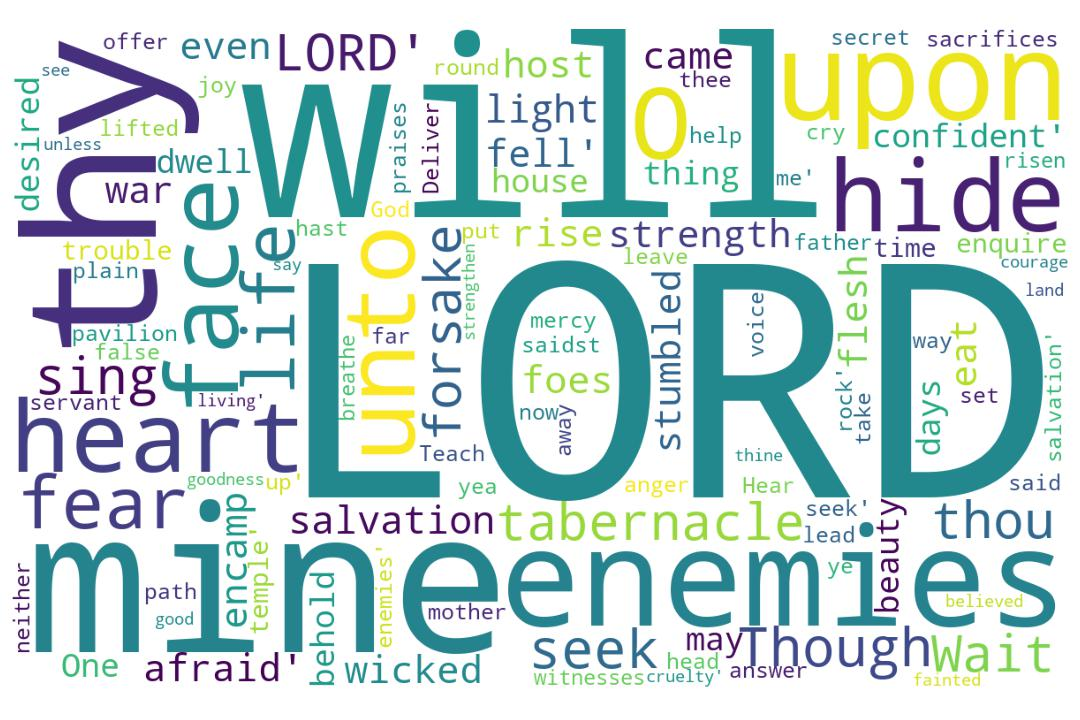
\includegraphics[width=\linewidth]{19OT-Psalms/Psalm27-WordCloud.jpg}
  \caption{Psalm 27 Word Cloud}
  \label{fig:Psalm 27 word Cloud}
\end{figure}

\marginpar{\scriptsize \centering \fcolorbox{bone}{lime}{\textbf{SEEING GOD AT WORK}}\\ (Psalm 27:1-14) \begin{compactenum}[I.][8]
    \item \textbf{Witnessing} the Schemes of the World \index[scripture]{Psalms!Psa 027:3}(Psa 27:3)
    \item \textbf{Witnessing} the Lies of Sinners \index[scripture]{Psalms!Psa 027:12}(Psa 27:12)
    \item \textbf{Wondering} about the Supernatural Miracles to happen 
    \item \textbf{Wanting} the Saviour \index[scripture]{Psalms!Psa 027:8}(Psa 27:8)
    \item \textbf{Waiting} on the LORD's Salvation \index[scripture]{Psalms!Psa 027:14}(Psa 27:14)
    \item \textbf{Watching} the the LORD of Show \index[scripture]{Psalms!Psa 027:6}(Psa 27:6)
\end{compactenum}}

\footnote{\textcolor[cmyk]{0.99998,1,0,0}{\hyperlink{TOC}{Return to end of Table of Contents.}}}\footnote{\href{https://www.audioverse.org/english/audiobibles/books/ENGKJV/O/Ps/1}{\textcolor[cmyk]{0.99998,1,0,0}{Psalms Audio}}}\textcolor[cmyk]{0.99998,1,0,0}{\emph{A Psalm} of David.} \\
\\
\textcolor[cmyk]{0.99998,1,0,0}{The \fcolorbox{bone}{bone}{LORD} \emph{is} my light and my salvation; whom shall \fcolorbox{bone}{bone}{I} fear? the \fcolorbox{bone}{bone}{LORD} \emph{is} the strength of my life; of whom shall \fcolorbox{bone}{bone}{I} be afraid?}
[2] \textcolor[cmyk]{0.99998,1,0,0}{When the wicked, \emph{even} mine enemies and my foes, came upon me to eat up my flesh, they stumbled and fell.}
[3] \textcolor[cmyk]{0.99998,1,0,0}{Though an host should \fcolorbox{bone}{lime}{encamp against} me, my heart shall not fear: though war should rise against me, in this \emph{will} \fcolorbox{bone}{bone}{I} \emph{be} confident.}
[4] \textcolor[cmyk]{0.99998,1,0,0}{One \emph{thing} have \fcolorbox{bone}{bone}{I} desired of the \fcolorbox{bone}{bone}{LORD}, that will \fcolorbox{bone}{bone}{I} seek after; that \fcolorbox{bone}{bone}{I} may dwell in the house of the \fcolorbox{bone}{bone}{LORD} all the days of my life, to behold the beauty of the \fcolorbox{bone}{bone}{LORD}, and to enquire in his temple.}
[5] \textcolor[cmyk]{0.99998,1,0,0}{For in the time of trouble he shall hide me in his pavilion: in the secret of his tabernacle shall he hide me; he shall set me up upon a rock.}
[6] \textcolor[cmyk]{0.99998,1,0,0}{And now shall mine head be lifted up above mine enemies round about me: therefore will \fcolorbox{bone}{bone}{I} offer in his tabernacle \fcolorbox{bone}{lime}{sacrifices of joy}; \fcolorbox{bone}{bone}{I} will sing, yea, \fcolorbox{bone}{bone}{I} will sing praises unto the \fcolorbox{bone}{bone}{LORD}.}
[7] \textcolor[cmyk]{0.99998,1,0,0}{Hear, O \fcolorbox{bone}{bone}{LORD}, \emph{when} \fcolorbox{bone}{bone}{I} cry with my voice: have mercy also upon me, and answer me.}
[8] \textcolor[cmyk]{0.99998,1,0,0}{\emph{When} \emph{thou} \emph{saidst}, Seek ye my face; my heart said unto thee, Thy face, \fcolorbox{bone}{bone}{LORD}, will \fcolorbox{bone}{lime}{\fcolorbox{bone}{bone}{I} seek}.}
[9] \textcolor[cmyk]{0.99998,1,0,0}{Hide not thy face \emph{far} from me; put not thy servant away in anger: thou hast been my help; leave me not, neither forsake me, O God of my salvation.}
[10] \textcolor[cmyk]{0.99998,1,0,0}{When my father and my mother forsake me, then the \fcolorbox{bone}{bone}{LORD} will take me up.}
[11] \textcolor[cmyk]{0.99998,1,0,0}{Teach me thy way, O \fcolorbox{bone}{bone}{LORD}, and lead me in a plain path, because of mine enemies.}
[12] \textcolor[cmyk]{0.99998,1,0,0}{Deliver me not over unto the will of mine enemies: for \fcolorbox{bone}{lime}{false witnesses} are risen up against me, and such as breathe out cruelty.}
[13] \textcolor[cmyk]{0.99998,1,0,0}{\emph{I} \emph{had} \emph{fainted}, unless \fcolorbox{bone}{bone}{I} had believed to see the goodness of the \fcolorbox{bone}{bone}{LORD} in the land of the living.}
[14] \textcolor[cmyk]{0.99998,1,0,0}{Wait on the \fcolorbox{bone}{bone}{LORD}: be of good courage, and he shall strengthen thine heart: \fcolorbox{bone}{lime}{wait}, \fcolorbox{bone}{bone}{I} say, on the \fcolorbox{bone}{bone}{LORD}.}
\section{Psalm 27 Comments}

\subsection{Numeric Nuggets}
The words ``LORD'' and ``I'' are used 13 times in this Psalm. 

\subsection{Introduction}
Consider Steven Cole's exposition of the psalm, entitled \href{https://bible.org/seriespage/psalm-27-overcoming-fear}{``Overcoming Fear''}.

\subsection{Psalm 27:2}
Verse 2 can be taken to speak of literal cannibalism that will occur during the Tribulation period. Consider Psalm 16:4,\footnote{\textbf{Psalm 16:4} - Their sorrows shall be multiplied that hasten after another god: their drink offerings of blood will I not offer, nor take up their names into my lips.} Isaiah 6:13,\footnote{\textbf{Isaiah 6:13} - But yet in it shall be a tenth, and it shall return, and shall be eaten: as a teil tree, and as an oak, whose substance is in them, when they cast their leaves: so the holy seed shall be the substance thereof.} and Revelation 6:11.\footnote{\textbf{Revelation 6:11} - And white robes were given unto every one of them; and it was said unto them, that they should rest yet for a little season, until their fellowservants also and their brethren, that should be killed as they were, should be fulfilled.}\cite{Ruckman1992PsalmsV1} 
%\index[NWIV]{26!Psalms!Psa 27:1}\index[AWIP]{The!Psalms!Psa 27:1}\index[AWIP]{LORD!Psalms!Psa 27:1}\index[AWIP]{LORD!Psalms!Psa 27:1 (2)}\index[AWIP]{\emph{is}!Psalms!Psa 27:1}\index[AWIP]{\emph{is}!Psalms!Psa 27:1 (2)}\index[AWIP]{my!Psalms!Psa 27:1}\index[AWIP]{my!Psalms!Psa 27:1 (2)}\index[AWIP]{my!Psalms!Psa 27:1 (3)}\index[AWIP]{light!Psalms!Psa 27:1}\index[AWIP]{and!Psalms!Psa 27:1}\index[AWIP]{salvation!Psalms!Psa 27:1}\index[AWIP]{whom!Psalms!Psa 27:1}\index[AWIP]{whom!Psalms!Psa 27:1 (2)}\index[AWIP]{shall!Psalms!Psa 27:1}\index[AWIP]{shall!Psalms!Psa 27:1 (2)}\index[AWIP]{I!Psalms!Psa 27:1}\index[AWIP]{I!Psalms!Psa 27:1 (2)}\index[AWIP]{fear?!Psalms!Psa 27:1}\index[AWIP]{the!Psalms!Psa 27:1}\index[AWIP]{the!Psalms!Psa 27:1 (2)}\index[AWIP]{strength!Psalms!Psa 27:1}\index[AWIP]{of!Psalms!Psa 27:1}\index[AWIP]{of!Psalms!Psa 27:1 (2)}\index[AWIP]{life!Psalms!Psa 27:1}\index[AWIP]{be!Psalms!Psa 27:1}\index[AWIP]{afraid?!Psalms!Psa 27:1}\index[AWIP]{\emph{is}!Psalms!Psa 27:1}\index[AWIP]{\emph{is}!Psalms!Psa 27:1 (2)}

\index[NWIV]{21!Psalms!Psa 27:2}\index[AWIP]{When!Psalms!Psa 27:2}\index[AWIP]{the!Psalms!Psa 27:2}\index[AWIP]{wicked!Psalms!Psa 27:2}\index[AWIP]{\emph{even}!Psalms!Psa 27:2}\index[AWIP]{mine!Psalms!Psa 27:2}\index[AWIP]{enemies!Psalms!Psa 27:2}\index[AWIP]{and!Psalms!Psa 27:2}\index[AWIP]{and!Psalms!Psa 27:2 (2)}\index[AWIP]{my!Psalms!Psa 27:2}\index[AWIP]{my!Psalms!Psa 27:2 (2)}\index[AWIP]{foes!Psalms!Psa 27:2}\index[AWIP]{came!Psalms!Psa 27:2}\index[AWIP]{upon!Psalms!Psa 27:2}\index[AWIP]{me!Psalms!Psa 27:2}\index[AWIP]{to!Psalms!Psa 27:2}\index[AWIP]{eat!Psalms!Psa 27:2}\index[AWIP]{up!Psalms!Psa 27:2}\index[AWIP]{flesh!Psalms!Psa 27:2}\index[AWIP]{they!Psalms!Psa 27:2}\index[AWIP]{stumbled!Psalms!Psa 27:2}\index[AWIP]{fell!Psalms!Psa 27:2}\index[AWIP]{\emph{even}!Psalms!Psa 27:2}

\index[NWIV]{24!Psalms!Psa 27:3}\index[AWIP]{Though!Psalms!Psa 27:3}\index[AWIP]{an!Psalms!Psa 27:3}\index[AWIP]{host!Psalms!Psa 27:3}\index[AWIP]{should!Psalms!Psa 27:3}\index[AWIP]{should!Psalms!Psa 27:3 (2)}\index[AWIP]{encamp!Psalms!Psa 27:3}\index[AWIP]{against!Psalms!Psa 27:3}\index[AWIP]{against!Psalms!Psa 27:3 (2)}\index[AWIP]{me!Psalms!Psa 27:3}\index[AWIP]{me!Psalms!Psa 27:3 (2)}\index[AWIP]{my!Psalms!Psa 27:3}\index[AWIP]{heart!Psalms!Psa 27:3}\index[AWIP]{shall!Psalms!Psa 27:3}\index[AWIP]{not!Psalms!Psa 27:3}\index[AWIP]{fear!Psalms!Psa 27:3}\index[AWIP]{though!Psalms!Psa 27:3}\index[AWIP]{war!Psalms!Psa 27:3}\index[AWIP]{rise!Psalms!Psa 27:3}\index[AWIP]{in!Psalms!Psa 27:3}\index[AWIP]{this!Psalms!Psa 27:3}\index[AWIP]{\emph{will}!Psalms!Psa 27:3}\index[AWIP]{I!Psalms!Psa 27:3}\index[AWIP]{\emph{be}!Psalms!Psa 27:3}\index[AWIP]{confident!Psalms!Psa 27:3}\index[AWIP]{\emph{will}!Psalms!Psa 27:3}\index[AWIP]{\emph{be}!Psalms!Psa 27:3}

\index[NWIV]{42!Psalms!Psa 27:4}\index[AWIP]{One!Psalms!Psa 27:4}\index[AWIP]{\emph{thing}!Psalms!Psa 27:4}\index[AWIP]{have!Psalms!Psa 27:4}\index[AWIP]{I!Psalms!Psa 27:4}\index[AWIP]{I!Psalms!Psa 27:4 (2)}\index[AWIP]{I!Psalms!Psa 27:4 (3)}\index[AWIP]{desired!Psalms!Psa 27:4}\index[AWIP]{of!Psalms!Psa 27:4}\index[AWIP]{of!Psalms!Psa 27:4 (2)}\index[AWIP]{of!Psalms!Psa 27:4 (3)}\index[AWIP]{of!Psalms!Psa 27:4 (4)}\index[AWIP]{the!Psalms!Psa 27:4}\index[AWIP]{the!Psalms!Psa 27:4 (2)}\index[AWIP]{the!Psalms!Psa 27:4 (3)}\index[AWIP]{the!Psalms!Psa 27:4 (4)}\index[AWIP]{the!Psalms!Psa 27:4 (5)}\index[AWIP]{the!Psalms!Psa 27:4 (6)}\index[AWIP]{LORD!Psalms!Psa 27:4}\index[AWIP]{LORD!Psalms!Psa 27:4 (2)}\index[AWIP]{LORD!Psalms!Psa 27:4 (3)}\index[AWIP]{that!Psalms!Psa 27:4}\index[AWIP]{that!Psalms!Psa 27:4 (2)}\index[AWIP]{will!Psalms!Psa 27:4}\index[AWIP]{seek!Psalms!Psa 27:4}\index[AWIP]{after!Psalms!Psa 27:4}\index[AWIP]{may!Psalms!Psa 27:4}\index[AWIP]{dwell!Psalms!Psa 27:4}\index[AWIP]{in!Psalms!Psa 27:4}\index[AWIP]{in!Psalms!Psa 27:4 (2)}\index[AWIP]{house!Psalms!Psa 27:4}\index[AWIP]{all!Psalms!Psa 27:4}\index[AWIP]{days!Psalms!Psa 27:4}\index[AWIP]{my!Psalms!Psa 27:4}\index[AWIP]{life!Psalms!Psa 27:4}\index[AWIP]{to!Psalms!Psa 27:4}\index[AWIP]{to!Psalms!Psa 27:4 (2)}\index[AWIP]{behold!Psalms!Psa 27:4}\index[AWIP]{beauty!Psalms!Psa 27:4}\index[AWIP]{and!Psalms!Psa 27:4}\index[AWIP]{enquire!Psalms!Psa 27:4}\index[AWIP]{his!Psalms!Psa 27:4}\index[AWIP]{temple!Psalms!Psa 27:4}\index[AWIP]{\emph{thing}!Psalms!Psa 27:4}

\index[NWIV]{31!Psalms!Psa 27:5}\index[AWIP]{For!Psalms!Psa 27:5}\index[AWIP]{in!Psalms!Psa 27:5}\index[AWIP]{in!Psalms!Psa 27:5 (2)}\index[AWIP]{in!Psalms!Psa 27:5 (3)}\index[AWIP]{the!Psalms!Psa 27:5}\index[AWIP]{the!Psalms!Psa 27:5 (2)}\index[AWIP]{time!Psalms!Psa 27:5}\index[AWIP]{of!Psalms!Psa 27:5}\index[AWIP]{of!Psalms!Psa 27:5 (2)}\index[AWIP]{trouble!Psalms!Psa 27:5}\index[AWIP]{he!Psalms!Psa 27:5}\index[AWIP]{he!Psalms!Psa 27:5 (2)}\index[AWIP]{he!Psalms!Psa 27:5 (3)}\index[AWIP]{shall!Psalms!Psa 27:5}\index[AWIP]{shall!Psalms!Psa 27:5 (2)}\index[AWIP]{shall!Psalms!Psa 27:5 (3)}\index[AWIP]{hide!Psalms!Psa 27:5}\index[AWIP]{hide!Psalms!Psa 27:5 (2)}\index[AWIP]{me!Psalms!Psa 27:5}\index[AWIP]{me!Psalms!Psa 27:5 (2)}\index[AWIP]{me!Psalms!Psa 27:5 (3)}\index[AWIP]{his!Psalms!Psa 27:5}\index[AWIP]{his!Psalms!Psa 27:5 (2)}\index[AWIP]{pavilion!Psalms!Psa 27:5}\index[AWIP]{secret!Psalms!Psa 27:5}\index[AWIP]{tabernacle!Psalms!Psa 27:5}\index[AWIP]{set!Psalms!Psa 27:5}\index[AWIP]{up!Psalms!Psa 27:5}\index[AWIP]{upon!Psalms!Psa 27:5}\index[AWIP]{a!Psalms!Psa 27:5}\index[AWIP]{rock!Psalms!Psa 27:5}

\index[NWIV]{35!Psalms!Psa 27:6}\index[AWIP]{And!Psalms!Psa 27:6}\index[AWIP]{now!Psalms!Psa 27:6}\index[AWIP]{shall!Psalms!Psa 27:6}\index[AWIP]{mine!Psalms!Psa 27:6}\index[AWIP]{mine!Psalms!Psa 27:6 (2)}\index[AWIP]{head!Psalms!Psa 27:6}\index[AWIP]{be!Psalms!Psa 27:6}\index[AWIP]{lifted!Psalms!Psa 27:6}\index[AWIP]{up!Psalms!Psa 27:6}\index[AWIP]{above!Psalms!Psa 27:6}\index[AWIP]{enemies!Psalms!Psa 27:6}\index[AWIP]{round!Psalms!Psa 27:6}\index[AWIP]{about!Psalms!Psa 27:6}\index[AWIP]{me!Psalms!Psa 27:6}\index[AWIP]{therefore!Psalms!Psa 27:6}\index[AWIP]{will!Psalms!Psa 27:6}\index[AWIP]{will!Psalms!Psa 27:6 (2)}\index[AWIP]{will!Psalms!Psa 27:6 (3)}\index[AWIP]{I!Psalms!Psa 27:6}\index[AWIP]{I!Psalms!Psa 27:6 (2)}\index[AWIP]{I!Psalms!Psa 27:6 (3)}\index[AWIP]{offer!Psalms!Psa 27:6}\index[AWIP]{in!Psalms!Psa 27:6}\index[AWIP]{his!Psalms!Psa 27:6}\index[AWIP]{tabernacle!Psalms!Psa 27:6}\index[AWIP]{sacrifices!Psalms!Psa 27:6}\index[AWIP]{of!Psalms!Psa 27:6}\index[AWIP]{joy!Psalms!Psa 27:6}\index[AWIP]{sing!Psalms!Psa 27:6}\index[AWIP]{sing!Psalms!Psa 27:6 (2)}\index[AWIP]{yea!Psalms!Psa 27:6}\index[AWIP]{praises!Psalms!Psa 27:6}\index[AWIP]{unto!Psalms!Psa 27:6}\index[AWIP]{the!Psalms!Psa 27:6}\index[AWIP]{LORD!Psalms!Psa 27:6}

\index[NWIV]{17!Psalms!Psa 27:7}\index[AWIP]{Hear!Psalms!Psa 27:7}\index[AWIP]{O!Psalms!Psa 27:7}\index[AWIP]{LORD!Psalms!Psa 27:7}\index[AWIP]{\emph{when}!Psalms!Psa 27:7}\index[AWIP]{I!Psalms!Psa 27:7}\index[AWIP]{cry!Psalms!Psa 27:7}\index[AWIP]{with!Psalms!Psa 27:7}\index[AWIP]{my!Psalms!Psa 27:7}\index[AWIP]{voice!Psalms!Psa 27:7}\index[AWIP]{have!Psalms!Psa 27:7}\index[AWIP]{mercy!Psalms!Psa 27:7}\index[AWIP]{also!Psalms!Psa 27:7}\index[AWIP]{upon!Psalms!Psa 27:7}\index[AWIP]{me!Psalms!Psa 27:7}\index[AWIP]{me!Psalms!Psa 27:7 (2)}\index[AWIP]{and!Psalms!Psa 27:7}\index[AWIP]{answer!Psalms!Psa 27:7}\index[AWIP]{\emph{when}!Psalms!Psa 27:7}

\index[NWIV]{18!Psalms!Psa 27:8}\index[AWIP]{\emph{When}!Psalms!Psa 27:8}\index[AWIP]{\emph{thou}!Psalms!Psa 27:8}\index[AWIP]{\emph{saidst}!Psalms!Psa 27:8}\index[AWIP]{Seek!Psalms!Psa 27:8}\index[AWIP]{ye!Psalms!Psa 27:8}\index[AWIP]{my!Psalms!Psa 27:8}\index[AWIP]{my!Psalms!Psa 27:8 (2)}\index[AWIP]{face!Psalms!Psa 27:8}\index[AWIP]{face!Psalms!Psa 27:8 (2)}\index[AWIP]{heart!Psalms!Psa 27:8}\index[AWIP]{said!Psalms!Psa 27:8}\index[AWIP]{unto!Psalms!Psa 27:8}\index[AWIP]{thee!Psalms!Psa 27:8}\index[AWIP]{Thy!Psalms!Psa 27:8}\index[AWIP]{LORD!Psalms!Psa 27:8}\index[AWIP]{will!Psalms!Psa 27:8}\index[AWIP]{I!Psalms!Psa 27:8}\index[AWIP]{seek!Psalms!Psa 27:8}\index[AWIP]{\emph{When}!Psalms!Psa 27:8}\index[AWIP]{\emph{thou}!Psalms!Psa 27:8}\index[AWIP]{\emph{saidst}!Psalms!Psa 27:8}

\index[NWIV]{30!Psalms!Psa 27:9}\index[AWIP]{Hide!Psalms!Psa 27:9}\index[AWIP]{not!Psalms!Psa 27:9}\index[AWIP]{not!Psalms!Psa 27:9 (2)}\index[AWIP]{not!Psalms!Psa 27:9 (3)}\index[AWIP]{thy!Psalms!Psa 27:9}\index[AWIP]{thy!Psalms!Psa 27:9 (2)}\index[AWIP]{face!Psalms!Psa 27:9}\index[AWIP]{\emph{far}!Psalms!Psa 27:9}\index[AWIP]{from!Psalms!Psa 27:9}\index[AWIP]{me!Psalms!Psa 27:9}\index[AWIP]{me!Psalms!Psa 27:9 (2)}\index[AWIP]{me!Psalms!Psa 27:9 (3)}\index[AWIP]{put!Psalms!Psa 27:9}\index[AWIP]{servant!Psalms!Psa 27:9}\index[AWIP]{away!Psalms!Psa 27:9}\index[AWIP]{in!Psalms!Psa 27:9}\index[AWIP]{anger!Psalms!Psa 27:9}\index[AWIP]{thou!Psalms!Psa 27:9}\index[AWIP]{hast!Psalms!Psa 27:9}\index[AWIP]{been!Psalms!Psa 27:9}\index[AWIP]{my!Psalms!Psa 27:9}\index[AWIP]{my!Psalms!Psa 27:9 (2)}\index[AWIP]{help!Psalms!Psa 27:9}\index[AWIP]{leave!Psalms!Psa 27:9}\index[AWIP]{neither!Psalms!Psa 27:9}\index[AWIP]{forsake!Psalms!Psa 27:9}\index[AWIP]{O!Psalms!Psa 27:9}\index[AWIP]{God!Psalms!Psa 27:9}\index[AWIP]{of!Psalms!Psa 27:9}\index[AWIP]{salvation!Psalms!Psa 27:9}\index[AWIP]{\emph{far}!Psalms!Psa 27:9}

\index[NWIV]{15!Psalms!Psa 27:10}\index[AWIP]{When!Psalms!Psa 27:10}\index[AWIP]{my!Psalms!Psa 27:10}\index[AWIP]{my!Psalms!Psa 27:10 (2)}\index[AWIP]{father!Psalms!Psa 27:10}\index[AWIP]{and!Psalms!Psa 27:10}\index[AWIP]{mother!Psalms!Psa 27:10}\index[AWIP]{forsake!Psalms!Psa 27:10}\index[AWIP]{me!Psalms!Psa 27:10}\index[AWIP]{me!Psalms!Psa 27:10 (2)}\index[AWIP]{then!Psalms!Psa 27:10}\index[AWIP]{the!Psalms!Psa 27:10}\index[AWIP]{LORD!Psalms!Psa 27:10}\index[AWIP]{will!Psalms!Psa 27:10}\index[AWIP]{take!Psalms!Psa 27:10}\index[AWIP]{up!Psalms!Psa 27:10}

\index[NWIV]{17!Psalms!Psa 27:11}\index[AWIP]{Teach!Psalms!Psa 27:11}\index[AWIP]{me!Psalms!Psa 27:11}\index[AWIP]{me!Psalms!Psa 27:11 (2)}\index[AWIP]{thy!Psalms!Psa 27:11}\index[AWIP]{way!Psalms!Psa 27:11}\index[AWIP]{O!Psalms!Psa 27:11}\index[AWIP]{LORD!Psalms!Psa 27:11}\index[AWIP]{and!Psalms!Psa 27:11}\index[AWIP]{lead!Psalms!Psa 27:11}\index[AWIP]{in!Psalms!Psa 27:11}\index[AWIP]{a!Psalms!Psa 27:11}\index[AWIP]{plain!Psalms!Psa 27:11}\index[AWIP]{path!Psalms!Psa 27:11}\index[AWIP]{because!Psalms!Psa 27:11}\index[AWIP]{of!Psalms!Psa 27:11}\index[AWIP]{mine!Psalms!Psa 27:11}\index[AWIP]{enemies!Psalms!Psa 27:11}

\index[NWIV]{24!Psalms!Psa 27:12}\index[AWIP]{Deliver!Psalms!Psa 27:12}\index[AWIP]{me!Psalms!Psa 27:12}\index[AWIP]{me!Psalms!Psa 27:12 (2)}\index[AWIP]{not!Psalms!Psa 27:12}\index[AWIP]{over!Psalms!Psa 27:12}\index[AWIP]{unto!Psalms!Psa 27:12}\index[AWIP]{the!Psalms!Psa 27:12}\index[AWIP]{will!Psalms!Psa 27:12}\index[AWIP]{of!Psalms!Psa 27:12}\index[AWIP]{mine!Psalms!Psa 27:12}\index[AWIP]{enemies!Psalms!Psa 27:12}\index[AWIP]{for!Psalms!Psa 27:12}\index[AWIP]{false!Psalms!Psa 27:12}\index[AWIP]{witnesses!Psalms!Psa 27:12}\index[AWIP]{are!Psalms!Psa 27:12}\index[AWIP]{risen!Psalms!Psa 27:12}\index[AWIP]{up!Psalms!Psa 27:12}\index[AWIP]{against!Psalms!Psa 27:12}\index[AWIP]{and!Psalms!Psa 27:12}\index[AWIP]{such!Psalms!Psa 27:12}\index[AWIP]{as!Psalms!Psa 27:12}\index[AWIP]{breathe!Psalms!Psa 27:12}\index[AWIP]{out!Psalms!Psa 27:12}\index[AWIP]{cruelty!Psalms!Psa 27:12}

\index[NWIV]{20!Psalms!Psa 27:13}\index[AWIP]{\emph{I}!Psalms!Psa 27:13}\index[AWIP]{\emph{had}!Psalms!Psa 27:13}\index[AWIP]{\emph{fainted}!Psalms!Psa 27:13}\index[AWIP]{unless!Psalms!Psa 27:13}\index[AWIP]{I!Psalms!Psa 27:13}\index[AWIP]{had!Psalms!Psa 27:13}\index[AWIP]{believed!Psalms!Psa 27:13}\index[AWIP]{to!Psalms!Psa 27:13}\index[AWIP]{see!Psalms!Psa 27:13}\index[AWIP]{the!Psalms!Psa 27:13}\index[AWIP]{the!Psalms!Psa 27:13 (2)}\index[AWIP]{the!Psalms!Psa 27:13 (3)}\index[AWIP]{the!Psalms!Psa 27:13 (4)}\index[AWIP]{goodness!Psalms!Psa 27:13}\index[AWIP]{of!Psalms!Psa 27:13}\index[AWIP]{of!Psalms!Psa 27:13 (2)}\index[AWIP]{LORD!Psalms!Psa 27:13}\index[AWIP]{in!Psalms!Psa 27:13}\index[AWIP]{land!Psalms!Psa 27:13}\index[AWIP]{living!Psalms!Psa 27:13}\index[AWIP]{\emph{I}!Psalms!Psa 27:13}\index[AWIP]{\emph{had}!Psalms!Psa 27:13}\index[AWIP]{\emph{fainted}!Psalms!Psa 27:13}

\index[NWIV]{20!Psalms!Psa 27:14}\index[AWIP]{Wait!Psalms!Psa 27:14}\index[AWIP]{on!Psalms!Psa 27:14}\index[AWIP]{on!Psalms!Psa 27:14 (2)}\index[AWIP]{the!Psalms!Psa 27:14}\index[AWIP]{the!Psalms!Psa 27:14 (2)}\index[AWIP]{LORD!Psalms!Psa 27:14}\index[AWIP]{LORD!Psalms!Psa 27:14 (2)}\index[AWIP]{be!Psalms!Psa 27:14}\index[AWIP]{of!Psalms!Psa 27:14}\index[AWIP]{good!Psalms!Psa 27:14}\index[AWIP]{courage!Psalms!Psa 27:14}\index[AWIP]{and!Psalms!Psa 27:14}\index[AWIP]{he!Psalms!Psa 27:14}\index[AWIP]{shall!Psalms!Psa 27:14}\index[AWIP]{strengthen!Psalms!Psa 27:14}\index[AWIP]{thine!Psalms!Psa 27:14}\index[AWIP]{heart!Psalms!Psa 27:14}\index[AWIP]{wait!Psalms!Psa 27:14}\index[AWIP]{I!Psalms!Psa 27:14}\index[AWIP]{say!Psalms!Psa 27:14}


\section{Psalm 27 Outlines}

\subsection{My Outlines}

\subsubsection{Seeing God at Work}

\index[speaker]{Keith Anthony!Psalm 027 (Seeing God at Work)}
\index[series]{Psalms (Keith Anthony)!Psalm 027 (Seeing God at Work)}
\index[date]{2016/07/01!Psalm 027 (Seeing God at Work) (Keith Anthony)}
\begin{compactenum}[I.]
    \item \textbf{Witnessing} the Schemes of the World \index[scripture]{Psalms!Psa 027:3}(Psa 27:3)
    \item \textbf{Witnessing} the Lies of Sinners \index[scripture]{Psalms!Psa 027:12}(Psa 27:12)
    \item \textbf{Wondering} about the Supernatural Miracles to happen 
    \item \textbf{Wanting} the Saviour \index[scripture]{Psalms!Psa 027:8}(Psa 27:8)
    \item \textbf{Waiting} on the Lord's Salvation \index[scripture]{Psalms!Psa 027:14}(Psa 27:14)
    \item \textbf{Watching} the the Lord of Show \index[scripture]{Psalms!Psa 027:6}(Psa 27:6)
\end{compactenum}

\subsection{Outlines from Others}


%\section{Psalm 27 Statistics}

%%%%%%%%%%%%%%%%%%%%%%%%%%%
%%%%% Word Statistics
%%%%%%%%%%%%%%%%%%%%%%%%%%


\normalsize



\subsection{Chapter Word Statistics}


%%%%%%%%%%
%%%%%%%%%%
 
\begin{center}
\begin{longtable}{l|c|c|c|c}
\caption[Stats for Psalm 27]{Stats for Psalm 27} \label{table:Stats for Psalm 27} \\ 
\hline \multicolumn{1}{|c|}{\textbf{Verse(s)}} & \multicolumn{1}{|c|}{\textbf{Count}} & \multicolumn{1}{|c|}{\textbf{Unique}} & \multicolumn{1}{|c|}{\textbf{Italics}} & \multicolumn{1}{|c|}{\textbf{Uniq Italic}}  \\ \hline 
\endfirsthead
 
\multicolumn{5}{c}
{{\bfseries \tablename\ \thetable{} -- continued from previous page}} \\  
\hline \multicolumn{1}{|c|}{\textbf{Verse(s)}} & \multicolumn{1}{|c|}{\textbf{Count}} & \multicolumn{1}{|c|}{\textbf{Unique}} & \multicolumn{1}{|c|}{\textbf{Italics}} & \multicolumn{1}{|c|}{\textbf{Uniq Italic}}  \\ \hline 
\endhead
 
\hline \multicolumn{5}{|r|}{{Continued if needed}} \\ \hline
\endfoot 
1 & 26 & 17 & 2 & 1\\ \hline
2 & 21 & 19 & 1 & 1\\ \hline
3 & 24 & 21 & 2 & 2\\ \hline
4 & 42 & 27 & 1 & 1\\ \hline
5 & 31 & 19 & 0 & 0\\ \hline
6 & 35 & 29 & 0 & 0\\ \hline
7 & 17 & 16 & 1 & 1\\ \hline
8 & 18 & 16 & 3 & 3\\ \hline
9 & 30 & 24 & 1 & 1\\ \hline
10 & 15 & 13 & 0 & 0\\ \hline
11 & 17 & 16 & 0 & 0\\ \hline
12 & 24 & 23 & 0 & 0\\ \hline
13 & 20 & 16 & 3 & 3\\ \hline
14 & 20 & 17 & 0 & 0\\ \hline
\hline \hline
Total & 340 & 167 & 14 & 13



\end{longtable}
\end{center}

%%%%%%%%%%
%%%%%%%%%%
 
\subsection{Words by Frequency}

\begin{center}
\begin{longtable}{l|r}
\caption[Word Frequencies in Psalm 27]{Word Frequencies in Psalm 27} \label{table:WordsIn-Psalm-27} \\ 
\hline \multicolumn{1}{|c|}{\textbf{Word}} & \multicolumn{1}{c|}{\textbf{Frequency}} \\ \hline 
\endfirsthead
 
\multicolumn{2}{c}
{{\bfseries \tablename\ \thetable{} -- continued from previous page}} \\ 
\hline \multicolumn{1}{|c|}{\textbf{Word}} & \multicolumn{1}{c|}{\textbf{Frequency}} \\ \hline 
\endhead
 
\hline \multicolumn{2}{|r|}{{Continued if needed}} \\ \hline
\endfoot
 
\hline \hline
\endlastfoot
the & 20 \\ \hline
me & 18 \\ \hline
of & 15 \\ \hline
my & 14 \\ \hline
LORD & 13 \\ \hline
I & 13 \\ \hline
in & 10 \\ \hline
and & 9 \\ \hline
shall & 8 \\ \hline
will & 7 \\ \hline
mine & 5 \\ \hline
up & 5 \\ \hline
not & 5 \\ \hline
enemies & 4 \\ \hline
to & 4 \\ \hline
his & 4 \\ \hline
he & 4 \\ \hline
be & 3 \\ \hline
upon & 3 \\ \hline
against & 3 \\ \hline
heart & 3 \\ \hline
unto & 3 \\ \hline
O & 3 \\ \hline
face & 3 \\ \hline
thy & 3 \\ \hline
\emph{is} & 2 \\ \hline
salvation & 2 \\ \hline
whom & 2 \\ \hline
fear & 2 \\ \hline
life & 2 \\ \hline
When & 2 \\ \hline
should & 2 \\ \hline
have & 2 \\ \hline
that & 2 \\ \hline
seek & 2 \\ \hline
hide & 2 \\ \hline
tabernacle & 2 \\ \hline
a & 2 \\ \hline
sing & 2 \\ \hline
forsake & 2 \\ \hline
on & 2 \\ \hline
The & 1 \\ \hline
light & 1 \\ \hline
strength & 1 \\ \hline
afraid & 1 \\ \hline
wicked & 1 \\ \hline
\emph{even} & 1 \\ \hline
foes & 1 \\ \hline
came & 1 \\ \hline
eat & 1 \\ \hline
flesh & 1 \\ \hline
they & 1 \\ \hline
stumbled & 1 \\ \hline
fell & 1 \\ \hline
Though & 1 \\ \hline
an & 1 \\ \hline
host & 1 \\ \hline
encamp & 1 \\ \hline
though & 1 \\ \hline
war & 1 \\ \hline
rise & 1 \\ \hline
this & 1 \\ \hline
\emph{will} & 1 \\ \hline
\emph{be} & 1 \\ \hline
confident & 1 \\ \hline
One & 1 \\ \hline
\emph{thing} & 1 \\ \hline
desired & 1 \\ \hline
after & 1 \\ \hline
may & 1 \\ \hline
dwell & 1 \\ \hline
house & 1 \\ \hline
all & 1 \\ \hline
days & 1 \\ \hline
behold & 1 \\ \hline
beauty & 1 \\ \hline
enquire & 1 \\ \hline
temple & 1 \\ \hline
For & 1 \\ \hline
time & 1 \\ \hline
trouble & 1 \\ \hline
pavilion & 1 \\ \hline
secret & 1 \\ \hline
set & 1 \\ \hline
rock & 1 \\ \hline
And & 1 \\ \hline
now & 1 \\ \hline
head & 1 \\ \hline
lifted & 1 \\ \hline
above & 1 \\ \hline
round & 1 \\ \hline
about & 1 \\ \hline
therefore & 1 \\ \hline
offer & 1 \\ \hline
sacrifices & 1 \\ \hline
joy & 1 \\ \hline
yea & 1 \\ \hline
praises & 1 \\ \hline
Hear & 1 \\ \hline
\emph{when} & 1 \\ \hline
cry & 1 \\ \hline
with & 1 \\ \hline
voice & 1 \\ \hline
mercy & 1 \\ \hline
also & 1 \\ \hline
answer & 1 \\ \hline
\emph{When} & 1 \\ \hline
\emph{thou} & 1 \\ \hline
\emph{saidst} & 1 \\ \hline
Seek & 1 \\ \hline
ye & 1 \\ \hline
said & 1 \\ \hline
thee & 1 \\ \hline
Thy & 1 \\ \hline
Hide & 1 \\ \hline
\emph{far} & 1 \\ \hline
from & 1 \\ \hline
put & 1 \\ \hline
servant & 1 \\ \hline
away & 1 \\ \hline
anger & 1 \\ \hline
thou & 1 \\ \hline
hast & 1 \\ \hline
been & 1 \\ \hline
help & 1 \\ \hline
leave & 1 \\ \hline
neither & 1 \\ \hline
God & 1 \\ \hline
father & 1 \\ \hline
mother & 1 \\ \hline
then & 1 \\ \hline
take & 1 \\ \hline
Teach & 1 \\ \hline
way & 1 \\ \hline
lead & 1 \\ \hline
plain & 1 \\ \hline
path & 1 \\ \hline
because & 1 \\ \hline
Deliver & 1 \\ \hline
over & 1 \\ \hline
for & 1 \\ \hline
false & 1 \\ \hline
witnesses & 1 \\ \hline
are & 1 \\ \hline
risen & 1 \\ \hline
such & 1 \\ \hline
as & 1 \\ \hline
breathe & 1 \\ \hline
out & 1 \\ \hline
cruelty & 1 \\ \hline
\emph{I} & 1 \\ \hline
\emph{had} & 1 \\ \hline
\emph{fainted} & 1 \\ \hline
unless & 1 \\ \hline
had & 1 \\ \hline
believed & 1 \\ \hline
see & 1 \\ \hline
goodness & 1 \\ \hline
land & 1 \\ \hline
living & 1 \\ \hline
Wait & 1 \\ \hline
good & 1 \\ \hline
courage & 1 \\ \hline
strengthen & 1 \\ \hline
thine & 1 \\ \hline
wait & 1 \\ \hline
say & 1 \\ \hline
\end{longtable}
\end{center}



\normalsize



\subsection{Words Alphabetically}

\begin{center}
\begin{longtable}{l|r}
\caption[Word Alphabetically in Psalm 27]{Word Alphabetically in Psalm 27} \label{table:WordsIn-Psalm-27} \\ 
\hline \multicolumn{1}{|c|}{\textbf{Word}} & \multicolumn{1}{c|}{\textbf{Frequency}} \\ \hline 
\endfirsthead
 
\multicolumn{2}{c}
{{\bfseries \tablename\ \thetable{} -- continued from previous page}} \\ 
\hline \multicolumn{1}{|c|}{\textbf{Word}} & \multicolumn{1}{c|}{\textbf{Frequency}} \\ \hline 
\endhead
 
\hline \multicolumn{2}{|r|}{{Continued if needed}} \\ \hline
\endfoot
 
\hline \hline
\endlastfoot
And & 1 \\ \hline
Deliver & 1 \\ \hline
For & 1 \\ \hline
God & 1 \\ \hline
Hear & 1 \\ \hline
Hide & 1 \\ \hline
I & 13 \\ \hline
LORD & 13 \\ \hline
O & 3 \\ \hline
One & 1 \\ \hline
Seek & 1 \\ \hline
Teach & 1 \\ \hline
The & 1 \\ \hline
Though & 1 \\ \hline
Thy & 1 \\ \hline
Wait & 1 \\ \hline
When & 2 \\ \hline
\emph{I} & 1 \\ \hline
\emph{When} & 1 \\ \hline
\emph{be} & 1 \\ \hline
\emph{even} & 1 \\ \hline
\emph{fainted} & 1 \\ \hline
\emph{far} & 1 \\ \hline
\emph{had} & 1 \\ \hline
\emph{is} & 2 \\ \hline
\emph{saidst} & 1 \\ \hline
\emph{thing} & 1 \\ \hline
\emph{thou} & 1 \\ \hline
\emph{when} & 1 \\ \hline
\emph{will} & 1 \\ \hline
a & 2 \\ \hline
about & 1 \\ \hline
above & 1 \\ \hline
afraid & 1 \\ \hline
after & 1 \\ \hline
against & 3 \\ \hline
all & 1 \\ \hline
also & 1 \\ \hline
an & 1 \\ \hline
and & 9 \\ \hline
anger & 1 \\ \hline
answer & 1 \\ \hline
are & 1 \\ \hline
as & 1 \\ \hline
away & 1 \\ \hline
be & 3 \\ \hline
beauty & 1 \\ \hline
because & 1 \\ \hline
been & 1 \\ \hline
behold & 1 \\ \hline
believed & 1 \\ \hline
breathe & 1 \\ \hline
came & 1 \\ \hline
confident & 1 \\ \hline
courage & 1 \\ \hline
cruelty & 1 \\ \hline
cry & 1 \\ \hline
days & 1 \\ \hline
desired & 1 \\ \hline
dwell & 1 \\ \hline
eat & 1 \\ \hline
encamp & 1 \\ \hline
enemies & 4 \\ \hline
enquire & 1 \\ \hline
face & 3 \\ \hline
false & 1 \\ \hline
father & 1 \\ \hline
fear & 2 \\ \hline
fell & 1 \\ \hline
flesh & 1 \\ \hline
foes & 1 \\ \hline
for & 1 \\ \hline
forsake & 2 \\ \hline
from & 1 \\ \hline
good & 1 \\ \hline
goodness & 1 \\ \hline
had & 1 \\ \hline
hast & 1 \\ \hline
have & 2 \\ \hline
he & 4 \\ \hline
head & 1 \\ \hline
heart & 3 \\ \hline
help & 1 \\ \hline
hide & 2 \\ \hline
his & 4 \\ \hline
host & 1 \\ \hline
house & 1 \\ \hline
in & 10 \\ \hline
joy & 1 \\ \hline
land & 1 \\ \hline
lead & 1 \\ \hline
leave & 1 \\ \hline
life & 2 \\ \hline
lifted & 1 \\ \hline
light & 1 \\ \hline
living & 1 \\ \hline
may & 1 \\ \hline
me & 18 \\ \hline
mercy & 1 \\ \hline
mine & 5 \\ \hline
mother & 1 \\ \hline
my & 14 \\ \hline
neither & 1 \\ \hline
not & 5 \\ \hline
now & 1 \\ \hline
of & 15 \\ \hline
offer & 1 \\ \hline
on & 2 \\ \hline
out & 1 \\ \hline
over & 1 \\ \hline
path & 1 \\ \hline
pavilion & 1 \\ \hline
plain & 1 \\ \hline
praises & 1 \\ \hline
put & 1 \\ \hline
rise & 1 \\ \hline
risen & 1 \\ \hline
rock & 1 \\ \hline
round & 1 \\ \hline
sacrifices & 1 \\ \hline
said & 1 \\ \hline
salvation & 2 \\ \hline
say & 1 \\ \hline
secret & 1 \\ \hline
see & 1 \\ \hline
seek & 2 \\ \hline
servant & 1 \\ \hline
set & 1 \\ \hline
shall & 8 \\ \hline
should & 2 \\ \hline
sing & 2 \\ \hline
strength & 1 \\ \hline
strengthen & 1 \\ \hline
stumbled & 1 \\ \hline
such & 1 \\ \hline
tabernacle & 2 \\ \hline
take & 1 \\ \hline
temple & 1 \\ \hline
that & 2 \\ \hline
the & 20 \\ \hline
thee & 1 \\ \hline
then & 1 \\ \hline
therefore & 1 \\ \hline
they & 1 \\ \hline
thine & 1 \\ \hline
this & 1 \\ \hline
thou & 1 \\ \hline
though & 1 \\ \hline
thy & 3 \\ \hline
time & 1 \\ \hline
to & 4 \\ \hline
trouble & 1 \\ \hline
unless & 1 \\ \hline
unto & 3 \\ \hline
up & 5 \\ \hline
upon & 3 \\ \hline
voice & 1 \\ \hline
wait & 1 \\ \hline
war & 1 \\ \hline
way & 1 \\ \hline
whom & 2 \\ \hline
wicked & 1 \\ \hline
will & 7 \\ \hline
with & 1 \\ \hline
witnesses & 1 \\ \hline
ye & 1 \\ \hline
yea & 1 \\ \hline
\end{longtable}
\end{center}



\normalsize



\subsection{Word Lengths in Chapter}
\normalsize
\begin{longtable}{l|p{3.75in}}
\caption[Words by Length in Psalm 27]{Words by Length in Psalm 27} \label{table:WordsIn-Psalm-27} \\ 
\hline \multicolumn{1}{|c|}{\textbf{Length}} & \multicolumn{1}{c|}{\textbf{Words}} \\ \hline 
\endfirsthead
 
\multicolumn{2}{c}
{{\bfseries \tablename\ \thetable{} -- continued from previous page}} \\ 
\hline \multicolumn{1}{|c|}{\textbf{Length}} & \multicolumn{1}{c|}{\textbf{Words}} \\ \hline 
\endhead
 
\hline \multicolumn{2}{|r|}{{Continued if needed}} \\ \hline
\endfoot
 
\hline \hline
\endlastfoot
1 & I, a, O, \emph{I} \\ \hline
2 & \emph{is}, my, of, be, me, to, up, an, in, \emph{be}, he, ye, as, on \\ \hline
3 & The, and, the, eat, not, war, One, may, all, his, For, set, And, now, joy, yea, cry, Thy, thy, \emph{far}, put, God, way, for, are, out, \emph{had}, had, see, say \\ \hline
4 & LORD, whom, fear, life, When, \emph{even}, mine, foes, came, upon, they, fell, host, rise, this, \emph{will}, have, that, will, seek, days, time, hide, rock, head, sing, unto, Hear, \emph{when}, with, also, \emph{When}, \emph{thou}, Seek, face, said, thee, Hide, from, away, thou, hast, been, help, then, take, lead, path, over, such, land, Wait, good, wait \\ \hline
5 & light, shall, flesh, heart, \emph{thing}, after, dwell, house, above, round, about, offer, voice, mercy, anger, leave, Teach, plain, false, risen, thine \\ \hline
6 & afraid, wicked, Though, should, encamp, though, behold, beauty, temple, secret, lifted, answer, \emph{saidst}, father, mother, unless, living \\ \hline
7 & enemies, against, desired, enquire, trouble, praises, servant, neither, forsake, because, Deliver, breathe, cruelty, \emph{fainted}, courage \\ \hline
8 & strength, stumbled, pavilion, believed, goodness \\ \hline
9 & salvation, confident, therefore, witnesses \\ \hline
10 & tabernacle, sacrifices, strengthen \\ \hline
\end{longtable}






%%%%%%%%%%
%%%%%%%%%%
 



%%%%%%%%%%
%%%%%%%%%%
\subsection{Verses with 18 Words in Chapter}
\normalsize
\begin{longtable}{l|p{3.75in}}
\caption[Verses with 18 Words  in Psalm 27]{Verses with 18 Words  in Psalm 27} \label{table:Verses with 18 Words in-Psalm-27} \\ 
\hline \multicolumn{1}{|c|}{\textbf{Reference}} & \multicolumn{1}{c|}{\textbf{Verse}} \\ \hline 
\endfirsthead
 
\multicolumn{2}{c}
{{\bfseries \tablename\ \thetable{} -- continued from previous page}} \\ 
\hline \multicolumn{1}{|c|}{\textbf{Reference}} & \multicolumn{1}{c|}{\textbf{Verse}} \\ \hline 
\endhead
 
\hline \multicolumn{2}{|r|}{{Continued if needed}} \\ \hline
\endfoot
 
\hline \hline
\endlastfoot
Psalms 027:8 & \emph{When} \emph{thou} \emph{saidst}, Seek ye my face; my heart said unto thee, Thy face, LORD, will I seek. \\ \hline
\end{longtable}






%%%%%%%%%%
%%%%%%%%%%
\subsection{Psalm 27 Repeated Phrases}


%%%%%%%%%%
%%%%%%%%%%
\normalsize
 
\begin{center}
\begin{longtable}{|p{3.0in}|p{0.5in}|}
\caption[Psalm 27 Repeated Phrases]{Psalm2 7 Repeated Phrases}\label{table:Repeated Phrases Psalm 27} \\
\hline \multicolumn{1}{|c|}{\textbf{Phrase}} & \multicolumn{1}{c|}{\textbf{Frequency}} \\ \hline 
\endfirsthead
 
\multicolumn{2}{c}
{{\bfseries \tablename\ \thetable{} -- continued from previous page}} \\  
\hline \multicolumn{1}{|c|}{\textbf{Phrase}} & \multicolumn{1}{c|}{\textbf{Frequency}} \\ \hline 
\endhead
 
\hline \multicolumn{2}{c}{{ }} \\ \hline
\endfoot 
the LORD & 9\\ \hline 
of the & 5\\ \hline 
mine enemies & 4\\ \hline 
of the LORD & 4\\ \hline 
in the & 4\\ \hline 
and my & 3\\ \hline 
of my & 3\\ \hline 
against me & 3\\ \hline 
me in & 3\\ \hline 
will I & 3\\ \hline 
in his & 3\\ \hline 
he shall & 3\\ \hline 
\end{longtable}
\end{center}



%%%%%%%%%%
%%%%%%%%%%




\chapter{Psalm 28}

\begin{figure}
  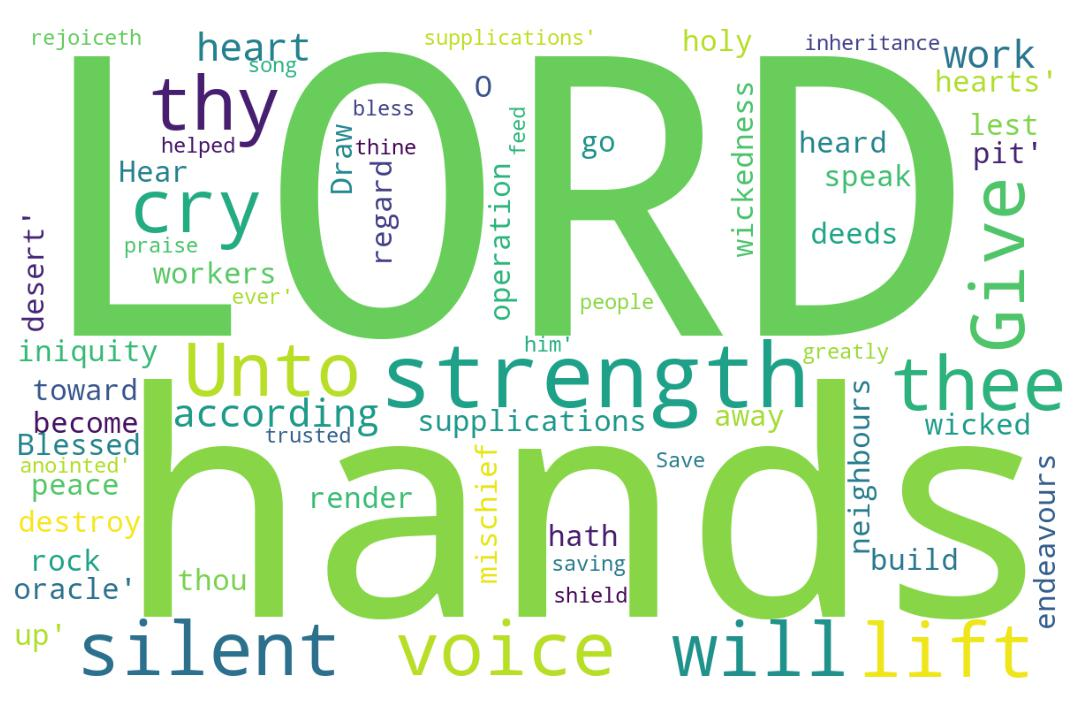
\includegraphics[width=\linewidth]{19OT-Psalms/Psalm28-WordCloud.jpg}
  \caption{Psalm 28 Word Cloud}
  \label{fig:Psalm 28 word Cloud}
\end{figure}

\marginpar{\scriptsize \centering \fcolorbox{bone}{lime}{\textbf{A VERY PERSONL FAITH}}\\ (Psalm  28:1--14) \begin{compactenum}[I.][8]
    \item His \textbf{Supplications} \index[scripture]{Psalms!Psa 028:02}\index[scripture]{Psalms!Psa 028:06}(Psa 28:2, 6)
    \item His \textbf{Surety} \index[scripture]{Psalms!Psa 028:05}(Psa 28:5)
    \item His \textbf{Song} \index[scripture]{Psalms!Psa 028:07}(Psa 28:7)
    \item His \textbf{Strength} \index[scripture]{Psalms!Psa 028:07}\index[scripture]{Psalms!Psa 028:08}(Psa 28:7, 8)
    \item His \textbf{Shield} \index[scripture]{Psalms!Psa 028:07}(Psa 28:7)
    \item His \textbf{Source} of Rejoicing \index[scripture]{Psalms!Psa 028:07}(Psa 28:7)
    \item His \textbf{Salvation} \index[scripture]{Psalms!Psa 028:08}\index[scripture]{Psalms!Psa 028:09}(Psa 28:8, 9)
\end{compactenum}}

\footnote{\textcolor[cmyk]{0.99998,1,0,0}{\hyperlink{TOC}{Return to end of Table of Contents.}}}\footnote{\href{https://www.audioverse.org/english/audiobibles/books/ENGKJV/O/Ps/1}{\textcolor[cmyk]{0.99998,1,0,0}{Psalms Audio}}}\textcolor[cmyk]{0.99998,1,0,0}{\emph{A Psalm} of David.}\\
\\
\textcolor[cmyk]{0.99998,1,0,0}{Unto thee will I cry, O LORD my rock; be not silent to me: lest, \emph{if} thou be silent to me, I become like them that go down into the pit.}\footnote{Study all the verses that contain the words \textbf{go}, \textbf{down}, and \textbf{pit}. The pit is literally the \textbf{bottomless pit} named in (1) Revelation 9:1, (2) Revelation 9:2, (3) Revelation 9:11, (4) Revelation 11:7, (5) Revelation 17:8, (6) Revelation 20:1, and (7) Revelation 20:3. It  is typified by the pit used to trap Joseph in Genesis 37.}
[2] \textcolor[cmyk]{0.99998,1,0,0}{Hear the voice of my \fcolorbox{bone}{lime}{supplications}, when I cry unto thee, when I lift up my hands toward thy holy oracle.}
[3] \textcolor[cmyk]{0.99998,1,0,0}{Draw me not away with the wicked, and with the workers of iniquity, which speak peace to their neighbours, but mischief \emph{is} in their hearts.}
[4] \textcolor[cmyk]{0.99998,1,0,0}{Give them according to their deeds, and according to the wickedness of their endeavours: give them after the work of their hands; render to them their desert.}
[5] \textcolor[cmyk]{0.99998,1,0,0}{Because they regard not the works of the LORD, nor the operation of his hands, \fcolorbox{bone}{lime}{he shall} destroy them, and not build them up.}
[6] \textcolor[cmyk]{0.99998,1,0,0}{Blessed \emph{be} the LORD, because he hath heard the voice of my supplications.}
[7] \textcolor[cmyk]{0.99998,1,0,0}{The LORD \emph{is} my \fcolorbox{bone}{lime}{strength} and my \fcolorbox{bone}{lime}{shield}; my heart trusted in him, and I am helped: therefore my heart greatly rejoiceth; and with my \fcolorbox{bone}{lime}{song} will I praise him.}
[8] \textcolor[cmyk]{0.99998,1,0,0}{The LORD \emph{is} their \fcolorbox{bone}{lime}{strength}, and he \emph{is} the saving \fcolorbox{bone}{lime}{strength} of his anointed.}
[9] \textcolor[cmyk]{0.99998,1,0,0}{\fcolorbox{bone}{lime}{Save} thy people, and bless thine inheritance: feed them also, and lift them up for ever.}




\section{Psalm 28 Comments}

\subsection{Numeric Nuggets}
The 13-letter word ``supplications'' is used twice in Psalm 28. There are 13 words in  verse 6.

\subsection{Introduction}
Phillips suggests that the Psalm may have been composed at at a time of  national crisis for Israel, specifically the period of civil war led by Absalom (2 Samuel 17-18). Verse 4 and 5 are imprecatory, calling for judgment against the evildoers, likely Ahithophel and his followers. The fact that Absalom was among this group was a source of immense distress given David's deep love for Absalom. Indeed, in the incident we see Absalom picturing rebellious Isreal rejecting God, seen in David. In Ahothophel, we see the great instigator himself, possibly referenced by ``the wicked'' in verse  3 (see cross references to ``wicked'' such as in Psalm 10). David also pictures the trusting remnant of Israel, redeemed in the end. The allusion is seen in the return of the plural pronouns in verses 8 and 9.  \cite{Phillips2001ExploringPsalms1} 

\subsection{Psalm 28:2}
An oracle is a thing or a place (in this case Jerusalem and the Temple), and oracles are the decrees that come from such. An example of the use of ``oracle'' can be seen in  2 Samuel 16:23.\footnote{\textbf{2 Samuel 16:23} - And the counsel of Ahithophel, which he counselled in those days, was as if a man had enquired at the oracle of God: so was all the counsel of Ahithophel both with David and with Absalom.} The oracles of God are described in Acts 7:38, Romans 3:2, Hebrews 5:12, and 1 Peter 4:11.\footnote{\textbf{Acts 7:38} - This is he, that was in the church in the wilderness with the angel which spake to him in the mount Sina, and with our fathers: who received the lively oracles to give unto us:}\footnote{\textbf{Romans 3:2} -  Much every way: chiefly, because that unto them were committed the oracles of God.}\footnote{\textbf{Hebrews 5:12} - or when for the time ye ought to be teachers, ye have need that one teach you again which be the first principles of the oracles of God; and are become such as have need of milk, and not of strong meat.}\footnote{\textbf{1 Peter 4:11} - If any man speak, let him speak as the oracles of God; if any man minister, let him do it as of the ability which God giveth: that God in all things may be glorified through Jesus Christ, to whom be praise and dominion for ever and ever. Amen.}

\subsection{Psalm 28:3}
Compare this prayer with that in Psalm 26:9.\footnote{\textbf{Psalm 26:9} - Gather not my soul with sinners, nor my life with bloody men:} 

\subsection{Psalm 28:8}
His ``anointed'' in the verse is a reference to David historically, and Jesus Christ doctrinally.\cite{Ruckman1992Psalms}

\subsection{Psalm 28:9}
There are four specific requests in verse 9, all aimed at the Jews:\cite{Ruckman1992Psalms}
\begin{compactenum}
	\item ``Save thy people'' (Romans 11:26)\footnote{\textbf{Romans 11:26} - And so all Israel shall be saved: as it is written, There shall come out of Sion the Deliverer, and shall turn away ungodliness from Jacob:}
	\item ``bless thin inheitance'' (Psalm 115:12)\footnote{\textbf{Psalm 115:12} - The LORD hath been mindful of us: he will bless us; he will bless the house of Israel; he will bless the house of Aaron.}\footnote{\textbf{Isaiah 2:6} - }
	\item ``feed them also'' (Ezekiel 34:14)\footnote{\textbf{Exekiel 34:14} - I will feed them in a good pasture, and upon the high mountains of Israel shall their fold be: there shall they lie in a good fold, and in a fat pasture shall they feed upon the mountains of Israel.}
	\item ``lift them up forever'' (Isaiah 65-66, Revelation 21-22)
\end{compactenum}

%\index[NWIV]{31!Psalms!Psa 28:1}\index[AWIP]{Unto!Psalms!Psa 28:1}\index[AWIP]{thee!Psalms!Psa 28:1}\index[AWIP]{will!Psalms!Psa 28:1}\index[AWIP]{I!Psalms!Psa 28:1}\index[AWIP]{I!Psalms!Psa 28:1 (2)}\index[AWIP]{cry!Psalms!Psa 28:1}\index[AWIP]{O!Psalms!Psa 28:1}\index[AWIP]{LORD!Psalms!Psa 28:1}\index[AWIP]{my!Psalms!Psa 28:1}\index[AWIP]{rock!Psalms!Psa 28:1}\index[AWIP]{be!Psalms!Psa 28:1}\index[AWIP]{be!Psalms!Psa 28:1 (2)}\index[AWIP]{not!Psalms!Psa 28:1}\index[AWIP]{silent!Psalms!Psa 28:1}\index[AWIP]{silent!Psalms!Psa 28:1 (2)}\index[AWIP]{to!Psalms!Psa 28:1}\index[AWIP]{to!Psalms!Psa 28:1 (2)}\index[AWIP]{me!Psalms!Psa 28:1}\index[AWIP]{me!Psalms!Psa 28:1 (2)}\index[AWIP]{lest!Psalms!Psa 28:1}\index[AWIP]{\emph{if}!Psalms!Psa 28:1}\index[AWIP]{thou!Psalms!Psa 28:1}\index[AWIP]{become!Psalms!Psa 28:1}\index[AWIP]{like!Psalms!Psa 28:1}\index[AWIP]{them!Psalms!Psa 28:1}\index[AWIP]{that!Psalms!Psa 28:1}\index[AWIP]{go!Psalms!Psa 28:1}\index[AWIP]{down!Psalms!Psa 28:1}\index[AWIP]{into!Psalms!Psa 28:1}\index[AWIP]{the!Psalms!Psa 28:1}\index[AWIP]{pit!Psalms!Psa 28:1}\index[AWIP]{\emph{if}!Psalms!Psa 28:1}

\index[NWIV]{21!Psalms!Psa 28:2}\index[AWIP]{Hear!Psalms!Psa 28:2}\index[AWIP]{the!Psalms!Psa 28:2}\index[AWIP]{voice!Psalms!Psa 28:2}\index[AWIP]{of!Psalms!Psa 28:2}\index[AWIP]{my!Psalms!Psa 28:2}\index[AWIP]{my!Psalms!Psa 28:2 (2)}\index[AWIP]{supplications!Psalms!Psa 28:2}\index[AWIP]{when!Psalms!Psa 28:2}\index[AWIP]{when!Psalms!Psa 28:2 (2)}\index[AWIP]{I!Psalms!Psa 28:2}\index[AWIP]{I!Psalms!Psa 28:2 (2)}\index[AWIP]{cry!Psalms!Psa 28:2}\index[AWIP]{unto!Psalms!Psa 28:2}\index[AWIP]{thee!Psalms!Psa 28:2}\index[AWIP]{lift!Psalms!Psa 28:2}\index[AWIP]{up!Psalms!Psa 28:2}\index[AWIP]{hands!Psalms!Psa 28:2}\index[AWIP]{toward!Psalms!Psa 28:2}\index[AWIP]{thy!Psalms!Psa 28:2}\index[AWIP]{holy!Psalms!Psa 28:2}\index[AWIP]{oracle!Psalms!Psa 28:2}

\index[NWIV]{25!Psalms!Psa 28:3}\index[AWIP]{Draw!Psalms!Psa 28:3}\index[AWIP]{me!Psalms!Psa 28:3}\index[AWIP]{not!Psalms!Psa 28:3}\index[AWIP]{away!Psalms!Psa 28:3}\index[AWIP]{with!Psalms!Psa 28:3}\index[AWIP]{with!Psalms!Psa 28:3 (2)}\index[AWIP]{the!Psalms!Psa 28:3}\index[AWIP]{the!Psalms!Psa 28:3 (2)}\index[AWIP]{wicked!Psalms!Psa 28:3}\index[AWIP]{and!Psalms!Psa 28:3}\index[AWIP]{workers!Psalms!Psa 28:3}\index[AWIP]{of!Psalms!Psa 28:3}\index[AWIP]{iniquity!Psalms!Psa 28:3}\index[AWIP]{which!Psalms!Psa 28:3}\index[AWIP]{speak!Psalms!Psa 28:3}\index[AWIP]{peace!Psalms!Psa 28:3}\index[AWIP]{to!Psalms!Psa 28:3}\index[AWIP]{their!Psalms!Psa 28:3}\index[AWIP]{their!Psalms!Psa 28:3 (2)}\index[AWIP]{neighbours!Psalms!Psa 28:3}\index[AWIP]{but!Psalms!Psa 28:3}\index[AWIP]{mischief!Psalms!Psa 28:3}\index[AWIP]{\emph{is}!Psalms!Psa 28:3}\index[AWIP]{in!Psalms!Psa 28:3}\index[AWIP]{hearts!Psalms!Psa 28:3}\index[AWIP]{\emph{is}!Psalms!Psa 28:3}

\index[NWIV]{27!Psalms!Psa 28:4}\index[AWIP]{Give!Psalms!Psa 28:4}\index[AWIP]{them!Psalms!Psa 28:4}\index[AWIP]{them!Psalms!Psa 28:4 (2)}\index[AWIP]{them!Psalms!Psa 28:4 (3)}\index[AWIP]{according!Psalms!Psa 28:4}\index[AWIP]{according!Psalms!Psa 28:4 (2)}\index[AWIP]{to!Psalms!Psa 28:4}\index[AWIP]{to!Psalms!Psa 28:4 (2)}\index[AWIP]{to!Psalms!Psa 28:4 (3)}\index[AWIP]{their!Psalms!Psa 28:4}\index[AWIP]{their!Psalms!Psa 28:4 (2)}\index[AWIP]{their!Psalms!Psa 28:4 (3)}\index[AWIP]{their!Psalms!Psa 28:4 (4)}\index[AWIP]{deeds!Psalms!Psa 28:4}\index[AWIP]{and!Psalms!Psa 28:4}\index[AWIP]{the!Psalms!Psa 28:4}\index[AWIP]{the!Psalms!Psa 28:4 (2)}\index[AWIP]{wickedness!Psalms!Psa 28:4}\index[AWIP]{of!Psalms!Psa 28:4}\index[AWIP]{of!Psalms!Psa 28:4 (2)}\index[AWIP]{endeavours!Psalms!Psa 28:4}\index[AWIP]{give!Psalms!Psa 28:4}\index[AWIP]{after!Psalms!Psa 28:4}\index[AWIP]{work!Psalms!Psa 28:4}\index[AWIP]{hands!Psalms!Psa 28:4}\index[AWIP]{render!Psalms!Psa 28:4}\index[AWIP]{desert!Psalms!Psa 28:4}

\index[NWIV]{24!Psalms!Psa 28:5}\index[AWIP]{Because!Psalms!Psa 28:5}\index[AWIP]{they!Psalms!Psa 28:5}\index[AWIP]{regard!Psalms!Psa 28:5}\index[AWIP]{not!Psalms!Psa 28:5}\index[AWIP]{not!Psalms!Psa 28:5 (2)}\index[AWIP]{the!Psalms!Psa 28:5}\index[AWIP]{the!Psalms!Psa 28:5 (2)}\index[AWIP]{the!Psalms!Psa 28:5 (3)}\index[AWIP]{works!Psalms!Psa 28:5}\index[AWIP]{of!Psalms!Psa 28:5}\index[AWIP]{of!Psalms!Psa 28:5 (2)}\index[AWIP]{LORD!Psalms!Psa 28:5}\index[AWIP]{nor!Psalms!Psa 28:5}\index[AWIP]{operation!Psalms!Psa 28:5}\index[AWIP]{his!Psalms!Psa 28:5}\index[AWIP]{hands!Psalms!Psa 28:5}\index[AWIP]{he!Psalms!Psa 28:5}\index[AWIP]{shall!Psalms!Psa 28:5}\index[AWIP]{destroy!Psalms!Psa 28:5}\index[AWIP]{them!Psalms!Psa 28:5}\index[AWIP]{them!Psalms!Psa 28:5 (2)}\index[AWIP]{and!Psalms!Psa 28:5}\index[AWIP]{build!Psalms!Psa 28:5}\index[AWIP]{up!Psalms!Psa 28:5}

\index[NWIV]{13!Psalms!Psa 28:6}\index[AWIP]{Blessed!Psalms!Psa 28:6}\index[AWIP]{\emph{be}!Psalms!Psa 28:6}\index[AWIP]{the!Psalms!Psa 28:6}\index[AWIP]{the!Psalms!Psa 28:6 (2)}\index[AWIP]{LORD!Psalms!Psa 28:6}\index[AWIP]{because!Psalms!Psa 28:6}\index[AWIP]{he!Psalms!Psa 28:6}\index[AWIP]{hath!Psalms!Psa 28:6}\index[AWIP]{heard!Psalms!Psa 28:6}\index[AWIP]{voice!Psalms!Psa 28:6}\index[AWIP]{of!Psalms!Psa 28:6}\index[AWIP]{my!Psalms!Psa 28:6}\index[AWIP]{supplications!Psalms!Psa 28:6}\index[AWIP]{\emph{be}!Psalms!Psa 28:6}

\index[NWIV]{30!Psalms!Psa 28:7}\index[AWIP]{The!Psalms!Psa 28:7}\index[AWIP]{LORD!Psalms!Psa 28:7}\index[AWIP]{\emph{is}!Psalms!Psa 28:7}\index[AWIP]{my!Psalms!Psa 28:7}\index[AWIP]{my!Psalms!Psa 28:7 (2)}\index[AWIP]{my!Psalms!Psa 28:7 (3)}\index[AWIP]{my!Psalms!Psa 28:7 (4)}\index[AWIP]{my!Psalms!Psa 28:7 (5)}\index[AWIP]{strength!Psalms!Psa 28:7}\index[AWIP]{and!Psalms!Psa 28:7}\index[AWIP]{and!Psalms!Psa 28:7 (2)}\index[AWIP]{and!Psalms!Psa 28:7 (3)}\index[AWIP]{shield!Psalms!Psa 28:7}\index[AWIP]{heart!Psalms!Psa 28:7}\index[AWIP]{heart!Psalms!Psa 28:7 (2)}\index[AWIP]{trusted!Psalms!Psa 28:7}\index[AWIP]{in!Psalms!Psa 28:7}\index[AWIP]{him!Psalms!Psa 28:7}\index[AWIP]{him!Psalms!Psa 28:7 (2)}\index[AWIP]{I!Psalms!Psa 28:7}\index[AWIP]{I!Psalms!Psa 28:7 (2)}\index[AWIP]{am!Psalms!Psa 28:7}\index[AWIP]{helped!Psalms!Psa 28:7}\index[AWIP]{therefore!Psalms!Psa 28:7}\index[AWIP]{greatly!Psalms!Psa 28:7}\index[AWIP]{rejoiceth!Psalms!Psa 28:7}\index[AWIP]{with!Psalms!Psa 28:7}\index[AWIP]{song!Psalms!Psa 28:7}\index[AWIP]{will!Psalms!Psa 28:7}\index[AWIP]{praise!Psalms!Psa 28:7}\index[AWIP]{\emph{is}!Psalms!Psa 28:7}

\index[NWIV]{14!Psalms!Psa 28:8}\index[AWIP]{The!Psalms!Psa 28:8}\index[AWIP]{LORD!Psalms!Psa 28:8}\index[AWIP]{\emph{is}!Psalms!Psa 28:8}\index[AWIP]{\emph{is}!Psalms!Psa 28:8 (2)}\index[AWIP]{their!Psalms!Psa 28:8}\index[AWIP]{strength!Psalms!Psa 28:8}\index[AWIP]{strength!Psalms!Psa 28:8 (2)}\index[AWIP]{and!Psalms!Psa 28:8}\index[AWIP]{he!Psalms!Psa 28:8}\index[AWIP]{the!Psalms!Psa 28:8}\index[AWIP]{saving!Psalms!Psa 28:8}\index[AWIP]{of!Psalms!Psa 28:8}\index[AWIP]{his!Psalms!Psa 28:8}\index[AWIP]{anointed!Psalms!Psa 28:8}\index[AWIP]{\emph{is}!Psalms!Psa 28:8}\index[AWIP]{\emph{is}!Psalms!Psa 28:8 (2)}

\index[NWIV]{16!Psalms!Psa 28:9}\index[AWIP]{Save!Psalms!Psa 28:9}\index[AWIP]{thy!Psalms!Psa 28:9}\index[AWIP]{people!Psalms!Psa 28:9}\index[AWIP]{and!Psalms!Psa 28:9}\index[AWIP]{and!Psalms!Psa 28:9 (2)}\index[AWIP]{bless!Psalms!Psa 28:9}\index[AWIP]{thine!Psalms!Psa 28:9}\index[AWIP]{inheritance!Psalms!Psa 28:9}\index[AWIP]{feed!Psalms!Psa 28:9}\index[AWIP]{them!Psalms!Psa 28:9}\index[AWIP]{them!Psalms!Psa 28:9 (2)}\index[AWIP]{also!Psalms!Psa 28:9}\index[AWIP]{lift!Psalms!Psa 28:9}\index[AWIP]{up!Psalms!Psa 28:9}\index[AWIP]{for!Psalms!Psa 28:9}\index[AWIP]{ever!Psalms!Psa 28:9}


\section{Psalm 28 Outlines}

\subsection{My Outlines}

\subsubsection{David's Very Personal Faith}
%\textbf{Introduction:} Psalm 28:\footnote{04 July 2016, Keith Anthony.}
\index[speaker]{Keith Anthony!Psalm 28 (David's Very Personal Faith)}
\index[series]{Psalms (Keith Anthony)!Psalm 28 (David's Very Personal Faith)}
\index[date]{2016/07/04!Psalm 28 (David's Very Personal Faith) (Keith Anthony)}
\begin{compactenum}[I.]
    \item His \textbf{Supplications} \index[scripture]{Psalms!Psa 028:02}\index[scripture]{Psalms!Psa 028:06}(Psa 28:2, 6)
    \item His \textbf{Surety} \index[scripture]{Psalms!Psa 028:05}(Psa 28:5)
    \item His \textbf{Song} \index[scripture]{Psalms!Psa 028:07}(Psa 28:7)
    \item His \textbf{Strength} \index[scripture]{Psalms!Psa 028:07}\index[scripture]{Psalms!Psa 028:08}(Psa 28:7, 8)
    \item His \textbf{Shield} \index[scripture]{Psalms!Psa 028:07}(Psa 28:7)
    \item His \textbf{Source} of Rejoicing \index[scripture]{Psalms!Psa 028:07}(Psa 28:7)
    \item His \textbf{Salvation} \index[scripture]{Psalms!Psa 028:08}\index[scripture]{Psalms!Psa 028:09}(Psa 28:8, 9)
\end{compactenum}

%Psalm 28 Clark Herring, 10/23/18, Fundamental Baptist Sermon Outlines
%“What to Remember in the Silent Times”
%I. Remember to Recognize the Rock (vs1-2)
%A) The Distinction of the Rock (vs1a) (my)
%B) The Description of the Rock (vs1b) (Rock)
%C) The Dependence on the Rock (vs1c)
%D) The Devotion to the Rock (vs2)
%II. Remember the Results of the Rebellious (vs3-5)
%A) Their Luring (vs3)
%B) Their Labor (vs4)
%C) Their Leader (vs5)
%III. Remember to Rejoice with the Righteous (vs6-9)
%A) The Attention of our Lord (vs6)
%B) The Attributes of our Lord (vs7-8)
%C) The Abilities of our Lord (vs9)
%a) to Save
%b) to Satisfy
%c) to Sustain
%d) to Supply
%e) to Strengthen

%Psalm 28 Clarence Billheimer, 1/22/20, Fundamental Baptist Sermon Outlines
%Introduction: Silence is an eerie thing. You know how you feel when you’re talking to someone and they sit there silent, appearing as though they’re not listening to you. You know how frustrating it is to call for someone and no one answers. Imagine what it can be like when God appears to be silent! After all, He’s omniscient, omnipresent, and omnipotent. He’s able to hear millions of voices at one and not be confused. He can respond to cries instantly and many at once. In Psalm 28 there’s a prayer of David he may have prayed while being pursued by Saul or some other enemy. Believe me, when we’re in trouble of any kind, that’s not the time we want to feel God is silent! Let’s follow the progression of this experience in David’s life to see the Lord was not silent at all.
%I. The cry (28:1, 2)
%A. To a strong source
%B. With a spoken supplication
%C. Toward a specific spot
%D. Because of a potential sad slide
%II. The condemnation (28:3-5)
%A. The wicked and workers of iniquity are deceitful.
%B. The wicked and workers of iniquity are doomed.
%C. The wicked and workers of iniquity will be destroyed.
%III. The chorus (28:6-9)
%A. God has heard.
%B. Man’s heart has trusted and been helped.
%C. Man’s response is heralded.
%D. God’s abilities are echoed toward others.
%Conclusion: The final verse closes this prayer of David with a plea that God will do for others what He had just done for David. That should be our prayer when we experience the hearing of God and answer to prayer.
\subsection{Outlines from Others}


%\section{Psalm 28 Statistics}

%%%%%%%%%%%%%%%%%%%%%%%%%%%
%%%%% Word Statistics
%%%%%%%%%%%%%%%%%%%%%%%%%%


\normalsize



\subsection{Chapter Word Statistics}


%%%%%%%%%%
%%%%%%%%%%
 
\begin{center}
\begin{longtable}{l|c|c|c|c}
\caption[Stats for Psalm 28]{Stats for Psalm 28} \label{table:Stats for Psalm 28} \\ 
\hline \multicolumn{1}{|c|}{\textbf{Verse(s)}} & \multicolumn{1}{|c|}{\textbf{Count}} & \multicolumn{1}{|c|}{\textbf{Unique}} & \multicolumn{1}{|c|}{\textbf{Italics}} & \multicolumn{1}{|c|}{\textbf{Uniq Italic}}  \\ \hline 
\endfirsthead
 
\multicolumn{5}{c}
{{\bfseries \tablename\ \thetable{} -- continued from previous page}} \\  
\hline \multicolumn{1}{|c|}{\textbf{Verse(s)}} & \multicolumn{1}{|c|}{\textbf{Count}} & \multicolumn{1}{|c|}{\textbf{Unique}} & \multicolumn{1}{|c|}{\textbf{Italics}} & \multicolumn{1}{|c|}{\textbf{Uniq Italic}}  \\ \hline 
\endhead
 
\hline \multicolumn{5}{|r|}{{Continued if needed}} \\ \hline
\endfoot 
1 & 31 & 26 & 1 & 1\\ \hline
2 & 21 & 18 & 0 & 0\\ \hline
3 & 25 & 22 & 1 & 1\\ \hline
4 & 27 & 17 & 0 & 0\\ \hline
5 & 24 & 19 & 0 & 0\\ \hline
6 & 13 & 12 & 1 & 1\\ \hline
7 & 30 & 21 & 1 & 1\\ \hline
8 & 14 & 12 & 2 & 1\\ \hline
9 & 16 & 14 & 0 & 0\\ \hline
\hline \hline
Total & 201 & 106 & 6 & 3



\end{longtable}
\end{center}

%%%%%%%%%%
%%%%%%%%%%
 
\subsection{Words by Frequency}

\begin{center}
\begin{longtable}{l|r}
\caption[Word Frequencies in Psalm 28]{Word Frequencies in Psalm 28} \label{table:WordsIn-Psalm-28} \\ 
\hline \multicolumn{1}{|c|}{\textbf{Word}} & \multicolumn{1}{c|}{\textbf{Frequency}} \\ \hline 
\endfirsthead
 
\multicolumn{2}{c}
{{\bfseries \tablename\ \thetable{} -- continued from previous page}} \\ 
\hline \multicolumn{1}{|c|}{\textbf{Word}} & \multicolumn{1}{c|}{\textbf{Frequency}} \\ \hline 
\endhead
 
\hline \multicolumn{2}{|r|}{{Continued if needed}} \\ \hline
\endfoot
 
\hline \hline
\endlastfoot
the & 12 \\ \hline
my & 9 \\ \hline
and & 9 \\ \hline
them & 8 \\ \hline
of & 8 \\ \hline
their & 7 \\ \hline
I & 6 \\ \hline
to & 6 \\ \hline
LORD & 5 \\ \hline
not & 4 \\ \hline
\emph{is} & 4 \\ \hline
me & 3 \\ \hline
up & 3 \\ \hline
hands & 3 \\ \hline
with & 3 \\ \hline
he & 3 \\ \hline
strength & 3 \\ \hline
thee & 2 \\ \hline
will & 2 \\ \hline
cry & 2 \\ \hline
be & 2 \\ \hline
silent & 2 \\ \hline
voice & 2 \\ \hline
supplications & 2 \\ \hline
when & 2 \\ \hline
lift & 2 \\ \hline
thy & 2 \\ \hline
in & 2 \\ \hline
according & 2 \\ \hline
his & 2 \\ \hline
The & 2 \\ \hline
heart & 2 \\ \hline
him & 2 \\ \hline
Unto & 1 \\ \hline
O & 1 \\ \hline
rock & 1 \\ \hline
lest & 1 \\ \hline
\emph{if} & 1 \\ \hline
thou & 1 \\ \hline
become & 1 \\ \hline
like & 1 \\ \hline
that & 1 \\ \hline
go & 1 \\ \hline
down & 1 \\ \hline
into & 1 \\ \hline
pit & 1 \\ \hline
Hear & 1 \\ \hline
unto & 1 \\ \hline
toward & 1 \\ \hline
holy & 1 \\ \hline
oracle & 1 \\ \hline
Draw & 1 \\ \hline
away & 1 \\ \hline
wicked & 1 \\ \hline
workers & 1 \\ \hline
iniquity & 1 \\ \hline
which & 1 \\ \hline
speak & 1 \\ \hline
peace & 1 \\ \hline
neighbours & 1 \\ \hline
but & 1 \\ \hline
mischief & 1 \\ \hline
hearts & 1 \\ \hline
Give & 1 \\ \hline
deeds & 1 \\ \hline
wickedness & 1 \\ \hline
endeavours & 1 \\ \hline
give & 1 \\ \hline
after & 1 \\ \hline
work & 1 \\ \hline
render & 1 \\ \hline
desert & 1 \\ \hline
Because & 1 \\ \hline
they & 1 \\ \hline
regard & 1 \\ \hline
works & 1 \\ \hline
nor & 1 \\ \hline
operation & 1 \\ \hline
shall & 1 \\ \hline
destroy & 1 \\ \hline
build & 1 \\ \hline
Blessed & 1 \\ \hline
\emph{be} & 1 \\ \hline
because & 1 \\ \hline
hath & 1 \\ \hline
heard & 1 \\ \hline
shield & 1 \\ \hline
trusted & 1 \\ \hline
am & 1 \\ \hline
helped & 1 \\ \hline
therefore & 1 \\ \hline
greatly & 1 \\ \hline
rejoiceth & 1 \\ \hline
song & 1 \\ \hline
praise & 1 \\ \hline
saving & 1 \\ \hline
anointed & 1 \\ \hline
Save & 1 \\ \hline
people & 1 \\ \hline
bless & 1 \\ \hline
thine & 1 \\ \hline
inheritance & 1 \\ \hline
feed & 1 \\ \hline
also & 1 \\ \hline
for & 1 \\ \hline
ever & 1 \\ \hline
\end{longtable}
\end{center}



\normalsize



\subsection{Words Alphabetically}

\begin{center}
\begin{longtable}{l|r}
\caption[Word Alphabetically in Psalm 28]{Word Alphabetically in Psalm 28} \label{table:WordsIn-Psalm-28} \\ 
\hline \multicolumn{1}{|c|}{\textbf{Word}} & \multicolumn{1}{c|}{\textbf{Frequency}} \\ \hline 
\endfirsthead
 
\multicolumn{2}{c}
{{\bfseries \tablename\ \thetable{} -- continued from previous page}} \\ 
\hline \multicolumn{1}{|c|}{\textbf{Word}} & \multicolumn{1}{c|}{\textbf{Frequency}} \\ \hline 
\endhead
 
\hline \multicolumn{2}{|r|}{{Continued if needed}} \\ \hline
\endfoot
 
\hline \hline
\endlastfoot
Because & 1 \\ \hline
Blessed & 1 \\ \hline
Draw & 1 \\ \hline
Give & 1 \\ \hline
Hear & 1 \\ \hline
I & 6 \\ \hline
LORD & 5 \\ \hline
O & 1 \\ \hline
Save & 1 \\ \hline
The & 2 \\ \hline
Unto & 1 \\ \hline
\emph{be} & 1 \\ \hline
\emph{if} & 1 \\ \hline
\emph{is} & 4 \\ \hline
according & 2 \\ \hline
after & 1 \\ \hline
also & 1 \\ \hline
am & 1 \\ \hline
and & 9 \\ \hline
anointed & 1 \\ \hline
away & 1 \\ \hline
be & 2 \\ \hline
because & 1 \\ \hline
become & 1 \\ \hline
bless & 1 \\ \hline
build & 1 \\ \hline
but & 1 \\ \hline
cry & 2 \\ \hline
deeds & 1 \\ \hline
desert & 1 \\ \hline
destroy & 1 \\ \hline
down & 1 \\ \hline
endeavours & 1 \\ \hline
ever & 1 \\ \hline
feed & 1 \\ \hline
for & 1 \\ \hline
give & 1 \\ \hline
go & 1 \\ \hline
greatly & 1 \\ \hline
hands & 3 \\ \hline
hath & 1 \\ \hline
he & 3 \\ \hline
heard & 1 \\ \hline
heart & 2 \\ \hline
hearts & 1 \\ \hline
helped & 1 \\ \hline
him & 2 \\ \hline
his & 2 \\ \hline
holy & 1 \\ \hline
in & 2 \\ \hline
inheritance & 1 \\ \hline
iniquity & 1 \\ \hline
into & 1 \\ \hline
lest & 1 \\ \hline
lift & 2 \\ \hline
like & 1 \\ \hline
me & 3 \\ \hline
mischief & 1 \\ \hline
my & 9 \\ \hline
neighbours & 1 \\ \hline
nor & 1 \\ \hline
not & 4 \\ \hline
of & 8 \\ \hline
operation & 1 \\ \hline
oracle & 1 \\ \hline
peace & 1 \\ \hline
people & 1 \\ \hline
pit & 1 \\ \hline
praise & 1 \\ \hline
regard & 1 \\ \hline
rejoiceth & 1 \\ \hline
render & 1 \\ \hline
rock & 1 \\ \hline
saving & 1 \\ \hline
shall & 1 \\ \hline
shield & 1 \\ \hline
silent & 2 \\ \hline
song & 1 \\ \hline
speak & 1 \\ \hline
strength & 3 \\ \hline
supplications & 2 \\ \hline
that & 1 \\ \hline
the & 12 \\ \hline
thee & 2 \\ \hline
their & 7 \\ \hline
them & 8 \\ \hline
therefore & 1 \\ \hline
they & 1 \\ \hline
thine & 1 \\ \hline
thou & 1 \\ \hline
thy & 2 \\ \hline
to & 6 \\ \hline
toward & 1 \\ \hline
trusted & 1 \\ \hline
unto & 1 \\ \hline
up & 3 \\ \hline
voice & 2 \\ \hline
when & 2 \\ \hline
which & 1 \\ \hline
wicked & 1 \\ \hline
wickedness & 1 \\ \hline
will & 2 \\ \hline
with & 3 \\ \hline
work & 1 \\ \hline
workers & 1 \\ \hline
works & 1 \\ \hline
\end{longtable}
\end{center}



\normalsize



\subsection{Word Lengths in Chapter}
\normalsize
\begin{longtable}{l|p{3.75in}}
\caption[Words by Length in Psalm 28]{Words by Length in Psalm 28} \label{table:WordsIn-Psalm-28} \\ 
\hline \multicolumn{1}{|c|}{\textbf{Length}} & \multicolumn{1}{c|}{\textbf{Words}} \\ \hline 
\endfirsthead
 
\multicolumn{2}{c}
{{\bfseries \tablename\ \thetable{} -- continued from previous page}} \\ 
\hline \multicolumn{1}{|c|}{\textbf{Length}} & \multicolumn{1}{c|}{\textbf{Words}} \\ \hline 
\endhead
 
\hline \multicolumn{2}{|r|}{{Continued if needed}} \\ \hline
\endfoot
 
\hline \hline
\endlastfoot
1 & I, O \\ \hline
2 & my, be, to, me, \emph{if}, go, of, up, \emph{is}, in, he, \emph{be}, am \\ \hline
3 & cry, not, the, pit, thy, and, but, nor, his, The, him, for \\ \hline
4 & Unto, thee, will, LORD, rock, lest, thou, like, them, that, down, into, Hear, when, unto, lift, holy, Draw, away, with, Give, give, work, they, hath, song, Save, feed, also, ever \\ \hline
5 & voice, hands, which, speak, peace, their, deeds, after, works, shall, build, heard, heart, bless, thine \\ \hline
6 & silent, become, toward, oracle, wicked, hearts, render, desert, regard, shield, helped, praise, saving, people \\ \hline
7 & workers, Because, destroy, Blessed, because, trusted, greatly \\ \hline
8 & iniquity, mischief, strength, anointed \\ \hline
9 & according, operation, therefore, rejoiceth \\ \hline
10 & neighbours, wickedness, endeavours \\ \hline
11 & inheritance \\ \hline
13 & supplications \\ \hline
\end{longtable}






%%%%%%%%%%
%%%%%%%%%%
 



%%%%%%%%%%
%%%%%%%%%%
\subsection{Verses with 13 Words in Chapter}
\normalsize
\begin{longtable}{l|p{3.75in}}
\caption[Verses with 13 Words  in Psalm 28]{Verses with 13 Words  in Psalm 28} \label{table:Verses with 13 Words in-Psalm-28} \\ 
\hline \multicolumn{1}{|c|}{\textbf{Reference}} & \multicolumn{1}{c|}{\textbf{Verse}} \\ \hline 
\endfirsthead
 
\multicolumn{2}{c}
{{\bfseries \tablename\ \thetable{} -- continued from previous page}} \\ 
\hline \multicolumn{1}{|c|}{\textbf{Reference}} & \multicolumn{1}{c|}{\textbf{Verse}} \\ \hline 
\endhead
 
\hline \multicolumn{2}{|r|}{{Continued if needed}} \\ \hline
\endfoot
 
\hline \hline
\endlastfoot
Psalms 028:6 & Blessed \emph{be} the LORD, because he hath heard the voice of my supplications. \\ \hline
\end{longtable}






%%%%%%%%%%
%%%%%%%%%%
\subsection{Psalm 28 Repeated Phrases}


%%%%%%%%%%
%%%%%%%%%%
\normalsize
 
\begin{center}
\begin{longtable}{|p{3.0in}|p{0.5in}|}
\caption[Psalm 28 Repeated Phrases]{Psalm 28 Repeated Phrases}\label{table:Repeated Phrases Psalm 28} \\
\hline \multicolumn{1}{|c|}{\textbf{Phrase}} & \multicolumn{1}{c|}{\textbf{Frequency}} \\ \hline 
\endfirsthead
 
\multicolumn{2}{c}
{{\bfseries \tablename\ \thetable{} -- continued from previous page}} \\  
\hline \multicolumn{1}{|c|}{\textbf{Phrase}} & \multicolumn{1}{c|}{\textbf{Frequency}} \\ \hline 
\endhead
 
\hline \multicolumn{2}{c}{{ }} \\ \hline
\endfoot 
\end{longtable}
\end{center}



%%%%%%%%%%
%%%%%%%%%%




\chapter{Psalm 29}

\begin{figure}
  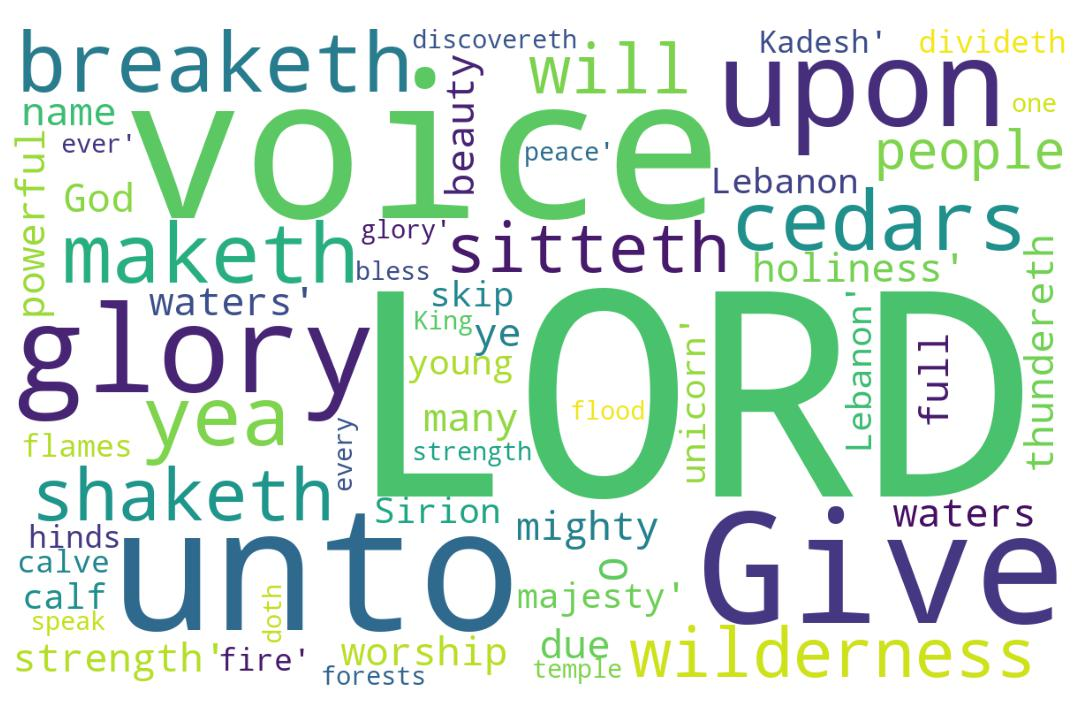
\includegraphics[width=\linewidth]{19OT-Psalms/Psalm29-WordCloud.jpg}
  \caption{Psalm 29 Word Cloud}
  \label{fig:Psalm 29 word Cloud}
\end{figure}


\marginpar{\scriptsize \centering \fcolorbox{bone}{lime}{\textbf{THE VOICE OF THE LORD}}\\ (Psalm 29:1-11) \begin{compactenum}[I.][8]
    \item \textbf{God's Place} \index[scripture]{Psalms!Psa 029:01}(Psa 29:1)
    \item \textbf{God's Presence Obvious} \index[scripture]{Psalms!Psa 029:03-09}(Psa 29:3-9)
    \item \textbf{God's Power Observed} \index[scripture]{Psalms!Psa 029:04}(Psa 29:4)
    \item \textbf{God's Peace Obtained} \index[scripture]{Psalms!Psa 029:11}(Psa 29:11)
    \item \textbf{God's People} \index[scripture]{Psalms!Psa 029:11}(Psa 29:11)
    \item \textbf{God's Preservation Ordained} \index[scripture]{Psalms!Psa 029:11}(Psa 29:11)
    \item \textbf{God's Providence}
\end{compactenum}}

\footnote{\textcolor[cmyk]{0.99998,1,0,0}{\hyperlink{TOC}{Return to end of Table of Contents.}}}\footnote{\href{https://audiobible.com/bible}{\textcolor[cmyk]{0.99998,1,0,0}{Psalms Audio}}}\textcolor[cmyk]{0.99998,1,0,0}{Give unto the LORD, O ye mighty, \fcolorbox{bone}{lime}{give unto the LORD} glory and strength.}
[2] \textcolor[cmyk]{0.99998,1,0,0}{Give unto the LORD the glory due unto his name; worship the LORD in the beauty of holiness.}
[3] \textcolor[cmyk]{0.99998,1,0,0}{The voice of the LORD \emph{is} upon the waters: the God of glory \fcolorbox{bone}{lime}{thundereth}: the LORD \emph{is} upon many waters.}
[4] \textcolor[cmyk]{0.99998,1,0,0}{The voice of the LORD \emph{is} \fcolorbox{bone}{lime}{powerful}; the voice of the LORD \emph{is} full of majesty.}
[5] \textcolor[cmyk]{0.99998,1,0,0}{The voice of the LORD breaketh the cedars; yea, the LORD breaketh the cedars of Lebanon.}
[6] \textcolor[cmyk]{0.99998,1,0,0}{He maketh them also to skip like a calf; Lebanon and Sirion like a young unicorn.}
[7] \textcolor[cmyk]{0.99998,1,0,0}{The voice of the LORD divideth the flames of fire.}
[8] \textcolor[cmyk]{0.99998,1,0,0}{The voice of the LORD shaketh the wilderness; the LORD shaketh the wilderness of Kadesh.}
[9] \textcolor[cmyk]{0.99998,1,0,0}{The voice of the LORD maketh the hinds to calve, and discovereth the forests: and in his temple doth every one speak of \emph{his} glory.}
[10] \textcolor[cmyk]{0.99998,1,0,0}{The LORD sitteth upon the flood; yea, the LORD sitteth King for ever.}
[11] \textcolor[cmyk]{0.99998,1,0,0}{The LORD will give strength unto his \fcolorbox{bone}{lime}{people}; the LORD will bless his people with \fcolorbox{bone}{lime}{peace}.}



\section{Psalm 29 Comments}

\subsection{Numeric Nuggets}
\textbf{16: } The phrase ``the LORD'' is used 16 times in the psalm.  I have the number 16 as the number of witness (4 * 4).\\
\noindent \textbf{13:} There are 13 words in Psalm 29:10. There are 13 unique words in verse 2. \\
\noindent \textbf{7: } The phrase ``voice of the LORD'' is found 7 times.\\
\\
\noindent Verse 10 has 13 words. Verse 2 has 13 unique words.

\subsection{Introduction}
Compare with Psalm 1. Here David walks in integrity (Psalm 26:1), stands in an even place (Psalm 26:12), and does not sit with vain persons or evil doer (Psalm 26:4, 5).

%\index[NWIV]{14!Psalms!Psa 29:1}\index[AWIP]{Give!Psalms!Psa 29:1}\index[AWIP]{unto!Psalms!Psa 29:1}\index[AWIP]{unto!Psalms!Psa 29:1 (2)}\index[AWIP]{the!Psalms!Psa 29:1}\index[AWIP]{the!Psalms!Psa 29:1 (2)}\index[AWIP]{LORD!Psalms!Psa 29:1}\index[AWIP]{LORD!Psalms!Psa 29:1 (2)}\index[AWIP]{O!Psalms!Psa 29:1}\index[AWIP]{ye!Psalms!Psa 29:1}\index[AWIP]{mighty!Psalms!Psa 29:1}\index[AWIP]{give!Psalms!Psa 29:1}\index[AWIP]{glory!Psalms!Psa 29:1}\index[AWIP]{and!Psalms!Psa 29:1}\index[AWIP]{strength!Psalms!Psa 29:1}

\index[NWIV]{18!Psalms!Psa 29:2}\index[AWIP]{Give!Psalms!Psa 29:2}\index[AWIP]{unto!Psalms!Psa 29:2}\index[AWIP]{unto!Psalms!Psa 29:2 (2)}\index[AWIP]{the!Psalms!Psa 29:2}\index[AWIP]{the!Psalms!Psa 29:2 (2)}\index[AWIP]{the!Psalms!Psa 29:2 (3)}\index[AWIP]{the!Psalms!Psa 29:2 (4)}\index[AWIP]{LORD!Psalms!Psa 29:2}\index[AWIP]{LORD!Psalms!Psa 29:2 (2)}\index[AWIP]{glory!Psalms!Psa 29:2}\index[AWIP]{due!Psalms!Psa 29:2}\index[AWIP]{his!Psalms!Psa 29:2}\index[AWIP]{name!Psalms!Psa 29:2}\index[AWIP]{worship!Psalms!Psa 29:2}\index[AWIP]{in!Psalms!Psa 29:2}\index[AWIP]{beauty!Psalms!Psa 29:2}\index[AWIP]{of!Psalms!Psa 29:2}\index[AWIP]{holiness!Psalms!Psa 29:2}

\index[NWIV]{20!Psalms!Psa 29:3}\index[AWIP]{The!Psalms!Psa 29:3}\index[AWIP]{voice!Psalms!Psa 29:3}\index[AWIP]{of!Psalms!Psa 29:3}\index[AWIP]{of!Psalms!Psa 29:3 (2)}\index[AWIP]{the!Psalms!Psa 29:3}\index[AWIP]{the!Psalms!Psa 29:3 (2)}\index[AWIP]{the!Psalms!Psa 29:3 (3)}\index[AWIP]{the!Psalms!Psa 29:3 (4)}\index[AWIP]{LORD!Psalms!Psa 29:3}\index[AWIP]{LORD!Psalms!Psa 29:3 (2)}\index[AWIP]{\emph{is}!Psalms!Psa 29:3}\index[AWIP]{\emph{is}!Psalms!Psa 29:3 (2)}\index[AWIP]{upon!Psalms!Psa 29:3}\index[AWIP]{upon!Psalms!Psa 29:3 (2)}\index[AWIP]{waters!Psalms!Psa 29:3}\index[AWIP]{waters!Psalms!Psa 29:3 (2)}\index[AWIP]{God!Psalms!Psa 29:3}\index[AWIP]{glory!Psalms!Psa 29:3}\index[AWIP]{thundereth!Psalms!Psa 29:3}\index[AWIP]{many!Psalms!Psa 29:3}\index[AWIP]{\emph{is}!Psalms!Psa 29:3}\index[AWIP]{\emph{is}!Psalms!Psa 29:3 (2)}

\index[NWIV]{16!Psalms!Psa 29:4}\index[AWIP]{The!Psalms!Psa 29:4}\index[AWIP]{voice!Psalms!Psa 29:4}\index[AWIP]{voice!Psalms!Psa 29:4 (2)}\index[AWIP]{of!Psalms!Psa 29:4}\index[AWIP]{of!Psalms!Psa 29:4 (2)}\index[AWIP]{of!Psalms!Psa 29:4 (3)}\index[AWIP]{the!Psalms!Psa 29:4}\index[AWIP]{the!Psalms!Psa 29:4 (2)}\index[AWIP]{the!Psalms!Psa 29:4 (3)}\index[AWIP]{LORD!Psalms!Psa 29:4}\index[AWIP]{LORD!Psalms!Psa 29:4 (2)}\index[AWIP]{\emph{is}!Psalms!Psa 29:4}\index[AWIP]{\emph{is}!Psalms!Psa 29:4 (2)}\index[AWIP]{powerful!Psalms!Psa 29:4}\index[AWIP]{full!Psalms!Psa 29:4}\index[AWIP]{majesty!Psalms!Psa 29:4}\index[AWIP]{\emph{is}!Psalms!Psa 29:4}\index[AWIP]{\emph{is}!Psalms!Psa 29:4 (2)}

\index[NWIV]{16!Psalms!Psa 29:5}\index[AWIP]{The!Psalms!Psa 29:5}\index[AWIP]{voice!Psalms!Psa 29:5}\index[AWIP]{of!Psalms!Psa 29:5}\index[AWIP]{of!Psalms!Psa 29:5 (2)}\index[AWIP]{the!Psalms!Psa 29:5}\index[AWIP]{the!Psalms!Psa 29:5 (2)}\index[AWIP]{the!Psalms!Psa 29:5 (3)}\index[AWIP]{the!Psalms!Psa 29:5 (4)}\index[AWIP]{LORD!Psalms!Psa 29:5}\index[AWIP]{LORD!Psalms!Psa 29:5 (2)}\index[AWIP]{breaketh!Psalms!Psa 29:5}\index[AWIP]{breaketh!Psalms!Psa 29:5 (2)}\index[AWIP]{cedars!Psalms!Psa 29:5}\index[AWIP]{cedars!Psalms!Psa 29:5 (2)}\index[AWIP]{yea!Psalms!Psa 29:5}\index[AWIP]{Lebanon!Psalms!Psa 29:5}

\index[NWIV]{16!Psalms!Psa 29:6}\index[AWIP]{He!Psalms!Psa 29:6}\index[AWIP]{maketh!Psalms!Psa 29:6}\index[AWIP]{them!Psalms!Psa 29:6}\index[AWIP]{also!Psalms!Psa 29:6}\index[AWIP]{to!Psalms!Psa 29:6}\index[AWIP]{skip!Psalms!Psa 29:6}\index[AWIP]{like!Psalms!Psa 29:6}\index[AWIP]{like!Psalms!Psa 29:6 (2)}\index[AWIP]{a!Psalms!Psa 29:6}\index[AWIP]{a!Psalms!Psa 29:6 (2)}\index[AWIP]{calf!Psalms!Psa 29:6}\index[AWIP]{Lebanon!Psalms!Psa 29:6}\index[AWIP]{and!Psalms!Psa 29:6}\index[AWIP]{Sirion!Psalms!Psa 29:6}\index[AWIP]{young!Psalms!Psa 29:6}\index[AWIP]{unicorn!Psalms!Psa 29:6}

\index[NWIV]{10!Psalms!Psa 29:7}\index[AWIP]{The!Psalms!Psa 29:7}\index[AWIP]{voice!Psalms!Psa 29:7}\index[AWIP]{of!Psalms!Psa 29:7}\index[AWIP]{of!Psalms!Psa 29:7 (2)}\index[AWIP]{the!Psalms!Psa 29:7}\index[AWIP]{the!Psalms!Psa 29:7 (2)}\index[AWIP]{LORD!Psalms!Psa 29:7}\index[AWIP]{divideth!Psalms!Psa 29:7}\index[AWIP]{flames!Psalms!Psa 29:7}\index[AWIP]{fire!Psalms!Psa 29:7}

\index[NWIV]{15!Psalms!Psa 29:8}\index[AWIP]{The!Psalms!Psa 29:8}\index[AWIP]{voice!Psalms!Psa 29:8}\index[AWIP]{of!Psalms!Psa 29:8}\index[AWIP]{of!Psalms!Psa 29:8 (2)}\index[AWIP]{the!Psalms!Psa 29:8}\index[AWIP]{the!Psalms!Psa 29:8 (2)}\index[AWIP]{the!Psalms!Psa 29:8 (3)}\index[AWIP]{the!Psalms!Psa 29:8 (4)}\index[AWIP]{LORD!Psalms!Psa 29:8}\index[AWIP]{LORD!Psalms!Psa 29:8 (2)}\index[AWIP]{shaketh!Psalms!Psa 29:8}\index[AWIP]{shaketh!Psalms!Psa 29:8 (2)}\index[AWIP]{wilderness!Psalms!Psa 29:8}\index[AWIP]{wilderness!Psalms!Psa 29:8 (2)}\index[AWIP]{Kadesh!Psalms!Psa 29:8}

\index[NWIV]{25!Psalms!Psa 29:9}\index[AWIP]{The!Psalms!Psa 29:9}\index[AWIP]{voice!Psalms!Psa 29:9}\index[AWIP]{of!Psalms!Psa 29:9}\index[AWIP]{of!Psalms!Psa 29:9 (2)}\index[AWIP]{the!Psalms!Psa 29:9}\index[AWIP]{the!Psalms!Psa 29:9 (2)}\index[AWIP]{the!Psalms!Psa 29:9 (3)}\index[AWIP]{LORD!Psalms!Psa 29:9}\index[AWIP]{maketh!Psalms!Psa 29:9}\index[AWIP]{hinds!Psalms!Psa 29:9}\index[AWIP]{to!Psalms!Psa 29:9}\index[AWIP]{calve!Psalms!Psa 29:9}\index[AWIP]{and!Psalms!Psa 29:9}\index[AWIP]{and!Psalms!Psa 29:9 (2)}\index[AWIP]{discovereth!Psalms!Psa 29:9}\index[AWIP]{forests!Psalms!Psa 29:9}\index[AWIP]{in!Psalms!Psa 29:9}\index[AWIP]{his!Psalms!Psa 29:9}\index[AWIP]{temple!Psalms!Psa 29:9}\index[AWIP]{doth!Psalms!Psa 29:9}\index[AWIP]{every!Psalms!Psa 29:9}\index[AWIP]{one!Psalms!Psa 29:9}\index[AWIP]{speak!Psalms!Psa 29:9}\index[AWIP]{\emph{his}!Psalms!Psa 29:9}\index[AWIP]{glory!Psalms!Psa 29:9}\index[AWIP]{\emph{his}!Psalms!Psa 29:9}

\index[NWIV]{13!Psalms!Psa 29:10}\index[AWIP]{The!Psalms!Psa 29:10}\index[AWIP]{LORD!Psalms!Psa 29:10}\index[AWIP]{LORD!Psalms!Psa 29:10 (2)}\index[AWIP]{sitteth!Psalms!Psa 29:10}\index[AWIP]{sitteth!Psalms!Psa 29:10 (2)}\index[AWIP]{upon!Psalms!Psa 29:10}\index[AWIP]{the!Psalms!Psa 29:10}\index[AWIP]{the!Psalms!Psa 29:10 (2)}\index[AWIP]{flood!Psalms!Psa 29:10}\index[AWIP]{yea!Psalms!Psa 29:10}\index[AWIP]{King!Psalms!Psa 29:10}\index[AWIP]{for!Psalms!Psa 29:10}\index[AWIP]{ever!Psalms!Psa 29:10}

\index[NWIV]{16!Psalms!Psa 29:11}\index[AWIP]{The!Psalms!Psa 29:11}\index[AWIP]{LORD!Psalms!Psa 29:11}\index[AWIP]{LORD!Psalms!Psa 29:11 (2)}\index[AWIP]{will!Psalms!Psa 29:11}\index[AWIP]{will!Psalms!Psa 29:11 (2)}\index[AWIP]{give!Psalms!Psa 29:11}\index[AWIP]{strength!Psalms!Psa 29:11}\index[AWIP]{unto!Psalms!Psa 29:11}\index[AWIP]{his!Psalms!Psa 29:11}\index[AWIP]{his!Psalms!Psa 29:11 (2)}\index[AWIP]{people!Psalms!Psa 29:11}\index[AWIP]{people!Psalms!Psa 29:11 (2)}\index[AWIP]{the!Psalms!Psa 29:11}\index[AWIP]{bless!Psalms!Psa 29:11}\index[AWIP]{with!Psalms!Psa 29:11}\index[AWIP]{peace!Psalms!Psa 29:11}


\section{Psalm 29 Outlines}

\subsection{My Outlines}

\subsubsection{The Voice of the Lord}

\index[speaker]{Keith Anthony!Psalm 029 (The Voice of the Lord)}
\index[series]{Psalms (Keith Anthony)!Psalm 029 (The Voice of the Lord)}
\index[date]{unknown!Psalm 029 (The Voice of the Lord) (Keith Anthony)}
\begin{compactenum}[I.]
    \item \textbf{God's Place} \index[scripture]{Psalms!Psa 029:01}(Psa 29:1)
    \item \textbf{God's Presence Obvious} \index[scripture]{Psalms!Psa 029:03-09}(Psa 29:3-9)
    \item \textbf{God's Power Observed} \index[scripture]{Psalms!Psa 029:04}(Psa 29:4)
    \item \textbf{God's Peace Obtained} \index[scripture]{Psalms!Psa 029:11}(Psa 29:11)
    \item \textbf{God's People} \index[scripture]{Psalms!Psa 029:11}(Psa 29:11)
    \item \textbf{God's Preservation Ordained} \index[scripture]{Psalms!Psa 029:11}(Psa 29:11)
    \item \textbf{God's Providence}
\end{compactenum}

\subsection{Outlines from Others}
%\section{Psalm 29 Statistics}

%%%%%%%%%%%%%%%%%%%%%%%%%%%
%%%%% Word Statistics
%%%%%%%%%%%%%%%%%%%%%%%%%%


\normalsize



\subsection{Chapter Word Statistics}


%%%%%%%%%%
%%%%%%%%%%
 
\begin{center}
\begin{longtable}{l|c|c|c|c}
\caption[Stats for Psalm 29]{Stats for Psalm 29} \label{table:Stats for Psalm 29} \\ 
\hline \multicolumn{1}{|c|}{\textbf{Verse(s)}} & \multicolumn{1}{|c|}{\textbf{Count}} & \multicolumn{1}{|c|}{\textbf{Unique}} & \multicolumn{1}{|c|}{\textbf{Italics}} & \multicolumn{1}{|c|}{\textbf{Uniq Italic}}  \\ \hline 
\endfirsthead
 
\multicolumn{5}{c}
{{\bfseries \tablename\ \thetable{} -- continued from previous page}} \\  
\hline \multicolumn{1}{|c|}{\textbf{Verse(s)}} & \multicolumn{1}{|c|}{\textbf{Count}} & \multicolumn{1}{|c|}{\textbf{Unique}} & \multicolumn{1}{|c|}{\textbf{Italics}} & \multicolumn{1}{|c|}{\textbf{Uniq Italic}}  \\ \hline 
\endhead
 
\hline \multicolumn{5}{|r|}{{Continued if needed}} \\ \hline
\endfoot 
1 & 14 & 11 & 0 & 0\\ \hline
2 & 18 & 13 & 0 & 0\\ \hline
3 & 20 & 12 & 2 & 1\\ \hline
4 & 16 & 9 & 2 & 1\\ \hline
5 & 16 & 9 & 0 & 0\\ \hline
6 & 16 & 14 & 0 & 0\\ \hline
7 & 10 & 8 & 0 & 0\\ \hline
8 & 15 & 8 & 0 & 0\\ \hline
9 & 25 & 21 & 1 & 1\\ \hline
10 & 13 & 10 & 0 & 0\\ \hline
11 & 16 & 12 & 0 & 0\\ \hline
\hline \hline
Total & 179 & 72 & 5 & 2



\end{longtable}
\end{center}

%%%%%%%%%%
%%%%%%%%%%
 
\subsection{Words by Frequency}

\begin{center}
\begin{longtable}{l|r}
\caption[Word Frequencies in Psalm 29]{Word Frequencies in Psalm 29} \label{table:WordsIn-Psalm-29} \\ 
\hline \multicolumn{1}{|c|}{\textbf{Word}} & \multicolumn{1}{c|}{\textbf{Frequency}} \\ \hline 
\endfirsthead
 
\multicolumn{2}{c}
{{\bfseries \tablename\ \thetable{} -- continued from previous page}} \\ 
\hline \multicolumn{1}{|c|}{\textbf{Word}} & \multicolumn{1}{c|}{\textbf{Frequency}} \\ \hline 
\endhead
 
\hline \multicolumn{2}{|r|}{{Continued if needed}} \\ \hline
\endfoot
 
\hline \hline
\endlastfoot
the & 29 \\ \hline
LORD & 18 \\ \hline
of & 14 \\ \hline
The & 8 \\ \hline
voice & 7 \\ \hline
unto & 5 \\ \hline
glory & 4 \\ \hline
and & 4 \\ \hline
his & 4 \\ \hline
\emph{is} & 4 \\ \hline
upon & 3 \\ \hline
Give & 2 \\ \hline
give & 2 \\ \hline
strength & 2 \\ \hline
in & 2 \\ \hline
waters & 2 \\ \hline
breaketh & 2 \\ \hline
cedars & 2 \\ \hline
yea & 2 \\ \hline
Lebanon & 2 \\ \hline
maketh & 2 \\ \hline
to & 2 \\ \hline
like & 2 \\ \hline
a & 2 \\ \hline
shaketh & 2 \\ \hline
wilderness & 2 \\ \hline
sitteth & 2 \\ \hline
will & 2 \\ \hline
people & 2 \\ \hline
O & 1 \\ \hline
ye & 1 \\ \hline
mighty & 1 \\ \hline
due & 1 \\ \hline
name & 1 \\ \hline
worship & 1 \\ \hline
beauty & 1 \\ \hline
holiness & 1 \\ \hline
God & 1 \\ \hline
thundereth & 1 \\ \hline
many & 1 \\ \hline
powerful & 1 \\ \hline
full & 1 \\ \hline
majesty & 1 \\ \hline
He & 1 \\ \hline
them & 1 \\ \hline
also & 1 \\ \hline
skip & 1 \\ \hline
calf & 1 \\ \hline
Sirion & 1 \\ \hline
young & 1 \\ \hline
unicorn & 1 \\ \hline
divideth & 1 \\ \hline
flames & 1 \\ \hline
fire & 1 \\ \hline
Kadesh & 1 \\ \hline
hinds & 1 \\ \hline
calve & 1 \\ \hline
discovereth & 1 \\ \hline
forests & 1 \\ \hline
temple & 1 \\ \hline
doth & 1 \\ \hline
every & 1 \\ \hline
one & 1 \\ \hline
speak & 1 \\ \hline
\emph{his} & 1 \\ \hline
flood & 1 \\ \hline
King & 1 \\ \hline
for & 1 \\ \hline
ever & 1 \\ \hline
bless & 1 \\ \hline
with & 1 \\ \hline
peace & 1 \\ \hline
\end{longtable}
\end{center}



\normalsize



\subsection{Words Alphabetically}

\begin{center}
\begin{longtable}{l|r}
\caption[Word Alphabetically in Psalm 29]{Word Alphabetically in Psalm 29} \label{table:WordsIn-Psalm-29} \\ 
\hline \multicolumn{1}{|c|}{\textbf{Word}} & \multicolumn{1}{c|}{\textbf{Frequency}} \\ \hline 
\endfirsthead
 
\multicolumn{2}{c}
{{\bfseries \tablename\ \thetable{} -- continued from previous page}} \\ 
\hline \multicolumn{1}{|c|}{\textbf{Word}} & \multicolumn{1}{c|}{\textbf{Frequency}} \\ \hline 
\endhead
 
\hline \multicolumn{2}{|r|}{{Continued if needed}} \\ \hline
\endfoot
 
\hline \hline
\endlastfoot
Give & 2 \\ \hline
God & 1 \\ \hline
He & 1 \\ \hline
Kadesh & 1 \\ \hline
King & 1 \\ \hline
LORD & 18 \\ \hline
Lebanon & 2 \\ \hline
O & 1 \\ \hline
Sirion & 1 \\ \hline
The & 8 \\ \hline
\emph{his} & 1 \\ \hline
\emph{is} & 4 \\ \hline
a & 2 \\ \hline
also & 1 \\ \hline
and & 4 \\ \hline
beauty & 1 \\ \hline
bless & 1 \\ \hline
breaketh & 2 \\ \hline
calf & 1 \\ \hline
calve & 1 \\ \hline
cedars & 2 \\ \hline
discovereth & 1 \\ \hline
divideth & 1 \\ \hline
doth & 1 \\ \hline
due & 1 \\ \hline
ever & 1 \\ \hline
every & 1 \\ \hline
fire & 1 \\ \hline
flames & 1 \\ \hline
flood & 1 \\ \hline
for & 1 \\ \hline
forests & 1 \\ \hline
full & 1 \\ \hline
give & 2 \\ \hline
glory & 4 \\ \hline
hinds & 1 \\ \hline
his & 4 \\ \hline
holiness & 1 \\ \hline
in & 2 \\ \hline
like & 2 \\ \hline
majesty & 1 \\ \hline
maketh & 2 \\ \hline
many & 1 \\ \hline
mighty & 1 \\ \hline
name & 1 \\ \hline
of & 14 \\ \hline
one & 1 \\ \hline
peace & 1 \\ \hline
people & 2 \\ \hline
powerful & 1 \\ \hline
shaketh & 2 \\ \hline
sitteth & 2 \\ \hline
skip & 1 \\ \hline
speak & 1 \\ \hline
strength & 2 \\ \hline
temple & 1 \\ \hline
the & 29 \\ \hline
them & 1 \\ \hline
thundereth & 1 \\ \hline
to & 2 \\ \hline
unicorn & 1 \\ \hline
unto & 5 \\ \hline
upon & 3 \\ \hline
voice & 7 \\ \hline
waters & 2 \\ \hline
wilderness & 2 \\ \hline
will & 2 \\ \hline
with & 1 \\ \hline
worship & 1 \\ \hline
ye & 1 \\ \hline
yea & 2 \\ \hline
young & 1 \\ \hline
\end{longtable}
\end{center}



\normalsize



\subsection{Word Lengths in Chapter}
\normalsize
\begin{longtable}{l|p{3.75in}}
\caption[Words by Length in Psalm 29]{Words by Length in Psalm 29} \label{table:WordsIn-Psalm-29} \\ 
\hline \multicolumn{1}{|c|}{\textbf{Length}} & \multicolumn{1}{c|}{\textbf{Words}} \\ \hline 
\endfirsthead
 
\multicolumn{2}{c}
{{\bfseries \tablename\ \thetable{} -- continued from previous page}} \\ 
\hline \multicolumn{1}{|c|}{\textbf{Length}} & \multicolumn{1}{c|}{\textbf{Words}} \\ \hline 
\endhead
 
\hline \multicolumn{2}{|r|}{{Continued if needed}} \\ \hline
\endfoot
 
\hline \hline
\endlastfoot
1 & O, a \\ \hline
2 & ye, in, of, \emph{is}, He, to \\ \hline
3 & the, and, due, his, The, God, yea, one, \emph{his}, for \\ \hline
4 & Give, unto, LORD, give, name, upon, many, full, them, also, skip, like, calf, fire, doth, King, ever, will, with \\ \hline
5 & glory, voice, young, hinds, calve, every, speak, flood, bless, peace \\ \hline
6 & mighty, beauty, waters, cedars, maketh, Sirion, flames, Kadesh, temple, people \\ \hline
7 & worship, majesty, Lebanon, unicorn, shaketh, forests, sitteth \\ \hline
8 & strength, holiness, powerful, breaketh, divideth \\ \hline
10 & thundereth, wilderness \\ \hline
11 & discovereth \\ \hline
\end{longtable}






%%%%%%%%%%
%%%%%%%%%%
 



%%%%%%%%%%
%%%%%%%%%%
\subsection{Verses with 13 Words in Chapter}
\normalsize
\begin{longtable}{l|p{3.75in}}
\caption[Verses with 13 Words  in Psalm 29]{Verses with 13 Words  in Psalm 29} \label{table:Verses with 13 Words in-Psalm-29} \\ 
\hline \multicolumn{1}{|c|}{\textbf{Reference}} & \multicolumn{1}{c|}{\textbf{Verse}} \\ \hline 
\endfirsthead
 
\multicolumn{2}{c}
{{\bfseries \tablename\ \thetable{} -- continued from previous page}} \\ 
\hline \multicolumn{1}{|c|}{\textbf{Reference}} & \multicolumn{1}{c|}{\textbf{Verse}} \\ \hline 
\endhead
 
\hline \multicolumn{2}{|r|}{{Continued if needed}} \\ \hline
\endfoot
 
\hline \hline
\endlastfoot
Psalms 029:10 & The LORD sitteth upon the flood; yea, the LORD sitteth King for ever. \\ \hline
\end{longtable}






%%%%%%%%%%
%%%%%%%%%%
 



%%%%%%%%%%
%%%%%%%%%%
\subsection{Verses with 18 Words in Chapter}
\normalsize
\begin{longtable}{l|p{3.75in}}
\caption[Verses with 18 Words  in Psalm 29]{Verses with 18 Words  in Psalm 29} \label{table:Verses with 18 Words in-Psalm-29} \\ 
\hline \multicolumn{1}{|c|}{\textbf{Reference}} & \multicolumn{1}{c|}{\textbf{Verse}} \\ \hline 
\endfirsthead
 
\multicolumn{2}{c}
{{\bfseries \tablename\ \thetable{} -- continued from previous page}} \\ 
\hline \multicolumn{1}{|c|}{\textbf{Reference}} & \multicolumn{1}{c|}{\textbf{Verse}} \\ \hline 
\endhead
 
\hline \multicolumn{2}{|r|}{{Continued if needed}} \\ \hline
\endfoot
 
\hline \hline
\endlastfoot
Psalms 029:2 & Give unto the LORD the glory due unto his name; worship the LORD in the beauty of holiness. \\ \hline
\end{longtable}






%%%%%%%%%%
%%%%%%%%%%
%%%%%%%%%%
\subsection{Psalm 29 Repeated Phrases}


%%%%%%%%%%
%%%%%%%%%%
\normalsize
 
\begin{center}
\begin{longtable}{|p{3.0in}|p{0.5in}|}
\caption[Psalm 29 Repeated Phrases]{Psalm 29 Repeated Phrases}\label{table:Repeated Phrases Psalm 29} \\
\hline \multicolumn{1}{|c|}{\textbf{Phrase}} & \multicolumn{1}{c|}{\textbf{Frequency}} \\ \hline 
\endfirsthead
 
\multicolumn{2}{c}
{{\bfseries \tablename\ \thetable{} -- continued from previous page}} \\  
\hline \multicolumn{1}{|c|}{\textbf{Phrase}} & \multicolumn{1}{c|}{\textbf{Frequency}} \\ \hline 
\endhead
 
\hline \multicolumn{2}{c}{{ }} \\ \hline
\endfoot 
the LORD & 16\\ \hline 
voice of & 7\\ \hline 
voice of the & 7\\ \hline 
voice of the LORD & 7\\ \hline 
of the & 7\\ \hline 
of the LORD & 7\\ \hline 
The voice & 6\\ \hline 
The voice of & 6\\ \hline 
The voice of the & 6\\ \hline 
The voice of the LORD & 6\\ \hline 
the LORD \emph{is} & 4\\ \hline 
LORD \emph{is} & 4\\ \hline 
unto the & 3\\ \hline 
unto the LORD & 3\\ \hline 
voice of the LORD \emph{is} & 3\\ \hline 
of the LORD \emph{is} & 3\\ \hline 
\end{longtable}
\end{center}



%%%%%%%%%%
%%%%%%%%%%




\chapter{Psalm 30}

\begin{figure}
  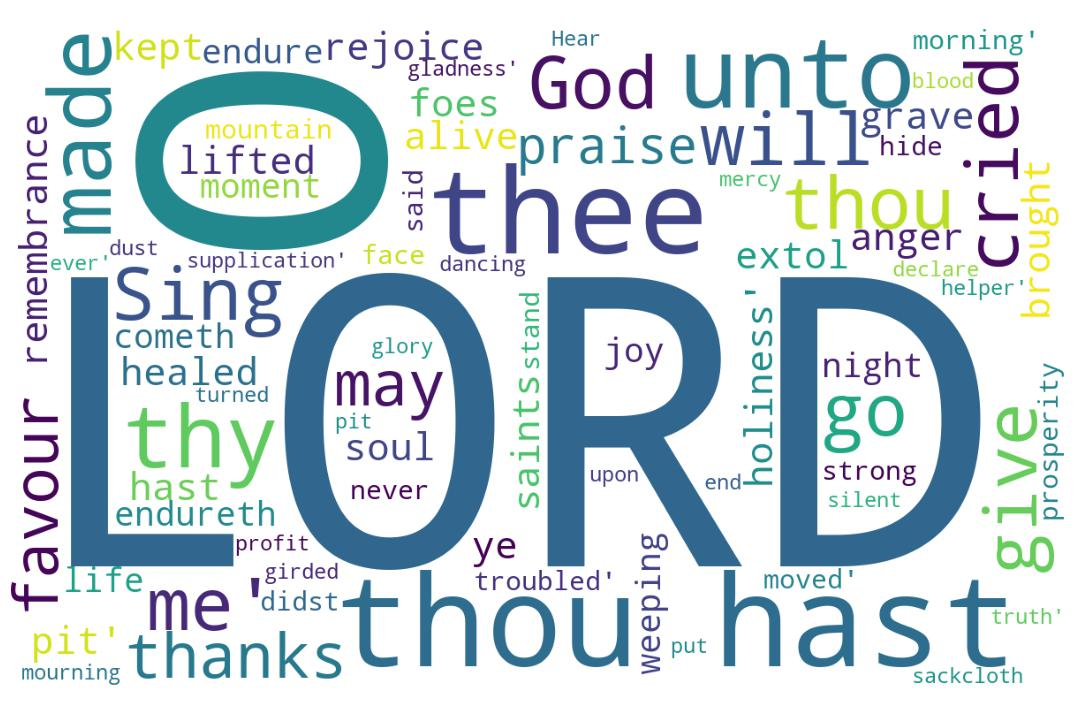
\includegraphics[width=\linewidth]{19OT-Psalms/Psalm30-WordCloud.jpg}
  \caption{Psalm 30 Word Cloud}
  \label{fig:Psalm 30 word Cloud}
\end{figure}
%%%%%%%%%%%%%%%%%%%%%%%%%%%%%%%%%%%%%%%%%
%%%%%%%%%%%%%%%%%%%%%%%%%%%%%%%%%%%%%%%%%

\marginpar{\scriptsize \centering \fcolorbox{bone}{lime}{\textbf{GOD'S FAVOUR}}\\ (Psalm 30:1--12) 
\begin{compactenum}[I.][8]
    \item David spared at the \textbf{Brink of Death} \index[scripture]{Psalms!Psa 030:03} (Psa 30:3)
    \item God's favor was David's \textbf{Basis for Deliverance} \index[scripture]{Psalms!Psa 030:05} (Psa 30:5)
    \item David's \textbf{Bad Declaration} \index[scripture]{Psalms!Psa 030:06} (Psa 30:6)
    \item David's \textbf{Better Decision}  \index[scripture]{Psalms!Psa 030:07} (Psa 30:7)
    \item David gets \textbf{Blessing instead of Dust} \index[scripture]{Psalms!Psa 030:09} (Psa 30:9)
    \item God changed David's \textbf{Bitterness into Dancing} \index[scripture]{Psalms!Psa 030:11} (Psa 30:11)
    \item David gets a \textbf{Bright Destiny} \index[scripture]{Psalms!Psa 030:12} (Psa 30:12)
\end{compactenum} }

\footnote{\textcolor[cmyk]{0.99998,1,0,0}{\hyperlink{TOC}{Return to end of Table of Contents.}}}\footnote{\href{https://www.audioverse.org/english/audiobibles/books/ENGKJV/O/Ps/1}{\textcolor[cmyk]{0.99998,1,0,0}{Psalms Audio}}}\textcolor[cmyk]{0.99998,1,0,0}{A Psalm \emph{and} Song \emph{at} the dedication of the house of David.}\\
\\
\textcolor[cmyk]{0.99998,1,0,0}{I will extol thee, O LORD; for thou hast lifted me up, and hast not made my foes to rejoice over me.}
[2] \textcolor[cmyk]{0.99998,1,0,0}{O LORD my God, I cried unto thee, and thou hast healed me.}
[3] \textcolor[cmyk]{0.99998,1,0,0}{O LORD, thou hast brought up my soul \fcolorbox{bone}{lime}{from the grave}: thou hast kept me alive, that I should not go down to the pit.}
[4] \textcolor[cmyk]{0.99998,1,0,0}{Sing unto the LORD, O ye saints of his, and give thanks at the remembrance of his holiness.}
[5] \textcolor[cmyk]{0.99998,1,0,0}{For his anger \emph{endureth} \emph{but} a moment; in \fcolorbox{bone}{lime}{his favour} \emph{is} life: weeping may endure for a night, but joy \emph{cometh} in the morning.}
[6] \textcolor[cmyk]{0.99998,1,0,0}{And in my prosperity I said, I shall \fcolorbox{bone}{lime}{never} be moved.}
[7] \textcolor[cmyk]{0.99998,1,0,0}{LORD, by \fcolorbox{bone}{lime}{thy favour} thou hast made my mountain to stand strong: thou didst hide thy face, \emph{and} I was troubled.}
[8] \textcolor[cmyk]{0.99998,1,0,0}{I \fcolorbox{bone}{lime}{cried to thee}, O LORD; and unto the LORD I made supplication.}
[9] \textcolor[cmyk]{0.99998,1,0,0}{What profit \emph{is} \emph{there} in my blood, when I go down to the pit? Shall the \fcolorbox{bone}{lime}{dust} praise thee? shall it declare thy truth?}
[10] \textcolor[cmyk]{0.99998,1,0,0}{Hear, O LORD, and have mercy upon me: LORD, be thou my helper.}
[11] \textcolor[cmyk]{0.99998,1,0,0}{Thou hast turned for me my mourning into \fcolorbox{bone}{lime}{dancing}: thou hast put off my sackcloth, and girded me with gladness;}
[12] \textcolor[cmyk]{0.99998,1,0,0}{To \fcolorbox{bone}{lime}{the end} that \emph{my} glory may sing praise to thee, and not be silent. O LORD my God, I will give thanks unto thee for ever.}
\section{Psalm 30 Comments}

\subsection{Numeric Nuggets}
There are 13 words in Psalm 30:2, Psalm 30:8, and Psalm 30:10.
%\input{19OT-Psalms/Psalm30-WordIndex}
\section{Psalm 30 Outlines}

\subsection{My Outlines}

\subsubsection{God's Favour}
\index[speaker]{Keith Anthony!Psalm 030 (God's Favour)}
\index[series]{Psalms (Keith Anthony)!Psalm 030 (God's Favour)}
\index[date]{2014/11/02!Psalm 030 (God's Favour) (Keith Anthony)}
Introduction: The superscription for Psalm 30 reads ``A Psalm and Song at the dedication of the house of David,'' connecting it with the dedication of the site for the Temple (\index[scripture]{1 Chronicles!1Chr 21:26}1 Chronicles 21:26 and \index[scripture]{1 Chronicles!1Chr 22: 1}1 Chronicles 22:1). The psalm has three verses (\index[scripture]{Psalms!Psa 030:02}Psalm 30:2, \index[scripture]{Psalms!Psa 030:08}Psalm 30:8, and \index[scripture]{Psalms!Psa 030:10}Psalm 30:10) with 13 words, showing that despite David's sin and deep-down rebellion, God still kept His covenant with David. Instances of the number 13 typically indicate rebellion, or an opportunity to choose between rebellion or obedience, or here, repentance. Psalm 30:3 indicates that God had delivered David, at some point, from the brink of death. Some hold that Psalm 30:6-7 refers to the plague God sent in response to David's census, done against God's command (see 2 Samuel 24 and 1 Chronicles 21). Consider aspects of God's favor upon David:
\begin{compactenum}
    \item David was spared at the \textbf{Brink of Death} \index[scripture]{Psalms!Psa 030:03} (Psa 30:3)
    \item God's favor was David's \textbf{Basis for Deliverance} \index[scripture]{Psalms!Psa 030:05} (Psa 30:5)
    \item God's favor was given despite David's \textbf{Bad Declaration} - David was comfortable and secure and apparently forgot the source of all his blessings. \index[scripture]{Psalms!Psa 030:06} (Psa 30:6)
    \item God's seeming absence results in David's \textbf{Better Decision}  \index[scripture]{Psalms!Psa 030:07} (Psa 30:7)
    \item Because of God's favor David gets \textbf{Blessing instead of Dust} \index[scripture]{Psalms!Psa 030:09} (Psa 30:9)
    \item God changed David's \textbf{Bitterness into Dancing} \index[scripture]{Psalms!Psa 030:11} (Psa 30:11)
    \item Because of God's Favor, David has a \textbf{Bright Destiny} \index[scripture]{Psalms!Psa 030:12} (Psa 30:12)\\
\end{compactenum}
Do you have God's favor in your life? Do you even want it?

% made 3 (1, 7, 8)  may 2 (5, 12)  me 7 (1 (2x), 2, 3, 10, 11 (2x)) mercy 1 (10) moment 1 (5) morning 1(5) mountain 1 (7)  mourning 1 (11) moved 1 (6) my 10 (1, 2, 3, 6, 7, 9, 10, 11 (2x), 12) 
\subsection{Outlines from Others}

%\input{19OT-Psalms/Psalm30Statistics}
\subsection{Psalm 30 Repeated Phrases}


%%%%%%%%%%
%%%%%%%%%%
\normalsize
 
\begin{center}
\begin{longtable}{|p{3.0in}|p{0.5in}|}
\caption[Psalm 30 Repeated Phrases]{Psalm 30 Repeated Phrases}\label{table:Repeated Phrases Psalm 30} \\
\hline \multicolumn{1}{|c|}{\textbf{Phrase}} & \multicolumn{1}{c|}{\textbf{Frequency}} \\ \hline 
\endfirsthead
 
\multicolumn{2}{c}
{{\bfseries \tablename\ \thetable{} -- continued from previous page}} \\  
\hline \multicolumn{1}{|c|}{\textbf{Phrase}} & \multicolumn{1}{c|}{\textbf{Frequency}} \\ \hline 
\endhead
 
\hline \multicolumn{2}{c}{{ }} \\ \hline
\endfoot 
O LORD & 6\\ \hline 
thou hast & 6\\ \hline 
\end{longtable}
\end{center}



%%%%%%%%%%
%%%%%%%%%%




\chapter{Psalm 31}

\begin{figure}
  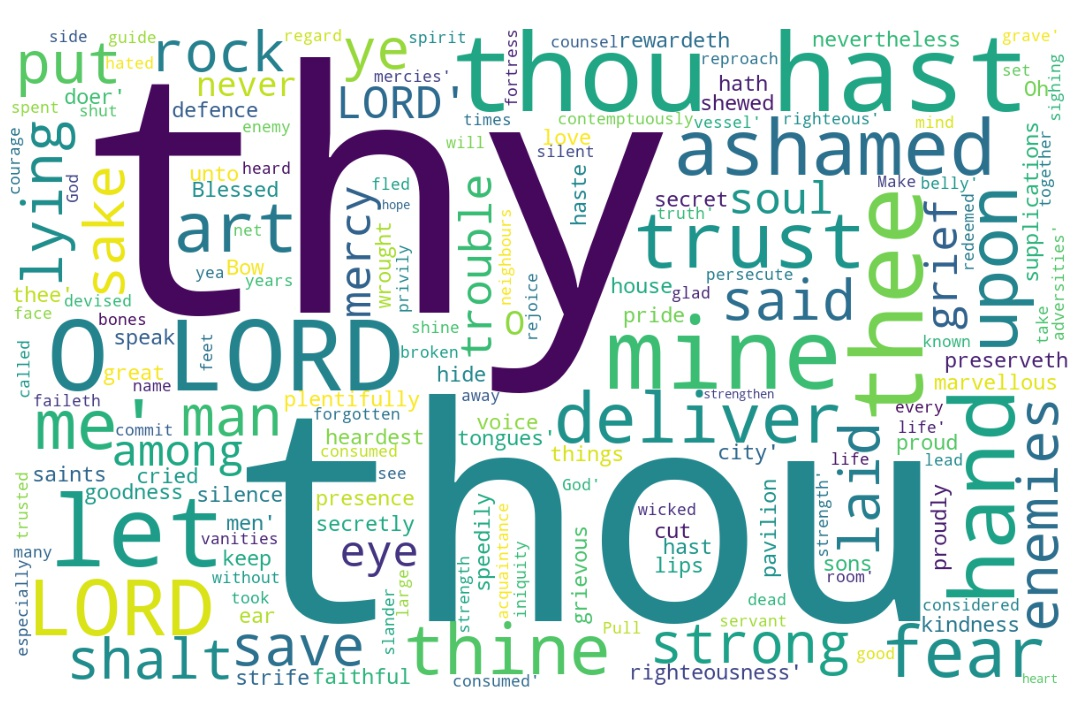
\includegraphics[width=\linewidth]{19OT-Psalms/Psalm31-WordCloud.jpg}
  \caption{Psalm 31 Word Cloud}
  \label{fig:Psalm 31 word Cloud}
\end{figure}


\marginpar{\scriptsize \centering \fcolorbox{bone}{lime}{\textbf{DAVID'S CRY}}\\ (Psalm 31:1--24) 
\begin{compactenum}[I.][8]
    \item \textbf{Special Trust} \index[scripture]{Psalms!Psa 031:01}(Psa 31:1)  
    \item \textbf{Secret Traps} \index[scripture]{Psalms!Psa 031:04}(Psa 31:4)  
    \item \textbf{Singular Trouble} \index[scripture]{Psalms!Psa 031:07}(Psa 31:7)  
    \item \textbf{Slandered Times} \index[scripture]{Psalms!Psa 031:13}(Psa 31:13)  
    \item \textbf{Sovereign Troops} \index[scripture]{Psalms!Psa 031:15}(Psa 31:15)  
    \item \textbf{Striving Tongues} \index[scripture]{Psalms!Psa 031:20}(Psa 31:20)  
    \item \textbf{Silenced Troublemaker} \index[scripture]{Psalms!Psa 031:23}(Psa 31:23)  
\end{compactenum} }

\footnote{\textcolor[cmyk]{0.99998,1,0,0}{\hyperlink{TOC}{Return to end of Table of Contents.}}}\footnote{\href{https://audiobible.com/bible}{\textcolor[cmyk]{0.99998,1,0,0}{Psalms Audio}}}\textcolor[cmyk]{0.99998,1,0,0}{To the chief Musician, A Psalm of David.}\\
\\
\textcolor[cmyk]{0.99998,1,0,0}{In thee, O LORD, do I put my \fcolorbox{bone}{lime}{trust}; let me never be ashamed: deliver me in thy righteousness.}
[2] \textcolor[cmyk]{0.99998,1,0,0}{Bow down thine ear to me; deliver me speedily: be thou my strong rock, for an house of defence to save me.}
[3] \textcolor[cmyk]{0.99998,1,0,0}{For thou \emph{art} my rock and my fortress; therefore for thy name's sake lead me, and guide me.}
[4] \textcolor[cmyk]{0.99998,1,0,0}{Pull me out of \fcolorbox{bone}{lime}{the net} that they have laid privily for me: for thou \emph{art} my strength.}\footnote{\textbf{Psalm 9:15} - The heathen are sunk down in the pit that they made: in the net which they hid is their own foot taken.}\footnote{\textbf{Psalm 25:15} - Mine eyes are ever toward the LORD; for he shall pluck my feet out of the net.}\footnote{\textbf{Psalm 66:11} - Thou broughtest us into the net; thou laidst affliction upon our loins.}\footnote{\textbf{Proverb 1:17} - Surely in vain the net is spread in the sight of any bird.}\footnote{\textbf{Proverb 12:12} - The wicked desireth the net of evil men: but the root of the righteous yieldeth fruit.}
[5] \textcolor[cmyk]{0.99998,1,0,0}{Into thine hand I commit my spirit: thou hast redeemed me, O LORD God of truth.}
[6] \textcolor[cmyk]{0.99998,1,0,0}{I have hated them that regard lying vanities: but I trust in the LORD.}
[7] \textcolor[cmyk]{0.99998,1,0,0}{I will be glad and rejoice in thy mercy: for thou hast considered my \fcolorbox{bone}{lime}{trouble}; thou hast known my soul in adversities;}
[8] \textcolor[cmyk]{0.99998,1,0,0}{And hast not shut me up into the hand of the enemy: thou hast set my feet in a large room.}
[9] \textcolor[cmyk]{0.99998,1,0,0}{Have mercy upon me, O LORD, for I am in trouble: mine eye is consumed with grief, \emph{yea}, my soul and my belly.}
[10] \textcolor[cmyk]{0.99998,1,0,0}{For my life is spent with grief, and my years with sighing: my strength faileth because of mine iniquity, and my bones are consumed.}
[11] \textcolor[cmyk]{0.99998,1,0,0}{I was a reproach among all mine enemies, but especially among my neighbours, and a fear to mine acquaintance: they that did see me without fled from me.}
[12] \textcolor[cmyk]{0.99998,1,0,0}{I am forgotten as a dead man out of mind: I am like a broken vessel.}
[13] \textcolor[cmyk]{0.99998,1,0,0}{For I have heard the \fcolorbox{bone}{lime}{slander} of many: fear \emph{was} on every side: while they took counsel together against me, they devised to take away my life.}
[14] \textcolor[cmyk]{0.99998,1,0,0}{But I trusted in thee, O LORD: I said, Thou \emph{art} my God.}
[15] \textcolor[cmyk]{0.99998,1,0,0}{My times \emph{are} in thy hand: deliver me from the hand of mine \fcolorbox{bone}{lime}{enemies}, and from them that persecute me.}
[16] \textcolor[cmyk]{0.99998,1,0,0}{Make thy face to shine upon thy servant: save me for thy mercies' sake.}
[17] \textcolor[cmyk]{0.99998,1,0,0}{Let me not be ashamed, O LORD; for I have called upon thee: let the wicked be ashamed, \emph{and} let them be silent in the grave.}
[18] \textcolor[cmyk]{0.99998,1,0,0}{Let the lying lips be put to silence; which speak grievous things proudly and contemptuously against the righteous.}
[19] \textcolor[cmyk]{0.99998,1,0,0}{\emph{Oh} how great \emph{is} thy goodness, which thou hast laid up for them that fear thee; \emph{which} thou hast wrought for them that trust in thee before the sons of men!}
[20] \textcolor[cmyk]{0.99998,1,0,0}{Thou shalt hide them in the secret of thy presence from the pride of man: thou shalt keep them secretly in a pavilion from the strife of \fcolorbox{bone}{lime}{tongues}.}
[21] \textcolor[cmyk]{0.99998,1,0,0}{Blessed \emph{be} the LORD: for he hath shewed me his marvellous kindness in a strong city.}
[22] \textcolor[cmyk]{0.99998,1,0,0}{For I said in my haste, I am cut off from before thine eyes: nevertheless thou heardest the voice of my supplications when I cried unto thee.}
[23] \textcolor[cmyk]{0.99998,1,0,0}{O love the LORD, all ye his saints: \emph{for} the LORD preserveth the faithful, and plentifully rewardeth the \fcolorbox{bone}{lime}{proud doer}.}
[24] \textcolor[cmyk]{0.99998,1,0,0}{Be of good courage, and he shall strengthen your heart, all ye that hope in the LORD.}
\section{Psalm 31 Comments}

\subsection{Numeric Nuggets}
The 13-letter words ``righteousness'' and ``supplications'' are found in the chapter. Psalm 31:14 has 13 words.

\subsection{Psalm 31:4}
The phrase ``the net'' is found 13 times in scripture. %, 6 of those times in a negative sense, as a trap set by evil men for God's people.  In Exodus, the ``net'' was part of the altar.  In the gospels, the ``net'' was cast into the sea to capture fish, with the fish representing redeemed souls.
%\index[NWIV]{19!Psalms!Psa 31:1}\index[AWIP]{In!Psalms!Psa 31:1}\index[AWIP]{thee!Psalms!Psa 31:1}\index[AWIP]{O!Psalms!Psa 31:1}\index[AWIP]{LORD!Psalms!Psa 31:1}\index[AWIP]{do!Psalms!Psa 31:1}\index[AWIP]{I!Psalms!Psa 31:1}\index[AWIP]{put!Psalms!Psa 31:1}\index[AWIP]{my!Psalms!Psa 31:1}\index[AWIP]{trust!Psalms!Psa 31:1}\index[AWIP]{let!Psalms!Psa 31:1}\index[AWIP]{me!Psalms!Psa 31:1}\index[AWIP]{me!Psalms!Psa 31:1 (2)}\index[AWIP]{never!Psalms!Psa 31:1}\index[AWIP]{be!Psalms!Psa 31:1}\index[AWIP]{ashamed!Psalms!Psa 31:1}\index[AWIP]{deliver!Psalms!Psa 31:1}\index[AWIP]{in!Psalms!Psa 31:1}\index[AWIP]{thy!Psalms!Psa 31:1}\index[AWIP]{righteousness!Psalms!Psa 31:1}

\index[NWIV]{22!Psalms!Psa 31:2}\index[AWIP]{Bow!Psalms!Psa 31:2}\index[AWIP]{down!Psalms!Psa 31:2}\index[AWIP]{thine!Psalms!Psa 31:2}\index[AWIP]{ear!Psalms!Psa 31:2}\index[AWIP]{to!Psalms!Psa 31:2}\index[AWIP]{to!Psalms!Psa 31:2 (2)}\index[AWIP]{me!Psalms!Psa 31:2}\index[AWIP]{me!Psalms!Psa 31:2 (2)}\index[AWIP]{me!Psalms!Psa 31:2 (3)}\index[AWIP]{deliver!Psalms!Psa 31:2}\index[AWIP]{speedily!Psalms!Psa 31:2}\index[AWIP]{be!Psalms!Psa 31:2}\index[AWIP]{thou!Psalms!Psa 31:2}\index[AWIP]{my!Psalms!Psa 31:2}\index[AWIP]{strong!Psalms!Psa 31:2}\index[AWIP]{rock!Psalms!Psa 31:2}\index[AWIP]{for!Psalms!Psa 31:2}\index[AWIP]{an!Psalms!Psa 31:2}\index[AWIP]{house!Psalms!Psa 31:2}\index[AWIP]{of!Psalms!Psa 31:2}\index[AWIP]{defence!Psalms!Psa 31:2}\index[AWIP]{save!Psalms!Psa 31:2}

\index[NWIV]{18!Psalms!Psa 31:3}\index[AWIP]{For!Psalms!Psa 31:3}\index[AWIP]{thou!Psalms!Psa 31:3}\index[AWIP]{\emph{art}!Psalms!Psa 31:3}\index[AWIP]{my!Psalms!Psa 31:3}\index[AWIP]{my!Psalms!Psa 31:3 (2)}\index[AWIP]{rock!Psalms!Psa 31:3}\index[AWIP]{and!Psalms!Psa 31:3}\index[AWIP]{and!Psalms!Psa 31:3 (2)}\index[AWIP]{fortress!Psalms!Psa 31:3}\index[AWIP]{therefore!Psalms!Psa 31:3}\index[AWIP]{for!Psalms!Psa 31:3}\index[AWIP]{thy!Psalms!Psa 31:3}\index[AWIP]{name's!Psalms!Psa 31:3}\index[AWIP]{sake!Psalms!Psa 31:3}\index[AWIP]{lead!Psalms!Psa 31:3}\index[AWIP]{me!Psalms!Psa 31:3}\index[AWIP]{me!Psalms!Psa 31:3 (2)}\index[AWIP]{guide!Psalms!Psa 31:3}\index[AWIP]{\emph{art}!Psalms!Psa 31:3}

\index[NWIV]{18!Psalms!Psa 31:4}\index[AWIP]{Pull!Psalms!Psa 31:4}\index[AWIP]{me!Psalms!Psa 31:4}\index[AWIP]{me!Psalms!Psa 31:4 (2)}\index[AWIP]{out!Psalms!Psa 31:4}\index[AWIP]{of!Psalms!Psa 31:4}\index[AWIP]{the!Psalms!Psa 31:4}\index[AWIP]{net!Psalms!Psa 31:4}\index[AWIP]{that!Psalms!Psa 31:4}\index[AWIP]{they!Psalms!Psa 31:4}\index[AWIP]{have!Psalms!Psa 31:4}\index[AWIP]{laid!Psalms!Psa 31:4}\index[AWIP]{privily!Psalms!Psa 31:4}\index[AWIP]{for!Psalms!Psa 31:4}\index[AWIP]{for!Psalms!Psa 31:4 (2)}\index[AWIP]{thou!Psalms!Psa 31:4}\index[AWIP]{\emph{art}!Psalms!Psa 31:4}\index[AWIP]{my!Psalms!Psa 31:4}\index[AWIP]{strength!Psalms!Psa 31:4}\index[AWIP]{\emph{art}!Psalms!Psa 31:4}

\index[NWIV]{16!Psalms!Psa 31:5}\index[AWIP]{Into!Psalms!Psa 31:5}\index[AWIP]{thine!Psalms!Psa 31:5}\index[AWIP]{hand!Psalms!Psa 31:5}\index[AWIP]{I!Psalms!Psa 31:5}\index[AWIP]{commit!Psalms!Psa 31:5}\index[AWIP]{my!Psalms!Psa 31:5}\index[AWIP]{spirit!Psalms!Psa 31:5}\index[AWIP]{thou!Psalms!Psa 31:5}\index[AWIP]{hast!Psalms!Psa 31:5}\index[AWIP]{redeemed!Psalms!Psa 31:5}\index[AWIP]{me!Psalms!Psa 31:5}\index[AWIP]{O!Psalms!Psa 31:5}\index[AWIP]{LORD!Psalms!Psa 31:5}\index[AWIP]{God!Psalms!Psa 31:5}\index[AWIP]{of!Psalms!Psa 31:5}\index[AWIP]{truth!Psalms!Psa 31:5}

\index[NWIV]{14!Psalms!Psa 31:6}\index[AWIP]{I!Psalms!Psa 31:6}\index[AWIP]{I!Psalms!Psa 31:6 (2)}\index[AWIP]{have!Psalms!Psa 31:6}\index[AWIP]{hated!Psalms!Psa 31:6}\index[AWIP]{them!Psalms!Psa 31:6}\index[AWIP]{that!Psalms!Psa 31:6}\index[AWIP]{regard!Psalms!Psa 31:6}\index[AWIP]{lying!Psalms!Psa 31:6}\index[AWIP]{vanities!Psalms!Psa 31:6}\index[AWIP]{but!Psalms!Psa 31:6}\index[AWIP]{trust!Psalms!Psa 31:6}\index[AWIP]{in!Psalms!Psa 31:6}\index[AWIP]{the!Psalms!Psa 31:6}\index[AWIP]{LORD!Psalms!Psa 31:6}

\index[NWIV]{22!Psalms!Psa 31:7}\index[AWIP]{I!Psalms!Psa 31:7}\index[AWIP]{will!Psalms!Psa 31:7}\index[AWIP]{be!Psalms!Psa 31:7}\index[AWIP]{glad!Psalms!Psa 31:7}\index[AWIP]{and!Psalms!Psa 31:7}\index[AWIP]{rejoice!Psalms!Psa 31:7}\index[AWIP]{in!Psalms!Psa 31:7}\index[AWIP]{in!Psalms!Psa 31:7 (2)}\index[AWIP]{thy!Psalms!Psa 31:7}\index[AWIP]{mercy!Psalms!Psa 31:7}\index[AWIP]{for!Psalms!Psa 31:7}\index[AWIP]{thou!Psalms!Psa 31:7}\index[AWIP]{thou!Psalms!Psa 31:7 (2)}\index[AWIP]{hast!Psalms!Psa 31:7}\index[AWIP]{hast!Psalms!Psa 31:7 (2)}\index[AWIP]{considered!Psalms!Psa 31:7}\index[AWIP]{my!Psalms!Psa 31:7}\index[AWIP]{my!Psalms!Psa 31:7 (2)}\index[AWIP]{trouble!Psalms!Psa 31:7}\index[AWIP]{known!Psalms!Psa 31:7}\index[AWIP]{soul!Psalms!Psa 31:7}\index[AWIP]{adversities!Psalms!Psa 31:7}

\index[NWIV]{21!Psalms!Psa 31:8}\index[AWIP]{And!Psalms!Psa 31:8}\index[AWIP]{hast!Psalms!Psa 31:8}\index[AWIP]{hast!Psalms!Psa 31:8 (2)}\index[AWIP]{not!Psalms!Psa 31:8}\index[AWIP]{shut!Psalms!Psa 31:8}\index[AWIP]{me!Psalms!Psa 31:8}\index[AWIP]{up!Psalms!Psa 31:8}\index[AWIP]{into!Psalms!Psa 31:8}\index[AWIP]{the!Psalms!Psa 31:8}\index[AWIP]{the!Psalms!Psa 31:8 (2)}\index[AWIP]{hand!Psalms!Psa 31:8}\index[AWIP]{of!Psalms!Psa 31:8}\index[AWIP]{enemy!Psalms!Psa 31:8}\index[AWIP]{thou!Psalms!Psa 31:8}\index[AWIP]{set!Psalms!Psa 31:8}\index[AWIP]{my!Psalms!Psa 31:8}\index[AWIP]{feet!Psalms!Psa 31:8}\index[AWIP]{in!Psalms!Psa 31:8}\index[AWIP]{a!Psalms!Psa 31:8}\index[AWIP]{large!Psalms!Psa 31:8}\index[AWIP]{room!Psalms!Psa 31:8}

\index[NWIV]{23!Psalms!Psa 31:9}\index[AWIP]{Have!Psalms!Psa 31:9}\index[AWIP]{mercy!Psalms!Psa 31:9}\index[AWIP]{upon!Psalms!Psa 31:9}\index[AWIP]{me!Psalms!Psa 31:9}\index[AWIP]{O!Psalms!Psa 31:9}\index[AWIP]{LORD!Psalms!Psa 31:9}\index[AWIP]{for!Psalms!Psa 31:9}\index[AWIP]{I!Psalms!Psa 31:9}\index[AWIP]{am!Psalms!Psa 31:9}\index[AWIP]{in!Psalms!Psa 31:9}\index[AWIP]{trouble!Psalms!Psa 31:9}\index[AWIP]{mine!Psalms!Psa 31:9}\index[AWIP]{eye!Psalms!Psa 31:9}\index[AWIP]{is!Psalms!Psa 31:9}\index[AWIP]{consumed!Psalms!Psa 31:9}\index[AWIP]{with!Psalms!Psa 31:9}\index[AWIP]{grief!Psalms!Psa 31:9}\index[AWIP]{\emph{yea}!Psalms!Psa 31:9}\index[AWIP]{my!Psalms!Psa 31:9}\index[AWIP]{my!Psalms!Psa 31:9 (2)}\index[AWIP]{soul!Psalms!Psa 31:9}\index[AWIP]{and!Psalms!Psa 31:9}\index[AWIP]{belly!Psalms!Psa 31:9}\index[AWIP]{\emph{yea}!Psalms!Psa 31:9}

\index[NWIV]{24!Psalms!Psa 31:10}\index[AWIP]{For!Psalms!Psa 31:10}\index[AWIP]{my!Psalms!Psa 31:10}\index[AWIP]{my!Psalms!Psa 31:10 (2)}\index[AWIP]{my!Psalms!Psa 31:10 (3)}\index[AWIP]{my!Psalms!Psa 31:10 (4)}\index[AWIP]{life!Psalms!Psa 31:10}\index[AWIP]{is!Psalms!Psa 31:10}\index[AWIP]{spent!Psalms!Psa 31:10}\index[AWIP]{with!Psalms!Psa 31:10}\index[AWIP]{with!Psalms!Psa 31:10 (2)}\index[AWIP]{grief!Psalms!Psa 31:10}\index[AWIP]{and!Psalms!Psa 31:10}\index[AWIP]{and!Psalms!Psa 31:10 (2)}\index[AWIP]{years!Psalms!Psa 31:10}\index[AWIP]{sighing!Psalms!Psa 31:10}\index[AWIP]{strength!Psalms!Psa 31:10}\index[AWIP]{faileth!Psalms!Psa 31:10}\index[AWIP]{because!Psalms!Psa 31:10}\index[AWIP]{of!Psalms!Psa 31:10}\index[AWIP]{mine!Psalms!Psa 31:10}\index[AWIP]{iniquity!Psalms!Psa 31:10}\index[AWIP]{bones!Psalms!Psa 31:10}\index[AWIP]{are!Psalms!Psa 31:10}\index[AWIP]{consumed!Psalms!Psa 31:10}

\index[NWIV]{28!Psalms!Psa 31:11}\index[AWIP]{I!Psalms!Psa 31:11}\index[AWIP]{was!Psalms!Psa 31:11}\index[AWIP]{a!Psalms!Psa 31:11}\index[AWIP]{a!Psalms!Psa 31:11 (2)}\index[AWIP]{reproach!Psalms!Psa 31:11}\index[AWIP]{among!Psalms!Psa 31:11}\index[AWIP]{among!Psalms!Psa 31:11 (2)}\index[AWIP]{all!Psalms!Psa 31:11}\index[AWIP]{mine!Psalms!Psa 31:11}\index[AWIP]{mine!Psalms!Psa 31:11 (2)}\index[AWIP]{enemies!Psalms!Psa 31:11}\index[AWIP]{but!Psalms!Psa 31:11}\index[AWIP]{especially!Psalms!Psa 31:11}\index[AWIP]{my!Psalms!Psa 31:11}\index[AWIP]{neighbours!Psalms!Psa 31:11}\index[AWIP]{and!Psalms!Psa 31:11}\index[AWIP]{fear!Psalms!Psa 31:11}\index[AWIP]{to!Psalms!Psa 31:11}\index[AWIP]{acquaintance!Psalms!Psa 31:11}\index[AWIP]{they!Psalms!Psa 31:11}\index[AWIP]{that!Psalms!Psa 31:11}\index[AWIP]{did!Psalms!Psa 31:11}\index[AWIP]{see!Psalms!Psa 31:11}\index[AWIP]{me!Psalms!Psa 31:11}\index[AWIP]{me!Psalms!Psa 31:11 (2)}\index[AWIP]{without!Psalms!Psa 31:11}\index[AWIP]{fled!Psalms!Psa 31:11}\index[AWIP]{from!Psalms!Psa 31:11}

\index[NWIV]{16!Psalms!Psa 31:12}\index[AWIP]{I!Psalms!Psa 31:12}\index[AWIP]{I!Psalms!Psa 31:12 (2)}\index[AWIP]{am!Psalms!Psa 31:12}\index[AWIP]{am!Psalms!Psa 31:12 (2)}\index[AWIP]{forgotten!Psalms!Psa 31:12}\index[AWIP]{as!Psalms!Psa 31:12}\index[AWIP]{a!Psalms!Psa 31:12}\index[AWIP]{a!Psalms!Psa 31:12 (2)}\index[AWIP]{dead!Psalms!Psa 31:12}\index[AWIP]{man!Psalms!Psa 31:12}\index[AWIP]{out!Psalms!Psa 31:12}\index[AWIP]{of!Psalms!Psa 31:12}\index[AWIP]{mind!Psalms!Psa 31:12}\index[AWIP]{like!Psalms!Psa 31:12}\index[AWIP]{broken!Psalms!Psa 31:12}\index[AWIP]{vessel!Psalms!Psa 31:12}

\index[NWIV]{27!Psalms!Psa 31:13}\index[AWIP]{For!Psalms!Psa 31:13}\index[AWIP]{I!Psalms!Psa 31:13}\index[AWIP]{have!Psalms!Psa 31:13}\index[AWIP]{heard!Psalms!Psa 31:13}\index[AWIP]{the!Psalms!Psa 31:13}\index[AWIP]{slander!Psalms!Psa 31:13}\index[AWIP]{of!Psalms!Psa 31:13}\index[AWIP]{many!Psalms!Psa 31:13}\index[AWIP]{fear!Psalms!Psa 31:13}\index[AWIP]{\emph{was}!Psalms!Psa 31:13}\index[AWIP]{on!Psalms!Psa 31:13}\index[AWIP]{every!Psalms!Psa 31:13}\index[AWIP]{side!Psalms!Psa 31:13}\index[AWIP]{while!Psalms!Psa 31:13}\index[AWIP]{they!Psalms!Psa 31:13}\index[AWIP]{they!Psalms!Psa 31:13 (2)}\index[AWIP]{took!Psalms!Psa 31:13}\index[AWIP]{counsel!Psalms!Psa 31:13}\index[AWIP]{together!Psalms!Psa 31:13}\index[AWIP]{against!Psalms!Psa 31:13}\index[AWIP]{me!Psalms!Psa 31:13}\index[AWIP]{devised!Psalms!Psa 31:13}\index[AWIP]{to!Psalms!Psa 31:13}\index[AWIP]{take!Psalms!Psa 31:13}\index[AWIP]{away!Psalms!Psa 31:13}\index[AWIP]{my!Psalms!Psa 31:13}\index[AWIP]{life!Psalms!Psa 31:13}\index[AWIP]{\emph{was}!Psalms!Psa 31:13}

\index[NWIV]{13!Psalms!Psa 31:14}\index[AWIP]{But!Psalms!Psa 31:14}\index[AWIP]{I!Psalms!Psa 31:14}\index[AWIP]{I!Psalms!Psa 31:14 (2)}\index[AWIP]{trusted!Psalms!Psa 31:14}\index[AWIP]{in!Psalms!Psa 31:14}\index[AWIP]{thee!Psalms!Psa 31:14}\index[AWIP]{O!Psalms!Psa 31:14}\index[AWIP]{LORD!Psalms!Psa 31:14}\index[AWIP]{said!Psalms!Psa 31:14}\index[AWIP]{Thou!Psalms!Psa 31:14}\index[AWIP]{\emph{art}!Psalms!Psa 31:14}\index[AWIP]{my!Psalms!Psa 31:14}\index[AWIP]{God!Psalms!Psa 31:14}\index[AWIP]{\emph{art}!Psalms!Psa 31:14}

\index[NWIV]{20!Psalms!Psa 31:15}\index[AWIP]{My!Psalms!Psa 31:15}\index[AWIP]{times!Psalms!Psa 31:15}\index[AWIP]{\emph{are}!Psalms!Psa 31:15}\index[AWIP]{in!Psalms!Psa 31:15}\index[AWIP]{thy!Psalms!Psa 31:15}\index[AWIP]{hand!Psalms!Psa 31:15}\index[AWIP]{hand!Psalms!Psa 31:15 (2)}\index[AWIP]{deliver!Psalms!Psa 31:15}\index[AWIP]{me!Psalms!Psa 31:15}\index[AWIP]{me!Psalms!Psa 31:15 (2)}\index[AWIP]{from!Psalms!Psa 31:15}\index[AWIP]{from!Psalms!Psa 31:15 (2)}\index[AWIP]{the!Psalms!Psa 31:15}\index[AWIP]{of!Psalms!Psa 31:15}\index[AWIP]{mine!Psalms!Psa 31:15}\index[AWIP]{enemies!Psalms!Psa 31:15}\index[AWIP]{and!Psalms!Psa 31:15}\index[AWIP]{them!Psalms!Psa 31:15}\index[AWIP]{that!Psalms!Psa 31:15}\index[AWIP]{persecute!Psalms!Psa 31:15}\index[AWIP]{\emph{are}!Psalms!Psa 31:15}

\index[NWIV]{14!Psalms!Psa 31:16}\index[AWIP]{Make!Psalms!Psa 31:16}\index[AWIP]{thy!Psalms!Psa 31:16}\index[AWIP]{thy!Psalms!Psa 31:16 (2)}\index[AWIP]{thy!Psalms!Psa 31:16 (3)}\index[AWIP]{face!Psalms!Psa 31:16}\index[AWIP]{to!Psalms!Psa 31:16}\index[AWIP]{shine!Psalms!Psa 31:16}\index[AWIP]{upon!Psalms!Psa 31:16}\index[AWIP]{servant!Psalms!Psa 31:16}\index[AWIP]{save!Psalms!Psa 31:16}\index[AWIP]{me!Psalms!Psa 31:16}\index[AWIP]{for!Psalms!Psa 31:16}\index[AWIP]{mercies'!Psalms!Psa 31:16}\index[AWIP]{sake!Psalms!Psa 31:16}

\index[NWIV]{26!Psalms!Psa 31:17}\index[AWIP]{Let!Psalms!Psa 31:17}\index[AWIP]{me!Psalms!Psa 31:17}\index[AWIP]{not!Psalms!Psa 31:17}\index[AWIP]{be!Psalms!Psa 31:17}\index[AWIP]{be!Psalms!Psa 31:17 (2)}\index[AWIP]{be!Psalms!Psa 31:17 (3)}\index[AWIP]{ashamed!Psalms!Psa 31:17}\index[AWIP]{ashamed!Psalms!Psa 31:17 (2)}\index[AWIP]{O!Psalms!Psa 31:17}\index[AWIP]{LORD!Psalms!Psa 31:17}\index[AWIP]{for!Psalms!Psa 31:17}\index[AWIP]{I!Psalms!Psa 31:17}\index[AWIP]{have!Psalms!Psa 31:17}\index[AWIP]{called!Psalms!Psa 31:17}\index[AWIP]{upon!Psalms!Psa 31:17}\index[AWIP]{thee!Psalms!Psa 31:17}\index[AWIP]{let!Psalms!Psa 31:17}\index[AWIP]{let!Psalms!Psa 31:17 (2)}\index[AWIP]{the!Psalms!Psa 31:17}\index[AWIP]{the!Psalms!Psa 31:17 (2)}\index[AWIP]{wicked!Psalms!Psa 31:17}\index[AWIP]{\emph{and}!Psalms!Psa 31:17}\index[AWIP]{them!Psalms!Psa 31:17}\index[AWIP]{silent!Psalms!Psa 31:17}\index[AWIP]{in!Psalms!Psa 31:17}\index[AWIP]{grave!Psalms!Psa 31:17}\index[AWIP]{\emph{and}!Psalms!Psa 31:17}

\index[NWIV]{18!Psalms!Psa 31:18}\index[AWIP]{Let!Psalms!Psa 31:18}\index[AWIP]{the!Psalms!Psa 31:18}\index[AWIP]{the!Psalms!Psa 31:18 (2)}\index[AWIP]{lying!Psalms!Psa 31:18}\index[AWIP]{lips!Psalms!Psa 31:18}\index[AWIP]{be!Psalms!Psa 31:18}\index[AWIP]{put!Psalms!Psa 31:18}\index[AWIP]{to!Psalms!Psa 31:18}\index[AWIP]{silence!Psalms!Psa 31:18}\index[AWIP]{which!Psalms!Psa 31:18}\index[AWIP]{speak!Psalms!Psa 31:18}\index[AWIP]{grievous!Psalms!Psa 31:18}\index[AWIP]{things!Psalms!Psa 31:18}\index[AWIP]{proudly!Psalms!Psa 31:18}\index[AWIP]{and!Psalms!Psa 31:18}\index[AWIP]{contemptuously!Psalms!Psa 31:18}\index[AWIP]{against!Psalms!Psa 31:18}\index[AWIP]{righteous!Psalms!Psa 31:18}

\index[NWIV]{31!Psalms!Psa 31:19}\index[AWIP]{\emph{Oh}!Psalms!Psa 31:19}\index[AWIP]{how!Psalms!Psa 31:19}\index[AWIP]{great!Psalms!Psa 31:19}\index[AWIP]{\emph{is}!Psalms!Psa 31:19}\index[AWIP]{thy!Psalms!Psa 31:19}\index[AWIP]{goodness!Psalms!Psa 31:19}\index[AWIP]{which!Psalms!Psa 31:19}\index[AWIP]{thou!Psalms!Psa 31:19}\index[AWIP]{thou!Psalms!Psa 31:19 (2)}\index[AWIP]{hast!Psalms!Psa 31:19}\index[AWIP]{hast!Psalms!Psa 31:19 (2)}\index[AWIP]{laid!Psalms!Psa 31:19}\index[AWIP]{up!Psalms!Psa 31:19}\index[AWIP]{for!Psalms!Psa 31:19}\index[AWIP]{for!Psalms!Psa 31:19 (2)}\index[AWIP]{them!Psalms!Psa 31:19}\index[AWIP]{them!Psalms!Psa 31:19 (2)}\index[AWIP]{that!Psalms!Psa 31:19}\index[AWIP]{that!Psalms!Psa 31:19 (2)}\index[AWIP]{fear!Psalms!Psa 31:19}\index[AWIP]{thee!Psalms!Psa 31:19}\index[AWIP]{thee!Psalms!Psa 31:19 (2)}\index[AWIP]{\emph{which}!Psalms!Psa 31:19}\index[AWIP]{wrought!Psalms!Psa 31:19}\index[AWIP]{trust!Psalms!Psa 31:19}\index[AWIP]{in!Psalms!Psa 31:19}\index[AWIP]{before!Psalms!Psa 31:19}\index[AWIP]{the!Psalms!Psa 31:19}\index[AWIP]{sons!Psalms!Psa 31:19}\index[AWIP]{of!Psalms!Psa 31:19}\index[AWIP]{men!!Psalms!Psa 31:19}\index[AWIP]{\emph{Oh}!Psalms!Psa 31:19}\index[AWIP]{\emph{is}!Psalms!Psa 31:19}\index[AWIP]{\emph{which}!Psalms!Psa 31:19}

\index[NWIV]{28!Psalms!Psa 31:20}\index[AWIP]{Thou!Psalms!Psa 31:20}\index[AWIP]{shalt!Psalms!Psa 31:20}\index[AWIP]{shalt!Psalms!Psa 31:20 (2)}\index[AWIP]{hide!Psalms!Psa 31:20}\index[AWIP]{them!Psalms!Psa 31:20}\index[AWIP]{them!Psalms!Psa 31:20 (2)}\index[AWIP]{in!Psalms!Psa 31:20}\index[AWIP]{in!Psalms!Psa 31:20 (2)}\index[AWIP]{the!Psalms!Psa 31:20}\index[AWIP]{the!Psalms!Psa 31:20 (2)}\index[AWIP]{the!Psalms!Psa 31:20 (3)}\index[AWIP]{secret!Psalms!Psa 31:20}\index[AWIP]{of!Psalms!Psa 31:20}\index[AWIP]{of!Psalms!Psa 31:20 (2)}\index[AWIP]{of!Psalms!Psa 31:20 (3)}\index[AWIP]{thy!Psalms!Psa 31:20}\index[AWIP]{presence!Psalms!Psa 31:20}\index[AWIP]{from!Psalms!Psa 31:20}\index[AWIP]{from!Psalms!Psa 31:20 (2)}\index[AWIP]{pride!Psalms!Psa 31:20}\index[AWIP]{man!Psalms!Psa 31:20}\index[AWIP]{thou!Psalms!Psa 31:20}\index[AWIP]{keep!Psalms!Psa 31:20}\index[AWIP]{secretly!Psalms!Psa 31:20}\index[AWIP]{a!Psalms!Psa 31:20}\index[AWIP]{pavilion!Psalms!Psa 31:20}\index[AWIP]{strife!Psalms!Psa 31:20}\index[AWIP]{tongues!Psalms!Psa 31:20}

\index[NWIV]{16!Psalms!Psa 31:21}\index[AWIP]{Blessed!Psalms!Psa 31:21}\index[AWIP]{\emph{be}!Psalms!Psa 31:21}\index[AWIP]{the!Psalms!Psa 31:21}\index[AWIP]{LORD!Psalms!Psa 31:21}\index[AWIP]{for!Psalms!Psa 31:21}\index[AWIP]{he!Psalms!Psa 31:21}\index[AWIP]{hath!Psalms!Psa 31:21}\index[AWIP]{shewed!Psalms!Psa 31:21}\index[AWIP]{me!Psalms!Psa 31:21}\index[AWIP]{his!Psalms!Psa 31:21}\index[AWIP]{marvellous!Psalms!Psa 31:21}\index[AWIP]{kindness!Psalms!Psa 31:21}\index[AWIP]{in!Psalms!Psa 31:21}\index[AWIP]{a!Psalms!Psa 31:21}\index[AWIP]{strong!Psalms!Psa 31:21}\index[AWIP]{city!Psalms!Psa 31:21}\index[AWIP]{\emph{be}!Psalms!Psa 31:21}

\index[NWIV]{27!Psalms!Psa 31:22}\index[AWIP]{For!Psalms!Psa 31:22}\index[AWIP]{I!Psalms!Psa 31:22}\index[AWIP]{I!Psalms!Psa 31:22 (2)}\index[AWIP]{I!Psalms!Psa 31:22 (3)}\index[AWIP]{said!Psalms!Psa 31:22}\index[AWIP]{in!Psalms!Psa 31:22}\index[AWIP]{my!Psalms!Psa 31:22}\index[AWIP]{my!Psalms!Psa 31:22 (2)}\index[AWIP]{haste!Psalms!Psa 31:22}\index[AWIP]{am!Psalms!Psa 31:22}\index[AWIP]{cut!Psalms!Psa 31:22}\index[AWIP]{off!Psalms!Psa 31:22}\index[AWIP]{from!Psalms!Psa 31:22}\index[AWIP]{before!Psalms!Psa 31:22}\index[AWIP]{thine!Psalms!Psa 31:22}\index[AWIP]{eyes!Psalms!Psa 31:22}\index[AWIP]{nevertheless!Psalms!Psa 31:22}\index[AWIP]{thou!Psalms!Psa 31:22}\index[AWIP]{heardest!Psalms!Psa 31:22}\index[AWIP]{the!Psalms!Psa 31:22}\index[AWIP]{voice!Psalms!Psa 31:22}\index[AWIP]{of!Psalms!Psa 31:22}\index[AWIP]{supplications!Psalms!Psa 31:22}\index[AWIP]{when!Psalms!Psa 31:22}\index[AWIP]{cried!Psalms!Psa 31:22}\index[AWIP]{unto!Psalms!Psa 31:22}\index[AWIP]{thee!Psalms!Psa 31:22}

\index[NWIV]{20!Psalms!Psa 31:23}\index[AWIP]{O!Psalms!Psa 31:23}\index[AWIP]{love!Psalms!Psa 31:23}\index[AWIP]{the!Psalms!Psa 31:23}\index[AWIP]{the!Psalms!Psa 31:23 (2)}\index[AWIP]{the!Psalms!Psa 31:23 (3)}\index[AWIP]{the!Psalms!Psa 31:23 (4)}\index[AWIP]{LORD!Psalms!Psa 31:23}\index[AWIP]{LORD!Psalms!Psa 31:23 (2)}\index[AWIP]{all!Psalms!Psa 31:23}\index[AWIP]{ye!Psalms!Psa 31:23}\index[AWIP]{his!Psalms!Psa 31:23}\index[AWIP]{saints!Psalms!Psa 31:23}\index[AWIP]{\emph{for}!Psalms!Psa 31:23}\index[AWIP]{preserveth!Psalms!Psa 31:23}\index[AWIP]{faithful!Psalms!Psa 31:23}\index[AWIP]{and!Psalms!Psa 31:23}\index[AWIP]{plentifully!Psalms!Psa 31:23}\index[AWIP]{rewardeth!Psalms!Psa 31:23}\index[AWIP]{proud!Psalms!Psa 31:23}\index[AWIP]{doer!Psalms!Psa 31:23}\index[AWIP]{\emph{for}!Psalms!Psa 31:23}

\index[NWIV]{17!Psalms!Psa 31:24}\index[AWIP]{Be!Psalms!Psa 31:24}\index[AWIP]{of!Psalms!Psa 31:24}\index[AWIP]{good!Psalms!Psa 31:24}\index[AWIP]{courage!Psalms!Psa 31:24}\index[AWIP]{and!Psalms!Psa 31:24}\index[AWIP]{he!Psalms!Psa 31:24}\index[AWIP]{shall!Psalms!Psa 31:24}\index[AWIP]{strengthen!Psalms!Psa 31:24}\index[AWIP]{your!Psalms!Psa 31:24}\index[AWIP]{heart!Psalms!Psa 31:24}\index[AWIP]{all!Psalms!Psa 31:24}\index[AWIP]{ye!Psalms!Psa 31:24}\index[AWIP]{that!Psalms!Psa 31:24}\index[AWIP]{hope!Psalms!Psa 31:24}\index[AWIP]{in!Psalms!Psa 31:24}\index[AWIP]{the!Psalms!Psa 31:24}\index[AWIP]{LORD!Psalms!Psa 31:24}


\section{Psalm 31 Outlines}

\subsection{My Outlines}

\subsubsection{David's Cry}
\index[speaker]{Keith Anthony!Psalm 031 (David's Cry)}
\index[series]{Psalms (Keith Anthony)!Psalm 031 (David's Cry)}
\index[date]{2017/01/31!Psalm 031 (David's Cry) (Keith Anthony)}
%\textbf{Introduction: }The chapter is a narrative on the presentation and reaction to God and his commands.
\begin{compactenum}[I.][8]
    \item \textbf{Special Trust} \index[scripture]{Psalms!Psa 031:01}(Psa 31:1)  
    \item \textbf{Secret Traps} \index[scripture]{Psalms!Psa 031:04}(Psa 31:4)  
    \item \textbf{Singular Trouble} \index[scripture]{Psalms!Psa 031:07}(Psa 31:7)  
    \item \textbf{Slandered Times} \index[scripture]{Psalms!Psa 031:13}(Psa 31:13)  
    \item \textbf{Sovereign Troops} \index[scripture]{Psalms!Psa 031:15}(Psa 31:15)  
    \item \textbf{Striving Tongues} \index[scripture]{Psalms!Psa 031:20}(Psa 31:20)  
    \item \textbf{Silenced Troublemaker} \index[scripture]{Psalms!Psa 031:23}(Psa 31:23)  
\end{compactenum}


\subsection{Outlines from Others}

\subsubsection{From Despair to Deliverance}
%(Author unknown):\footnote{unknown, Keith Anthony}
\index[speaker]{unknown!Psalm 031 (From Despair to Deliverance)}
\index[series]{Psalms (unknown)!Psalm 031 (From Despair to Deliverance)}
\index[date]{2016/07/06!Psalm 031 (From Despair to Deliverance) (unknown)}
\begin{compactenum}[I.]
    \item \textbf{Deliverance Requested} \index[scripture]{Psalms!Psa 031:01-05}(Psa 31:1-5)
    \item \textbf{Despair Recalled} \index[scripture]{Psalms!Psa 031:07-13}(Psa 31:7-13)
    \item \textbf{Declaration Recited} \index[scripture]{Psalms!Psa 031:14-23}(Psa 31:14-23)
    \item \textbf{Direction Received} \index[scripture]{Psalms!Psa 031:23-24}(Psa 31:23-24)
\end{compactenum}


%\section{Psalm 31 Statistics}

%%%%%%%%%%%%%%%%%%%%%%%%%%%
%%%%% Word Statistics
%%%%%%%%%%%%%%%%%%%%%%%%%%


\normalsize



\subsection{Chapter Word Statistics}


%%%%%%%%%%
%%%%%%%%%%
 
\begin{center}
\begin{longtable}{l|c|c|c|c}
\caption[Stats for Psalm 31]{Stats for Psalm 31} \label{table:Stats for Psalm 31} \\ 
\hline \multicolumn{1}{|c|}{\textbf{Verse(s)}} & \multicolumn{1}{|c|}{\textbf{Count}} & \multicolumn{1}{|c|}{\textbf{Unique}} & \multicolumn{1}{|c|}{\textbf{Italics}} & \multicolumn{1}{|c|}{\textbf{Uniq Italic}}  \\ \hline 
\endfirsthead
 
\multicolumn{5}{c}
{{\bfseries \tablename\ \thetable{} -- continued from previous page}} \\  
\hline \multicolumn{1}{|c|}{\textbf{Verse(s)}} & \multicolumn{1}{|c|}{\textbf{Count}} & \multicolumn{1}{|c|}{\textbf{Unique}} & \multicolumn{1}{|c|}{\textbf{Italics}} & \multicolumn{1}{|c|}{\textbf{Uniq Italic}}  \\ \hline 
\endhead
 
\hline \multicolumn{5}{|r|}{{Continued if needed}} \\ \hline
\endfoot 
1 & 19 & 18 & 0 & 0\\ \hline
2 & 22 & 19 & 0 & 0\\ \hline
3 & 18 & 15 & 1 & 1\\ \hline
4 & 18 & 16 & 1 & 1\\ \hline
5 & 16 & 16 & 0 & 0\\ \hline
6 & 14 & 13 & 0 & 0\\ \hline
7 & 22 & 18 & 0 & 0\\ \hline
8 & 21 & 19 & 0 & 0\\ \hline
9 & 23 & 22 & 1 & 1\\ \hline
10 & 24 & 19 & 0 & 0\\ \hline
11 & 28 & 24 & 0 & 0\\ \hline
12 & 16 & 13 & 0 & 0\\ \hline
13 & 27 & 26 & 1 & 1\\ \hline
14 & 13 & 12 & 1 & 1\\ \hline
15 & 20 & 17 & 1 & 1\\ \hline
16 & 14 & 12 & 0 & 0\\ \hline
17 & 26 & 21 & 1 & 1\\ \hline
18 & 18 & 17 & 0 & 0\\ \hline
19 & 31 & 25 & 3 & 3\\ \hline
20 & 28 & 20 & 0 & 0\\ \hline
21 & 16 & 16 & 1 & 1\\ \hline
22 & 27 & 24 & 0 & 0\\ \hline
23 & 20 & 16 & 1 & 1\\ \hline
24 & 17 & 17 & 0 & 0\\ \hline
\hline \hline
Total & 498 & 229 & 12 & 10



\end{longtable}
\end{center}

%%%%%%%%%%
%%%%%%%%%%
 
\subsection{Words by Frequency}

\begin{center}
\begin{longtable}{l|r}
\caption[Word Frequencies in Psalm 31]{Word Frequencies in Psalm 31} \label{table:WordsIn-Psalm-31} \\ 
\hline \multicolumn{1}{|c|}{\textbf{Word}} & \multicolumn{1}{c|}{\textbf{Frequency}} \\ \hline 
\endfirsthead
 
\multicolumn{2}{c}
{{\bfseries \tablename\ \thetable{} -- continued from previous page}} \\ 
\hline \multicolumn{1}{|c|}{\textbf{Word}} & \multicolumn{1}{c|}{\textbf{Frequency}} \\ \hline 
\endhead
 
\hline \multicolumn{2}{|r|}{{Continued if needed}} \\ \hline
\endfoot
 
\hline \hline
\endlastfoot
the & 21 \\ \hline
my & 20 \\ \hline
me & 20 \\ \hline
I & 16 \\ \hline
in & 15 \\ \hline
of & 14 \\ \hline
thou & 11 \\ \hline
for & 11 \\ \hline
and & 11 \\ \hline
LORD & 10 \\ \hline
thy & 9 \\ \hline
be & 7 \\ \hline
that & 7 \\ \hline
hast & 7 \\ \hline
them & 7 \\ \hline
a & 7 \\ \hline
thee & 6 \\ \hline
O & 6 \\ \hline
to & 6 \\ \hline
from & 6 \\ \hline
mine & 5 \\ \hline
For & 4 \\ \hline
they & 4 \\ \hline
have & 4 \\ \hline
hand & 4 \\ \hline
am & 4 \\ \hline
trust & 3 \\ \hline
let & 3 \\ \hline
ashamed & 3 \\ \hline
deliver & 3 \\ \hline
thine & 3 \\ \hline
\emph{art} & 3 \\ \hline
upon & 3 \\ \hline
with & 3 \\ \hline
all & 3 \\ \hline
fear & 3 \\ \hline
put & 2 \\ \hline
strong & 2 \\ \hline
rock & 2 \\ \hline
save & 2 \\ \hline
sake & 2 \\ \hline
out & 2 \\ \hline
laid & 2 \\ \hline
strength & 2 \\ \hline
God & 2 \\ \hline
lying & 2 \\ \hline
but & 2 \\ \hline
mercy & 2 \\ \hline
trouble & 2 \\ \hline
soul & 2 \\ \hline
not & 2 \\ \hline
up & 2 \\ \hline
is & 2 \\ \hline
consumed & 2 \\ \hline
grief & 2 \\ \hline
life & 2 \\ \hline
among & 2 \\ \hline
enemies & 2 \\ \hline
man & 2 \\ \hline
against & 2 \\ \hline
said & 2 \\ \hline
Thou & 2 \\ \hline
Let & 2 \\ \hline
which & 2 \\ \hline
before & 2 \\ \hline
shalt & 2 \\ \hline
he & 2 \\ \hline
his & 2 \\ \hline
ye & 2 \\ \hline
In & 1 \\ \hline
do & 1 \\ \hline
never & 1 \\ \hline
righteousness & 1 \\ \hline
Bow & 1 \\ \hline
down & 1 \\ \hline
ear & 1 \\ \hline
speedily & 1 \\ \hline
an & 1 \\ \hline
house & 1 \\ \hline
defence & 1 \\ \hline
fortress & 1 \\ \hline
therefore & 1 \\ \hline
name's & 1 \\ \hline
lead & 1 \\ \hline
guide & 1 \\ \hline
Pull & 1 \\ \hline
net & 1 \\ \hline
privily & 1 \\ \hline
Into & 1 \\ \hline
commit & 1 \\ \hline
spirit & 1 \\ \hline
redeemed & 1 \\ \hline
truth & 1 \\ \hline
hated & 1 \\ \hline
regard & 1 \\ \hline
vanities & 1 \\ \hline
will & 1 \\ \hline
glad & 1 \\ \hline
rejoice & 1 \\ \hline
considered & 1 \\ \hline
known & 1 \\ \hline
adversities & 1 \\ \hline
And & 1 \\ \hline
shut & 1 \\ \hline
into & 1 \\ \hline
enemy & 1 \\ \hline
set & 1 \\ \hline
feet & 1 \\ \hline
large & 1 \\ \hline
room & 1 \\ \hline
Have & 1 \\ \hline
eye & 1 \\ \hline
\emph{yea} & 1 \\ \hline
belly & 1 \\ \hline
spent & 1 \\ \hline
years & 1 \\ \hline
sighing & 1 \\ \hline
faileth & 1 \\ \hline
because & 1 \\ \hline
iniquity & 1 \\ \hline
bones & 1 \\ \hline
are & 1 \\ \hline
was & 1 \\ \hline
reproach & 1 \\ \hline
especially & 1 \\ \hline
neighbours & 1 \\ \hline
acquaintance & 1 \\ \hline
did & 1 \\ \hline
see & 1 \\ \hline
without & 1 \\ \hline
fled & 1 \\ \hline
forgotten & 1 \\ \hline
as & 1 \\ \hline
dead & 1 \\ \hline
mind & 1 \\ \hline
like & 1 \\ \hline
broken & 1 \\ \hline
vessel & 1 \\ \hline
heard & 1 \\ \hline
slander & 1 \\ \hline
many & 1 \\ \hline
\emph{was} & 1 \\ \hline
on & 1 \\ \hline
every & 1 \\ \hline
side & 1 \\ \hline
while & 1 \\ \hline
took & 1 \\ \hline
counsel & 1 \\ \hline
together & 1 \\ \hline
devised & 1 \\ \hline
take & 1 \\ \hline
away & 1 \\ \hline
But & 1 \\ \hline
trusted & 1 \\ \hline
My & 1 \\ \hline
times & 1 \\ \hline
\emph{are} & 1 \\ \hline
persecute & 1 \\ \hline
Make & 1 \\ \hline
face & 1 \\ \hline
shine & 1 \\ \hline
servant & 1 \\ \hline
mercies' & 1 \\ \hline
called & 1 \\ \hline
wicked & 1 \\ \hline
\emph{and} & 1 \\ \hline
silent & 1 \\ \hline
grave & 1 \\ \hline
lips & 1 \\ \hline
silence & 1 \\ \hline
speak & 1 \\ \hline
grievous & 1 \\ \hline
things & 1 \\ \hline
proudly & 1 \\ \hline
contemptuously & 1 \\ \hline
righteous & 1 \\ \hline
\emph{Oh} & 1 \\ \hline
how & 1 \\ \hline
great & 1 \\ \hline
\emph{is} & 1 \\ \hline
goodness & 1 \\ \hline
\emph{which} & 1 \\ \hline
wrought & 1 \\ \hline
sons & 1 \\ \hline
men & 1 \\ \hline
hide & 1 \\ \hline
secret & 1 \\ \hline
presence & 1 \\ \hline
pride & 1 \\ \hline
keep & 1 \\ \hline
secretly & 1 \\ \hline
pavilion & 1 \\ \hline
strife & 1 \\ \hline
tongues & 1 \\ \hline
Blessed & 1 \\ \hline
\emph{be} & 1 \\ \hline
hath & 1 \\ \hline
shewed & 1 \\ \hline
marvellous & 1 \\ \hline
kindness & 1 \\ \hline
city & 1 \\ \hline
haste & 1 \\ \hline
cut & 1 \\ \hline
off & 1 \\ \hline
eyes & 1 \\ \hline
nevertheless & 1 \\ \hline
heardest & 1 \\ \hline
voice & 1 \\ \hline
supplications & 1 \\ \hline
when & 1 \\ \hline
cried & 1 \\ \hline
unto & 1 \\ \hline
love & 1 \\ \hline
saints & 1 \\ \hline
\emph{for} & 1 \\ \hline
preserveth & 1 \\ \hline
faithful & 1 \\ \hline
plentifully & 1 \\ \hline
rewardeth & 1 \\ \hline
proud & 1 \\ \hline
doer & 1 \\ \hline
Be & 1 \\ \hline
good & 1 \\ \hline
courage & 1 \\ \hline
shall & 1 \\ \hline
strengthen & 1 \\ \hline
your & 1 \\ \hline
heart & 1 \\ \hline
hope & 1 \\ \hline
\end{longtable}
\end{center}



\normalsize



\subsection{Words Alphabetically}

\begin{center}
\begin{longtable}{l|r}
\caption[Word Alphabetically in Psalm 31]{Word Alphabetically in Psalm 31} \label{table:WordsIn-Psalm-31} \\ 
\hline \multicolumn{1}{|c|}{\textbf{Word}} & \multicolumn{1}{c|}{\textbf{Frequency}} \\ \hline 
\endfirsthead
 
\multicolumn{2}{c}
{{\bfseries \tablename\ \thetable{} -- continued from previous page}} \\ 
\hline \multicolumn{1}{|c|}{\textbf{Word}} & \multicolumn{1}{c|}{\textbf{Frequency}} \\ \hline 
\endhead
 
\hline \multicolumn{2}{|r|}{{Continued if needed}} \\ \hline
\endfoot
 
\hline \hline
\endlastfoot
And & 1 \\ \hline
Be & 1 \\ \hline
Blessed & 1 \\ \hline
Bow & 1 \\ \hline
But & 1 \\ \hline
For & 4 \\ \hline
God & 2 \\ \hline
Have & 1 \\ \hline
I & 16 \\ \hline
In & 1 \\ \hline
Into & 1 \\ \hline
LORD & 10 \\ \hline
Let & 2 \\ \hline
Make & 1 \\ \hline
My & 1 \\ \hline
O & 6 \\ \hline
Pull & 1 \\ \hline
Thou & 2 \\ \hline
\emph{Oh} & 1 \\ \hline
\emph{and} & 1 \\ \hline
\emph{are} & 1 \\ \hline
\emph{art} & 3 \\ \hline
\emph{be} & 1 \\ \hline
\emph{for} & 1 \\ \hline
\emph{is} & 1 \\ \hline
\emph{was} & 1 \\ \hline
\emph{which} & 1 \\ \hline
\emph{yea} & 1 \\ \hline
a & 7 \\ \hline
acquaintance & 1 \\ \hline
adversities & 1 \\ \hline
against & 2 \\ \hline
all & 3 \\ \hline
am & 4 \\ \hline
among & 2 \\ \hline
an & 1 \\ \hline
and & 11 \\ \hline
are & 1 \\ \hline
as & 1 \\ \hline
ashamed & 3 \\ \hline
away & 1 \\ \hline
be & 7 \\ \hline
because & 1 \\ \hline
before & 2 \\ \hline
belly & 1 \\ \hline
bones & 1 \\ \hline
broken & 1 \\ \hline
but & 2 \\ \hline
called & 1 \\ \hline
city & 1 \\ \hline
commit & 1 \\ \hline
considered & 1 \\ \hline
consumed & 2 \\ \hline
contemptuously & 1 \\ \hline
counsel & 1 \\ \hline
courage & 1 \\ \hline
cried & 1 \\ \hline
cut & 1 \\ \hline
dead & 1 \\ \hline
defence & 1 \\ \hline
deliver & 3 \\ \hline
devised & 1 \\ \hline
did & 1 \\ \hline
do & 1 \\ \hline
doer & 1 \\ \hline
down & 1 \\ \hline
ear & 1 \\ \hline
enemies & 2 \\ \hline
enemy & 1 \\ \hline
especially & 1 \\ \hline
every & 1 \\ \hline
eye & 1 \\ \hline
eyes & 1 \\ \hline
face & 1 \\ \hline
faileth & 1 \\ \hline
faithful & 1 \\ \hline
fear & 3 \\ \hline
feet & 1 \\ \hline
fled & 1 \\ \hline
for & 11 \\ \hline
forgotten & 1 \\ \hline
fortress & 1 \\ \hline
from & 6 \\ \hline
glad & 1 \\ \hline
good & 1 \\ \hline
goodness & 1 \\ \hline
grave & 1 \\ \hline
great & 1 \\ \hline
grief & 2 \\ \hline
grievous & 1 \\ \hline
guide & 1 \\ \hline
hand & 4 \\ \hline
hast & 7 \\ \hline
haste & 1 \\ \hline
hated & 1 \\ \hline
hath & 1 \\ \hline
have & 4 \\ \hline
he & 2 \\ \hline
heard & 1 \\ \hline
heardest & 1 \\ \hline
heart & 1 \\ \hline
hide & 1 \\ \hline
his & 2 \\ \hline
hope & 1 \\ \hline
house & 1 \\ \hline
how & 1 \\ \hline
in & 15 \\ \hline
iniquity & 1 \\ \hline
into & 1 \\ \hline
is & 2 \\ \hline
keep & 1 \\ \hline
kindness & 1 \\ \hline
known & 1 \\ \hline
laid & 2 \\ \hline
large & 1 \\ \hline
lead & 1 \\ \hline
let & 3 \\ \hline
life & 2 \\ \hline
like & 1 \\ \hline
lips & 1 \\ \hline
love & 1 \\ \hline
lying & 2 \\ \hline
man & 2 \\ \hline
many & 1 \\ \hline
marvellous & 1 \\ \hline
me & 20 \\ \hline
men & 1 \\ \hline
mercies' & 1 \\ \hline
mercy & 2 \\ \hline
mind & 1 \\ \hline
mine & 5 \\ \hline
my & 20 \\ \hline
name's & 1 \\ \hline
neighbours & 1 \\ \hline
net & 1 \\ \hline
never & 1 \\ \hline
nevertheless & 1 \\ \hline
not & 2 \\ \hline
of & 14 \\ \hline
off & 1 \\ \hline
on & 1 \\ \hline
out & 2 \\ \hline
pavilion & 1 \\ \hline
persecute & 1 \\ \hline
plentifully & 1 \\ \hline
presence & 1 \\ \hline
preserveth & 1 \\ \hline
pride & 1 \\ \hline
privily & 1 \\ \hline
proud & 1 \\ \hline
proudly & 1 \\ \hline
put & 2 \\ \hline
redeemed & 1 \\ \hline
regard & 1 \\ \hline
rejoice & 1 \\ \hline
reproach & 1 \\ \hline
rewardeth & 1 \\ \hline
righteous & 1 \\ \hline
righteousness & 1 \\ \hline
rock & 2 \\ \hline
room & 1 \\ \hline
said & 2 \\ \hline
saints & 1 \\ \hline
sake & 2 \\ \hline
save & 2 \\ \hline
secret & 1 \\ \hline
secretly & 1 \\ \hline
see & 1 \\ \hline
servant & 1 \\ \hline
set & 1 \\ \hline
shall & 1 \\ \hline
shalt & 2 \\ \hline
shewed & 1 \\ \hline
shine & 1 \\ \hline
shut & 1 \\ \hline
side & 1 \\ \hline
sighing & 1 \\ \hline
silence & 1 \\ \hline
silent & 1 \\ \hline
slander & 1 \\ \hline
sons & 1 \\ \hline
soul & 2 \\ \hline
speak & 1 \\ \hline
speedily & 1 \\ \hline
spent & 1 \\ \hline
spirit & 1 \\ \hline
strength & 2 \\ \hline
strengthen & 1 \\ \hline
strife & 1 \\ \hline
strong & 2 \\ \hline
supplications & 1 \\ \hline
take & 1 \\ \hline
that & 7 \\ \hline
the & 21 \\ \hline
thee & 6 \\ \hline
them & 7 \\ \hline
therefore & 1 \\ \hline
they & 4 \\ \hline
thine & 3 \\ \hline
things & 1 \\ \hline
thou & 11 \\ \hline
thy & 9 \\ \hline
times & 1 \\ \hline
to & 6 \\ \hline
together & 1 \\ \hline
tongues & 1 \\ \hline
took & 1 \\ \hline
trouble & 2 \\ \hline
trust & 3 \\ \hline
trusted & 1 \\ \hline
truth & 1 \\ \hline
unto & 1 \\ \hline
up & 2 \\ \hline
upon & 3 \\ \hline
vanities & 1 \\ \hline
vessel & 1 \\ \hline
voice & 1 \\ \hline
was & 1 \\ \hline
when & 1 \\ \hline
which & 2 \\ \hline
while & 1 \\ \hline
wicked & 1 \\ \hline
will & 1 \\ \hline
with & 3 \\ \hline
without & 1 \\ \hline
wrought & 1 \\ \hline
ye & 2 \\ \hline
years & 1 \\ \hline
your & 1 \\ \hline
\end{longtable}
\end{center}



\normalsize



\subsection{Word Lengths in Chapter}
\normalsize
\begin{longtable}{l|p{3.75in}}
\caption[Words by Length in Psalm 31]{Words by Length in Psalm 31} \label{table:WordsIn-Psalm-31} \\ 
\hline \multicolumn{1}{|c|}{\textbf{Length}} & \multicolumn{1}{c|}{\textbf{Words}} \\ \hline 
\endfirsthead
 
\multicolumn{2}{c}
{{\bfseries \tablename\ \thetable{} -- continued from previous page}} \\ 
\hline \multicolumn{1}{|c|}{\textbf{Length}} & \multicolumn{1}{c|}{\textbf{Words}} \\ \hline 
\endhead
 
\hline \multicolumn{2}{|r|}{{Continued if needed}} \\ \hline
\endfoot
 
\hline \hline
\endlastfoot
1 & O, I, a \\ \hline
2 & In, do, my, me, be, in, to, an, of, up, am, is, as, on, My, \emph{Oh}, \emph{is}, \emph{be}, he, ye, Be \\ \hline
3 & put, let, thy, Bow, ear, for, For, \emph{art}, and, out, the, net, God, but, And, not, set, eye, \emph{yea}, are, was, all, did, see, man, \emph{was}, But, \emph{are}, Let, \emph{and}, how, men, his, cut, off, \emph{for} \\ \hline
4 & thee, LORD, down, thou, rock, save, sake, lead, Pull, that, they, have, laid, Into, hand, hast, them, will, glad, soul, shut, into, feet, room, Have, upon, mine, with, life, fear, fled, from, dead, mind, like, many, side, took, take, away, said, Thou, Make, face, lips, sons, hide, keep, hath, city, eyes, when, unto, love, doer, good, your, hope \\ \hline
5 & trust, never, thine, house, guide, truth, hated, lying, mercy, known, enemy, large, grief, belly, spent, years, bones, among, heard, every, while, times, shine, grave, which, speak, great, \emph{which}, shalt, pride, haste, voice, cried, proud, shall, heart \\ \hline
6 & strong, name's, commit, spirit, regard, broken, vessel, called, wicked, silent, things, before, secret, strife, shewed, saints \\ \hline
7 & ashamed, deliver, defence, privily, rejoice, trouble, sighing, faileth, because, enemies, without, slander, counsel, against, devised, trusted, servant, silence, proudly, wrought, tongues, Blessed, courage \\ \hline
8 & speedily, fortress, strength, redeemed, vanities, consumed, iniquity, reproach, together, mercies', grievous, goodness, presence, secretly, pavilion, kindness, heardest, faithful \\ \hline
9 & therefore, forgotten, persecute, righteous, rewardeth \\ \hline
10 & considered, especially, neighbours, marvellous, preserveth, strengthen \\ \hline
11 & adversities, plentifully \\ \hline
12 & acquaintance, nevertheless \\ \hline
13 & righteousness, supplications \\ \hline
14 & contemptuously \\ \hline
\end{longtable}






%%%%%%%%%%
%%%%%%%%%%
 



%%%%%%%%%%
%%%%%%%%%%
\subsection{Verses with 13 Words in Chapter}
\normalsize
\begin{longtable}{l|p{3.75in}}
\caption[Verses with 13 Words  in Psalm 31]{Verses with 13 Words  in Psalm 31} \label{table:Verses with 13 Words in-Psalm-31} \\ 
\hline \multicolumn{1}{|c|}{\textbf{Reference}} & \multicolumn{1}{c|}{\textbf{Verse}} \\ \hline 
\endfirsthead
 
\multicolumn{2}{c}
{{\bfseries \tablename\ \thetable{} -- continued from previous page}} \\ 
\hline \multicolumn{1}{|c|}{\textbf{Reference}} & \multicolumn{1}{c|}{\textbf{Verse}} \\ \hline 
\endhead
 
\hline \multicolumn{2}{|r|}{{Continued if needed}} \\ \hline
\endfoot
 
\hline \hline
\endlastfoot
Psalms 031:14 & But I trusted in thee, O LORD: I said, Thou \emph{art} my God. \\ \hline
\end{longtable}






%%%%%%%%%%
%%%%%%%%%%
 



%%%%%%%%%%
%%%%%%%%%%
\subsection{Verses with 18 Words in Chapter}
\normalsize
\begin{longtable}{l|p{3.75in}}
\caption[Verses with 18 Words  in Psalm 31]{Verses with 18 Words  in Psalm 31} \label{table:Verses with 18 Words in-Psalm-31} \\ 
\hline \multicolumn{1}{|c|}{\textbf{Reference}} & \multicolumn{1}{c|}{\textbf{Verse}} \\ \hline 
\endfirsthead
 
\multicolumn{2}{c}
{{\bfseries \tablename\ \thetable{} -- continued from previous page}} \\ 
\hline \multicolumn{1}{|c|}{\textbf{Reference}} & \multicolumn{1}{c|}{\textbf{Verse}} \\ \hline 
\endhead
 
\hline \multicolumn{2}{|r|}{{Continued if needed}} \\ \hline
\endfoot
 
\hline \hline
\endlastfoot
Psalms 031:3 & For thou \emph{art} my rock and my fortress; therefore for thy name's sake lead me, and guide me. \\ \hline
Psalms 031:4 & Pull me out of the net that they have laid privily for me: for thou \emph{art} my strength. \\ \hline
Psalms 031:18 & Let the lying lips be put to silence; which speak grievous things proudly and contemptuously against the righteous. \\ \hline
\end{longtable}






%%%%%%%%%%
%%%%%%%%%%
\subsection{Psalm 31 Repeated Phrases}


%%%%%%%%%%
%%%%%%%%%%
\normalsize
 
\begin{center}
\begin{longtable}{|p{3.0in}|p{0.5in}|}
\caption[Psalm 31 Repeated Phrases]{Psalm 31 Repeated Phrases}\label{table:Repeated Phrases Psalm 31} \\
\hline \multicolumn{1}{|c|}{\textbf{Phrase}} & \multicolumn{1}{c|}{\textbf{Frequency}} \\ \hline 
\endfirsthead
 
\multicolumn{2}{c}
{{\bfseries \tablename\ \thetable{} -- continued from previous page}} \\  
\hline \multicolumn{1}{|c|}{\textbf{Phrase}} & \multicolumn{1}{c|}{\textbf{Frequency}} \\ \hline 
\endhead
 
\hline \multicolumn{2}{c}{{ }} \\ \hline
\endfoot 
thou hast & 6\\ \hline 
O LORD & 5\\ \hline 
the LORD & 5\\ \hline 
and my & 4\\ \hline 
them that & 4\\ \hline 
in the & 4\\ \hline 
I am & 4\\ \hline 
be ashamed & 3\\ \hline 
deliver me & 3\\ \hline 
in thy & 3\\ \hline 
\emph{art} my & 3\\ \hline 
I have & 3\\ \hline 
in a & 3\\ \hline 
LORD for & 3\\ \hline 
from the & 3\\ \hline 
\end{longtable}
\end{center}



%%%%%%%%%%
%%%%%%%%%%




\chapter{Psalm 32}

\begin{figure}
  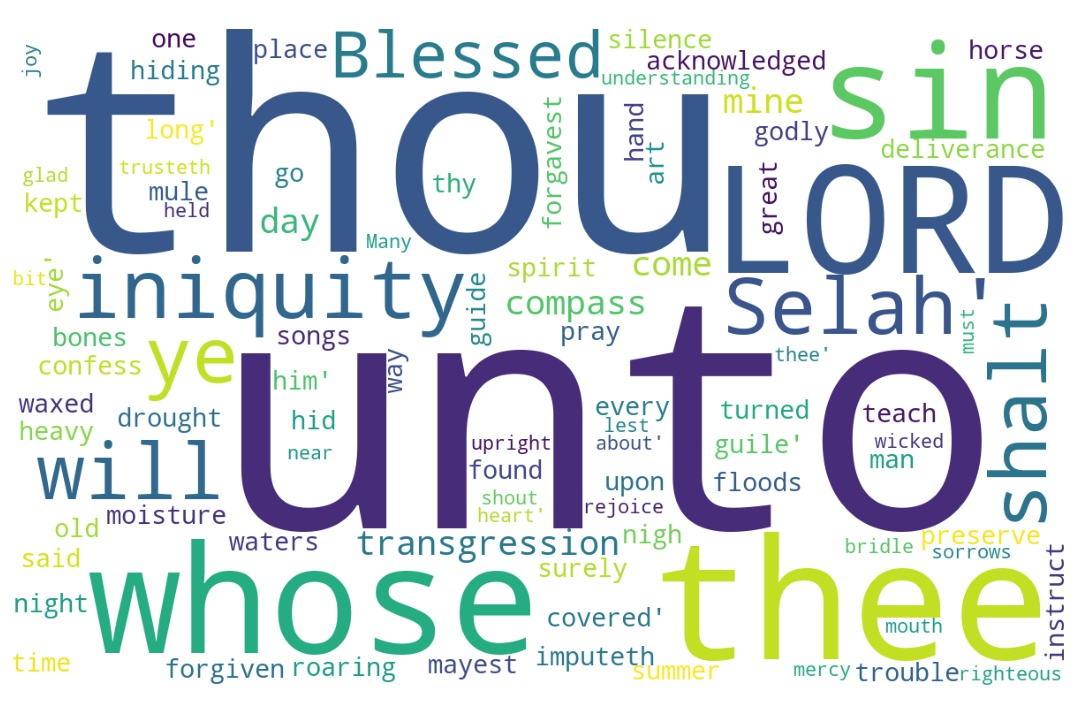
\includegraphics[width=\linewidth]{19OT-Psalms/Psalm32-WordCloud.jpg}
  \caption{Psalm 32 Word Cloud}
  \label{fig:Psalm 32 word Cloud}
\end{figure}

\marginpar{\scriptsize \centering \fcolorbox{bone}{lime}{\textbf{BECOMING BLESSED}}\\ (Psalm 32) 
\begin{compactenum}[I.][8]
    \item \textbf{Confirmation of Forgiveness} \index[scripture]{Psalms!Psa 032:01-02} (Psa 32:1-2)
    \item \textbf{Confession of Sin} \index[scripture]{Psalms!Psa 032:03-05} (Psa 32:3-5)
    \item \textbf{Counsel to a Saint} \index[scripture]{Psalms!Psa 032:06} (Psa 32:6)
    \item \textbf{Contentment in the Lord} \index[scripture]{Psalms!Psa 032:07-11} (Psa 32:7-11)
    \item \textbf{Correction to the Walk} \index[scripture]{Psalms!Psa 032:09} (Psa 32:9)
    \item \textbf{Conclusion to the Matter} \index[scripture]{Psalms!Psa 032:10-11} (Psa 32:10-11)
\end{compactenum} }


\marginpar{\scriptsize \centering \fcolorbox{bone}{yellow}{\textbf{WHEN GOD DELIVERS}}\\ (Psalm 32) 
\begin{compactenum}[I.][8]
    \item The \textbf{Sinner is Cleaned}
    \item The \textbf{Slate is Cleared}
    \item The \textbf{Sin is Covered}
    \item The \textbf{Sentence is Canceled}
    \item \textbf{Satisfaction is Created}
    \item A \textbf{Saint is Counselled}
    \item The \textbf{Storm is Calmed}
\end{compactenum} }

\marginpar{\scriptsize \centering \fcolorbox{bone}{black}{\textbf{\textcolor[cmyk]{0,0,0,0}{WHAT JESUS BECOMES}}}\\ (Psalm 32) 
 \begin{compactenum}[I.][8]
    \item The \textbf{Shelter in Distress}
    \item \textbf{Safety in Danger}
    \item The \textbf{Song of Deliverance}
    \item The \textbf{Shout in Despair}
    \item \textbf{Source of Delight}
    \item A \textbf{Supply in Drought}
    \item \textbf{Strength in Discouragement}
    \item A \textbf{Certain Dwelling-place}
\end{compactenum} }

\footnote{\textcolor[cmyk]{0.99998,1,0,0}{\hyperlink{TOC}{Return to end of Table of Contents.}}}\footnote{\href{https://www.audioverse.org/english/audiobibles/books/ENGKJV/O/Ps/1}{\textcolor[cmyk]{0.99998,1,0,0}{Psalms Audio}}}\textcolor[cmyk]{0.99998,1,0,0}{\emph{A Psalm} of David, Maschil.}\\
\\
\textcolor[cmyk]{0.99998,1,0,0}{Blessed \emph{is} \emph{he} \emph{whose} transgression \emph{is} \fcolorbox{bone}{lime}{forgiven}, \emph{whose} sin \emph{is} covered.}
[2] \textcolor[cmyk]{0.99998,1,0,0}{Blessed \emph{is} \fcolorbox{bone}{bone}{the} man unto whom \fcolorbox{bone}{bone}{the} LORD imputeth not iniquity, and in whose spirit \emph{there} \emph{is} no guile.}
[3] \textcolor[cmyk]{0.99998,1,0,0}{When I kept silence, my bones waxed old through my roaring all \fcolorbox{bone}{bone}{the} day long.}
[4] \textcolor[cmyk]{0.99998,1,0,0}{For day and night thy hand was heavy upon me: my moisture is turned into \fcolorbox{bone}{bone}{the} drought of summer. Selah.}
[5] \textcolor[cmyk]{0.99998,1,0,0}{I acknowledged my \fcolorbox{bone}{lime}{sin} unto thee, and mine iniquity have I not hid. I said, I will confess my transgressions unto \fcolorbox{bone}{bone}{the} LORD; and thou forgavest \fcolorbox{bone}{bone}{the} iniquity of my sin. Selah.}
[6] \textcolor[cmyk]{0.99998,1,0,0}{For this shall every one that is godly pray unto thee in a time when thou mayest be found: surely in \fcolorbox{bone}{bone}{the} floods of great waters \fcolorbox{bone}{lime}{they} shall not come nigh unto him.}
[7] \textcolor[cmyk]{0.99998,1,0,0}{Thou \emph{art} my \fcolorbox{bone}{lime}{hiding place}; thou shalt preserve me from trouble; thou shalt compass me about with songs of deliverance. Selah.}
[8] \textcolor[cmyk]{0.99998,1,0,0}{I will instruct thee and teach thee in \fcolorbox{bone}{bone}{the} way which thou shalt go: I will guide thee with mine eye.}
[9] \textcolor[cmyk]{0.99998,1,0,0}{Be ye not as \fcolorbox{bone}{bone}{the} horse, \emph{or} as \fcolorbox{bone}{bone}{the} mule, \emph{which} have no understanding: whose mouth must be \fcolorbox{bone}{lime}{held in} with bit and bridle, lest they come near unto thee.}
[10] \textcolor[cmyk]{0.99998,1,0,0}{Many sorrows \emph{shall} \emph{be} to \fcolorbox{bone}{bone}{the} wicked: but he that trusteth in \fcolorbox{bone}{bone}{the} LORD, \fcolorbox{bone}{lime}{mercy} shall compass him about.}
[11] \textcolor[cmyk]{0.99998,1,0,0}{Be glad in \fcolorbox{bone}{bone}{the} LORD, and rejoice, ye righteous: and shout for joy, all \emph{ye} \emph{that} \emph{are} upright in heart.}
\section{Psalm 32 Comments}

\subsection{Numeric Nuggets}
\textbf{13: } The word ``the'' is used 13 times in Psalm 32.  The 13-letter words ``transgression'' and ``understanding'' are used in the chapter. How to be blessed (37 references):
\begin{compactenum}
	\item Numbers 24:9 [19]
	\item Psalms 1:1 [1]
	\item Psalms 32:1 [1]
	\item Psalms 32:2 [1]
	\item Psalms 33:12 [1]
	\item Psalms 34:8 [10]
	\item Psalms 40:4 [1]
	\item Psalms 41:1 [1]
	\item Psalms 65:4 [1]
	\item Psalms 84:5 [1]
	\item Psalms 84:12 [5]
	\item Psalms 89:15 [1]
	\item Psalms 94:12 [1]
	\item Psalms 112:1 [5]
	\item Psalms 128:1 [1]
	\item Proverbs 8:34 [1]
	\item Isaiah 56:2 [1]
	\item Jeremiah 17:7 [1]
	\item Daniel 12:12 [1]
	\item  Matthew 11:6 [2]
	\item  Matthew 21:9 [18]
	\item  Matthew 23:39 [16]
	\item Matthew 24:46 [1]
	\item Mark 11:9 [13]
	\item Luke 1:42 [17]
	\item Luke 1:45 [2]
	\item Luke 7:23 [2]
	\item Luke 11:27 [25]
	\item Luke 12:43 [1]
	\item Luke 13:35 [28]
	\item Luke 14:15 [19]
	\item John 12:13 - the King of Israel that  coming the in the name of the Lord
	\item Romans 4:8 - not being imputed sin
	\item James 1:12 - enduring temptation
	\item Revelation 1:3 - read and heed the words of Revelation
	\item Revelation 16:15 - watch for the Lord and ``keeps his garments'' [clean]
	\item Revelation 22:7 - keep the sayings of the book
\end{compactenum}


%\index[NWIV]{11!Psalms!Psa 32:1}\index[AWIP]{Blessed!Psalms!Psa 32:1}\index[AWIP]{\emph{is}!Psalms!Psa 32:1}\index[AWIP]{\emph{is}!Psalms!Psa 32:1 (2)}\index[AWIP]{\emph{is}!Psalms!Psa 32:1 (3)}\index[AWIP]{\emph{he}!Psalms!Psa 32:1}\index[AWIP]{\emph{whose}!Psalms!Psa 32:1}\index[AWIP]{\emph{whose}!Psalms!Psa 32:1 (2)}\index[AWIP]{transgression!Psalms!Psa 32:1}\index[AWIP]{forgiven!Psalms!Psa 32:1}\index[AWIP]{sin!Psalms!Psa 32:1}\index[AWIP]{covered!Psalms!Psa 32:1}\index[AWIP]{\emph{is}!Psalms!Psa 32:1}\index[AWIP]{\emph{is}!Psalms!Psa 32:1 (2)}\index[AWIP]{\emph{is}!Psalms!Psa 32:1 (3)}\index[AWIP]{\emph{he}!Psalms!Psa 32:1}\index[AWIP]{\emph{whose}!Psalms!Psa 32:1}\index[AWIP]{\emph{whose}!Psalms!Psa 32:1 (2)}

\index[NWIV]{19!Psalms!Psa 32:2}\index[AWIP]{Blessed!Psalms!Psa 32:2}\index[AWIP]{\emph{is}!Psalms!Psa 32:2}\index[AWIP]{\emph{is}!Psalms!Psa 32:2 (2)}\index[AWIP]{the!Psalms!Psa 32:2}\index[AWIP]{the!Psalms!Psa 32:2 (2)}\index[AWIP]{man!Psalms!Psa 32:2}\index[AWIP]{unto!Psalms!Psa 32:2}\index[AWIP]{whom!Psalms!Psa 32:2}\index[AWIP]{LORD!Psalms!Psa 32:2}\index[AWIP]{imputeth!Psalms!Psa 32:2}\index[AWIP]{not!Psalms!Psa 32:2}\index[AWIP]{iniquity!Psalms!Psa 32:2}\index[AWIP]{and!Psalms!Psa 32:2}\index[AWIP]{in!Psalms!Psa 32:2}\index[AWIP]{whose!Psalms!Psa 32:2}\index[AWIP]{spirit!Psalms!Psa 32:2}\index[AWIP]{\emph{there}!Psalms!Psa 32:2}\index[AWIP]{no!Psalms!Psa 32:2}\index[AWIP]{guile!Psalms!Psa 32:2}\index[AWIP]{\emph{is}!Psalms!Psa 32:2}\index[AWIP]{\emph{is}!Psalms!Psa 32:2 (2)}\index[AWIP]{\emph{there}!Psalms!Psa 32:2}

\index[NWIV]{15!Psalms!Psa 32:3}\index[AWIP]{When!Psalms!Psa 32:3}\index[AWIP]{I!Psalms!Psa 32:3}\index[AWIP]{kept!Psalms!Psa 32:3}\index[AWIP]{silence!Psalms!Psa 32:3}\index[AWIP]{my!Psalms!Psa 32:3}\index[AWIP]{my!Psalms!Psa 32:3 (2)}\index[AWIP]{bones!Psalms!Psa 32:3}\index[AWIP]{waxed!Psalms!Psa 32:3}\index[AWIP]{old!Psalms!Psa 32:3}\index[AWIP]{through!Psalms!Psa 32:3}\index[AWIP]{roaring!Psalms!Psa 32:3}\index[AWIP]{all!Psalms!Psa 32:3}\index[AWIP]{the!Psalms!Psa 32:3}\index[AWIP]{day!Psalms!Psa 32:3}\index[AWIP]{long!Psalms!Psa 32:3}

\index[NWIV]{20!Psalms!Psa 32:4}\index[AWIP]{For!Psalms!Psa 32:4}\index[AWIP]{day!Psalms!Psa 32:4}\index[AWIP]{and!Psalms!Psa 32:4}\index[AWIP]{night!Psalms!Psa 32:4}\index[AWIP]{thy!Psalms!Psa 32:4}\index[AWIP]{hand!Psalms!Psa 32:4}\index[AWIP]{was!Psalms!Psa 32:4}\index[AWIP]{heavy!Psalms!Psa 32:4}\index[AWIP]{upon!Psalms!Psa 32:4}\index[AWIP]{me!Psalms!Psa 32:4}\index[AWIP]{my!Psalms!Psa 32:4}\index[AWIP]{moisture!Psalms!Psa 32:4}\index[AWIP]{is!Psalms!Psa 32:4}\index[AWIP]{turned!Psalms!Psa 32:4}\index[AWIP]{into!Psalms!Psa 32:4}\index[AWIP]{the!Psalms!Psa 32:4}\index[AWIP]{drought!Psalms!Psa 32:4}\index[AWIP]{of!Psalms!Psa 32:4}\index[AWIP]{summer!Psalms!Psa 32:4}\index[AWIP]{Selah!Psalms!Psa 32:4}

\index[NWIV]{32!Psalms!Psa 32:5}\index[AWIP]{I!Psalms!Psa 32:5}\index[AWIP]{I!Psalms!Psa 32:5 (2)}\index[AWIP]{I!Psalms!Psa 32:5 (3)}\index[AWIP]{I!Psalms!Psa 32:5 (4)}\index[AWIP]{acknowledged!Psalms!Psa 32:5}\index[AWIP]{my!Psalms!Psa 32:5}\index[AWIP]{my!Psalms!Psa 32:5 (2)}\index[AWIP]{my!Psalms!Psa 32:5 (3)}\index[AWIP]{sin!Psalms!Psa 32:5}\index[AWIP]{sin!Psalms!Psa 32:5 (2)}\index[AWIP]{unto!Psalms!Psa 32:5}\index[AWIP]{unto!Psalms!Psa 32:5 (2)}\index[AWIP]{thee!Psalms!Psa 32:5}\index[AWIP]{and!Psalms!Psa 32:5}\index[AWIP]{and!Psalms!Psa 32:5 (2)}\index[AWIP]{mine!Psalms!Psa 32:5}\index[AWIP]{iniquity!Psalms!Psa 32:5}\index[AWIP]{iniquity!Psalms!Psa 32:5 (2)}\index[AWIP]{have!Psalms!Psa 32:5}\index[AWIP]{not!Psalms!Psa 32:5}\index[AWIP]{hid!Psalms!Psa 32:5}\index[AWIP]{said!Psalms!Psa 32:5}\index[AWIP]{will!Psalms!Psa 32:5}\index[AWIP]{confess!Psalms!Psa 32:5}\index[AWIP]{transgressions!Psalms!Psa 32:5}\index[AWIP]{the!Psalms!Psa 32:5}\index[AWIP]{the!Psalms!Psa 32:5 (2)}\index[AWIP]{LORD!Psalms!Psa 32:5}\index[AWIP]{thou!Psalms!Psa 32:5}\index[AWIP]{forgavest!Psalms!Psa 32:5}\index[AWIP]{of!Psalms!Psa 32:5}\index[AWIP]{Selah!Psalms!Psa 32:5}

\index[NWIV]{33!Psalms!Psa 32:6}\index[AWIP]{For!Psalms!Psa 32:6}\index[AWIP]{this!Psalms!Psa 32:6}\index[AWIP]{shall!Psalms!Psa 32:6}\index[AWIP]{shall!Psalms!Psa 32:6 (2)}\index[AWIP]{every!Psalms!Psa 32:6}\index[AWIP]{one!Psalms!Psa 32:6}\index[AWIP]{that!Psalms!Psa 32:6}\index[AWIP]{is!Psalms!Psa 32:6}\index[AWIP]{godly!Psalms!Psa 32:6}\index[AWIP]{pray!Psalms!Psa 32:6}\index[AWIP]{unto!Psalms!Psa 32:6}\index[AWIP]{unto!Psalms!Psa 32:6 (2)}\index[AWIP]{thee!Psalms!Psa 32:6}\index[AWIP]{in!Psalms!Psa 32:6}\index[AWIP]{in!Psalms!Psa 32:6 (2)}\index[AWIP]{a!Psalms!Psa 32:6}\index[AWIP]{time!Psalms!Psa 32:6}\index[AWIP]{when!Psalms!Psa 32:6}\index[AWIP]{thou!Psalms!Psa 32:6}\index[AWIP]{mayest!Psalms!Psa 32:6}\index[AWIP]{be!Psalms!Psa 32:6}\index[AWIP]{found!Psalms!Psa 32:6}\index[AWIP]{surely!Psalms!Psa 32:6}\index[AWIP]{the!Psalms!Psa 32:6}\index[AWIP]{floods!Psalms!Psa 32:6}\index[AWIP]{of!Psalms!Psa 32:6}\index[AWIP]{great!Psalms!Psa 32:6}\index[AWIP]{waters!Psalms!Psa 32:6}\index[AWIP]{they!Psalms!Psa 32:6}\index[AWIP]{not!Psalms!Psa 32:6}\index[AWIP]{come!Psalms!Psa 32:6}\index[AWIP]{nigh!Psalms!Psa 32:6}\index[AWIP]{him!Psalms!Psa 32:6}

\index[NWIV]{21!Psalms!Psa 32:7}\index[AWIP]{Thou!Psalms!Psa 32:7}\index[AWIP]{\emph{art}!Psalms!Psa 32:7}\index[AWIP]{my!Psalms!Psa 32:7}\index[AWIP]{hiding!Psalms!Psa 32:7}\index[AWIP]{place!Psalms!Psa 32:7}\index[AWIP]{thou!Psalms!Psa 32:7}\index[AWIP]{thou!Psalms!Psa 32:7 (2)}\index[AWIP]{shalt!Psalms!Psa 32:7}\index[AWIP]{shalt!Psalms!Psa 32:7 (2)}\index[AWIP]{preserve!Psalms!Psa 32:7}\index[AWIP]{me!Psalms!Psa 32:7}\index[AWIP]{me!Psalms!Psa 32:7 (2)}\index[AWIP]{from!Psalms!Psa 32:7}\index[AWIP]{trouble!Psalms!Psa 32:7}\index[AWIP]{compass!Psalms!Psa 32:7}\index[AWIP]{about!Psalms!Psa 32:7}\index[AWIP]{with!Psalms!Psa 32:7}\index[AWIP]{songs!Psalms!Psa 32:7}\index[AWIP]{of!Psalms!Psa 32:7}\index[AWIP]{deliverance!Psalms!Psa 32:7}\index[AWIP]{Selah!Psalms!Psa 32:7}\index[AWIP]{\emph{art}!Psalms!Psa 32:7}

\index[NWIV]{21!Psalms!Psa 32:8}\index[AWIP]{I!Psalms!Psa 32:8}\index[AWIP]{I!Psalms!Psa 32:8 (2)}\index[AWIP]{will!Psalms!Psa 32:8}\index[AWIP]{will!Psalms!Psa 32:8 (2)}\index[AWIP]{instruct!Psalms!Psa 32:8}\index[AWIP]{thee!Psalms!Psa 32:8}\index[AWIP]{thee!Psalms!Psa 32:8 (2)}\index[AWIP]{thee!Psalms!Psa 32:8 (3)}\index[AWIP]{and!Psalms!Psa 32:8}\index[AWIP]{teach!Psalms!Psa 32:8}\index[AWIP]{in!Psalms!Psa 32:8}\index[AWIP]{the!Psalms!Psa 32:8}\index[AWIP]{way!Psalms!Psa 32:8}\index[AWIP]{which!Psalms!Psa 32:8}\index[AWIP]{thou!Psalms!Psa 32:8}\index[AWIP]{shalt!Psalms!Psa 32:8}\index[AWIP]{go!Psalms!Psa 32:8}\index[AWIP]{guide!Psalms!Psa 32:8}\index[AWIP]{with!Psalms!Psa 32:8}\index[AWIP]{mine!Psalms!Psa 32:8}\index[AWIP]{eye!Psalms!Psa 32:8}

\index[NWIV]{30!Psalms!Psa 32:9}\index[AWIP]{Be!Psalms!Psa 32:9}\index[AWIP]{ye!Psalms!Psa 32:9}\index[AWIP]{not!Psalms!Psa 32:9}\index[AWIP]{as!Psalms!Psa 32:9}\index[AWIP]{as!Psalms!Psa 32:9 (2)}\index[AWIP]{the!Psalms!Psa 32:9}\index[AWIP]{the!Psalms!Psa 32:9 (2)}\index[AWIP]{horse!Psalms!Psa 32:9}\index[AWIP]{\emph{or}!Psalms!Psa 32:9}\index[AWIP]{mule!Psalms!Psa 32:9}\index[AWIP]{\emph{which}!Psalms!Psa 32:9}\index[AWIP]{have!Psalms!Psa 32:9}\index[AWIP]{no!Psalms!Psa 32:9}\index[AWIP]{understanding!Psalms!Psa 32:9}\index[AWIP]{whose!Psalms!Psa 32:9}\index[AWIP]{mouth!Psalms!Psa 32:9}\index[AWIP]{must!Psalms!Psa 32:9}\index[AWIP]{be!Psalms!Psa 32:9}\index[AWIP]{held!Psalms!Psa 32:9}\index[AWIP]{in!Psalms!Psa 32:9}\index[AWIP]{with!Psalms!Psa 32:9}\index[AWIP]{bit!Psalms!Psa 32:9}\index[AWIP]{and!Psalms!Psa 32:9}\index[AWIP]{bridle!Psalms!Psa 32:9}\index[AWIP]{lest!Psalms!Psa 32:9}\index[AWIP]{they!Psalms!Psa 32:9}\index[AWIP]{come!Psalms!Psa 32:9}\index[AWIP]{near!Psalms!Psa 32:9}\index[AWIP]{unto!Psalms!Psa 32:9}\index[AWIP]{thee!Psalms!Psa 32:9}\index[AWIP]{\emph{or}!Psalms!Psa 32:9}\index[AWIP]{\emph{which}!Psalms!Psa 32:9}

\index[NWIV]{19!Psalms!Psa 32:10}\index[AWIP]{Many!Psalms!Psa 32:10}\index[AWIP]{sorrows!Psalms!Psa 32:10}\index[AWIP]{\emph{shall}!Psalms!Psa 32:10}\index[AWIP]{\emph{be}!Psalms!Psa 32:10}\index[AWIP]{to!Psalms!Psa 32:10}\index[AWIP]{the!Psalms!Psa 32:10}\index[AWIP]{the!Psalms!Psa 32:10 (2)}\index[AWIP]{wicked!Psalms!Psa 32:10}\index[AWIP]{but!Psalms!Psa 32:10}\index[AWIP]{he!Psalms!Psa 32:10}\index[AWIP]{that!Psalms!Psa 32:10}\index[AWIP]{trusteth!Psalms!Psa 32:10}\index[AWIP]{in!Psalms!Psa 32:10}\index[AWIP]{LORD!Psalms!Psa 32:10}\index[AWIP]{mercy!Psalms!Psa 32:10}\index[AWIP]{shall!Psalms!Psa 32:10}\index[AWIP]{compass!Psalms!Psa 32:10}\index[AWIP]{him!Psalms!Psa 32:10}\index[AWIP]{about!Psalms!Psa 32:10}\index[AWIP]{\emph{shall}!Psalms!Psa 32:10}\index[AWIP]{\emph{be}!Psalms!Psa 32:10}

\index[NWIV]{20!Psalms!Psa 32:11}\index[AWIP]{Be!Psalms!Psa 32:11}\index[AWIP]{glad!Psalms!Psa 32:11}\index[AWIP]{in!Psalms!Psa 32:11}\index[AWIP]{in!Psalms!Psa 32:11 (2)}\index[AWIP]{the!Psalms!Psa 32:11}\index[AWIP]{LORD!Psalms!Psa 32:11}\index[AWIP]{and!Psalms!Psa 32:11}\index[AWIP]{and!Psalms!Psa 32:11 (2)}\index[AWIP]{rejoice!Psalms!Psa 32:11}\index[AWIP]{ye!Psalms!Psa 32:11}\index[AWIP]{righteous!Psalms!Psa 32:11}\index[AWIP]{shout!Psalms!Psa 32:11}\index[AWIP]{for!Psalms!Psa 32:11}\index[AWIP]{joy!Psalms!Psa 32:11}\index[AWIP]{all!Psalms!Psa 32:11}\index[AWIP]{\emph{ye}!Psalms!Psa 32:11}\index[AWIP]{\emph{that}!Psalms!Psa 32:11}\index[AWIP]{\emph{are}!Psalms!Psa 32:11}\index[AWIP]{upright!Psalms!Psa 32:11}\index[AWIP]{heart!Psalms!Psa 32:11}\index[AWIP]{\emph{ye}!Psalms!Psa 32:11}\index[AWIP]{\emph{that}!Psalms!Psa 32:11}\index[AWIP]{\emph{are}!Psalms!Psa 32:11}


\section{Psalm 32 Outlines}

\subsection{My Outlines}

\subsubsection{Becoming Blessed}
%Psalm 32:\footnote{unknown, Keith Anthony}
\index[speaker]{Keith Anthony!Psalm 032 (Becoming Blessed)}
\index[series]{Psalms (Keith Anthony)!Psalm 032 (Becoming Blessed)}
\index[date]{2016/07/08!Psalm 032 (Becoming Blessed) (Keith Anthony)}
\begin{compactenum}[I.]
    \item \textbf{Confirmation of Forgiveness} \index[scripture]{Psalms!Psa 032:01-02} (Psa 32:1-2)
    \item \textbf{Confession of Sin} \index[scripture]{Psalms!Psa 032:03-05} (Psa 32:3-5)
    \item \textbf{Counsel to a Saint} \index[scripture]{Psalms!Psa 032:06} (Psa 32:6)
    \item \textbf{Contentment in the Lord} \index[scripture]{Psalms!Psa 032:07-11} (Psa 32:7-11)
    \item \textbf{Correction to the Walk} \index[scripture]{Psalms!Psa 032:09} (Psa 32:9)
    \item \textbf{Conclusion to the Matter} \index[scripture]{Psalms!Psa 032:10-11} (Psa 32:10-11)
\end{compactenum}

\subsubsection{What Happens when God Delivers}
\index[speaker]{Keith Anthony!Psalm 032 (What Happens when God Delivers)}
\index[series]{Psalms (Keith Anthony)!Psalm 032 (What Happens when God Delivers)}
\index[date]{2014/12/01!Psalm 032 (What Happens when God Delivers) (Keith Anthony)}
\textbf{Introduction: }Psalm 32 records rejoicing of a man who has been delivered:
\begin{compactenum}[I.]
    \item The \textbf{Sinner is Cleaned}
    \item The \textbf{Slate is Cleared}
    \item The \textbf{Sin is Covered}
    \item The \textbf{Sentence is Canceled}
    \item \textbf{Satisfaction is Created}
    \item A \textbf{Saint is Counselled}
    \item The \textbf{Storm is Calmed}
\end{compactenum}

\subsubsection{What Jesus Becomes}
\index[speaker]{Keith Anthony!Psalm 032 (What Jesus Becomes)}
\index[series]{Psalms (Keith Anthony)!Psalm 032 (What Jesus Becomes)}
\index[date]{2014/12/01!Psalm 032 (What Jesus Becomes) (Keith Anthony)}
\textbf{Introduction: }For the saved man Psalm 32 shows what Jesus becomes to him:
\begin{compactenum}[I.]
    \item The \textbf{Shelter in Distress}
    \item \textbf{Safety in Danger}
    \item The \textbf{Song of Deliverance}
    \item The \textbf{Shout in Despair}
    \item \textbf{Source of Delight}
    \item A \textbf{Supply in Drought}
    \item \textbf{Strength in Discouragement}
    \item A \textbf{Certain Dwelling-place}
\end{compactenum}

\subsection{Outlines from Others}




%\section{Psalm 32 Statistics}

%%%%%%%%%%%%%%%%%%%%%%%%%%%
%%%%% Word Statistics
%%%%%%%%%%%%%%%%%%%%%%%%%%


\normalsize



\subsection{Chapter Word Statistics}


%%%%%%%%%%
%%%%%%%%%%
 
\begin{center}
\begin{longtable}{l|c|c|c|c}
\caption[Stats for Psalm 32]{Stats for Psalm 32} \label{table:Stats for Psalm 32} \\ 
\hline \multicolumn{1}{|c|}{\textbf{Verse(s)}} & \multicolumn{1}{|c|}{\textbf{Count}} & \multicolumn{1}{|c|}{\textbf{Unique}} & \multicolumn{1}{|c|}{\textbf{Italics}} & \multicolumn{1}{|c|}{\textbf{Uniq Italic}}  \\ \hline 
\endfirsthead
 
\multicolumn{5}{c}
{{\bfseries \tablename\ \thetable{} -- continued from previous page}} \\  
\hline \multicolumn{1}{|c|}{\textbf{Verse(s)}} & \multicolumn{1}{|c|}{\textbf{Count}} & \multicolumn{1}{|c|}{\textbf{Unique}} & \multicolumn{1}{|c|}{\textbf{Italics}} & \multicolumn{1}{|c|}{\textbf{Uniq Italic}}  \\ \hline 
\endhead
 
\hline \multicolumn{5}{|r|}{{Continued if needed}} \\ \hline
\endfoot 
1 & 11 & 8 & 6 & 3\\ \hline
2 & 19 & 17 & 3 & 2\\ \hline
3 & 15 & 14 & 0 & 0\\ \hline
4 & 20 & 20 & 0 & 0\\ \hline
5 & 32 & 22 & 0 & 0\\ \hline
6 & 33 & 30 & 0 & 0\\ \hline
7 & 21 & 18 & 1 & 1\\ \hline
8 & 21 & 17 & 0 & 0\\ \hline
9 & 30 & 28 & 2 & 2\\ \hline
10 & 19 & 18 & 2 & 2\\ \hline
11 & 20 & 18 & 3 & 3\\ \hline
\hline \hline
Total & 241 & 140 & 17 & 12



\end{longtable}
\end{center}

%%%%%%%%%%
%%%%%%%%%%
 
\subsection{Words by Frequency}

\begin{center}
\begin{longtable}{l|r}
\caption[Word Frequencies in Psalm 32]{Word Frequencies in Psalm 32} \label{table:WordsIn-Psalm-32} \\ 
\hline \multicolumn{1}{|c|}{\textbf{Word}} & \multicolumn{1}{c|}{\textbf{Frequency}} \\ \hline 
\endfirsthead
 
\multicolumn{2}{c}
{{\bfseries \tablename\ \thetable{} -- continued from previous page}} \\ 
\hline \multicolumn{1}{|c|}{\textbf{Word}} & \multicolumn{1}{c|}{\textbf{Frequency}} \\ \hline 
\endhead
 
\hline \multicolumn{2}{|r|}{{Continued if needed}} \\ \hline
\endfoot
 
\hline \hline
\endlastfoot
the & 13 \\ \hline
and & 8 \\ \hline
in & 8 \\ \hline
I & 7 \\ \hline
my & 7 \\ \hline
unto & 6 \\ \hline
thee & 6 \\ \hline
\emph{is} & 5 \\ \hline
thou & 5 \\ \hline
LORD & 4 \\ \hline
not & 4 \\ \hline
of & 4 \\ \hline
sin & 3 \\ \hline
iniquity & 3 \\ \hline
me & 3 \\ \hline
Selah & 3 \\ \hline
will & 3 \\ \hline
shall & 3 \\ \hline
shalt & 3 \\ \hline
with & 3 \\ \hline
Blessed & 2 \\ \hline
\emph{whose} & 2 \\ \hline
whose & 2 \\ \hline
no & 2 \\ \hline
all & 2 \\ \hline
day & 2 \\ \hline
For & 2 \\ \hline
is & 2 \\ \hline
mine & 2 \\ \hline
have & 2 \\ \hline
that & 2 \\ \hline
be & 2 \\ \hline
they & 2 \\ \hline
come & 2 \\ \hline
him & 2 \\ \hline
compass & 2 \\ \hline
about & 2 \\ \hline
Be & 2 \\ \hline
ye & 2 \\ \hline
as & 2 \\ \hline
\emph{he} & 1 \\ \hline
transgression & 1 \\ \hline
forgiven & 1 \\ \hline
covered & 1 \\ \hline
man & 1 \\ \hline
whom & 1 \\ \hline
imputeth & 1 \\ \hline
spirit & 1 \\ \hline
\emph{there} & 1 \\ \hline
guile & 1 \\ \hline
When & 1 \\ \hline
kept & 1 \\ \hline
silence & 1 \\ \hline
bones & 1 \\ \hline
waxed & 1 \\ \hline
old & 1 \\ \hline
through & 1 \\ \hline
roaring & 1 \\ \hline
long & 1 \\ \hline
night & 1 \\ \hline
thy & 1 \\ \hline
hand & 1 \\ \hline
was & 1 \\ \hline
heavy & 1 \\ \hline
upon & 1 \\ \hline
moisture & 1 \\ \hline
turned & 1 \\ \hline
into & 1 \\ \hline
drought & 1 \\ \hline
summer & 1 \\ \hline
acknowledged & 1 \\ \hline
hid & 1 \\ \hline
said & 1 \\ \hline
confess & 1 \\ \hline
transgressions & 1 \\ \hline
forgavest & 1 \\ \hline
this & 1 \\ \hline
every & 1 \\ \hline
one & 1 \\ \hline
godly & 1 \\ \hline
pray & 1 \\ \hline
a & 1 \\ \hline
time & 1 \\ \hline
when & 1 \\ \hline
mayest & 1 \\ \hline
found & 1 \\ \hline
surely & 1 \\ \hline
floods & 1 \\ \hline
great & 1 \\ \hline
waters & 1 \\ \hline
nigh & 1 \\ \hline
Thou & 1 \\ \hline
\emph{art} & 1 \\ \hline
hiding & 1 \\ \hline
place & 1 \\ \hline
preserve & 1 \\ \hline
from & 1 \\ \hline
trouble & 1 \\ \hline
songs & 1 \\ \hline
deliverance & 1 \\ \hline
instruct & 1 \\ \hline
teach & 1 \\ \hline
way & 1 \\ \hline
which & 1 \\ \hline
go & 1 \\ \hline
guide & 1 \\ \hline
eye & 1 \\ \hline
horse & 1 \\ \hline
\emph{or} & 1 \\ \hline
mule & 1 \\ \hline
\emph{which} & 1 \\ \hline
understanding & 1 \\ \hline
mouth & 1 \\ \hline
must & 1 \\ \hline
held & 1 \\ \hline
bit & 1 \\ \hline
bridle & 1 \\ \hline
lest & 1 \\ \hline
near & 1 \\ \hline
Many & 1 \\ \hline
sorrows & 1 \\ \hline
\emph{shall} & 1 \\ \hline
\emph{be} & 1 \\ \hline
to & 1 \\ \hline
wicked & 1 \\ \hline
but & 1 \\ \hline
he & 1 \\ \hline
trusteth & 1 \\ \hline
mercy & 1 \\ \hline
glad & 1 \\ \hline
rejoice & 1 \\ \hline
righteous & 1 \\ \hline
shout & 1 \\ \hline
for & 1 \\ \hline
joy & 1 \\ \hline
\emph{ye} & 1 \\ \hline
\emph{that} & 1 \\ \hline
\emph{are} & 1 \\ \hline
upright & 1 \\ \hline
heart & 1 \\ \hline
\end{longtable}
\end{center}



\normalsize



\subsection{Words Alphabetically}
\scriptsize\begin{center}
\begin{longtable}{l|r}
\caption[Word Alphabetically in Psalm 32]{Word Alphabetically in Psalm 32} \label{table:WordsIn-Psalm-32} \\ 
\hline \multicolumn{1}{|c|}{\textbf{Word}} & \multicolumn{1}{c|}{\textbf{Frequency}} \\ \hline 
\endfirsthead
 
\multicolumn{2}{c}
{{\bfseries \tablename\ \thetable{} -- continued from previous page}} \\ 
\hline \multicolumn{1}{|c|}{\textbf{Word}} & \multicolumn{1}{c|}{\textbf{Frequency}} \\ \hline 
\endhead
 
\hline \multicolumn{2}{|r|}{{Continued if needed}} \\ \hline
\endfoot
 
\hline \hline
\endlastfoot
Be & 2 \\ \hline
Blessed & 2 \\ \hline
For & 2 \\ \hline
I & 7 \\ \hline
LORD & 4 \\ \hline
Many & 1 \\ \hline
Selah & 3 \\ \hline
Thou & 1 \\ \hline
When & 1 \\ \hline
\emph{are} & 1 \\ \hline
\emph{art} & 1 \\ \hline
\emph{be} & 1 \\ \hline
\emph{he} & 1 \\ \hline
\emph{is} & 5 \\ \hline
\emph{or} & 1 \\ \hline
\emph{shall} & 1 \\ \hline
\emph{that} & 1 \\ \hline
\emph{there} & 1 \\ \hline
\emph{which} & 1 \\ \hline
\emph{whose} & 2 \\ \hline
\emph{ye} & 1 \\ \hline
a & 1 \\ \hline
about & 2 \\ \hline
acknowledged & 1 \\ \hline
all & 2 \\ \hline
and & 8 \\ \hline
as & 2 \\ \hline
be & 2 \\ \hline
bit & 1 \\ \hline
bones & 1 \\ \hline
bridle & 1 \\ \hline
but & 1 \\ \hline
come & 2 \\ \hline
compass & 2 \\ \hline
confess & 1 \\ \hline
covered & 1 \\ \hline
day & 2 \\ \hline
deliverance & 1 \\ \hline
drought & 1 \\ \hline
every & 1 \\ \hline
eye & 1 \\ \hline
floods & 1 \\ \hline
for & 1 \\ \hline
forgavest & 1 \\ \hline
forgiven & 1 \\ \hline
found & 1 \\ \hline
from & 1 \\ \hline
glad & 1 \\ \hline
go & 1 \\ \hline
godly & 1 \\ \hline
great & 1 \\ \hline
guide & 1 \\ \hline
guile & 1 \\ \hline
hand & 1 \\ \hline
have & 2 \\ \hline
he & 1 \\ \hline
heart & 1 \\ \hline
heavy & 1 \\ \hline
held & 1 \\ \hline
hid & 1 \\ \hline
hiding & 1 \\ \hline
him & 2 \\ \hline
horse & 1 \\ \hline
imputeth & 1 \\ \hline
in & 8 \\ \hline
iniquity & 3 \\ \hline
instruct & 1 \\ \hline
into & 1 \\ \hline
is & 2 \\ \hline
joy & 1 \\ \hline
kept & 1 \\ \hline
lest & 1 \\ \hline
long & 1 \\ \hline
man & 1 \\ \hline
mayest & 1 \\ \hline
me & 3 \\ \hline
mercy & 1 \\ \hline
mine & 2 \\ \hline
moisture & 1 \\ \hline
mouth & 1 \\ \hline
mule & 1 \\ \hline
must & 1 \\ \hline
my & 7 \\ \hline
near & 1 \\ \hline
nigh & 1 \\ \hline
night & 1 \\ \hline
no & 2 \\ \hline
not & 4 \\ \hline
of & 4 \\ \hline
old & 1 \\ \hline
one & 1 \\ \hline
place & 1 \\ \hline
pray & 1 \\ \hline
preserve & 1 \\ \hline
rejoice & 1 \\ \hline
righteous & 1 \\ \hline
roaring & 1 \\ \hline
said & 1 \\ \hline
shall & 3 \\ \hline
shalt & 3 \\ \hline
shout & 1 \\ \hline
silence & 1 \\ \hline
sin & 3 \\ \hline
songs & 1 \\ \hline
sorrows & 1 \\ \hline
spirit & 1 \\ \hline
summer & 1 \\ \hline
surely & 1 \\ \hline
teach & 1 \\ \hline
that & 2 \\ \hline
the & 13 \\ \hline
thee & 6 \\ \hline
they & 2 \\ \hline
this & 1 \\ \hline
thou & 5 \\ \hline
through & 1 \\ \hline
thy & 1 \\ \hline
time & 1 \\ \hline
to & 1 \\ \hline
transgression & 1 \\ \hline
transgressions & 1 \\ \hline
trouble & 1 \\ \hline
trusteth & 1 \\ \hline
turned & 1 \\ \hline
understanding & 1 \\ \hline
unto & 6 \\ \hline
upon & 1 \\ \hline
upright & 1 \\ \hline
was & 1 \\ \hline
waters & 1 \\ \hline
waxed & 1 \\ \hline
way & 1 \\ \hline
when & 1 \\ \hline
which & 1 \\ \hline
whom & 1 \\ \hline
whose & 2 \\ \hline
wicked & 1 \\ \hline
will & 3 \\ \hline
with & 3 \\ \hline
ye & 2 \\ \hline
\end{longtable}
\end{center}



\normalsize



\subsection{Word Lengths in Chapter}
\normalsize
\begin{longtable}{l|p{3.75in}}
\caption[Words by Length in Psalm 32]{Words by Length in Psalm 32} \label{table:WordsIn-Psalm-32} \\ 
\hline \multicolumn{1}{|c|}{\textbf{Length}} & \multicolumn{1}{c|}{\textbf{Words}} \\ \hline 
\endfirsthead
 
\multicolumn{2}{c}
{{\bfseries \tablename\ \thetable{} -- continued from previous page}} \\ 
\hline \multicolumn{1}{|c|}{\textbf{Length}} & \multicolumn{1}{c|}{\textbf{Words}} \\ \hline 
\endhead
 
\hline \multicolumn{2}{|r|}{{Continued if needed}} \\ \hline
\endfoot
 
\hline \hline
\endlastfoot
1 & I, a \\ \hline
2 & \emph{is}, \emph{he}, in, no, my, me, is, of, be, go, Be, ye, as, \emph{or}, \emph{be}, to, he, \emph{ye} \\ \hline
3 & sin, the, man, not, and, old, all, day, For, thy, was, hid, one, him, \emph{art}, way, eye, bit, but, for, joy, \emph{are} \\ \hline
4 & unto, whom, LORD, When, kept, long, hand, upon, into, thee, mine, have, said, will, thou, this, that, pray, time, when, they, come, nigh, Thou, from, with, mule, must, held, lest, near, Many, glad, \emph{that} \\ \hline
5 & \emph{whose}, whose, \emph{there}, guile, bones, waxed, night, heavy, Selah, shall, every, godly, found, great, place, shalt, about, songs, teach, which, guide, horse, \emph{which}, mouth, \emph{shall}, mercy, shout, heart \\ \hline
6 & spirit, turned, summer, mayest, surely, floods, waters, hiding, bridle, wicked \\ \hline
7 & Blessed, covered, silence, through, roaring, drought, confess, trouble, compass, sorrows, rejoice, upright \\ \hline
8 & forgiven, imputeth, iniquity, moisture, preserve, instruct, trusteth \\ \hline
9 & forgavest, righteous \\ \hline
11 & deliverance \\ \hline
12 & acknowledged \\ \hline
13 & transgression, understanding \\ \hline
14 & transgressions \\ \hline
\end{longtable}






%%%%%%%%%%
%%%%%%%%%%
\subsection{Psalm 32 Repeated Phrases}


%%%%%%%%%%
%%%%%%%%%%
\normalsize
 
\begin{center}
\begin{longtable}{|p{3.0in}|p{0.5in}|}
\caption[Psalm 32 Repeated Phrases]{Psalm 32 Repeated Phrases}\label{table:Repeated Phrases Psalm 32} \\
\hline \multicolumn{1}{|c|}{\textbf{Phrase}} & \multicolumn{1}{c|}{\textbf{Frequency}} \\ \hline 
\endfirsthead
 
\multicolumn{2}{c}
{{\bfseries \tablename\ \thetable{} -- continued from previous page}} \\  
\hline \multicolumn{1}{|c|}{\textbf{Phrase}} & \multicolumn{1}{c|}{\textbf{Frequency}} \\ \hline 
\endhead
 
\hline \multicolumn{2}{c}{{ }} \\ \hline
\endfoot 
the LORD & 4\\ \hline 
in the & 4\\ \hline 
unto thee & 3\\ \hline 
I will & 3\\ \hline 
thou shalt & 3\\ \hline 
\end{longtable}
\end{center}



%%%%%%%%%%
%%%%%%%%%%




\chapter{Psalm 33}

\begin{figure}
  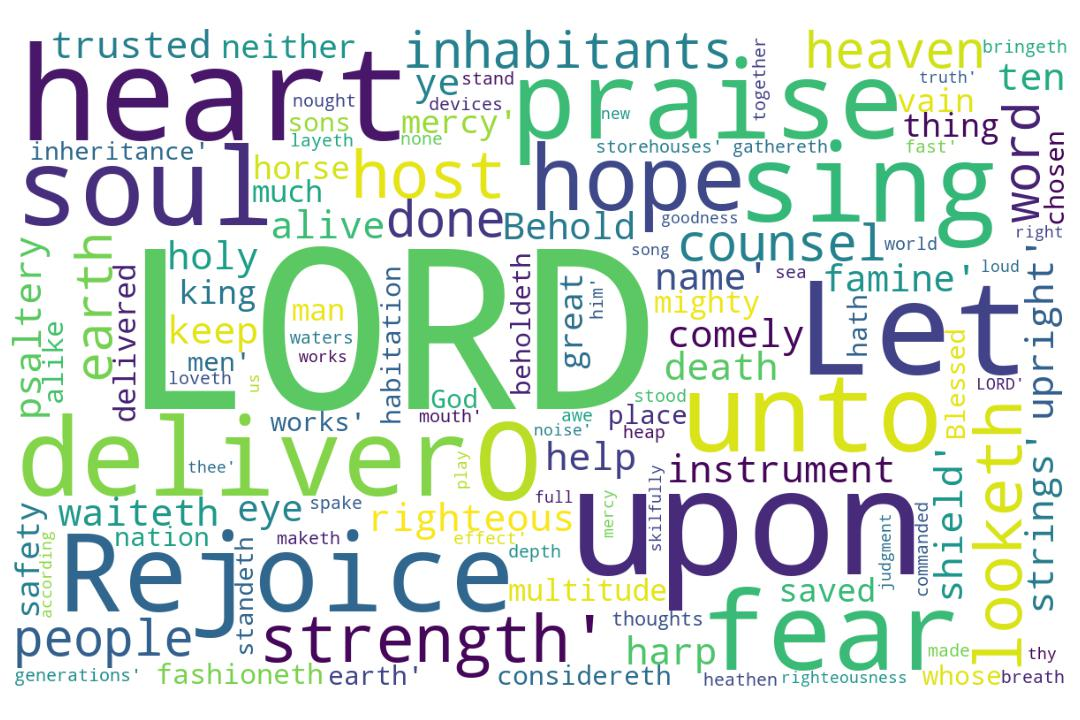
\includegraphics[width=\linewidth]{19OT-Psalms/Psalm33-WordCloud.jpg}
  \caption{Psalm 33 Word Cloud}
  \label{fig:Psalm 33 word Cloud}
\end{figure}

\marginpar{\scriptsize \centering \textbf{\fcolorbox{bone}{lime}{WORSHIP EVERYWHERE}}\\ (Psalm 33:1-22) \begin{compactenum}[I.][8]
    \item \textbf{Worship that Transcends} \index[scripture]{Psalm!Psa 33:01}\index[scripture]{Psalm!Psa 33:02}\index[scripture]{Psalm!Psa 33:03}(Psa 33:1, 2, 3) 
    \item The \textbf{Works that are Told} \index[scripture]{Psalm!Psa 33:04}(Psa 33:4) 
    \item The \textbf{Will that Triumphs} \index[scripture]{Psalm!Psa 33:11}(Psa 33:11) 
    \item The \textbf{Watching that is Thorough} \index[scripture]{Psalm!Psa 33:14}(Psa 33:14) 
    \item The \textbf{World in Turmoil} \index[scripture]{Psalm!Psa 33:19}(Psa 33:19) 
    \item The \textbf{Waiting that Trusts} \index[scripture]{Psalm!Psa 33:21}(Psa 33:21) 
\end{compactenum}}


\marginpar{\scriptsize \centering \textbf{\fcolorbox{bone}{yellow}{WHAT WORSHIP LOOKS LIKE}}\\ (Psalm 33:1-22) \begin{compactenum}[I.][8]
    \item It \textbf{Acknowledges} \index[scripture]{Psalm!Psa 33:01}(Psa 33:1) 
    \item It \textbf{Adorns} with Music\index[scripture]{Psalm!Psa 33:03}(Psa 33:3) 
    \item It \textbf{Asks} in prayer
    \item It is in \textbf{Awe} \index[scripture]{Psalm!Psa 33:08}(Psa 33:8) 
    \item It \textbf{Announces} God's Sovereignty \index[scripture]{Psalm!Psa 33:10}(Psa 33:10) 
    \item It has an \textbf{Attitude} of thankfulness \index[scripture]{Psalm!Psa 33:18}(Psa 33:18) 
    \item It \textbf{Anticipates} \index[scripture]{Psalm!Psa 33:20}(Psa 33:20) 
\end{compactenum}}

\footnote{\textcolor[cmyk]{0.99998,1,0,0}{\hyperlink{TOC}{Return to end of Table of Contents.}}}\footnote{\href{https://audiobible.com/bible/}{\textcolor[cmyk]{0.99998,1,0,0}{Psalms Audio}}}\textcolor[cmyk]{0.99998,1,0,0}{\fcolorbox{bone}{lime}{Rejoice} in the LORD, O ye righteous: \emph{for} praise is comely for the upright.}
[2] \textcolor[cmyk]{0.99998,1,0,0}{\fcolorbox{bone}{lime}{Praise} the LORD with harp: sing unto him with the psaltery \emph{and} an instrument of ten strings.}
[3] \textcolor[cmyk]{0.99998,1,0,0}{\fcolorbox{bone}{lime}{Sing} unto him a new song; play skilfully with a loud noise.}
[4] \textcolor[cmyk]{0.99998,1,0,0}{For the word of the LORD \emph{is} right; and all his \fcolorbox{bone}{lime}{works} \emph{are} \emph{done} in truth.}
[5] \textcolor[cmyk]{0.99998,1,0,0}{He loveth righteousness and judgment: the earth is full of the goodness of the LORD.}
[6] \textcolor[cmyk]{0.99998,1,0,0}{By the word of the LORD were the heavens made; and all the host of them by the breath of his mouth.}
[7] \textcolor[cmyk]{0.99998,1,0,0}{He gathereth the waters of the sea together as an heap: he layeth up the depth in storehouses.}
[8] \textcolor[cmyk]{0.99998,1,0,0}{Let all the earth fear the LORD: let all the inhabitants of the world stand in awe of him.}
[9] \textcolor[cmyk]{0.99998,1,0,0}{For he spake, and it was \emph{done}; he commanded, and it stood fast.}
[10] \textcolor[cmyk]{0.99998,1,0,0}{The LORD bringeth the counsel of the heathen to nought: he maketh the devices of the people of none effect.}
[11] \textcolor[cmyk]{0.99998,1,0,0}{The \fcolorbox{bone}{lime}{counsel} of the LORD standeth for ever, the thoughts of his heart to all generations.}
[12] \textcolor[cmyk]{0.99998,1,0,0}{Blessed \emph{is} the nation whose God \emph{is} the LORD; \emph{and} the people \emph{whom} he hath chosen for his own inheritance.}
[13] \textcolor[cmyk]{0.99998,1,0,0}{The LORD looketh from heaven; he beholdeth all the sons of men.}
[14] \textcolor[cmyk]{0.99998,1,0,0}{From the place of his habitation he \fcolorbox{bone}{lime}{looketh} upon all the inhabitants of the earth.}
[15] \textcolor[cmyk]{0.99998,1,0,0}{He fashioneth their hearts alike; he considereth all their works.}
[16] \textcolor[cmyk]{0.99998,1,0,0}{There is no king saved by the multitude of an host: a mighty man is not delivered by much strength.}
[17] \textcolor[cmyk]{0.99998,1,0,0}{An horse \emph{is} a vain thing for safety: neither shall he deliver \emph{any} by his great strength.}
[18] \textcolor[cmyk]{0.99998,1,0,0}{Behold, the eye of the LORD \emph{is} upon them that fear him, upon them that hope in his mercy;}
[19] \textcolor[cmyk]{0.99998,1,0,0}{To deliver their soul from \fcolorbox{bone}{lime}{death}, and to keep them alive in \fcolorbox{bone}{lime}{famine}.}
[20] \textcolor[cmyk]{0.99998,1,0,0}{Our soul waiteth for the LORD: he \emph{is} our help and our shield.}
[21] \textcolor[cmyk]{0.99998,1,0,0}{For our heart shall rejoice in him, because we have \fcolorbox{bone}{lime}{trusted} in his holy name.}
[22] \textcolor[cmyk]{0.99998,1,0,0}{Let thy mercy, O LORD, be upon us, according as we hope in thee.}
\section{Psalm 33 Comments}

\subsection{Numeric Nuggets}
\textbf{13: } Verses 9, 19, and 20 have 13 words. Verses 1 and 19 have 1 unique words. The word ``LORD'' is found 13 times in the chapter.
%\index[NWIV]{14!Psalms!Psa 33:1}\index[AWIP]{Rejoice!Psalms!Psa 33:1}\index[AWIP]{in!Psalms!Psa 33:1}\index[AWIP]{the!Psalms!Psa 33:1}\index[AWIP]{the!Psalms!Psa 33:1 (2)}\index[AWIP]{LORD!Psalms!Psa 33:1}\index[AWIP]{O!Psalms!Psa 33:1}\index[AWIP]{ye!Psalms!Psa 33:1}\index[AWIP]{righteous!Psalms!Psa 33:1}\index[AWIP]{\emph{for}!Psalms!Psa 33:1}\index[AWIP]{praise!Psalms!Psa 33:1}\index[AWIP]{is!Psalms!Psa 33:1}\index[AWIP]{comely!Psalms!Psa 33:1}\index[AWIP]{for!Psalms!Psa 33:1}\index[AWIP]{upright!Psalms!Psa 33:1}\index[AWIP]{\emph{for}!Psalms!Psa 33:1}

\index[NWIV]{17!Psalms!Psa 33:2}\index[AWIP]{Praise!Psalms!Psa 33:2}\index[AWIP]{the!Psalms!Psa 33:2}\index[AWIP]{the!Psalms!Psa 33:2 (2)}\index[AWIP]{LORD!Psalms!Psa 33:2}\index[AWIP]{with!Psalms!Psa 33:2}\index[AWIP]{with!Psalms!Psa 33:2 (2)}\index[AWIP]{harp!Psalms!Psa 33:2}\index[AWIP]{sing!Psalms!Psa 33:2}\index[AWIP]{unto!Psalms!Psa 33:2}\index[AWIP]{him!Psalms!Psa 33:2}\index[AWIP]{psaltery!Psalms!Psa 33:2}\index[AWIP]{\emph{and}!Psalms!Psa 33:2}\index[AWIP]{an!Psalms!Psa 33:2}\index[AWIP]{instrument!Psalms!Psa 33:2}\index[AWIP]{of!Psalms!Psa 33:2}\index[AWIP]{ten!Psalms!Psa 33:2}\index[AWIP]{strings!Psalms!Psa 33:2}\index[AWIP]{\emph{and}!Psalms!Psa 33:2}

\index[NWIV]{12!Psalms!Psa 33:3}\index[AWIP]{Sing!Psalms!Psa 33:3}\index[AWIP]{unto!Psalms!Psa 33:3}\index[AWIP]{him!Psalms!Psa 33:3}\index[AWIP]{a!Psalms!Psa 33:3}\index[AWIP]{a!Psalms!Psa 33:3 (2)}\index[AWIP]{new!Psalms!Psa 33:3}\index[AWIP]{song!Psalms!Psa 33:3}\index[AWIP]{play!Psalms!Psa 33:3}\index[AWIP]{skilfully!Psalms!Psa 33:3}\index[AWIP]{with!Psalms!Psa 33:3}\index[AWIP]{loud!Psalms!Psa 33:3}\index[AWIP]{noise!Psalms!Psa 33:3}

\index[NWIV]{16!Psalms!Psa 33:4}\index[AWIP]{For!Psalms!Psa 33:4}\index[AWIP]{the!Psalms!Psa 33:4}\index[AWIP]{the!Psalms!Psa 33:4 (2)}\index[AWIP]{word!Psalms!Psa 33:4}\index[AWIP]{of!Psalms!Psa 33:4}\index[AWIP]{LORD!Psalms!Psa 33:4}\index[AWIP]{\emph{is}!Psalms!Psa 33:4}\index[AWIP]{right!Psalms!Psa 33:4}\index[AWIP]{and!Psalms!Psa 33:4}\index[AWIP]{all!Psalms!Psa 33:4}\index[AWIP]{his!Psalms!Psa 33:4}\index[AWIP]{works!Psalms!Psa 33:4}\index[AWIP]{\emph{are}!Psalms!Psa 33:4}\index[AWIP]{\emph{done}!Psalms!Psa 33:4}\index[AWIP]{in!Psalms!Psa 33:4}\index[AWIP]{truth!Psalms!Psa 33:4}\index[AWIP]{\emph{is}!Psalms!Psa 33:4}\index[AWIP]{\emph{are}!Psalms!Psa 33:4}\index[AWIP]{\emph{done}!Psalms!Psa 33:4}

\index[NWIV]{15!Psalms!Psa 33:5}\index[AWIP]{He!Psalms!Psa 33:5}\index[AWIP]{loveth!Psalms!Psa 33:5}\index[AWIP]{righteousness!Psalms!Psa 33:5}\index[AWIP]{and!Psalms!Psa 33:5}\index[AWIP]{judgment!Psalms!Psa 33:5}\index[AWIP]{the!Psalms!Psa 33:5}\index[AWIP]{the!Psalms!Psa 33:5 (2)}\index[AWIP]{the!Psalms!Psa 33:5 (3)}\index[AWIP]{earth!Psalms!Psa 33:5}\index[AWIP]{is!Psalms!Psa 33:5}\index[AWIP]{full!Psalms!Psa 33:5}\index[AWIP]{of!Psalms!Psa 33:5}\index[AWIP]{of!Psalms!Psa 33:5 (2)}\index[AWIP]{goodness!Psalms!Psa 33:5}\index[AWIP]{LORD!Psalms!Psa 33:5}

\index[NWIV]{22!Psalms!Psa 33:6}\index[AWIP]{By!Psalms!Psa 33:6}\index[AWIP]{the!Psalms!Psa 33:6}\index[AWIP]{the!Psalms!Psa 33:6 (2)}\index[AWIP]{the!Psalms!Psa 33:6 (3)}\index[AWIP]{the!Psalms!Psa 33:6 (4)}\index[AWIP]{the!Psalms!Psa 33:6 (5)}\index[AWIP]{word!Psalms!Psa 33:6}\index[AWIP]{of!Psalms!Psa 33:6}\index[AWIP]{of!Psalms!Psa 33:6 (2)}\index[AWIP]{of!Psalms!Psa 33:6 (3)}\index[AWIP]{LORD!Psalms!Psa 33:6}\index[AWIP]{were!Psalms!Psa 33:6}\index[AWIP]{heavens!Psalms!Psa 33:6}\index[AWIP]{made!Psalms!Psa 33:6}\index[AWIP]{and!Psalms!Psa 33:6}\index[AWIP]{all!Psalms!Psa 33:6}\index[AWIP]{host!Psalms!Psa 33:6}\index[AWIP]{them!Psalms!Psa 33:6}\index[AWIP]{by!Psalms!Psa 33:6}\index[AWIP]{breath!Psalms!Psa 33:6}\index[AWIP]{his!Psalms!Psa 33:6}\index[AWIP]{mouth!Psalms!Psa 33:6}

\index[NWIV]{18!Psalms!Psa 33:7}\index[AWIP]{He!Psalms!Psa 33:7}\index[AWIP]{gathereth!Psalms!Psa 33:7}\index[AWIP]{the!Psalms!Psa 33:7}\index[AWIP]{the!Psalms!Psa 33:7 (2)}\index[AWIP]{the!Psalms!Psa 33:7 (3)}\index[AWIP]{waters!Psalms!Psa 33:7}\index[AWIP]{of!Psalms!Psa 33:7}\index[AWIP]{sea!Psalms!Psa 33:7}\index[AWIP]{together!Psalms!Psa 33:7}\index[AWIP]{as!Psalms!Psa 33:7}\index[AWIP]{an!Psalms!Psa 33:7}\index[AWIP]{heap!Psalms!Psa 33:7}\index[AWIP]{he!Psalms!Psa 33:7}\index[AWIP]{layeth!Psalms!Psa 33:7}\index[AWIP]{up!Psalms!Psa 33:7}\index[AWIP]{depth!Psalms!Psa 33:7}\index[AWIP]{in!Psalms!Psa 33:7}\index[AWIP]{storehouses!Psalms!Psa 33:7}

\index[NWIV]{19!Psalms!Psa 33:8}\index[AWIP]{Let!Psalms!Psa 33:8}\index[AWIP]{all!Psalms!Psa 33:8}\index[AWIP]{all!Psalms!Psa 33:8 (2)}\index[AWIP]{the!Psalms!Psa 33:8}\index[AWIP]{the!Psalms!Psa 33:8 (2)}\index[AWIP]{the!Psalms!Psa 33:8 (3)}\index[AWIP]{the!Psalms!Psa 33:8 (4)}\index[AWIP]{earth!Psalms!Psa 33:8}\index[AWIP]{fear!Psalms!Psa 33:8}\index[AWIP]{LORD!Psalms!Psa 33:8}\index[AWIP]{let!Psalms!Psa 33:8}\index[AWIP]{inhabitants!Psalms!Psa 33:8}\index[AWIP]{of!Psalms!Psa 33:8}\index[AWIP]{of!Psalms!Psa 33:8 (2)}\index[AWIP]{world!Psalms!Psa 33:8}\index[AWIP]{stand!Psalms!Psa 33:8}\index[AWIP]{in!Psalms!Psa 33:8}\index[AWIP]{awe!Psalms!Psa 33:8}\index[AWIP]{him!Psalms!Psa 33:8}

\index[NWIV]{13!Psalms!Psa 33:9}\index[AWIP]{For!Psalms!Psa 33:9}\index[AWIP]{he!Psalms!Psa 33:9}\index[AWIP]{he!Psalms!Psa 33:9 (2)}\index[AWIP]{spake!Psalms!Psa 33:9}\index[AWIP]{and!Psalms!Psa 33:9}\index[AWIP]{and!Psalms!Psa 33:9 (2)}\index[AWIP]{it!Psalms!Psa 33:9}\index[AWIP]{it!Psalms!Psa 33:9 (2)}\index[AWIP]{was!Psalms!Psa 33:9}\index[AWIP]{\emph{done}!Psalms!Psa 33:9}\index[AWIP]{commanded!Psalms!Psa 33:9}\index[AWIP]{stood!Psalms!Psa 33:9}\index[AWIP]{fast!Psalms!Psa 33:9}\index[AWIP]{\emph{done}!Psalms!Psa 33:9}

\index[NWIV]{20!Psalms!Psa 33:10}\index[AWIP]{The!Psalms!Psa 33:10}\index[AWIP]{LORD!Psalms!Psa 33:10}\index[AWIP]{bringeth!Psalms!Psa 33:10}\index[AWIP]{the!Psalms!Psa 33:10}\index[AWIP]{the!Psalms!Psa 33:10 (2)}\index[AWIP]{the!Psalms!Psa 33:10 (3)}\index[AWIP]{the!Psalms!Psa 33:10 (4)}\index[AWIP]{counsel!Psalms!Psa 33:10}\index[AWIP]{of!Psalms!Psa 33:10}\index[AWIP]{of!Psalms!Psa 33:10 (2)}\index[AWIP]{of!Psalms!Psa 33:10 (3)}\index[AWIP]{heathen!Psalms!Psa 33:10}\index[AWIP]{to!Psalms!Psa 33:10}\index[AWIP]{nought!Psalms!Psa 33:10}\index[AWIP]{he!Psalms!Psa 33:10}\index[AWIP]{maketh!Psalms!Psa 33:10}\index[AWIP]{devices!Psalms!Psa 33:10}\index[AWIP]{people!Psalms!Psa 33:10}\index[AWIP]{none!Psalms!Psa 33:10}\index[AWIP]{effect!Psalms!Psa 33:10}

\index[NWIV]{16!Psalms!Psa 33:11}\index[AWIP]{The!Psalms!Psa 33:11}\index[AWIP]{counsel!Psalms!Psa 33:11}\index[AWIP]{of!Psalms!Psa 33:11}\index[AWIP]{of!Psalms!Psa 33:11 (2)}\index[AWIP]{the!Psalms!Psa 33:11}\index[AWIP]{the!Psalms!Psa 33:11 (2)}\index[AWIP]{LORD!Psalms!Psa 33:11}\index[AWIP]{standeth!Psalms!Psa 33:11}\index[AWIP]{for!Psalms!Psa 33:11}\index[AWIP]{ever!Psalms!Psa 33:11}\index[AWIP]{thoughts!Psalms!Psa 33:11}\index[AWIP]{his!Psalms!Psa 33:11}\index[AWIP]{heart!Psalms!Psa 33:11}\index[AWIP]{to!Psalms!Psa 33:11}\index[AWIP]{all!Psalms!Psa 33:11}\index[AWIP]{generations!Psalms!Psa 33:11}

\index[NWIV]{20!Psalms!Psa 33:12}\index[AWIP]{Blessed!Psalms!Psa 33:12}\index[AWIP]{\emph{is}!Psalms!Psa 33:12}\index[AWIP]{\emph{is}!Psalms!Psa 33:12 (2)}\index[AWIP]{the!Psalms!Psa 33:12}\index[AWIP]{the!Psalms!Psa 33:12 (2)}\index[AWIP]{the!Psalms!Psa 33:12 (3)}\index[AWIP]{nation!Psalms!Psa 33:12}\index[AWIP]{whose!Psalms!Psa 33:12}\index[AWIP]{God!Psalms!Psa 33:12}\index[AWIP]{LORD!Psalms!Psa 33:12}\index[AWIP]{\emph{and}!Psalms!Psa 33:12}\index[AWIP]{people!Psalms!Psa 33:12}\index[AWIP]{\emph{whom}!Psalms!Psa 33:12}\index[AWIP]{he!Psalms!Psa 33:12}\index[AWIP]{hath!Psalms!Psa 33:12}\index[AWIP]{chosen!Psalms!Psa 33:12}\index[AWIP]{for!Psalms!Psa 33:12}\index[AWIP]{his!Psalms!Psa 33:12}\index[AWIP]{own!Psalms!Psa 33:12}\index[AWIP]{inheritance!Psalms!Psa 33:12}\index[AWIP]{\emph{is}!Psalms!Psa 33:12}\index[AWIP]{\emph{is}!Psalms!Psa 33:12 (2)}\index[AWIP]{\emph{and}!Psalms!Psa 33:12}\index[AWIP]{\emph{whom}!Psalms!Psa 33:12}

\index[NWIV]{12!Psalms!Psa 33:13}\index[AWIP]{The!Psalms!Psa 33:13}\index[AWIP]{LORD!Psalms!Psa 33:13}\index[AWIP]{looketh!Psalms!Psa 33:13}\index[AWIP]{from!Psalms!Psa 33:13}\index[AWIP]{heaven!Psalms!Psa 33:13}\index[AWIP]{he!Psalms!Psa 33:13}\index[AWIP]{beholdeth!Psalms!Psa 33:13}\index[AWIP]{all!Psalms!Psa 33:13}\index[AWIP]{the!Psalms!Psa 33:13}\index[AWIP]{sons!Psalms!Psa 33:13}\index[AWIP]{of!Psalms!Psa 33:13}\index[AWIP]{men!Psalms!Psa 33:13}

\index[NWIV]{15!Psalms!Psa 33:14}\index[AWIP]{From!Psalms!Psa 33:14}\index[AWIP]{the!Psalms!Psa 33:14}\index[AWIP]{the!Psalms!Psa 33:14 (2)}\index[AWIP]{the!Psalms!Psa 33:14 (3)}\index[AWIP]{place!Psalms!Psa 33:14}\index[AWIP]{of!Psalms!Psa 33:14}\index[AWIP]{of!Psalms!Psa 33:14 (2)}\index[AWIP]{his!Psalms!Psa 33:14}\index[AWIP]{habitation!Psalms!Psa 33:14}\index[AWIP]{he!Psalms!Psa 33:14}\index[AWIP]{looketh!Psalms!Psa 33:14}\index[AWIP]{upon!Psalms!Psa 33:14}\index[AWIP]{all!Psalms!Psa 33:14}\index[AWIP]{inhabitants!Psalms!Psa 33:14}\index[AWIP]{earth!Psalms!Psa 33:14}

\index[NWIV]{10!Psalms!Psa 33:15}\index[AWIP]{He!Psalms!Psa 33:15}\index[AWIP]{fashioneth!Psalms!Psa 33:15}\index[AWIP]{their!Psalms!Psa 33:15}\index[AWIP]{their!Psalms!Psa 33:15 (2)}\index[AWIP]{hearts!Psalms!Psa 33:15}\index[AWIP]{alike!Psalms!Psa 33:15}\index[AWIP]{he!Psalms!Psa 33:15}\index[AWIP]{considereth!Psalms!Psa 33:15}\index[AWIP]{all!Psalms!Psa 33:15}\index[AWIP]{works!Psalms!Psa 33:15}

\index[NWIV]{20!Psalms!Psa 33:16}\index[AWIP]{There!Psalms!Psa 33:16}\index[AWIP]{is!Psalms!Psa 33:16}\index[AWIP]{is!Psalms!Psa 33:16 (2)}\index[AWIP]{no!Psalms!Psa 33:16}\index[AWIP]{king!Psalms!Psa 33:16}\index[AWIP]{saved!Psalms!Psa 33:16}\index[AWIP]{by!Psalms!Psa 33:16}\index[AWIP]{by!Psalms!Psa 33:16 (2)}\index[AWIP]{the!Psalms!Psa 33:16}\index[AWIP]{multitude!Psalms!Psa 33:16}\index[AWIP]{of!Psalms!Psa 33:16}\index[AWIP]{an!Psalms!Psa 33:16}\index[AWIP]{host!Psalms!Psa 33:16}\index[AWIP]{a!Psalms!Psa 33:16}\index[AWIP]{mighty!Psalms!Psa 33:16}\index[AWIP]{man!Psalms!Psa 33:16}\index[AWIP]{not!Psalms!Psa 33:16}\index[AWIP]{delivered!Psalms!Psa 33:16}\index[AWIP]{much!Psalms!Psa 33:16}\index[AWIP]{strength!Psalms!Psa 33:16}

\index[NWIV]{17!Psalms!Psa 33:17}\index[AWIP]{An!Psalms!Psa 33:17}\index[AWIP]{horse!Psalms!Psa 33:17}\index[AWIP]{\emph{is}!Psalms!Psa 33:17}\index[AWIP]{a!Psalms!Psa 33:17}\index[AWIP]{vain!Psalms!Psa 33:17}\index[AWIP]{thing!Psalms!Psa 33:17}\index[AWIP]{for!Psalms!Psa 33:17}\index[AWIP]{safety!Psalms!Psa 33:17}\index[AWIP]{neither!Psalms!Psa 33:17}\index[AWIP]{shall!Psalms!Psa 33:17}\index[AWIP]{he!Psalms!Psa 33:17}\index[AWIP]{deliver!Psalms!Psa 33:17}\index[AWIP]{\emph{any}!Psalms!Psa 33:17}\index[AWIP]{by!Psalms!Psa 33:17}\index[AWIP]{his!Psalms!Psa 33:17}\index[AWIP]{great!Psalms!Psa 33:17}\index[AWIP]{strength!Psalms!Psa 33:17}\index[AWIP]{\emph{is}!Psalms!Psa 33:17}\index[AWIP]{\emph{any}!Psalms!Psa 33:17}

\index[NWIV]{19!Psalms!Psa 33:18}\index[AWIP]{Behold!Psalms!Psa 33:18}\index[AWIP]{the!Psalms!Psa 33:18}\index[AWIP]{the!Psalms!Psa 33:18 (2)}\index[AWIP]{eye!Psalms!Psa 33:18}\index[AWIP]{of!Psalms!Psa 33:18}\index[AWIP]{LORD!Psalms!Psa 33:18}\index[AWIP]{\emph{is}!Psalms!Psa 33:18}\index[AWIP]{upon!Psalms!Psa 33:18}\index[AWIP]{upon!Psalms!Psa 33:18 (2)}\index[AWIP]{them!Psalms!Psa 33:18}\index[AWIP]{them!Psalms!Psa 33:18 (2)}\index[AWIP]{that!Psalms!Psa 33:18}\index[AWIP]{that!Psalms!Psa 33:18 (2)}\index[AWIP]{fear!Psalms!Psa 33:18}\index[AWIP]{him!Psalms!Psa 33:18}\index[AWIP]{hope!Psalms!Psa 33:18}\index[AWIP]{in!Psalms!Psa 33:18}\index[AWIP]{his!Psalms!Psa 33:18}\index[AWIP]{mercy!Psalms!Psa 33:18}\index[AWIP]{\emph{is}!Psalms!Psa 33:18}

\index[NWIV]{13!Psalms!Psa 33:19}\index[AWIP]{To!Psalms!Psa 33:19}\index[AWIP]{deliver!Psalms!Psa 33:19}\index[AWIP]{their!Psalms!Psa 33:19}\index[AWIP]{soul!Psalms!Psa 33:19}\index[AWIP]{from!Psalms!Psa 33:19}\index[AWIP]{death!Psalms!Psa 33:19}\index[AWIP]{and!Psalms!Psa 33:19}\index[AWIP]{to!Psalms!Psa 33:19}\index[AWIP]{keep!Psalms!Psa 33:19}\index[AWIP]{them!Psalms!Psa 33:19}\index[AWIP]{alive!Psalms!Psa 33:19}\index[AWIP]{in!Psalms!Psa 33:19}\index[AWIP]{famine!Psalms!Psa 33:19}

\index[NWIV]{13!Psalms!Psa 33:20}\index[AWIP]{Our!Psalms!Psa 33:20}\index[AWIP]{soul!Psalms!Psa 33:20}\index[AWIP]{waiteth!Psalms!Psa 33:20}\index[AWIP]{for!Psalms!Psa 33:20}\index[AWIP]{the!Psalms!Psa 33:20}\index[AWIP]{LORD!Psalms!Psa 33:20}\index[AWIP]{he!Psalms!Psa 33:20}\index[AWIP]{\emph{is}!Psalms!Psa 33:20}\index[AWIP]{our!Psalms!Psa 33:20}\index[AWIP]{our!Psalms!Psa 33:20 (2)}\index[AWIP]{help!Psalms!Psa 33:20}\index[AWIP]{and!Psalms!Psa 33:20}\index[AWIP]{shield!Psalms!Psa 33:20}\index[AWIP]{\emph{is}!Psalms!Psa 33:20}

\index[NWIV]{15!Psalms!Psa 33:21}\index[AWIP]{For!Psalms!Psa 33:21}\index[AWIP]{our!Psalms!Psa 33:21}\index[AWIP]{heart!Psalms!Psa 33:21}\index[AWIP]{shall!Psalms!Psa 33:21}\index[AWIP]{rejoice!Psalms!Psa 33:21}\index[AWIP]{in!Psalms!Psa 33:21}\index[AWIP]{in!Psalms!Psa 33:21 (2)}\index[AWIP]{him!Psalms!Psa 33:21}\index[AWIP]{because!Psalms!Psa 33:21}\index[AWIP]{we!Psalms!Psa 33:21}\index[AWIP]{have!Psalms!Psa 33:21}\index[AWIP]{trusted!Psalms!Psa 33:21}\index[AWIP]{his!Psalms!Psa 33:21}\index[AWIP]{holy!Psalms!Psa 33:21}\index[AWIP]{name!Psalms!Psa 33:21}

\index[NWIV]{14!Psalms!Psa 33:22}\index[AWIP]{Let!Psalms!Psa 33:22}\index[AWIP]{thy!Psalms!Psa 33:22}\index[AWIP]{mercy!Psalms!Psa 33:22}\index[AWIP]{O!Psalms!Psa 33:22}\index[AWIP]{LORD!Psalms!Psa 33:22}\index[AWIP]{be!Psalms!Psa 33:22}\index[AWIP]{upon!Psalms!Psa 33:22}\index[AWIP]{us!Psalms!Psa 33:22}\index[AWIP]{according!Psalms!Psa 33:22}\index[AWIP]{as!Psalms!Psa 33:22}\index[AWIP]{we!Psalms!Psa 33:22}\index[AWIP]{hope!Psalms!Psa 33:22}\index[AWIP]{in!Psalms!Psa 33:22}\index[AWIP]{thee!Psalms!Psa 33:22}


\section{Psalm 33 Outlines}

\subsection{My Outlines}

\subsubsection{Worship Everywhere}
\index[speaker]{Keith Anthony!Psalm 033 (Worship Everywhere)}
\index[series]{Psalms (Keith Anthony)!Psalm 033 (Worship Everywhere)}
\index[date]{2010/02/01!Psalm 033 (Worship Everywhere) (Keith Anthony)}
\begin{compactenum}[I.]
    \item \textbf{Worship that Transcends} \index[scripture]{Psalm!Psa 33:01}\index[scripture]{Psalm!Psa 33:02}\index[scripture]{Psalm!Psa 33:03}(Psa 33:1, 2, 3) 
    \item The \textbf{Works that are Told} \index[scripture]{Psalm!Psa 33:04}(Psa 33:4) 
    \item The \textbf{Will that Triumphs} \index[scripture]{Psalm!Psa 33:11}(Psa 33:11) 
    \item The \textbf{Watching that is Thorough} \index[scripture]{Psalm!Psa 33:14}(Psa 33:14) 
    \item The \textbf{World in Turmoil} \index[scripture]{Psalm!Psa 33:19}(Psa 33:19) 
    \item The \textbf{Waiting that Trusts} \index[scripture]{Psalm!Psa 33:21}(Psa 33:21) 
\end{compactenum}

\subsubsection{What Worship Looks Like}
\index[speaker]{Keith Anthony!Psalm 033 (What Worship Looks Like)}
\index[series]{Psalms (Keith Anthony)!Psalm 033 (What Worship Looks Like}
\index[date]{2019/02/02!Psalm 033 (What Worship Looks Like (Keith Anthony)}
\begin{compactenum}[I.][8]
    \item It \textbf{Acknowledges} \index[scripture]{Psalm!Psa 33:01}(Psa 33:1) 
    \item It \textbf{Adorns} with Music\index[scripture]{Psalm!Psa 33:03}(Psa 33:3) 
    \item It \textbf{Asks} in prayer
    \item It is in \textbf{Awe} \index[scripture]{Psalm!Psa 33:08}(Psa 33:8) 
    \item It \textbf{Announces} God's Sovereignty \index[scripture]{Psalm!Psa 33:10}(Psa 33:10) 
    \item It has an \textbf{Attitude} of thankfulness \index[scripture]{Psalm!Psa 33:18}(Psa 33:18) 
    \item It \textbf{Anticipates} \index[scripture]{Psalm!Psa 33:20}(Psa 33:20) 
\end{compactenum}
\subsection{Outlines from Others}

\subsubsection{One Focus}
\index[speaker]{Ricky Bell!Psalm 033:12 (One Focus)}
\index[series]{Psalms (Ricky Bell)!Psalm 033:12 (One Focus)}
\index[date]{2011/09/11!Psalm 033:12 (One Focus) (Ricky Bell)}
\textbf{Creator: } Ricky Bell
\begin{compactenum}[I.]
		\item One Goal
		\item One Book
		\item One People
		\item One King
%    \item \textbf{Confirmation of Forgiveness} \index[scripture]{Psalms!Psalm 032:01-02}(Psalm 32:1-2)
%    \item \textbf{Confession of Sin} \index[scripture]{Psalms!Psalm 032:03-05}(Psalm 32:3-5)
%    \item \textbf{Counsel to a Saint} \index[scripture]{Psalms!Psalm 032:06}(Psalm 32:6)
%    \item \textbf{Contentment in the Lord} \index[scripture]{Psalms!Psalm 032:07-11}(Psalm 32:7-11)
%    \item \textbf{Correction to the Walk} \index[scripture]{Psalms!Psalm 032:09}(Psalm 32:9)
%    \item \textbf{Conclusion to the Matter} \index[scripture]{Psalms!Psalm 032:10-11}(Psalm 32:10-11)
\end{compactenum}


%\section{Psalm 33 Statistics}

%%%%%%%%%%%%%%%%%%%%%%%%%%%
%%%%% Word Statistics
%%%%%%%%%%%%%%%%%%%%%%%%%%


\normalsize



\subsection{Chapter Word Statistics}


%%%%%%%%%%
%%%%%%%%%%
 
\begin{center}
\begin{longtable}{l|c|c|c|c}
\caption[Stats for Psalm 33]{Stats for Psalm 33} \label{table:Stats for Psalm 33} \\ 
\hline \multicolumn{1}{|c|}{\textbf{Verse(s)}} & \multicolumn{1}{|c|}{\textbf{Count}} & \multicolumn{1}{|c|}{\textbf{Unique}} & \multicolumn{1}{|c|}{\textbf{Italics}} & \multicolumn{1}{|c|}{\textbf{Uniq Italic}}  \\ \hline 
\endfirsthead
 
\multicolumn{5}{c}
{{\bfseries \tablename\ \thetable{} -- continued from previous page}} \\  
\hline \multicolumn{1}{|c|}{\textbf{Verse(s)}} & \multicolumn{1}{|c|}{\textbf{Count}} & \multicolumn{1}{|c|}{\textbf{Unique}} & \multicolumn{1}{|c|}{\textbf{Italics}} & \multicolumn{1}{|c|}{\textbf{Uniq Italic}}  \\ \hline 
\endhead
 
\hline \multicolumn{5}{|r|}{{Continued if needed}} \\ \hline
\endfoot 
1 & 14 & 13 & 1 & 1\\ \hline
2 & 17 & 15 & 1 & 1\\ \hline
3 & 12 & 11 & 0 & 0\\ \hline
4 & 16 & 15 & 3 & 3\\ \hline
5 & 15 & 12 & 0 & 0\\ \hline
6 & 22 & 16 & 0 & 0\\ \hline
7 & 18 & 16 & 0 & 0\\ \hline
8 & 19 & 14 & 0 & 0\\ \hline
9 & 13 & 10 & 1 & 1\\ \hline
10 & 20 & 15 & 0 & 0\\ \hline
11 & 16 & 14 & 0 & 0\\ \hline
12 & 20 & 17 & 4 & 3\\ \hline
13 & 12 & 12 & 0 & 0\\ \hline
14 & 15 & 12 & 0 & 0\\ \hline
15 & 10 & 9 & 0 & 0\\ \hline
16 & 20 & 18 & 0 & 0\\ \hline
17 & 17 & 17 & 2 & 2\\ \hline
18 & 19 & 15 & 1 & 1\\ \hline
19 & 13 & 13 & 0 & 0\\ \hline
20 & 13 & 12 & 1 & 1\\ \hline
21 & 15 & 14 & 0 & 0\\ \hline
22 & 14 & 14 & 0 & 0\\ \hline
\hline \hline
Total & 350 & 174 & 14 & 7



\end{longtable}
\end{center}

%%%%%%%%%%
%%%%%%%%%%
 
\subsection{Words by Frequency}

\begin{center}
\begin{longtable}{l|r}
\caption[Word Frequencies in Psalm 33]{Word Frequencies in Psalm 33} \label{table:WordsIn-Psalm-33} \\ 
\hline \multicolumn{1}{|c|}{\textbf{Word}} & \multicolumn{1}{c|}{\textbf{Frequency}} \\ \hline 
\endfirsthead
 
\multicolumn{2}{c}
{{\bfseries \tablename\ \thetable{} -- continued from previous page}} \\ 
\hline \multicolumn{1}{|c|}{\textbf{Word}} & \multicolumn{1}{c|}{\textbf{Frequency}} \\ \hline 
\endhead
 
\hline \multicolumn{2}{|r|}{{Continued if needed}} \\ \hline
\endfoot
 
\hline \hline
\endlastfoot
the & 38 \\ \hline
of & 20 \\ \hline
LORD & 13 \\ \hline
he & 10 \\ \hline
in & 9 \\ \hline
all & 8 \\ \hline
his & 8 \\ \hline
and & 7 \\ \hline
\emph{is} & 6 \\ \hline
for & 5 \\ \hline
him & 5 \\ \hline
is & 4 \\ \hline
a & 4 \\ \hline
them & 4 \\ \hline
by & 4 \\ \hline
upon & 4 \\ \hline
with & 3 \\ \hline
an & 3 \\ \hline
For & 3 \\ \hline
He & 3 \\ \hline
earth & 3 \\ \hline
The & 3 \\ \hline
to & 3 \\ \hline
their & 3 \\ \hline
our & 3 \\ \hline
O & 2 \\ \hline
unto & 2 \\ \hline
\emph{and} & 2 \\ \hline
word & 2 \\ \hline
works & 2 \\ \hline
\emph{done} & 2 \\ \hline
host & 2 \\ \hline
as & 2 \\ \hline
Let & 2 \\ \hline
fear & 2 \\ \hline
inhabitants & 2 \\ \hline
it & 2 \\ \hline
counsel & 2 \\ \hline
people & 2 \\ \hline
heart & 2 \\ \hline
looketh & 2 \\ \hline
from & 2 \\ \hline
strength & 2 \\ \hline
shall & 2 \\ \hline
deliver & 2 \\ \hline
that & 2 \\ \hline
hope & 2 \\ \hline
mercy & 2 \\ \hline
soul & 2 \\ \hline
we & 2 \\ \hline
Rejoice & 1 \\ \hline
ye & 1 \\ \hline
righteous & 1 \\ \hline
\emph{for} & 1 \\ \hline
praise & 1 \\ \hline
comely & 1 \\ \hline
upright & 1 \\ \hline
Praise & 1 \\ \hline
harp & 1 \\ \hline
sing & 1 \\ \hline
psaltery & 1 \\ \hline
instrument & 1 \\ \hline
ten & 1 \\ \hline
strings & 1 \\ \hline
Sing & 1 \\ \hline
new & 1 \\ \hline
song & 1 \\ \hline
play & 1 \\ \hline
skilfully & 1 \\ \hline
loud & 1 \\ \hline
noise & 1 \\ \hline
right & 1 \\ \hline
\emph{are} & 1 \\ \hline
truth & 1 \\ \hline
loveth & 1 \\ \hline
righteousness & 1 \\ \hline
judgment & 1 \\ \hline
full & 1 \\ \hline
goodness & 1 \\ \hline
By & 1 \\ \hline
were & 1 \\ \hline
heavens & 1 \\ \hline
made & 1 \\ \hline
breath & 1 \\ \hline
mouth & 1 \\ \hline
gathereth & 1 \\ \hline
waters & 1 \\ \hline
sea & 1 \\ \hline
together & 1 \\ \hline
heap & 1 \\ \hline
layeth & 1 \\ \hline
up & 1 \\ \hline
depth & 1 \\ \hline
storehouses & 1 \\ \hline
let & 1 \\ \hline
world & 1 \\ \hline
stand & 1 \\ \hline
awe & 1 \\ \hline
spake & 1 \\ \hline
was & 1 \\ \hline
commanded & 1 \\ \hline
stood & 1 \\ \hline
fast & 1 \\ \hline
bringeth & 1 \\ \hline
heathen & 1 \\ \hline
nought & 1 \\ \hline
maketh & 1 \\ \hline
devices & 1 \\ \hline
none & 1 \\ \hline
effect & 1 \\ \hline
standeth & 1 \\ \hline
ever & 1 \\ \hline
thoughts & 1 \\ \hline
generations & 1 \\ \hline
Blessed & 1 \\ \hline
nation & 1 \\ \hline
whose & 1 \\ \hline
God & 1 \\ \hline
\emph{whom} & 1 \\ \hline
hath & 1 \\ \hline
chosen & 1 \\ \hline
own & 1 \\ \hline
inheritance & 1 \\ \hline
heaven & 1 \\ \hline
beholdeth & 1 \\ \hline
sons & 1 \\ \hline
men & 1 \\ \hline
From & 1 \\ \hline
place & 1 \\ \hline
habitation & 1 \\ \hline
fashioneth & 1 \\ \hline
hearts & 1 \\ \hline
alike & 1 \\ \hline
considereth & 1 \\ \hline
There & 1 \\ \hline
no & 1 \\ \hline
king & 1 \\ \hline
saved & 1 \\ \hline
multitude & 1 \\ \hline
mighty & 1 \\ \hline
man & 1 \\ \hline
not & 1 \\ \hline
delivered & 1 \\ \hline
much & 1 \\ \hline
An & 1 \\ \hline
horse & 1 \\ \hline
vain & 1 \\ \hline
thing & 1 \\ \hline
safety & 1 \\ \hline
neither & 1 \\ \hline
\emph{any} & 1 \\ \hline
great & 1 \\ \hline
Behold & 1 \\ \hline
eye & 1 \\ \hline
To & 1 \\ \hline
death & 1 \\ \hline
keep & 1 \\ \hline
alive & 1 \\ \hline
famine & 1 \\ \hline
Our & 1 \\ \hline
waiteth & 1 \\ \hline
help & 1 \\ \hline
shield & 1 \\ \hline
rejoice & 1 \\ \hline
because & 1 \\ \hline
have & 1 \\ \hline
trusted & 1 \\ \hline
holy & 1 \\ \hline
name & 1 \\ \hline
thy & 1 \\ \hline
be & 1 \\ \hline
us & 1 \\ \hline
according & 1 \\ \hline
thee & 1 \\ \hline
\end{longtable}
\end{center}



\normalsize



\subsection{Words Alphabetically}

\begin{center}
\begin{longtable}{l|r}
\caption[Word Alphabetically in Psalm 33]{Word Alphabetically in Psalm 33} \label{table:WordsIn-Psalm-33} \\ 
\hline \multicolumn{1}{|c|}{\textbf{Word}} & \multicolumn{1}{c|}{\textbf{Frequency}} \\ \hline 
\endfirsthead
 
\multicolumn{2}{c}
{{\bfseries \tablename\ \thetable{} -- continued from previous page}} \\ 
\hline \multicolumn{1}{|c|}{\textbf{Word}} & \multicolumn{1}{c|}{\textbf{Frequency}} \\ \hline 
\endhead
 
\hline \multicolumn{2}{|r|}{{Continued if needed}} \\ \hline
\endfoot
 
\hline \hline
\endlastfoot
An & 1 \\ \hline
Behold & 1 \\ \hline
Blessed & 1 \\ \hline
By & 1 \\ \hline
For & 3 \\ \hline
From & 1 \\ \hline
God & 1 \\ \hline
He & 3 \\ \hline
LORD & 13 \\ \hline
Let & 2 \\ \hline
O & 2 \\ \hline
Our & 1 \\ \hline
Praise & 1 \\ \hline
Rejoice & 1 \\ \hline
Sing & 1 \\ \hline
The & 3 \\ \hline
There & 1 \\ \hline
To & 1 \\ \hline
\emph{and} & 2 \\ \hline
\emph{any} & 1 \\ \hline
\emph{are} & 1 \\ \hline
\emph{done} & 2 \\ \hline
\emph{for} & 1 \\ \hline
\emph{is} & 6 \\ \hline
\emph{whom} & 1 \\ \hline
a & 4 \\ \hline
according & 1 \\ \hline
alike & 1 \\ \hline
alive & 1 \\ \hline
all & 8 \\ \hline
an & 3 \\ \hline
and & 7 \\ \hline
as & 2 \\ \hline
awe & 1 \\ \hline
be & 1 \\ \hline
because & 1 \\ \hline
beholdeth & 1 \\ \hline
breath & 1 \\ \hline
bringeth & 1 \\ \hline
by & 4 \\ \hline
chosen & 1 \\ \hline
comely & 1 \\ \hline
commanded & 1 \\ \hline
considereth & 1 \\ \hline
counsel & 2 \\ \hline
death & 1 \\ \hline
deliver & 2 \\ \hline
delivered & 1 \\ \hline
depth & 1 \\ \hline
devices & 1 \\ \hline
earth & 3 \\ \hline
effect & 1 \\ \hline
ever & 1 \\ \hline
eye & 1 \\ \hline
famine & 1 \\ \hline
fashioneth & 1 \\ \hline
fast & 1 \\ \hline
fear & 2 \\ \hline
for & 5 \\ \hline
from & 2 \\ \hline
full & 1 \\ \hline
gathereth & 1 \\ \hline
generations & 1 \\ \hline
goodness & 1 \\ \hline
great & 1 \\ \hline
habitation & 1 \\ \hline
harp & 1 \\ \hline
hath & 1 \\ \hline
have & 1 \\ \hline
he & 10 \\ \hline
heap & 1 \\ \hline
heart & 2 \\ \hline
hearts & 1 \\ \hline
heathen & 1 \\ \hline
heaven & 1 \\ \hline
heavens & 1 \\ \hline
help & 1 \\ \hline
him & 5 \\ \hline
his & 8 \\ \hline
holy & 1 \\ \hline
hope & 2 \\ \hline
horse & 1 \\ \hline
host & 2 \\ \hline
in & 9 \\ \hline
inhabitants & 2 \\ \hline
inheritance & 1 \\ \hline
instrument & 1 \\ \hline
is & 4 \\ \hline
it & 2 \\ \hline
judgment & 1 \\ \hline
keep & 1 \\ \hline
king & 1 \\ \hline
layeth & 1 \\ \hline
let & 1 \\ \hline
looketh & 2 \\ \hline
loud & 1 \\ \hline
loveth & 1 \\ \hline
made & 1 \\ \hline
maketh & 1 \\ \hline
man & 1 \\ \hline
men & 1 \\ \hline
mercy & 2 \\ \hline
mighty & 1 \\ \hline
mouth & 1 \\ \hline
much & 1 \\ \hline
multitude & 1 \\ \hline
name & 1 \\ \hline
nation & 1 \\ \hline
neither & 1 \\ \hline
new & 1 \\ \hline
no & 1 \\ \hline
noise & 1 \\ \hline
none & 1 \\ \hline
not & 1 \\ \hline
nought & 1 \\ \hline
of & 20 \\ \hline
our & 3 \\ \hline
own & 1 \\ \hline
people & 2 \\ \hline
place & 1 \\ \hline
play & 1 \\ \hline
praise & 1 \\ \hline
psaltery & 1 \\ \hline
rejoice & 1 \\ \hline
right & 1 \\ \hline
righteous & 1 \\ \hline
righteousness & 1 \\ \hline
safety & 1 \\ \hline
saved & 1 \\ \hline
sea & 1 \\ \hline
shall & 2 \\ \hline
shield & 1 \\ \hline
sing & 1 \\ \hline
skilfully & 1 \\ \hline
song & 1 \\ \hline
sons & 1 \\ \hline
soul & 2 \\ \hline
spake & 1 \\ \hline
stand & 1 \\ \hline
standeth & 1 \\ \hline
stood & 1 \\ \hline
storehouses & 1 \\ \hline
strength & 2 \\ \hline
strings & 1 \\ \hline
ten & 1 \\ \hline
that & 2 \\ \hline
the & 38 \\ \hline
thee & 1 \\ \hline
their & 3 \\ \hline
them & 4 \\ \hline
thing & 1 \\ \hline
thoughts & 1 \\ \hline
thy & 1 \\ \hline
to & 3 \\ \hline
together & 1 \\ \hline
trusted & 1 \\ \hline
truth & 1 \\ \hline
unto & 2 \\ \hline
up & 1 \\ \hline
upon & 4 \\ \hline
upright & 1 \\ \hline
us & 1 \\ \hline
vain & 1 \\ \hline
waiteth & 1 \\ \hline
was & 1 \\ \hline
waters & 1 \\ \hline
we & 2 \\ \hline
were & 1 \\ \hline
whose & 1 \\ \hline
with & 3 \\ \hline
word & 2 \\ \hline
works & 2 \\ \hline
world & 1 \\ \hline
ye & 1 \\ \hline
\end{longtable}
\end{center}



\normalsize



\subsection{Word Lengths in Chapter}
\normalsize
\begin{longtable}{l|p{3.75in}}
\caption[Words by Length in Psalm 33]{Words by Length in Psalm 33} \label{table:WordsIn-Psalm-33} \\ 
\hline \multicolumn{1}{|c|}{\textbf{Length}} & \multicolumn{1}{c|}{\textbf{Words}} \\ \hline 
\endfirsthead
 
\multicolumn{2}{c}
{{\bfseries \tablename\ \thetable{} -- continued from previous page}} \\ 
\hline \multicolumn{1}{|c|}{\textbf{Length}} & \multicolumn{1}{c|}{\textbf{Words}} \\ \hline 
\endhead
 
\hline \multicolumn{2}{|r|}{{Continued if needed}} \\ \hline
\endfoot
 
\hline \hline
\endlastfoot
1 & O, a \\ \hline
2 & in, ye, is, an, of, \emph{is}, He, By, by, as, he, up, it, to, no, An, To, we, be, us \\ \hline
3 & the, \emph{for}, for, him, \emph{and}, ten, new, For, and, all, his, \emph{are}, sea, Let, let, awe, was, The, God, own, men, man, not, \emph{any}, eye, Our, our, thy \\ \hline
4 & LORD, with, harp, sing, unto, Sing, song, play, loud, word, \emph{done}, full, were, made, host, them, heap, fear, fast, none, ever, \emph{whom}, hath, from, sons, From, upon, king, much, vain, that, hope, soul, keep, help, have, holy, name, thee \\ \hline
5 & noise, right, works, truth, earth, mouth, depth, world, stand, spake, stood, heart, whose, place, their, alike, There, saved, horse, thing, shall, great, mercy, death, alive \\ \hline
6 & praise, comely, Praise, loveth, breath, waters, layeth, nought, maketh, people, effect, nation, chosen, heaven, hearts, mighty, safety, Behold, famine, shield \\ \hline
7 & Rejoice, upright, strings, heavens, counsel, heathen, devices, Blessed, looketh, neither, deliver, waiteth, rejoice, because, trusted \\ \hline
8 & psaltery, judgment, goodness, together, bringeth, standeth, thoughts, strength \\ \hline
9 & righteous, skilfully, gathereth, commanded, beholdeth, multitude, delivered, according \\ \hline
10 & instrument, habitation, fashioneth \\ \hline
11 & storehouses, inhabitants, generations, inheritance, considereth \\ \hline
13 & righteousness \\ \hline
\end{longtable}






%%%%%%%%%%
%%%%%%%%%%
 



%%%%%%%%%%
%%%%%%%%%%
\subsection{Verses with 13 Words in Chapter}
\normalsize
\begin{longtable}{l|p{3.75in}}
\caption[Verses with 13 Words  in Psalm 33]{Verses with 13 Words  in Psalm 33} \label{table:Verses with 13 Words in-Psalm-33} \\ 
\hline \multicolumn{1}{|c|}{\textbf{Reference}} & \multicolumn{1}{c|}{\textbf{Verse}} \\ \hline 
\endfirsthead
 
\multicolumn{2}{c}
{{\bfseries \tablename\ \thetable{} -- continued from previous page}} \\ 
\hline \multicolumn{1}{|c|}{\textbf{Reference}} & \multicolumn{1}{c|}{\textbf{Verse}} \\ \hline 
\endhead
 
\hline \multicolumn{2}{|r|}{{Continued if needed}} \\ \hline
\endfoot
 
\hline \hline
\endlastfoot
Psalms 033:9 & For he spake, and it was \emph{done}; he commanded, and it stood fast. \\ \hline
Psalms 033:19 & To deliver their soul from death, and to keep them alive in famine. \\ \hline
Psalms 033:20 & Our soul waiteth for the LORD: he \emph{is} our help and our shield. \\ \hline
\end{longtable}






%%%%%%%%%%
%%%%%%%%%%
 



%%%%%%%%%%
%%%%%%%%%%
\subsection{Verses with 18 Words in Chapter}
\normalsize
\begin{longtable}{l|p{3.75in}}
\caption[Verses with 18 Words  in Psalm 33]{Verses with 18 Words  in Psalm 33} \label{table:Verses with 18 Words in-Psalm-33} \\ 
\hline \multicolumn{1}{|c|}{\textbf{Reference}} & \multicolumn{1}{c|}{\textbf{Verse}} \\ \hline 
\endfirsthead
 
\multicolumn{2}{c}
{{\bfseries \tablename\ \thetable{} -- continued from previous page}} \\ 
\hline \multicolumn{1}{|c|}{\textbf{Reference}} & \multicolumn{1}{c|}{\textbf{Verse}} \\ \hline 
\endhead
 
\hline \multicolumn{2}{|r|}{{Continued if needed}} \\ \hline
\endfoot
 
\hline \hline
\endlastfoot
Psalms 033:7 & He gathereth the waters of the sea together as an heap: he layeth up the depth in storehouses. \\ \hline
\end{longtable}






%%%%%%%%%%
%%%%%%%%%%
\subsection{Psalm 33 Repeated Phrases}


%%%%%%%%%%
%%%%%%%%%%
\normalsize
 
\begin{center}
\begin{longtable}{|p{3.0in}|p{0.5in}|}
\caption[Psalm 33 Repeated Phrases]{Psalm 33 Repeated Phrases}\label{table:Repeated Phrases Psalm 33} \\
\hline \multicolumn{1}{|c|}{\textbf{Phrase}} & \multicolumn{1}{c|}{\textbf{Frequency}} \\ \hline 
\endfirsthead
 
\multicolumn{2}{c}
{{\bfseries \tablename\ \thetable{} -- continued from previous page}} \\  
\hline \multicolumn{1}{|c|}{\textbf{Phrase}} & \multicolumn{1}{c|}{\textbf{Frequency}} \\ \hline 
\endhead
 
\hline \multicolumn{2}{c}{{ }} \\ \hline
\endfoot 
of the & 11\\ \hline 
the LORD & 10\\ \hline 
of the LORD & 5\\ \hline 
all the & 5\\ \hline 
the earth & 3\\ \hline 
of his & 3\\ \hline 
\end{longtable}
\end{center}



%%%%%%%%%%
%%%%%%%%%%




\chapter{Psalm 34}

\begin{figure}
  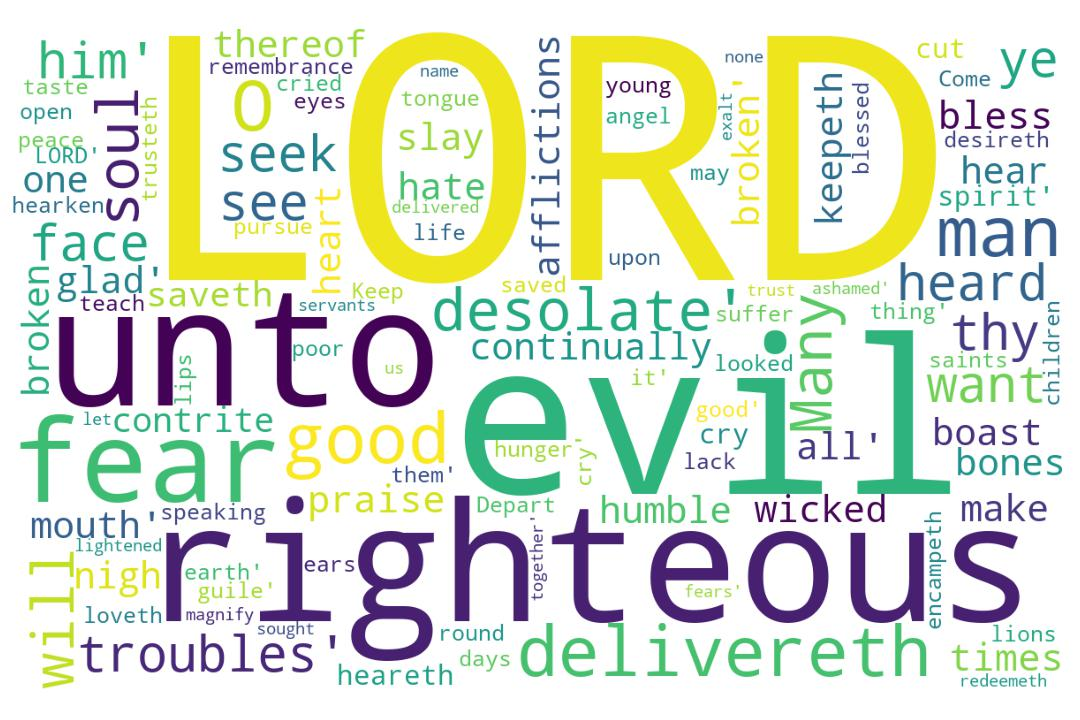
\includegraphics[width=\linewidth]{19OT-Psalms/Psalm34-WordCloud.jpg}
  \caption{Psalm 34 Word Cloud}
  \label{fig:Psalm 34 word Cloud}
\end{figure}


\marginpar{\scriptsize \centering \fcolorbox{bone}{lime}{\textbf{A FAITH WORTH HAVING}}\\ (Psalm 34:1--22) 
\begin{compactenum}[I.][8]
    \item In One I can \textbf{Continually Praise} the Lord \index[scripture]{Psalms!Psa 034:01}(Psa 34:1)
    \item In One that is \textbf{Constantly Present} \index[scripture]{Psalms!Psa 034:01}(Psa 34:1)
    \item In One who \textbf{Considers my Pleas} \index[scripture]{Psalms!Psa 034:06}(Psa 34:6)
    \item In one who is \textbf{Certifiably Proven} \index[scripture]{Psalms!Psa 034:08}(Psa 34:8)
    \item In whom I Get \textbf{Unceasing Provision} \index[scripture]{Psalms!Psa 034:09}(Psa 34:9)
    \item In whom who Provides \textbf{Comforting Proximity} \index[scripture]{Psalms!Psa 034:18}(Psa 34:18)
\end{compactenum} }

\marginpar{\scriptsize \centering \fcolorbox{bone}{yellow}{\textbf{IMPERATIVES FOR THE BELIEVER}}\\ (Psalm 34:1--22) 
\begin{compactenum}[I.][8]
    \item \textbf{Bless} the Lord \index[scripture]{Psalms!Psa 034:01}(Psa 34:1)
    \item \textbf{Praise} the Lord \index[scripture]{Psalms!Psa 034:01}(Psa 34:1)
    \item \textbf{Boast} of the Lord \index[scripture]{Psalms!Psa 034:02}(Psa 34:2)
    \item \textbf{Magnify} the Lord \index[scripture]{Psalms!Psa 034:03}(Psa 34:3)
    \item \textbf{Exalt} the Lord \index[scripture]{Psalms!Psa 034:03}(Psa 34:3)
    \item \textbf{Seek} the Lord \index[scripture]{Psalms!Psa 034:04}(Psa 34:4)
    \item \textbf{Taste} the Lord \index[scripture]{Psalms!Psa 034:08}(Psa 34:8)
    \item \textbf{Trust} in the Lord \index[scripture]{Psalms!Psa 034:08}(Psa 34:8)
\end{compactenum}}

\marginpar{\scriptsize \centering \fcolorbox{bone}{black}{\textbf{\textcolor[cmyk]{0,0,0,0}{AN INVOLVED GOD}}}\\ (Psalm 34) 
\begin{compactenum}[I.][8]
    \item He \textbf{Enlightens} his People \index[scripture]{Psalms!Psa 034:05} (Psa 34:5)
    \item He \textbf{Lingers} Nearby \index[scripture]{Psalms!Psa 034:07}\index[scripture]{Psalms!Psa 034:18} (Psa 34:7, 18)
    \item He is \textbf{Longing} to Bless \index[scripture]{Psalms!Psa 034:10}(Psa 34:10)
    \item He is \textbf{Looking} at the Saints \index[scripture]{Psalms!Psa 034:15}(Psa 34:15)
    \item He is \textbf{Listening} for their Prayers \index[scripture]{Psalms!Psa 034:15}(Psa 34:15)
    \item He is \textbf{Looming} against Evil\index[scripture]{Psalms!Psa 034:16}(Psa 34:16)
\end{compactenum} }

\footnote{\textcolor[cmyk]{0.99998,1,0,0}{\hyperlink{TOC}{Return to end of Table of Contents.}}}\footnote{\href{https://www.audioverse.org/english/audiobibles/books/ENGKJV/O/Ps/1}{\textcolor[cmyk]{0.99998,1,0,0}{Psalms Audio}}}\textcolor[cmyk]{0.99998,1,0,0}{\emph{A Psalm} of David, when he changed his behaviour before Abimelech; who drove him away, and he departed.}\footnote{\textbf{1 Samuel 21:10} - And David arose, and fled that day for fear of Saul, and went to Achish the king of Gath.}\\
\\
\textcolor[cmyk]{0.99998,1,0,0}{I will bless the LORD \fcolorbox{bone}{lime}{at all times}: his praise \emph{shall} \fcolorbox{bone}{lime}{continually} \emph{be} in my mouth.}
[2] \textcolor[cmyk]{0.99998,1,0,0}{My soul shall make her boast in the LORD: the humble shall hear \emph{thereof}, and be glad.}
[3] \textcolor[cmyk]{0.99998,1,0,0}{O magnify the LORD with me, and let us exalt his name together.}
[4] \textcolor[cmyk]{0.99998,1,0,0}{I sought the LORD, and he heard me, and delivered me from all my fears.}
[5] \textcolor[cmyk]{0.99998,1,0,0}{They looked unto him, and were lightened: and their faces were not ashamed.}
[6] \textcolor[cmyk]{0.99998,1,0,0}{This poor man cried, and \fcolorbox{bone}{lime}{the LORD heard} \emph{him}, and saved him out of all his troubles.}
[7] \textcolor[cmyk]{0.99998,1,0,0}{The angel of the LORD encampeth round about them that fear him, and delivereth them.}
[8] \textcolor[cmyk]{0.99998,1,0,0}{O \fcolorbox{bone}{lime}{taste and see} that the LORD \emph{is} good: blessed \emph{is} the man \emph{that} trusteth in him.}
[9] \textcolor[cmyk]{0.99998,1,0,0}{O fear the LORD, ye his saints: for \emph{there} \emph{is} \fcolorbox{bone}{lime}{no want} to them that fear him.}
[10] \textcolor[cmyk]{0.99998,1,0,0}{The young lions do lack, and suffer hunger: but they that seek the LORD shall not want any good \emph{thing}.}
[11] \textcolor[cmyk]{0.99998,1,0,0}{Come, ye children, hearken unto me: I will teach you the fear of the LORD.}
[12] \textcolor[cmyk]{0.99998,1,0,0}{What man \emph{is} \emph{he} \emph{that} desireth life, \emph{and} loveth \emph{many} days, that he may see good?}
[13] \textcolor[cmyk]{0.99998,1,0,0}{Keep thy tongue from evil, and thy lips from speaking guile.}
[14] \textcolor[cmyk]{0.99998,1,0,0}{Depart from evil, and do good; seek peace, and pursue it.}
[15] \textcolor[cmyk]{0.99998,1,0,0}{The eyes of the LORD \emph{are} upon the righteous, and his ears \emph{are} {open} unto their cry.}
[16] \textcolor[cmyk]{0.99998,1,0,0}{The face of the LORD \emph{is} against them that do evil, to cut off the remembrance of them from the earth.}
[17] \textcolor[cmyk]{0.99998,1,0,0}{\emph{The} \emph{righteous} cry, and the LORD heareth, and delivereth them out of all their troubles.}
[18] \textcolor[cmyk]{0.99998,1,0,0}{The LORD \emph{is} \fcolorbox{bone}{lime}{nigh unto them} that are of a broken heart; and saveth such as be of a contrite spirit.}
[19] \textcolor[cmyk]{0.99998,1,0,0}{Many \emph{are} the afflictions of the righteous: but the LORD delivereth him out of them all.}
[20] \textcolor[cmyk]{0.99998,1,0,0}{He keepeth all his bones: not one of them is broken.}
[21] \textcolor[cmyk]{0.99998,1,0,0}{Evil shall slay the wicked: and they that hate the righteous shall be desolate.}
[22] \textcolor[cmyk]{0.99998,1,0,0}{The LORD redeemeth the soul of his servants: and none of them that trust in him shall be desolate.}
\section{Psalm 34 Comments}

\subsection{Numeric Nuggets}
\textbf{14: } The phrase ``the LORD'' is used 14 times in the psalm. (14 is the number of deliverance.)\\
\noindent \textbf{13: } There are 13 words in verses Psalm 34:3 and 5..

\subsection{Psalm 34:1}
The name ``Abimelech'' is a title, as seen in Genesis 20 and 26, dealt with by Abraham and Isaac.
%\index[NWIV]{16!Psalms!Psa 34:1}\index[AWIP]{I!Psalms!Psa 34:1}\index[AWIP]{will!Psalms!Psa 34:1}\index[AWIP]{bless!Psalms!Psa 34:1}\index[AWIP]{the!Psalms!Psa 34:1}\index[AWIP]{LORD!Psalms!Psa 34:1}\index[AWIP]{at!Psalms!Psa 34:1}\index[AWIP]{all!Psalms!Psa 34:1}\index[AWIP]{times!Psalms!Psa 34:1}\index[AWIP]{his!Psalms!Psa 34:1}\index[AWIP]{praise!Psalms!Psa 34:1}\index[AWIP]{\emph{shall}!Psalms!Psa 34:1}\index[AWIP]{continually!Psalms!Psa 34:1}\index[AWIP]{\emph{be}!Psalms!Psa 34:1}\index[AWIP]{in!Psalms!Psa 34:1}\index[AWIP]{my!Psalms!Psa 34:1}\index[AWIP]{mouth!Psalms!Psa 34:1}\index[AWIP]{\emph{shall}!Psalms!Psa 34:1}\index[AWIP]{\emph{be}!Psalms!Psa 34:1}

\index[NWIV]{17!Psalms!Psa 34:2}\index[AWIP]{My!Psalms!Psa 34:2}\index[AWIP]{soul!Psalms!Psa 34:2}\index[AWIP]{shall!Psalms!Psa 34:2}\index[AWIP]{shall!Psalms!Psa 34:2 (2)}\index[AWIP]{make!Psalms!Psa 34:2}\index[AWIP]{her!Psalms!Psa 34:2}\index[AWIP]{boast!Psalms!Psa 34:2}\index[AWIP]{in!Psalms!Psa 34:2}\index[AWIP]{the!Psalms!Psa 34:2}\index[AWIP]{the!Psalms!Psa 34:2 (2)}\index[AWIP]{LORD!Psalms!Psa 34:2}\index[AWIP]{humble!Psalms!Psa 34:2}\index[AWIP]{hear!Psalms!Psa 34:2}\index[AWIP]{\emph{thereof}!Psalms!Psa 34:2}\index[AWIP]{and!Psalms!Psa 34:2}\index[AWIP]{be!Psalms!Psa 34:2}\index[AWIP]{glad!Psalms!Psa 34:2}\index[AWIP]{\emph{thereof}!Psalms!Psa 34:2}

\index[NWIV]{13!Psalms!Psa 34:3}\index[AWIP]{O!Psalms!Psa 34:3}\index[AWIP]{magnify!Psalms!Psa 34:3}\index[AWIP]{the!Psalms!Psa 34:3}\index[AWIP]{LORD!Psalms!Psa 34:3}\index[AWIP]{with!Psalms!Psa 34:3}\index[AWIP]{me!Psalms!Psa 34:3}\index[AWIP]{and!Psalms!Psa 34:3}\index[AWIP]{let!Psalms!Psa 34:3}\index[AWIP]{us!Psalms!Psa 34:3}\index[AWIP]{exalt!Psalms!Psa 34:3}\index[AWIP]{his!Psalms!Psa 34:3}\index[AWIP]{name!Psalms!Psa 34:3}\index[AWIP]{together!Psalms!Psa 34:3}

\index[NWIV]{15!Psalms!Psa 34:4}\index[AWIP]{I!Psalms!Psa 34:4}\index[AWIP]{sought!Psalms!Psa 34:4}\index[AWIP]{the!Psalms!Psa 34:4}\index[AWIP]{LORD!Psalms!Psa 34:4}\index[AWIP]{and!Psalms!Psa 34:4}\index[AWIP]{and!Psalms!Psa 34:4 (2)}\index[AWIP]{he!Psalms!Psa 34:4}\index[AWIP]{heard!Psalms!Psa 34:4}\index[AWIP]{me!Psalms!Psa 34:4}\index[AWIP]{me!Psalms!Psa 34:4 (2)}\index[AWIP]{delivered!Psalms!Psa 34:4}\index[AWIP]{from!Psalms!Psa 34:4}\index[AWIP]{all!Psalms!Psa 34:4}\index[AWIP]{my!Psalms!Psa 34:4}\index[AWIP]{fears!Psalms!Psa 34:4}

\index[NWIV]{13!Psalms!Psa 34:5}\index[AWIP]{They!Psalms!Psa 34:5}\index[AWIP]{looked!Psalms!Psa 34:5}\index[AWIP]{unto!Psalms!Psa 34:5}\index[AWIP]{him!Psalms!Psa 34:5}\index[AWIP]{and!Psalms!Psa 34:5}\index[AWIP]{and!Psalms!Psa 34:5 (2)}\index[AWIP]{were!Psalms!Psa 34:5}\index[AWIP]{were!Psalms!Psa 34:5 (2)}\index[AWIP]{lightened!Psalms!Psa 34:5}\index[AWIP]{their!Psalms!Psa 34:5}\index[AWIP]{faces!Psalms!Psa 34:5}\index[AWIP]{not!Psalms!Psa 34:5}\index[AWIP]{ashamed!Psalms!Psa 34:5}

\index[NWIV]{17!Psalms!Psa 34:6}\index[AWIP]{This!Psalms!Psa 34:6}\index[AWIP]{poor!Psalms!Psa 34:6}\index[AWIP]{man!Psalms!Psa 34:6}\index[AWIP]{cried!Psalms!Psa 34:6}\index[AWIP]{and!Psalms!Psa 34:6}\index[AWIP]{and!Psalms!Psa 34:6 (2)}\index[AWIP]{the!Psalms!Psa 34:6}\index[AWIP]{LORD!Psalms!Psa 34:6}\index[AWIP]{heard!Psalms!Psa 34:6}\index[AWIP]{\emph{him}!Psalms!Psa 34:6}\index[AWIP]{saved!Psalms!Psa 34:6}\index[AWIP]{him!Psalms!Psa 34:6}\index[AWIP]{out!Psalms!Psa 34:6}\index[AWIP]{of!Psalms!Psa 34:6}\index[AWIP]{all!Psalms!Psa 34:6}\index[AWIP]{his!Psalms!Psa 34:6}\index[AWIP]{troubles!Psalms!Psa 34:6}\index[AWIP]{\emph{him}!Psalms!Psa 34:6}

\index[NWIV]{15!Psalms!Psa 34:7}\index[AWIP]{The!Psalms!Psa 34:7}\index[AWIP]{angel!Psalms!Psa 34:7}\index[AWIP]{of!Psalms!Psa 34:7}\index[AWIP]{the!Psalms!Psa 34:7}\index[AWIP]{LORD!Psalms!Psa 34:7}\index[AWIP]{encampeth!Psalms!Psa 34:7}\index[AWIP]{round!Psalms!Psa 34:7}\index[AWIP]{about!Psalms!Psa 34:7}\index[AWIP]{them!Psalms!Psa 34:7}\index[AWIP]{them!Psalms!Psa 34:7 (2)}\index[AWIP]{that!Psalms!Psa 34:7}\index[AWIP]{fear!Psalms!Psa 34:7}\index[AWIP]{him!Psalms!Psa 34:7}\index[AWIP]{and!Psalms!Psa 34:7}\index[AWIP]{delivereth!Psalms!Psa 34:7}

\index[NWIV]{17!Psalms!Psa 34:8}\index[AWIP]{O!Psalms!Psa 34:8}\index[AWIP]{taste!Psalms!Psa 34:8}\index[AWIP]{and!Psalms!Psa 34:8}\index[AWIP]{see!Psalms!Psa 34:8}\index[AWIP]{that!Psalms!Psa 34:8}\index[AWIP]{the!Psalms!Psa 34:8}\index[AWIP]{the!Psalms!Psa 34:8 (2)}\index[AWIP]{LORD!Psalms!Psa 34:8}\index[AWIP]{\emph{is}!Psalms!Psa 34:8}\index[AWIP]{\emph{is}!Psalms!Psa 34:8 (2)}\index[AWIP]{good!Psalms!Psa 34:8}\index[AWIP]{blessed!Psalms!Psa 34:8}\index[AWIP]{man!Psalms!Psa 34:8}\index[AWIP]{\emph{that}!Psalms!Psa 34:8}\index[AWIP]{trusteth!Psalms!Psa 34:8}\index[AWIP]{in!Psalms!Psa 34:8}\index[AWIP]{him!Psalms!Psa 34:8}\index[AWIP]{\emph{is}!Psalms!Psa 34:8}\index[AWIP]{\emph{is}!Psalms!Psa 34:8 (2)}\index[AWIP]{\emph{that}!Psalms!Psa 34:8}

\index[NWIV]{17!Psalms!Psa 34:9}\index[AWIP]{O!Psalms!Psa 34:9}\index[AWIP]{fear!Psalms!Psa 34:9}\index[AWIP]{fear!Psalms!Psa 34:9 (2)}\index[AWIP]{the!Psalms!Psa 34:9}\index[AWIP]{LORD!Psalms!Psa 34:9}\index[AWIP]{ye!Psalms!Psa 34:9}\index[AWIP]{his!Psalms!Psa 34:9}\index[AWIP]{saints!Psalms!Psa 34:9}\index[AWIP]{for!Psalms!Psa 34:9}\index[AWIP]{\emph{there}!Psalms!Psa 34:9}\index[AWIP]{\emph{is}!Psalms!Psa 34:9}\index[AWIP]{no!Psalms!Psa 34:9}\index[AWIP]{want!Psalms!Psa 34:9}\index[AWIP]{to!Psalms!Psa 34:9}\index[AWIP]{them!Psalms!Psa 34:9}\index[AWIP]{that!Psalms!Psa 34:9}\index[AWIP]{him!Psalms!Psa 34:9}\index[AWIP]{\emph{there}!Psalms!Psa 34:9}\index[AWIP]{\emph{is}!Psalms!Psa 34:9}

\index[NWIV]{20!Psalms!Psa 34:10}\index[AWIP]{The!Psalms!Psa 34:10}\index[AWIP]{young!Psalms!Psa 34:10}\index[AWIP]{lions!Psalms!Psa 34:10}\index[AWIP]{do!Psalms!Psa 34:10}\index[AWIP]{lack!Psalms!Psa 34:10}\index[AWIP]{and!Psalms!Psa 34:10}\index[AWIP]{suffer!Psalms!Psa 34:10}\index[AWIP]{hunger!Psalms!Psa 34:10}\index[AWIP]{but!Psalms!Psa 34:10}\index[AWIP]{they!Psalms!Psa 34:10}\index[AWIP]{that!Psalms!Psa 34:10}\index[AWIP]{seek!Psalms!Psa 34:10}\index[AWIP]{the!Psalms!Psa 34:10}\index[AWIP]{LORD!Psalms!Psa 34:10}\index[AWIP]{shall!Psalms!Psa 34:10}\index[AWIP]{not!Psalms!Psa 34:10}\index[AWIP]{want!Psalms!Psa 34:10}\index[AWIP]{any!Psalms!Psa 34:10}\index[AWIP]{good!Psalms!Psa 34:10}\index[AWIP]{\emph{thing}!Psalms!Psa 34:10}\index[AWIP]{\emph{thing}!Psalms!Psa 34:10}

\index[NWIV]{15!Psalms!Psa 34:11}\index[AWIP]{Come!Psalms!Psa 34:11}\index[AWIP]{ye!Psalms!Psa 34:11}\index[AWIP]{children!Psalms!Psa 34:11}\index[AWIP]{hearken!Psalms!Psa 34:11}\index[AWIP]{unto!Psalms!Psa 34:11}\index[AWIP]{me!Psalms!Psa 34:11}\index[AWIP]{I!Psalms!Psa 34:11}\index[AWIP]{will!Psalms!Psa 34:11}\index[AWIP]{teach!Psalms!Psa 34:11}\index[AWIP]{you!Psalms!Psa 34:11}\index[AWIP]{the!Psalms!Psa 34:11}\index[AWIP]{the!Psalms!Psa 34:11 (2)}\index[AWIP]{fear!Psalms!Psa 34:11}\index[AWIP]{of!Psalms!Psa 34:11}\index[AWIP]{LORD!Psalms!Psa 34:11}

\index[NWIV]{16!Psalms!Psa 34:12}\index[AWIP]{What!Psalms!Psa 34:12}\index[AWIP]{man!Psalms!Psa 34:12}\index[AWIP]{\emph{is}!Psalms!Psa 34:12}\index[AWIP]{\emph{he}!Psalms!Psa 34:12}\index[AWIP]{\emph{that}!Psalms!Psa 34:12}\index[AWIP]{desireth!Psalms!Psa 34:12}\index[AWIP]{life!Psalms!Psa 34:12}\index[AWIP]{\emph{and}!Psalms!Psa 34:12}\index[AWIP]{loveth!Psalms!Psa 34:12}\index[AWIP]{\emph{many}!Psalms!Psa 34:12}\index[AWIP]{days!Psalms!Psa 34:12}\index[AWIP]{that!Psalms!Psa 34:12}\index[AWIP]{he!Psalms!Psa 34:12}\index[AWIP]{may!Psalms!Psa 34:12}\index[AWIP]{see!Psalms!Psa 34:12}\index[AWIP]{good?!Psalms!Psa 34:12}\index[AWIP]{\emph{is}!Psalms!Psa 34:12}\index[AWIP]{\emph{he}!Psalms!Psa 34:12}\index[AWIP]{\emph{that}!Psalms!Psa 34:12}\index[AWIP]{\emph{and}!Psalms!Psa 34:12}\index[AWIP]{\emph{many}!Psalms!Psa 34:12}

\index[NWIV]{11!Psalms!Psa 34:13}\index[AWIP]{Keep!Psalms!Psa 34:13}\index[AWIP]{thy!Psalms!Psa 34:13}\index[AWIP]{thy!Psalms!Psa 34:13 (2)}\index[AWIP]{tongue!Psalms!Psa 34:13}\index[AWIP]{from!Psalms!Psa 34:13}\index[AWIP]{from!Psalms!Psa 34:13 (2)}\index[AWIP]{evil!Psalms!Psa 34:13}\index[AWIP]{and!Psalms!Psa 34:13}\index[AWIP]{lips!Psalms!Psa 34:13}\index[AWIP]{speaking!Psalms!Psa 34:13}\index[AWIP]{guile!Psalms!Psa 34:13}

\index[NWIV]{11!Psalms!Psa 34:14}\index[AWIP]{Depart!Psalms!Psa 34:14}\index[AWIP]{from!Psalms!Psa 34:14}\index[AWIP]{evil!Psalms!Psa 34:14}\index[AWIP]{and!Psalms!Psa 34:14}\index[AWIP]{and!Psalms!Psa 34:14 (2)}\index[AWIP]{do!Psalms!Psa 34:14}\index[AWIP]{good!Psalms!Psa 34:14}\index[AWIP]{seek!Psalms!Psa 34:14}\index[AWIP]{peace!Psalms!Psa 34:14}\index[AWIP]{pursue!Psalms!Psa 34:14}\index[AWIP]{it!Psalms!Psa 34:14}

\index[NWIV]{17!Psalms!Psa 34:15}\index[AWIP]{The!Psalms!Psa 34:15}\index[AWIP]{eyes!Psalms!Psa 34:15}\index[AWIP]{of!Psalms!Psa 34:15}\index[AWIP]{the!Psalms!Psa 34:15}\index[AWIP]{the!Psalms!Psa 34:15 (2)}\index[AWIP]{LORD!Psalms!Psa 34:15}\index[AWIP]{\emph{are}!Psalms!Psa 34:15}\index[AWIP]{\emph{are}!Psalms!Psa 34:15 (2)}\index[AWIP]{upon!Psalms!Psa 34:15}\index[AWIP]{righteous!Psalms!Psa 34:15}\index[AWIP]{and!Psalms!Psa 34:15}\index[AWIP]{his!Psalms!Psa 34:15}\index[AWIP]{ears!Psalms!Psa 34:15}\index[AWIP]{{open}!Psalms!Psa 34:15}\index[AWIP]{unto!Psalms!Psa 34:15}\index[AWIP]{their!Psalms!Psa 34:15}\index[AWIP]{cry!Psalms!Psa 34:15}\index[AWIP]{\emph{are}!Psalms!Psa 34:15}\index[AWIP]{\emph{are}!Psalms!Psa 34:15 (2)}

\index[NWIV]{21!Psalms!Psa 34:16}\index[AWIP]{The!Psalms!Psa 34:16}\index[AWIP]{face!Psalms!Psa 34:16}\index[AWIP]{of!Psalms!Psa 34:16}\index[AWIP]{of!Psalms!Psa 34:16 (2)}\index[AWIP]{the!Psalms!Psa 34:16}\index[AWIP]{the!Psalms!Psa 34:16 (2)}\index[AWIP]{the!Psalms!Psa 34:16 (3)}\index[AWIP]{LORD!Psalms!Psa 34:16}\index[AWIP]{\emph{is}!Psalms!Psa 34:16}\index[AWIP]{against!Psalms!Psa 34:16}\index[AWIP]{them!Psalms!Psa 34:16}\index[AWIP]{them!Psalms!Psa 34:16 (2)}\index[AWIP]{that!Psalms!Psa 34:16}\index[AWIP]{do!Psalms!Psa 34:16}\index[AWIP]{evil!Psalms!Psa 34:16}\index[AWIP]{to!Psalms!Psa 34:16}\index[AWIP]{cut!Psalms!Psa 34:16}\index[AWIP]{off!Psalms!Psa 34:16}\index[AWIP]{remembrance!Psalms!Psa 34:16}\index[AWIP]{from!Psalms!Psa 34:16}\index[AWIP]{earth!Psalms!Psa 34:16}\index[AWIP]{\emph{is}!Psalms!Psa 34:16}

\index[NWIV]{15!Psalms!Psa 34:17}\index[AWIP]{\emph{The}!Psalms!Psa 34:17}\index[AWIP]{\emph{righteous}!Psalms!Psa 34:17}\index[AWIP]{cry!Psalms!Psa 34:17}\index[AWIP]{and!Psalms!Psa 34:17}\index[AWIP]{and!Psalms!Psa 34:17 (2)}\index[AWIP]{the!Psalms!Psa 34:17}\index[AWIP]{LORD!Psalms!Psa 34:17}\index[AWIP]{heareth!Psalms!Psa 34:17}\index[AWIP]{delivereth!Psalms!Psa 34:17}\index[AWIP]{them!Psalms!Psa 34:17}\index[AWIP]{out!Psalms!Psa 34:17}\index[AWIP]{of!Psalms!Psa 34:17}\index[AWIP]{all!Psalms!Psa 34:17}\index[AWIP]{their!Psalms!Psa 34:17}\index[AWIP]{troubles!Psalms!Psa 34:17}\index[AWIP]{\emph{The}!Psalms!Psa 34:17}\index[AWIP]{\emph{righteous}!Psalms!Psa 34:17}

\index[NWIV]{21!Psalms!Psa 34:18}\index[AWIP]{The!Psalms!Psa 34:18}\index[AWIP]{LORD!Psalms!Psa 34:18}\index[AWIP]{\emph{is}!Psalms!Psa 34:18}\index[AWIP]{nigh!Psalms!Psa 34:18}\index[AWIP]{unto!Psalms!Psa 34:18}\index[AWIP]{them!Psalms!Psa 34:18}\index[AWIP]{that!Psalms!Psa 34:18}\index[AWIP]{are!Psalms!Psa 34:18}\index[AWIP]{of!Psalms!Psa 34:18}\index[AWIP]{of!Psalms!Psa 34:18 (2)}\index[AWIP]{a!Psalms!Psa 34:18}\index[AWIP]{a!Psalms!Psa 34:18 (2)}\index[AWIP]{broken!Psalms!Psa 34:18}\index[AWIP]{heart!Psalms!Psa 34:18}\index[AWIP]{and!Psalms!Psa 34:18}\index[AWIP]{saveth!Psalms!Psa 34:18}\index[AWIP]{such!Psalms!Psa 34:18}\index[AWIP]{as!Psalms!Psa 34:18}\index[AWIP]{be!Psalms!Psa 34:18}\index[AWIP]{contrite!Psalms!Psa 34:18}\index[AWIP]{spirit!Psalms!Psa 34:18}\index[AWIP]{\emph{is}!Psalms!Psa 34:18}

\index[NWIV]{16!Psalms!Psa 34:19}\index[AWIP]{Many!Psalms!Psa 34:19}\index[AWIP]{\emph{are}!Psalms!Psa 34:19}\index[AWIP]{the!Psalms!Psa 34:19}\index[AWIP]{the!Psalms!Psa 34:19 (2)}\index[AWIP]{the!Psalms!Psa 34:19 (3)}\index[AWIP]{afflictions!Psalms!Psa 34:19}\index[AWIP]{of!Psalms!Psa 34:19}\index[AWIP]{of!Psalms!Psa 34:19 (2)}\index[AWIP]{righteous!Psalms!Psa 34:19}\index[AWIP]{but!Psalms!Psa 34:19}\index[AWIP]{LORD!Psalms!Psa 34:19}\index[AWIP]{delivereth!Psalms!Psa 34:19}\index[AWIP]{him!Psalms!Psa 34:19}\index[AWIP]{out!Psalms!Psa 34:19}\index[AWIP]{them!Psalms!Psa 34:19}\index[AWIP]{all!Psalms!Psa 34:19}\index[AWIP]{\emph{are}!Psalms!Psa 34:19}

\index[NWIV]{11!Psalms!Psa 34:20}\index[AWIP]{He!Psalms!Psa 34:20}\index[AWIP]{keepeth!Psalms!Psa 34:20}\index[AWIP]{all!Psalms!Psa 34:20}\index[AWIP]{his!Psalms!Psa 34:20}\index[AWIP]{bones!Psalms!Psa 34:20}\index[AWIP]{not!Psalms!Psa 34:20}\index[AWIP]{one!Psalms!Psa 34:20}\index[AWIP]{of!Psalms!Psa 34:20}\index[AWIP]{them!Psalms!Psa 34:20}\index[AWIP]{is!Psalms!Psa 34:20}\index[AWIP]{broken!Psalms!Psa 34:20}

\index[NWIV]{14!Psalms!Psa 34:21}\index[AWIP]{Evil!Psalms!Psa 34:21}\index[AWIP]{shall!Psalms!Psa 34:21}\index[AWIP]{shall!Psalms!Psa 34:21 (2)}\index[AWIP]{slay!Psalms!Psa 34:21}\index[AWIP]{the!Psalms!Psa 34:21}\index[AWIP]{the!Psalms!Psa 34:21 (2)}\index[AWIP]{wicked!Psalms!Psa 34:21}\index[AWIP]{and!Psalms!Psa 34:21}\index[AWIP]{they!Psalms!Psa 34:21}\index[AWIP]{that!Psalms!Psa 34:21}\index[AWIP]{hate!Psalms!Psa 34:21}\index[AWIP]{righteous!Psalms!Psa 34:21}\index[AWIP]{be!Psalms!Psa 34:21}\index[AWIP]{desolate!Psalms!Psa 34:21}

\index[NWIV]{19!Psalms!Psa 34:22}\index[AWIP]{The!Psalms!Psa 34:22}\index[AWIP]{LORD!Psalms!Psa 34:22}\index[AWIP]{redeemeth!Psalms!Psa 34:22}\index[AWIP]{the!Psalms!Psa 34:22}\index[AWIP]{soul!Psalms!Psa 34:22}\index[AWIP]{of!Psalms!Psa 34:22}\index[AWIP]{of!Psalms!Psa 34:22 (2)}\index[AWIP]{his!Psalms!Psa 34:22}\index[AWIP]{servants!Psalms!Psa 34:22}\index[AWIP]{and!Psalms!Psa 34:22}\index[AWIP]{none!Psalms!Psa 34:22}\index[AWIP]{them!Psalms!Psa 34:22}\index[AWIP]{that!Psalms!Psa 34:22}\index[AWIP]{trust!Psalms!Psa 34:22}\index[AWIP]{in!Psalms!Psa 34:22}\index[AWIP]{him!Psalms!Psa 34:22}\index[AWIP]{shall!Psalms!Psa 34:22}\index[AWIP]{be!Psalms!Psa 34:22}\index[AWIP]{desolate!Psalms!Psa 34:22}


\section{Psalm 34 Outlines}

\subsection{My Outlines}

\subsubsection{A Faith Worth Having}
\index[speaker]{Keith Anthony!Psalm 034 (A Faith Worth Having)}
\index[series]{Psalms (Keith Anthony)!Psalm 034 (A Faith Worth Having)}
\index[date]{2017/02/03!Psalm 034 (A Faith Worth Having) (Keith Anthony)}
\begin{compactenum}[I.][8]
    \item In One I can \textbf{Continually Praise} the Lord \index[scripture]{Psalms!Psa 034:01}(Psalm 34:1)
    \item In One that is \textbf{Constantly Present} \index[scripture]{Psalms!Psa 034:01}(Psalm 34:1)
    \item In One who \textbf{Considers my Pleas} \index[scripture]{Psalms!Psa 034:06}(Psalm 34:6)
    \item In one who is \textbf{Certifiably Proven} \index[scripture]{Psalms!Psa 034:08}(Psalm 34:8)
    \item In whom I Get \textbf{Unceasing Provision} \index[scripture]{Psalms!Psa 034:09}(Psalm 34:9)
    \item In whom who Provides \textbf{Comforting Proximity} \index[scripture]{Psalms!Psa 034:18}(Psalm 34:18)
\end{compactenum}


\subsubsection{Imperatives for the Believer}
\index[speaker]{Keith Anthony!Psalm 034 (Imperatives for the Believer)}
\index[series]{Psalms (Keith Anthony)!Psalm 034 (Imperatives for the Believer)}
\index[date]{2016/07/10!Psalm 034 (Imperatives for the Believer) (Keith Anthony)}
\begin{compactenum}[I.][8]
    \item \textbf{Bless} the Lord \index[scripture]{Psalms!Psa 034:01}(Psa 34:1)
    \item \textbf{Praise} the Lord \index[scripture]{Psalms!Psa 034:01}(Psa 34:1)
    \item \textbf{Boast} of the Lord \index[scripture]{Psalms!Psa 034:02}(Psa 34:2)
    \item \textbf{Magnify} the Lord \index[scripture]{Psalms!Psa 034:03}(Psa 34:3)
    \item \textbf{Exalt} the Lord \index[scripture]{Psalms!Psa 034:03}(Psa 34:3)
    \item \textbf{Seek} the Lord \index[scripture]{Psalms!Psa 034:04}(Psa 34:4)
    \item \textbf{Taste} the Lord \index[scripture]{Psalms!Psa 034:08}(Psa 34:8)
    \item \textbf{Trust} in the Lord \index[scripture]{Psalms!Psa 034:08}(Psa 34:8)
\end{compactenum}

\subsubsection{An Involved God}
\index[speaker]{Keith Anthony!Psalm 034 (An Involved God)}
\index[series]{Psalms (Keith Anthony)!Psalm 034 (An Involved God)}
\index[date]{2016/07/10!Psalm 034 (An Involved God) (Keith Anthony)}
\begin{compactenum}[I.][8]
    \item He \textbf{Enlightens} his People \index[scripture]{Psalms!Psa 034:05} (Psa 34:5)
    \item He \textbf{Lingers} Nearby \index[scripture]{Psalms!Psa 034:07}\index[scripture]{Psalms!Psa 034:18} (Psa 34:7, 18)
    \item He is \textbf{Longing} to Bless \index[scripture]{Psalms!Psa 034:10}(Psa 34:10)
    \item He is \textbf{Looking} at the Saints \index[scripture]{Psalms!Psa 034:15}(Psa 34:15)
    \item He is \textbf{Listening} for their Prayers \index[scripture]{Psalms!Psa 034:15}(Psa 34:15)
    \item He is \textbf{Looming} against Evil\index[scripture]{Psalms!Psa 034:16}(Psa 34:16)
\end{compactenum}


\input{19OT-Psalms/Psalm34-OutlinesFromOthers}
%\section{Psalm 34 Statistics}

%%%%%%%%%%%%%%%%%%%%%%%%%%%
%%%%% Word Statistics
%%%%%%%%%%%%%%%%%%%%%%%%%%


\normalsize



\subsection{Chapter Word Statistics}


%%%%%%%%%%
%%%%%%%%%%
 
\begin{center}
\begin{longtable}{l|c|c|c|c}
\caption[Stats for Psalm 34]{Stats for Psalm 34} \label{table:Stats for Psalm 34} \\ 
\hline \multicolumn{1}{|c|}{\textbf{Verse(s)}} & \multicolumn{1}{|c|}{\textbf{Count}} & \multicolumn{1}{|c|}{\textbf{Unique}} & \multicolumn{1}{|c|}{\textbf{Italics}} & \multicolumn{1}{|c|}{\textbf{Uniq Italic}}  \\ \hline 
\endfirsthead
 
\multicolumn{5}{c}
{{\bfseries \tablename\ \thetable{} -- continued from previous page}} \\  
\hline \multicolumn{1}{|c|}{\textbf{Verse(s)}} & \multicolumn{1}{|c|}{\textbf{Count}} & \multicolumn{1}{|c|}{\textbf{Unique}} & \multicolumn{1}{|c|}{\textbf{Italics}} & \multicolumn{1}{|c|}{\textbf{Uniq Italic}}  \\ \hline 
\endhead
 
\hline \multicolumn{5}{|r|}{{Continued if needed}} \\ \hline
\endfoot 
1 & 16 & 16 & 2 & 2\\ \hline
2 & 17 & 15 & 1 & 1\\ \hline
3 & 13 & 13 & 0 & 0\\ \hline
4 & 15 & 13 & 0 & 0\\ \hline
5 & 13 & 11 & 0 & 0\\ \hline
6 & 17 & 16 & 1 & 1\\ \hline
7 & 15 & 14 & 0 & 0\\ \hline
8 & 17 & 15 & 3 & 2\\ \hline
9 & 17 & 16 & 2 & 2\\ \hline
10 & 20 & 20 & 1 & 1\\ \hline
11 & 15 & 14 & 0 & 0\\ \hline
12 & 16 & 16 & 5 & 5\\ \hline
13 & 11 & 9 & 0 & 0\\ \hline
14 & 11 & 10 & 0 & 0\\ \hline
15 & 17 & 15 & 2 & 1\\ \hline
16 & 21 & 17 & 1 & 1\\ \hline
17 & 15 & 14 & 2 & 2\\ \hline
18 & 21 & 19 & 1 & 1\\ \hline
19 & 16 & 13 & 1 & 1\\ \hline
20 & 11 & 11 & 0 & 0\\ \hline
21 & 14 & 12 & 0 & 0\\ \hline
22 & 19 & 18 & 0 & 0\\ \hline
\hline \hline
Total & 347 & 163 & 22 & 14



\end{longtable}
\end{center}

%%%%%%%%%%
%%%%%%%%%%
 
\subsection{Words by Frequency}

\begin{center}
\begin{longtable}{l|r}
\caption[Word Frequencies in Psalm 34]{Word Frequencies in Psalm 34} \label{table:WordsIn-Psalm-34} \\ 
\hline \multicolumn{1}{|c|}{\textbf{Word}} & \multicolumn{1}{c|}{\textbf{Frequency}} \\ \hline 
\endfirsthead
 
\multicolumn{2}{c}
{{\bfseries \tablename\ \thetable{} -- continued from previous page}} \\ 
\hline \multicolumn{1}{|c|}{\textbf{Word}} & \multicolumn{1}{c|}{\textbf{Frequency}} \\ \hline 
\endhead
 
\hline \multicolumn{2}{|r|}{{Continued if needed}} \\ \hline
\endfoot
 
\hline \hline
\endlastfoot
the & 25 \\ \hline
and & 20 \\ \hline
LORD & 16 \\ \hline
of & 14 \\ \hline
them & 10 \\ \hline
that & 9 \\ \hline
his & 7 \\ \hline
him & 7 \\ \hline
all & 6 \\ \hline
shall & 6 \\ \hline
The & 6 \\ \hline
\emph{is} & 6 \\ \hline
from & 5 \\ \hline
in & 4 \\ \hline
be & 4 \\ \hline
me & 4 \\ \hline
unto & 4 \\ \hline
fear & 4 \\ \hline
good & 4 \\ \hline
I & 3 \\ \hline
O & 3 \\ \hline
their & 3 \\ \hline
not & 3 \\ \hline
man & 3 \\ \hline
out & 3 \\ \hline
delivereth & 3 \\ \hline
do & 3 \\ \hline
evil & 3 \\ \hline
\emph{are} & 3 \\ \hline
righteous & 3 \\ \hline
will & 2 \\ \hline
my & 2 \\ \hline
soul & 2 \\ \hline
he & 2 \\ \hline
heard & 2 \\ \hline
were & 2 \\ \hline
troubles & 2 \\ \hline
see & 2 \\ \hline
\emph{that} & 2 \\ \hline
ye & 2 \\ \hline
want & 2 \\ \hline
to & 2 \\ \hline
but & 2 \\ \hline
they & 2 \\ \hline
seek & 2 \\ \hline
thy & 2 \\ \hline
cry & 2 \\ \hline
a & 2 \\ \hline
broken & 2 \\ \hline
desolate & 2 \\ \hline
bless & 1 \\ \hline
at & 1 \\ \hline
times & 1 \\ \hline
praise & 1 \\ \hline
\emph{shall} & 1 \\ \hline
continually & 1 \\ \hline
\emph{be} & 1 \\ \hline
mouth & 1 \\ \hline
My & 1 \\ \hline
make & 1 \\ \hline
her & 1 \\ \hline
boast & 1 \\ \hline
humble & 1 \\ \hline
hear & 1 \\ \hline
\emph{thereof} & 1 \\ \hline
glad & 1 \\ \hline
magnify & 1 \\ \hline
with & 1 \\ \hline
let & 1 \\ \hline
us & 1 \\ \hline
exalt & 1 \\ \hline
name & 1 \\ \hline
together & 1 \\ \hline
sought & 1 \\ \hline
delivered & 1 \\ \hline
fears & 1 \\ \hline
They & 1 \\ \hline
looked & 1 \\ \hline
lightened & 1 \\ \hline
faces & 1 \\ \hline
ashamed & 1 \\ \hline
This & 1 \\ \hline
poor & 1 \\ \hline
cried & 1 \\ \hline
\emph{him} & 1 \\ \hline
saved & 1 \\ \hline
angel & 1 \\ \hline
encampeth & 1 \\ \hline
round & 1 \\ \hline
about & 1 \\ \hline
taste & 1 \\ \hline
blessed & 1 \\ \hline
trusteth & 1 \\ \hline
saints & 1 \\ \hline
for & 1 \\ \hline
\emph{there} & 1 \\ \hline
no & 1 \\ \hline
young & 1 \\ \hline
lions & 1 \\ \hline
lack & 1 \\ \hline
suffer & 1 \\ \hline
hunger & 1 \\ \hline
any & 1 \\ \hline
\emph{thing} & 1 \\ \hline
Come & 1 \\ \hline
children & 1 \\ \hline
hearken & 1 \\ \hline
teach & 1 \\ \hline
you & 1 \\ \hline
What & 1 \\ \hline
\emph{he} & 1 \\ \hline
desireth & 1 \\ \hline
life & 1 \\ \hline
\emph{and} & 1 \\ \hline
loveth & 1 \\ \hline
\emph{many} & 1 \\ \hline
days & 1 \\ \hline
may & 1 \\ \hline
Keep & 1 \\ \hline
tongue & 1 \\ \hline
lips & 1 \\ \hline
speaking & 1 \\ \hline
guile & 1 \\ \hline
Depart & 1 \\ \hline
peace & 1 \\ \hline
pursue & 1 \\ \hline
it & 1 \\ \hline
eyes & 1 \\ \hline
upon & 1 \\ \hline
ears & 1 \\ \hline
{open} & 1 \\ \hline
face & 1 \\ \hline
against & 1 \\ \hline
cut & 1 \\ \hline
off & 1 \\ \hline
remembrance & 1 \\ \hline
earth & 1 \\ \hline
\emph{The} & 1 \\ \hline
\emph{righteous} & 1 \\ \hline
heareth & 1 \\ \hline
nigh & 1 \\ \hline
are & 1 \\ \hline
heart & 1 \\ \hline
saveth & 1 \\ \hline
such & 1 \\ \hline
as & 1 \\ \hline
contrite & 1 \\ \hline
spirit & 1 \\ \hline
Many & 1 \\ \hline
afflictions & 1 \\ \hline
He & 1 \\ \hline
keepeth & 1 \\ \hline
bones & 1 \\ \hline
one & 1 \\ \hline
is & 1 \\ \hline
Evil & 1 \\ \hline
slay & 1 \\ \hline
wicked & 1 \\ \hline
hate & 1 \\ \hline
redeemeth & 1 \\ \hline
servants & 1 \\ \hline
none & 1 \\ \hline
trust & 1 \\ \hline
\end{longtable}
\end{center}



\normalsize



\subsection{Words Alphabetically}

\begin{center}
\begin{longtable}{l|r}
\caption[Word Alphabetically in Psalm 34]{Word Alphabetically in Psalm 34} \label{table:WordsIn-Psalm-34} \\ 
\hline \multicolumn{1}{|c|}{\textbf{Word}} & \multicolumn{1}{c|}{\textbf{Frequency}} \\ \hline 
\endfirsthead
 
\multicolumn{2}{c}
{{\bfseries \tablename\ \thetable{} -- continued from previous page}} \\ 
\hline \multicolumn{1}{|c|}{\textbf{Word}} & \multicolumn{1}{c|}{\textbf{Frequency}} \\ \hline 
\endhead
 
\hline \multicolumn{2}{|r|}{{Continued if needed}} \\ \hline
\endfoot
 
\hline \hline
\endlastfoot
Come & 1 \\ \hline
Depart & 1 \\ \hline
Evil & 1 \\ \hline
He & 1 \\ \hline
I & 3 \\ \hline
Keep & 1 \\ \hline
LORD & 16 \\ \hline
Many & 1 \\ \hline
My & 1 \\ \hline
O & 3 \\ \hline
The & 6 \\ \hline
They & 1 \\ \hline
This & 1 \\ \hline
What & 1 \\ \hline
\emph{The} & 1 \\ \hline
\emph{and} & 1 \\ \hline
\emph{are} & 3 \\ \hline
\emph{be} & 1 \\ \hline
\emph{he} & 1 \\ \hline
\emph{him} & 1 \\ \hline
\emph{is} & 6 \\ \hline
\emph{many} & 1 \\ \hline
\emph{righteous} & 1 \\ \hline
\emph{shall} & 1 \\ \hline
\emph{that} & 2 \\ \hline
\emph{thereof} & 1 \\ \hline
\emph{there} & 1 \\ \hline
\emph{thing} & 1 \\ \hline
a & 2 \\ \hline
about & 1 \\ \hline
afflictions & 1 \\ \hline
against & 1 \\ \hline
all & 6 \\ \hline
and & 20 \\ \hline
angel & 1 \\ \hline
any & 1 \\ \hline
are & 1 \\ \hline
as & 1 \\ \hline
ashamed & 1 \\ \hline
at & 1 \\ \hline
be & 4 \\ \hline
bless & 1 \\ \hline
blessed & 1 \\ \hline
boast & 1 \\ \hline
bones & 1 \\ \hline
broken & 2 \\ \hline
but & 2 \\ \hline
children & 1 \\ \hline
continually & 1 \\ \hline
contrite & 1 \\ \hline
cried & 1 \\ \hline
cry & 2 \\ \hline
cut & 1 \\ \hline
days & 1 \\ \hline
delivered & 1 \\ \hline
delivereth & 3 \\ \hline
desireth & 1 \\ \hline
desolate & 2 \\ \hline
do & 3 \\ \hline
ears & 1 \\ \hline
earth & 1 \\ \hline
encampeth & 1 \\ \hline
evil & 3 \\ \hline
exalt & 1 \\ \hline
eyes & 1 \\ \hline
face & 1 \\ \hline
faces & 1 \\ \hline
fear & 4 \\ \hline
fears & 1 \\ \hline
for & 1 \\ \hline
from & 5 \\ \hline
glad & 1 \\ \hline
good & 4 \\ \hline
guile & 1 \\ \hline
hate & 1 \\ \hline
he & 2 \\ \hline
hear & 1 \\ \hline
heard & 2 \\ \hline
heareth & 1 \\ \hline
hearken & 1 \\ \hline
heart & 1 \\ \hline
her & 1 \\ \hline
him & 7 \\ \hline
his & 7 \\ \hline
humble & 1 \\ \hline
hunger & 1 \\ \hline
in & 4 \\ \hline
is & 1 \\ \hline
it & 1 \\ \hline
keepeth & 1 \\ \hline
lack & 1 \\ \hline
let & 1 \\ \hline
life & 1 \\ \hline
lightened & 1 \\ \hline
lions & 1 \\ \hline
lips & 1 \\ \hline
looked & 1 \\ \hline
loveth & 1 \\ \hline
magnify & 1 \\ \hline
make & 1 \\ \hline
man & 3 \\ \hline
may & 1 \\ \hline
me & 4 \\ \hline
mouth & 1 \\ \hline
my & 2 \\ \hline
name & 1 \\ \hline
nigh & 1 \\ \hline
no & 1 \\ \hline
none & 1 \\ \hline
not & 3 \\ \hline
of & 14 \\ \hline
off & 1 \\ \hline
one & 1 \\ \hline
out & 3 \\ \hline
peace & 1 \\ \hline
poor & 1 \\ \hline
praise & 1 \\ \hline
pursue & 1 \\ \hline
redeemeth & 1 \\ \hline
remembrance & 1 \\ \hline
righteous & 3 \\ \hline
round & 1 \\ \hline
saints & 1 \\ \hline
saved & 1 \\ \hline
saveth & 1 \\ \hline
see & 2 \\ \hline
seek & 2 \\ \hline
servants & 1 \\ \hline
shall & 6 \\ \hline
slay & 1 \\ \hline
sought & 1 \\ \hline
soul & 2 \\ \hline
speaking & 1 \\ \hline
spirit & 1 \\ \hline
such & 1 \\ \hline
suffer & 1 \\ \hline
taste & 1 \\ \hline
teach & 1 \\ \hline
that & 9 \\ \hline
the & 25 \\ \hline
their & 3 \\ \hline
them & 10 \\ \hline
they & 2 \\ \hline
thy & 2 \\ \hline
times & 1 \\ \hline
to & 2 \\ \hline
together & 1 \\ \hline
tongue & 1 \\ \hline
troubles & 2 \\ \hline
trust & 1 \\ \hline
trusteth & 1 \\ \hline
unto & 4 \\ \hline
upon & 1 \\ \hline
us & 1 \\ \hline
want & 2 \\ \hline
were & 2 \\ \hline
wicked & 1 \\ \hline
will & 2 \\ \hline
with & 1 \\ \hline
ye & 2 \\ \hline
you & 1 \\ \hline
young & 1 \\ \hline
{open} & 1 \\ \hline
\end{longtable}
\end{center}



\normalsize



\subsection{Word Lengths in Chapter}
\normalsize
\begin{longtable}{l|p{3.75in}}
\caption[Words by Length in Psalm 34]{Words by Length in Psalm 34} \label{table:WordsIn-Psalm-34} \\ 
\hline \multicolumn{1}{|c|}{\textbf{Length}} & \multicolumn{1}{c|}{\textbf{Words}} \\ \hline 
\endfirsthead
 
\multicolumn{2}{c}
{{\bfseries \tablename\ \thetable{} -- continued from previous page}} \\ 
\hline \multicolumn{1}{|c|}{\textbf{Length}} & \multicolumn{1}{c|}{\textbf{Words}} \\ \hline 
\endhead
 
\hline \multicolumn{2}{|r|}{{Continued if needed}} \\ \hline
\endfoot
 
\hline \hline
\endlastfoot
1 & I, O, a \\ \hline
2 & at, \emph{be}, in, my, My, be, me, us, he, of, \emph{is}, ye, no, to, do, \emph{he}, it, as, He, is \\ \hline
3 & the, all, his, her, and, let, him, not, man, \emph{him}, out, The, see, for, but, any, you, \emph{and}, may, thy, \emph{are}, cry, cut, off, \emph{The}, are, one \\ \hline
4 & will, LORD, soul, make, hear, glad, with, name, from, They, unto, were, This, poor, them, that, fear, good, \emph{that}, want, lack, they, seek, Come, What, life, \emph{many}, days, Keep, evil, lips, eyes, upon, ears, face, nigh, such, Many, Evil, slay, hate, none \\ \hline
5 & bless, times, \emph{shall}, mouth, shall, boast, exalt, heard, fears, their, faces, cried, saved, angel, round, about, taste, \emph{there}, young, lions, \emph{thing}, teach, guile, peace, earth, heart, bones, trust \\ \hline
6 & praise, humble, sought, looked, saints, suffer, hunger, loveth, tongue, Depart, pursue, {open}, broken, saveth, spirit, wicked \\ \hline
7 & \emph{thereof}, magnify, ashamed, blessed, hearken, against, heareth, keepeth \\ \hline
8 & together, troubles, trusteth, children, desireth, speaking, contrite, desolate, servants \\ \hline
9 & delivered, lightened, encampeth, righteous, \emph{righteous}, redeemeth \\ \hline
10 & delivereth \\ \hline
11 & continually, remembrance, afflictions \\ \hline
\end{longtable}






%%%%%%%%%%
%%%%%%%%%%
 



%%%%%%%%%%
%%%%%%%%%%
\subsection{Verses with 13 Words in Chapter}
\normalsize
\begin{longtable}{l|p{3.75in}}
\caption[Verses with 13 Words  in Psalm 34]{Verses with 13 Words  in Psalm 34} \label{table:Verses with 13 Words in-Psalm-34} \\ 
\hline \multicolumn{1}{|c|}{\textbf{Reference}} & \multicolumn{1}{c|}{\textbf{Verse}} \\ \hline 
\endfirsthead
 
\multicolumn{2}{c}
{{\bfseries \tablename\ \thetable{} -- continued from previous page}} \\ 
\hline \multicolumn{1}{|c|}{\textbf{Reference}} & \multicolumn{1}{c|}{\textbf{Verse}} \\ \hline 
\endhead
 
\hline \multicolumn{2}{|r|}{{Continued if needed}} \\ \hline
\endfoot
 
\hline \hline
\endlastfoot
Psalms 034:3 & O magnify the LORD with me, and let us exalt his name together. \\ \hline
Psalms 034:5 & They looked unto him, and were lightened: and their faces were not ashamed. \\ \hline
\end{longtable}






%%%%%%%%%%
%%%%%%%%%%
 
\subsection{Psalm 34 Repeated Phrases}


%%%%%%%%%%
%%%%%%%%%%
\normalsize
 
\begin{center}
\begin{longtable}{|p{3.0in}|p{0.5in}|}
\caption[Psalm 34 Repeated Phrases]{Psalm 34 Repeated Phrases}\label{table:Repeated Phrases Psalm 34} \\
\hline \multicolumn{1}{|c|}{\textbf{Phrase}} & \multicolumn{1}{c|}{\textbf{Frequency}} \\ \hline 
\endfirsthead
 
\multicolumn{2}{c}
{{\bfseries \tablename\ \thetable{} -- continued from previous page}} \\  
\hline \multicolumn{1}{|c|}{\textbf{Phrase}} & \multicolumn{1}{c|}{\textbf{Frequency}} \\ \hline 
\endhead
 
\hline \multicolumn{2}{c}{{ }} \\ \hline
\endfoot 
the LORD & 14\\ \hline 
of the & 5\\ \hline 
them that & 5\\ \hline 
of the LORD & 4\\ \hline 
of them & 4\\ \hline 
out of & 3\\ \hline 
LORD \emph{is} & 3\\ \hline 
the righteous & 3\\ \hline 
\end{longtable}
\end{center}



%%%%%%%%%%
%%%%%%%%%%




\chapter{Psalm 35}

\begin{figure}
  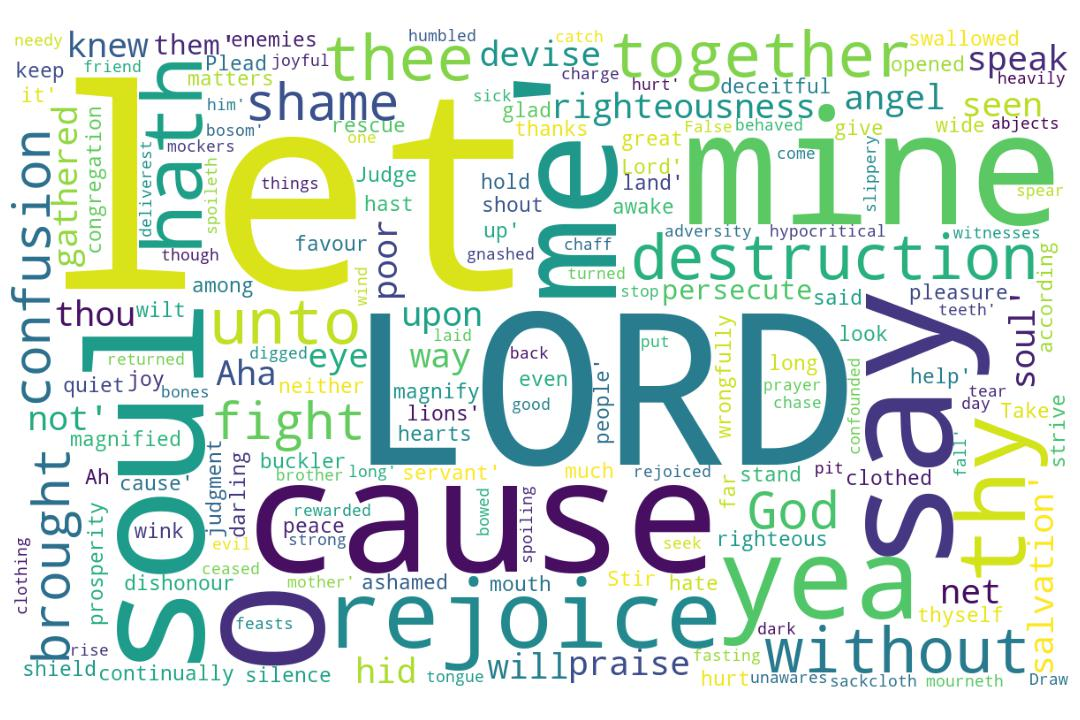
\includegraphics[width=\linewidth]{19OT-Psalms/Psalm35-WordCloud.jpg}
  \caption{Psalm 35 Word Cloud}
  \label{fig:Psalm 35 word Cloud}
\end{figure}

\marginpar{\scriptsize \centering \fcolorbox{bone}{lime}{\textbf{A HEARTFELT CRY}}\\ (Psalm 35:1--28) 
\begin{compactenum}[I.][8]
    \item A \textbf{Distinct  Petition} \index[scripture]{Psalms!Psa 035:24} (Psa 35:24)  (for enemies $\hdots$)
    \begin{compactenum}[A.][7]
		\item To be Confounded \index[scripture]{Psalms!Psa 035:04} (Psa 35:4)
		\item To be Confused \index[scripture]{Psalms!Psa 035:04}\index[scripture]{Psalms!Psa 035:26} (Psa 35:4, 26)
		\item To Become Chaff \index[scripture]{Psalms!Psa 035:05} (Psa 35:5)
		\item To be Chased \index[scripture]{Psalms!Psa 035:05} (Psa 35:5)
		\item To be Consumed \index[scripture]{Psalms!Psa 035:08} (Psa 35:8)
		\item To be Clothed in Shame \index[scripture]{Psalms!Psa 035:25} (Psa 35:25)
		\item To be Conquered \index[scripture]{Psalms!Psa 035:28} (Psa 35:28)
    \end{compactenum}
    \item A \textbf{Dangerous Prayer} \index[scripture]{Psalms!Psa 035:24} (Psa 35:24)
    \item A \textbf{Definite Promise} \index[scripture]{Psalms!Psa 035:28} (Psa 35:28)
\end{compactenum} }

\marginpar{\scriptsize \centering \fcolorbox{bone}{yellow}{\textbf{HELP, PLEASE!}}\\ (Psalm 35:1--28) 
\begin{compactenum}[I.][8]

    \item  The \textbf{Asking} \index[scripture]{Psalms!Psa 035:01} (Psa 35:1)  
    \item  \textbf{Admiration} \index[scripture]{Psalms!Psa 035:10} (Psa 35:10)  
    \item  \textbf{Adversity} \index[scripture]{Psalms!Psa 035:15} (Psa 35:15)  
    \item  \textbf{Abjects} \index[scripture]{Psalms!Psa 035:15} (Psa 35:15)  
    \item  \textbf{Adversaries} \index[scripture]{Psalms!Psa 035:15} (Psa 35:15)  
    \item  \textbf{Assembly} \index[scripture]{Psalms!Psa 035:18} (Psa 35:18)  
    \item  \textbf{Activation} \index[scripture]{Psalms!Psa 035:23} (Psa 35:23)  
    \item  \textbf{Acknowledgment} \index[scripture]{Psalms!Psa 035:27} (Psa 35:27)  
\end{compactenum} }

%%%%%%%%%%%%%%%%%%%%%%%%%%%%%%%%%%%%%%%%%%%%%%
%%%%%%%%%%%%%%%%%%%%%%%%%%%%%%%%%%%%%%%%%%%%%%
\footnote{\textcolor[cmyk]{0.99998,1,0,0}{\hyperlink{TOC}{Return to end of Table of Contents.}}}\footnote{\href{https://audiobible.com/bible}{\textcolor[cmyk]{0.99998,1,0,0}{Psalms Audio}}}\textcolor[cmyk]{0.99998,1,0,0}{Plead \emph{my} \emph{cause}, O LORD, with them that strive with me: fight against them that fight against me.}\marginpar{\scriptsize \textcolor[rgb]{0.00,0.545,0.269}{$\rightarrow$(1) Strife [1], (2) Shield [2], (3) Spear [3], (4) Salvation [3], (5) Shame [4], (6) Slipping [6], (7) Spoiling [10].}}
[2] \textcolor[cmyk]{0.99998,1,0,0}{Take hold of shield and buckler, and stand up for mine help.}
[3] \textcolor[cmyk]{0.99998,1,0,0}{Draw out also the spear, and stop \emph{the} \emph{way} against them that persecute me: say unto my soul, I \emph{am} thy salvation.}
[4] \textcolor[cmyk]{0.99998,1,0,0}{Let them be \fcolorbox{bone}{lime}{confounded} and put to shame that seek after my soul: let them be turned back and brought to \fcolorbox{bone}{lime}{confusion} that devise my hurt.}
[5] \textcolor[cmyk]{0.99998,1,0,0}{Let them be as \fcolorbox{bone}{lime}{chaff} before the wind: and let the angel of the LORD \fcolorbox{bone}{lime}{chase} \emph{them}.}
[6] \textcolor[cmyk]{0.99998,1,0,0}{Let their way be dark and slippery: and let the angel of the LORD persecute them.}
[7] \textcolor[cmyk]{0.99998,1,0,0}{For without cause have they hid for me their net \emph{in} a pit, \emph{which} without cause they have digged for my soul.}
[8] \textcolor[cmyk]{0.99998,1,0,0}{Let \fcolorbox{bone}{lime}{destruction} come upon him at unawares; and let his net that he hath hid catch himself: into that very destruction let him fall.}
[9] \textcolor[cmyk]{0.99998,1,0,0}{And my soul shall be joyful in the LORD: it shall rejoice in his salvation.}
[10] \textcolor[cmyk]{0.99998,1,0,0}{All my bones shall say, LORD, who \emph{is} like unto thee, which deliverest the poor from him that is too strong for him, yea, the poor and the needy from him that spoileth him?}
[11] \textcolor[cmyk]{0.99998,1,0,0}{False witnesses did rise up; they laid to my charge \emph{things} that I knew not.}
[12] \textcolor[cmyk]{0.99998,1,0,0}{They rewarded me evil for good \emph{to} the spoiling of my soul.}
[13] \textcolor[cmyk]{0.99998,1,0,0}{But as for me, when they were sick, my clothing \emph{was} sackcloth: I humbled my soul with fasting; and my prayer returned into mine own bosom.}
[14] \textcolor[cmyk]{0.99998,1,0,0}{I behaved myself as though \emph{he} \emph{had} \emph{been} my friend \emph{or} brother: I bowed down heavily, as one that mourneth \emph{for} \emph{his} mother.}
[15] \textcolor[cmyk]{0.99998,1,0,0}{But in mine adversity they rejoiced, and gathered themselves together: \emph{yea}, the abjects gathered themselves together against me, and I knew \emph{it} not; they did tear \emph{me}, and ceased not:}
[16] \textcolor[cmyk]{0.99998,1,0,0}{With hypocritical mockers in feasts, they gnashed upon me with their teeth.}
[17] \textcolor[cmyk]{0.99998,1,0,0}{Lord, how long wilt thou look on? rescue my soul from their destructions, my darling from the lions.}
[18] \textcolor[cmyk]{0.99998,1,0,0}{I will give thee thanks in the great congregation: I will praise thee among much people.}
[19] \textcolor[cmyk]{0.99998,1,0,0}{Let not them that are mine enemies wrongfully rejoice over me: \emph{neither} let them wink with the eye that hate me without a cause.}
[20] \textcolor[cmyk]{0.99998,1,0,0}{For they speak not peace: but they devise deceitful matters against \emph{them} \emph{that} \emph{are} quiet in the land.}
[21] \textcolor[cmyk]{0.99998,1,0,0}{Yea, they opened their mouth wide against me, \emph{and} said, Aha, aha, our eye hath seen \emph{it}.}
[22] \textcolor[cmyk]{0.99998,1,0,0}{\emph{This} thou hast seen, O LORD: keep not silence: O Lord, be not far from me.}
[23] \textcolor[cmyk]{0.99998,1,0,0}{Stir up thyself, and awake to my judgment, \emph{even} unto my cause, my God and my Lord.}
[24] \textcolor[cmyk]{0.99998,1,0,0}{\fcolorbox{bone}{lime}{Judge me}, O LORD my God, according to thy righteousness; and let them not rejoice over me.}
[25] \textcolor[cmyk]{0.99998,1,0,0}{Let them not say in their hearts, Ah, so would we have it: let them not say, We have swallowed him up.}
[26] \textcolor[cmyk]{0.99998,1,0,0}{Let them be ashamed and brought to confusion together that rejoice at mine hurt: let them be clothed with shame and dishonour that magnify \emph{themselves} against me.}
[27] \textcolor[cmyk]{0.99998,1,0,0}{Let them shout for joy, and be glad, that favour my righteous cause: yea, let them say continually, Let the LORD be magnified, which hath pleasure in the prosperity of his servant.}
[28] \textcolor[cmyk]{0.99998,1,0,0}{And my tongue \fcolorbox{bone}{lime}{shall speak} of thy righteousness \emph{and} of thy praise all the day long.}



\section{Psalm 35 Comments}

\subsection{Numeric Nuggets}
\textbf{13: } Verse 9, 18, and 23 have 13 unique words.
%\index[NWIV]{18!Psalms!Psa 35:1}\index[AWIP]{Plead!Psalms!Psa 35:1}\index[AWIP]{\emph{my}!Psalms!Psa 35:1}\index[AWIP]{\emph{cause}!Psalms!Psa 35:1}\index[AWIP]{O!Psalms!Psa 35:1}\index[AWIP]{LORD!Psalms!Psa 35:1}\index[AWIP]{with!Psalms!Psa 35:1}\index[AWIP]{with!Psalms!Psa 35:1 (2)}\index[AWIP]{them!Psalms!Psa 35:1}\index[AWIP]{them!Psalms!Psa 35:1 (2)}\index[AWIP]{that!Psalms!Psa 35:1}\index[AWIP]{that!Psalms!Psa 35:1 (2)}\index[AWIP]{strive!Psalms!Psa 35:1}\index[AWIP]{me!Psalms!Psa 35:1}\index[AWIP]{me!Psalms!Psa 35:1 (2)}\index[AWIP]{fight!Psalms!Psa 35:1}\index[AWIP]{fight!Psalms!Psa 35:1 (2)}\index[AWIP]{against!Psalms!Psa 35:1}\index[AWIP]{against!Psalms!Psa 35:1 (2)}\index[AWIP]{\emph{my}!Psalms!Psa 35:1}\index[AWIP]{\emph{cause}!Psalms!Psa 35:1}

\index[NWIV]{12!Psalms!Psa 35:2}\index[AWIP]{Take!Psalms!Psa 35:2}\index[AWIP]{hold!Psalms!Psa 35:2}\index[AWIP]{of!Psalms!Psa 35:2}\index[AWIP]{shield!Psalms!Psa 35:2}\index[AWIP]{and!Psalms!Psa 35:2}\index[AWIP]{and!Psalms!Psa 35:2 (2)}\index[AWIP]{buckler!Psalms!Psa 35:2}\index[AWIP]{stand!Psalms!Psa 35:2}\index[AWIP]{up!Psalms!Psa 35:2}\index[AWIP]{for!Psalms!Psa 35:2}\index[AWIP]{mine!Psalms!Psa 35:2}\index[AWIP]{help!Psalms!Psa 35:2}

\index[NWIV]{22!Psalms!Psa 35:3}\index[AWIP]{Draw!Psalms!Psa 35:3}\index[AWIP]{out!Psalms!Psa 35:3}\index[AWIP]{also!Psalms!Psa 35:3}\index[AWIP]{the!Psalms!Psa 35:3}\index[AWIP]{spear!Psalms!Psa 35:3}\index[AWIP]{and!Psalms!Psa 35:3}\index[AWIP]{stop!Psalms!Psa 35:3}\index[AWIP]{\emph{the}!Psalms!Psa 35:3}\index[AWIP]{\emph{way}!Psalms!Psa 35:3}\index[AWIP]{against!Psalms!Psa 35:3}\index[AWIP]{them!Psalms!Psa 35:3}\index[AWIP]{that!Psalms!Psa 35:3}\index[AWIP]{persecute!Psalms!Psa 35:3}\index[AWIP]{me!Psalms!Psa 35:3}\index[AWIP]{say!Psalms!Psa 35:3}\index[AWIP]{unto!Psalms!Psa 35:3}\index[AWIP]{my!Psalms!Psa 35:3}\index[AWIP]{soul!Psalms!Psa 35:3}\index[AWIP]{I!Psalms!Psa 35:3}\index[AWIP]{\emph{am}!Psalms!Psa 35:3}\index[AWIP]{thy!Psalms!Psa 35:3}\index[AWIP]{salvation!Psalms!Psa 35:3}\index[AWIP]{\emph{the}!Psalms!Psa 35:3}\index[AWIP]{\emph{way}!Psalms!Psa 35:3}\index[AWIP]{\emph{am}!Psalms!Psa 35:3}

\index[NWIV]{26!Psalms!Psa 35:4}\index[AWIP]{Let!Psalms!Psa 35:4}\index[AWIP]{them!Psalms!Psa 35:4}\index[AWIP]{them!Psalms!Psa 35:4 (2)}\index[AWIP]{be!Psalms!Psa 35:4}\index[AWIP]{be!Psalms!Psa 35:4 (2)}\index[AWIP]{confounded!Psalms!Psa 35:4}\index[AWIP]{and!Psalms!Psa 35:4}\index[AWIP]{and!Psalms!Psa 35:4 (2)}\index[AWIP]{put!Psalms!Psa 35:4}\index[AWIP]{to!Psalms!Psa 35:4}\index[AWIP]{to!Psalms!Psa 35:4 (2)}\index[AWIP]{shame!Psalms!Psa 35:4}\index[AWIP]{that!Psalms!Psa 35:4}\index[AWIP]{that!Psalms!Psa 35:4 (2)}\index[AWIP]{seek!Psalms!Psa 35:4}\index[AWIP]{after!Psalms!Psa 35:4}\index[AWIP]{my!Psalms!Psa 35:4}\index[AWIP]{my!Psalms!Psa 35:4 (2)}\index[AWIP]{soul!Psalms!Psa 35:4}\index[AWIP]{let!Psalms!Psa 35:4}\index[AWIP]{turned!Psalms!Psa 35:4}\index[AWIP]{back!Psalms!Psa 35:4}\index[AWIP]{brought!Psalms!Psa 35:4}\index[AWIP]{confusion!Psalms!Psa 35:4}\index[AWIP]{devise!Psalms!Psa 35:4}\index[AWIP]{hurt!Psalms!Psa 35:4}

\index[NWIV]{17!Psalms!Psa 35:5}\index[AWIP]{Let!Psalms!Psa 35:5}\index[AWIP]{them!Psalms!Psa 35:5}\index[AWIP]{be!Psalms!Psa 35:5}\index[AWIP]{as!Psalms!Psa 35:5}\index[AWIP]{chaff!Psalms!Psa 35:5}\index[AWIP]{before!Psalms!Psa 35:5}\index[AWIP]{the!Psalms!Psa 35:5}\index[AWIP]{the!Psalms!Psa 35:5 (2)}\index[AWIP]{the!Psalms!Psa 35:5 (3)}\index[AWIP]{wind!Psalms!Psa 35:5}\index[AWIP]{and!Psalms!Psa 35:5}\index[AWIP]{let!Psalms!Psa 35:5}\index[AWIP]{angel!Psalms!Psa 35:5}\index[AWIP]{of!Psalms!Psa 35:5}\index[AWIP]{LORD!Psalms!Psa 35:5}\index[AWIP]{chase!Psalms!Psa 35:5}\index[AWIP]{\emph{them}!Psalms!Psa 35:5}\index[AWIP]{\emph{them}!Psalms!Psa 35:5}

\index[NWIV]{16!Psalms!Psa 35:6}\index[AWIP]{Let!Psalms!Psa 35:6}\index[AWIP]{their!Psalms!Psa 35:6}\index[AWIP]{way!Psalms!Psa 35:6}\index[AWIP]{be!Psalms!Psa 35:6}\index[AWIP]{dark!Psalms!Psa 35:6}\index[AWIP]{and!Psalms!Psa 35:6}\index[AWIP]{and!Psalms!Psa 35:6 (2)}\index[AWIP]{slippery!Psalms!Psa 35:6}\index[AWIP]{let!Psalms!Psa 35:6}\index[AWIP]{the!Psalms!Psa 35:6}\index[AWIP]{the!Psalms!Psa 35:6 (2)}\index[AWIP]{angel!Psalms!Psa 35:6}\index[AWIP]{of!Psalms!Psa 35:6}\index[AWIP]{LORD!Psalms!Psa 35:6}\index[AWIP]{persecute!Psalms!Psa 35:6}\index[AWIP]{them!Psalms!Psa 35:6}

\index[NWIV]{22!Psalms!Psa 35:7}\index[AWIP]{For!Psalms!Psa 35:7}\index[AWIP]{without!Psalms!Psa 35:7}\index[AWIP]{without!Psalms!Psa 35:7 (2)}\index[AWIP]{cause!Psalms!Psa 35:7}\index[AWIP]{cause!Psalms!Psa 35:7 (2)}\index[AWIP]{have!Psalms!Psa 35:7}\index[AWIP]{have!Psalms!Psa 35:7 (2)}\index[AWIP]{they!Psalms!Psa 35:7}\index[AWIP]{they!Psalms!Psa 35:7 (2)}\index[AWIP]{hid!Psalms!Psa 35:7}\index[AWIP]{for!Psalms!Psa 35:7}\index[AWIP]{for!Psalms!Psa 35:7 (2)}\index[AWIP]{me!Psalms!Psa 35:7}\index[AWIP]{their!Psalms!Psa 35:7}\index[AWIP]{net!Psalms!Psa 35:7}\index[AWIP]{\emph{in}!Psalms!Psa 35:7}\index[AWIP]{a!Psalms!Psa 35:7}\index[AWIP]{pit!Psalms!Psa 35:7}\index[AWIP]{\emph{which}!Psalms!Psa 35:7}\index[AWIP]{digged!Psalms!Psa 35:7}\index[AWIP]{my!Psalms!Psa 35:7}\index[AWIP]{soul!Psalms!Psa 35:7}\index[AWIP]{\emph{in}!Psalms!Psa 35:7}\index[AWIP]{\emph{which}!Psalms!Psa 35:7}

\index[NWIV]{24!Psalms!Psa 35:8}\index[AWIP]{Let!Psalms!Psa 35:8}\index[AWIP]{destruction!Psalms!Psa 35:8}\index[AWIP]{destruction!Psalms!Psa 35:8 (2)}\index[AWIP]{come!Psalms!Psa 35:8}\index[AWIP]{upon!Psalms!Psa 35:8}\index[AWIP]{him!Psalms!Psa 35:8}\index[AWIP]{him!Psalms!Psa 35:8 (2)}\index[AWIP]{at!Psalms!Psa 35:8}\index[AWIP]{unawares!Psalms!Psa 35:8}\index[AWIP]{and!Psalms!Psa 35:8}\index[AWIP]{let!Psalms!Psa 35:8}\index[AWIP]{let!Psalms!Psa 35:8 (2)}\index[AWIP]{his!Psalms!Psa 35:8}\index[AWIP]{net!Psalms!Psa 35:8}\index[AWIP]{that!Psalms!Psa 35:8}\index[AWIP]{that!Psalms!Psa 35:8 (2)}\index[AWIP]{he!Psalms!Psa 35:8}\index[AWIP]{hath!Psalms!Psa 35:8}\index[AWIP]{hid!Psalms!Psa 35:8}\index[AWIP]{catch!Psalms!Psa 35:8}\index[AWIP]{himself!Psalms!Psa 35:8}\index[AWIP]{into!Psalms!Psa 35:8}\index[AWIP]{very!Psalms!Psa 35:8}\index[AWIP]{fall!Psalms!Psa 35:8}

\index[NWIV]{15!Psalms!Psa 35:9}\index[AWIP]{And!Psalms!Psa 35:9}\index[AWIP]{my!Psalms!Psa 35:9}\index[AWIP]{soul!Psalms!Psa 35:9}\index[AWIP]{shall!Psalms!Psa 35:9}\index[AWIP]{shall!Psalms!Psa 35:9 (2)}\index[AWIP]{be!Psalms!Psa 35:9}\index[AWIP]{joyful!Psalms!Psa 35:9}\index[AWIP]{in!Psalms!Psa 35:9}\index[AWIP]{in!Psalms!Psa 35:9 (2)}\index[AWIP]{the!Psalms!Psa 35:9}\index[AWIP]{LORD!Psalms!Psa 35:9}\index[AWIP]{it!Psalms!Psa 35:9}\index[AWIP]{rejoice!Psalms!Psa 35:9}\index[AWIP]{his!Psalms!Psa 35:9}\index[AWIP]{salvation!Psalms!Psa 35:9}

\index[NWIV]{34!Psalms!Psa 35:10}\index[AWIP]{All!Psalms!Psa 35:10}\index[AWIP]{my!Psalms!Psa 35:10}\index[AWIP]{bones!Psalms!Psa 35:10}\index[AWIP]{shall!Psalms!Psa 35:10}\index[AWIP]{say!Psalms!Psa 35:10}\index[AWIP]{LORD!Psalms!Psa 35:10}\index[AWIP]{who!Psalms!Psa 35:10}\index[AWIP]{\emph{is}!Psalms!Psa 35:10}\index[AWIP]{like!Psalms!Psa 35:10}\index[AWIP]{unto!Psalms!Psa 35:10}\index[AWIP]{thee!Psalms!Psa 35:10}\index[AWIP]{which!Psalms!Psa 35:10}\index[AWIP]{deliverest!Psalms!Psa 35:10}\index[AWIP]{the!Psalms!Psa 35:10}\index[AWIP]{the!Psalms!Psa 35:10 (2)}\index[AWIP]{the!Psalms!Psa 35:10 (3)}\index[AWIP]{poor!Psalms!Psa 35:10}\index[AWIP]{poor!Psalms!Psa 35:10 (2)}\index[AWIP]{from!Psalms!Psa 35:10}\index[AWIP]{from!Psalms!Psa 35:10 (2)}\index[AWIP]{him!Psalms!Psa 35:10}\index[AWIP]{him!Psalms!Psa 35:10 (2)}\index[AWIP]{him!Psalms!Psa 35:10 (3)}\index[AWIP]{that!Psalms!Psa 35:10}\index[AWIP]{that!Psalms!Psa 35:10 (2)}\index[AWIP]{is!Psalms!Psa 35:10}\index[AWIP]{too!Psalms!Psa 35:10}\index[AWIP]{strong!Psalms!Psa 35:10}\index[AWIP]{for!Psalms!Psa 35:10}\index[AWIP]{yea!Psalms!Psa 35:10}\index[AWIP]{and!Psalms!Psa 35:10}\index[AWIP]{needy!Psalms!Psa 35:10}\index[AWIP]{spoileth!Psalms!Psa 35:10}\index[AWIP]{him?!Psalms!Psa 35:10}\index[AWIP]{\emph{is}!Psalms!Psa 35:10}

\index[NWIV]{15!Psalms!Psa 35:11}\index[AWIP]{False!Psalms!Psa 35:11}\index[AWIP]{witnesses!Psalms!Psa 35:11}\index[AWIP]{did!Psalms!Psa 35:11}\index[AWIP]{rise!Psalms!Psa 35:11}\index[AWIP]{up!Psalms!Psa 35:11}\index[AWIP]{they!Psalms!Psa 35:11}\index[AWIP]{laid!Psalms!Psa 35:11}\index[AWIP]{to!Psalms!Psa 35:11}\index[AWIP]{my!Psalms!Psa 35:11}\index[AWIP]{charge!Psalms!Psa 35:11}\index[AWIP]{\emph{things}!Psalms!Psa 35:11}\index[AWIP]{that!Psalms!Psa 35:11}\index[AWIP]{I!Psalms!Psa 35:11}\index[AWIP]{knew!Psalms!Psa 35:11}\index[AWIP]{not!Psalms!Psa 35:11}\index[AWIP]{\emph{things}!Psalms!Psa 35:11}

\index[NWIV]{12!Psalms!Psa 35:12}\index[AWIP]{They!Psalms!Psa 35:12}\index[AWIP]{rewarded!Psalms!Psa 35:12}\index[AWIP]{me!Psalms!Psa 35:12}\index[AWIP]{evil!Psalms!Psa 35:12}\index[AWIP]{for!Psalms!Psa 35:12}\index[AWIP]{good!Psalms!Psa 35:12}\index[AWIP]{\emph{to}!Psalms!Psa 35:12}\index[AWIP]{the!Psalms!Psa 35:12}\index[AWIP]{spoiling!Psalms!Psa 35:12}\index[AWIP]{of!Psalms!Psa 35:12}\index[AWIP]{my!Psalms!Psa 35:12}\index[AWIP]{soul!Psalms!Psa 35:12}\index[AWIP]{\emph{to}!Psalms!Psa 35:12}

\index[NWIV]{26!Psalms!Psa 35:13}\index[AWIP]{But!Psalms!Psa 35:13}\index[AWIP]{as!Psalms!Psa 35:13}\index[AWIP]{for!Psalms!Psa 35:13}\index[AWIP]{me!Psalms!Psa 35:13}\index[AWIP]{when!Psalms!Psa 35:13}\index[AWIP]{they!Psalms!Psa 35:13}\index[AWIP]{were!Psalms!Psa 35:13}\index[AWIP]{sick!Psalms!Psa 35:13}\index[AWIP]{my!Psalms!Psa 35:13}\index[AWIP]{my!Psalms!Psa 35:13 (2)}\index[AWIP]{my!Psalms!Psa 35:13 (3)}\index[AWIP]{clothing!Psalms!Psa 35:13}\index[AWIP]{\emph{was}!Psalms!Psa 35:13}\index[AWIP]{sackcloth!Psalms!Psa 35:13}\index[AWIP]{I!Psalms!Psa 35:13}\index[AWIP]{humbled!Psalms!Psa 35:13}\index[AWIP]{soul!Psalms!Psa 35:13}\index[AWIP]{with!Psalms!Psa 35:13}\index[AWIP]{fasting!Psalms!Psa 35:13}\index[AWIP]{and!Psalms!Psa 35:13}\index[AWIP]{prayer!Psalms!Psa 35:13}\index[AWIP]{returned!Psalms!Psa 35:13}\index[AWIP]{into!Psalms!Psa 35:13}\index[AWIP]{mine!Psalms!Psa 35:13}\index[AWIP]{own!Psalms!Psa 35:13}\index[AWIP]{bosom!Psalms!Psa 35:13}\index[AWIP]{\emph{was}!Psalms!Psa 35:13}

\index[NWIV]{23!Psalms!Psa 35:14}\index[AWIP]{I!Psalms!Psa 35:14}\index[AWIP]{I!Psalms!Psa 35:14 (2)}\index[AWIP]{behaved!Psalms!Psa 35:14}\index[AWIP]{myself!Psalms!Psa 35:14}\index[AWIP]{as!Psalms!Psa 35:14}\index[AWIP]{as!Psalms!Psa 35:14 (2)}\index[AWIP]{though!Psalms!Psa 35:14}\index[AWIP]{\emph{he}!Psalms!Psa 35:14}\index[AWIP]{\emph{had}!Psalms!Psa 35:14}\index[AWIP]{\emph{been}!Psalms!Psa 35:14}\index[AWIP]{my!Psalms!Psa 35:14}\index[AWIP]{friend!Psalms!Psa 35:14}\index[AWIP]{\emph{or}!Psalms!Psa 35:14}\index[AWIP]{brother!Psalms!Psa 35:14}\index[AWIP]{bowed!Psalms!Psa 35:14}\index[AWIP]{down!Psalms!Psa 35:14}\index[AWIP]{heavily!Psalms!Psa 35:14}\index[AWIP]{one!Psalms!Psa 35:14}\index[AWIP]{that!Psalms!Psa 35:14}\index[AWIP]{mourneth!Psalms!Psa 35:14}\index[AWIP]{\emph{for}!Psalms!Psa 35:14}\index[AWIP]{\emph{his}!Psalms!Psa 35:14}\index[AWIP]{mother!Psalms!Psa 35:14}\index[AWIP]{\emph{he}!Psalms!Psa 35:14}\index[AWIP]{\emph{had}!Psalms!Psa 35:14}\index[AWIP]{\emph{been}!Psalms!Psa 35:14}\index[AWIP]{\emph{or}!Psalms!Psa 35:14}\index[AWIP]{\emph{for}!Psalms!Psa 35:14}\index[AWIP]{\emph{his}!Psalms!Psa 35:14}

\index[NWIV]{30!Psalms!Psa 35:15}\index[AWIP]{But!Psalms!Psa 35:15}\index[AWIP]{in!Psalms!Psa 35:15}\index[AWIP]{mine!Psalms!Psa 35:15}\index[AWIP]{adversity!Psalms!Psa 35:15}\index[AWIP]{they!Psalms!Psa 35:15}\index[AWIP]{they!Psalms!Psa 35:15 (2)}\index[AWIP]{rejoiced!Psalms!Psa 35:15}\index[AWIP]{and!Psalms!Psa 35:15}\index[AWIP]{and!Psalms!Psa 35:15 (2)}\index[AWIP]{and!Psalms!Psa 35:15 (3)}\index[AWIP]{gathered!Psalms!Psa 35:15}\index[AWIP]{gathered!Psalms!Psa 35:15 (2)}\index[AWIP]{themselves!Psalms!Psa 35:15}\index[AWIP]{themselves!Psalms!Psa 35:15 (2)}\index[AWIP]{together!Psalms!Psa 35:15}\index[AWIP]{together!Psalms!Psa 35:15 (2)}\index[AWIP]{\emph{yea}!Psalms!Psa 35:15}\index[AWIP]{the!Psalms!Psa 35:15}\index[AWIP]{abjects!Psalms!Psa 35:15}\index[AWIP]{against!Psalms!Psa 35:15}\index[AWIP]{me!Psalms!Psa 35:15}\index[AWIP]{I!Psalms!Psa 35:15}\index[AWIP]{knew!Psalms!Psa 35:15}\index[AWIP]{\emph{it}!Psalms!Psa 35:15}\index[AWIP]{not!Psalms!Psa 35:15}\index[AWIP]{not!Psalms!Psa 35:15 (2)}\index[AWIP]{did!Psalms!Psa 35:15}\index[AWIP]{tear!Psalms!Psa 35:15}\index[AWIP]{\emph{me}!Psalms!Psa 35:15}\index[AWIP]{ceased!Psalms!Psa 35:15}\index[AWIP]{\emph{yea}!Psalms!Psa 35:15}\index[AWIP]{\emph{it}!Psalms!Psa 35:15}\index[AWIP]{\emph{me}!Psalms!Psa 35:15}

\index[NWIV]{12!Psalms!Psa 35:16}\index[AWIP]{With!Psalms!Psa 35:16}\index[AWIP]{hypocritical!Psalms!Psa 35:16}\index[AWIP]{mockers!Psalms!Psa 35:16}\index[AWIP]{in!Psalms!Psa 35:16}\index[AWIP]{feasts!Psalms!Psa 35:16}\index[AWIP]{they!Psalms!Psa 35:16}\index[AWIP]{gnashed!Psalms!Psa 35:16}\index[AWIP]{upon!Psalms!Psa 35:16}\index[AWIP]{me!Psalms!Psa 35:16}\index[AWIP]{with!Psalms!Psa 35:16}\index[AWIP]{their!Psalms!Psa 35:16}\index[AWIP]{teeth!Psalms!Psa 35:16}

\index[NWIV]{18!Psalms!Psa 35:17}\index[AWIP]{Lord!Psalms!Psa 35:17}\index[AWIP]{how!Psalms!Psa 35:17}\index[AWIP]{long!Psalms!Psa 35:17}\index[AWIP]{wilt!Psalms!Psa 35:17}\index[AWIP]{thou!Psalms!Psa 35:17}\index[AWIP]{look!Psalms!Psa 35:17}\index[AWIP]{on?!Psalms!Psa 35:17}\index[AWIP]{rescue!Psalms!Psa 35:17}\index[AWIP]{my!Psalms!Psa 35:17}\index[AWIP]{my!Psalms!Psa 35:17 (2)}\index[AWIP]{soul!Psalms!Psa 35:17}\index[AWIP]{from!Psalms!Psa 35:17}\index[AWIP]{from!Psalms!Psa 35:17 (2)}\index[AWIP]{their!Psalms!Psa 35:17}\index[AWIP]{destructions!Psalms!Psa 35:17}\index[AWIP]{darling!Psalms!Psa 35:17}\index[AWIP]{the!Psalms!Psa 35:17}\index[AWIP]{lions!Psalms!Psa 35:17}

\index[NWIV]{16!Psalms!Psa 35:18}\index[AWIP]{I!Psalms!Psa 35:18}\index[AWIP]{I!Psalms!Psa 35:18 (2)}\index[AWIP]{will!Psalms!Psa 35:18}\index[AWIP]{will!Psalms!Psa 35:18 (2)}\index[AWIP]{give!Psalms!Psa 35:18}\index[AWIP]{thee!Psalms!Psa 35:18}\index[AWIP]{thee!Psalms!Psa 35:18 (2)}\index[AWIP]{thanks!Psalms!Psa 35:18}\index[AWIP]{in!Psalms!Psa 35:18}\index[AWIP]{the!Psalms!Psa 35:18}\index[AWIP]{great!Psalms!Psa 35:18}\index[AWIP]{congregation!Psalms!Psa 35:18}\index[AWIP]{praise!Psalms!Psa 35:18}\index[AWIP]{among!Psalms!Psa 35:18}\index[AWIP]{much!Psalms!Psa 35:18}\index[AWIP]{people!Psalms!Psa 35:18}

\index[NWIV]{24!Psalms!Psa 35:19}\index[AWIP]{Let!Psalms!Psa 35:19}\index[AWIP]{not!Psalms!Psa 35:19}\index[AWIP]{them!Psalms!Psa 35:19}\index[AWIP]{them!Psalms!Psa 35:19 (2)}\index[AWIP]{that!Psalms!Psa 35:19}\index[AWIP]{that!Psalms!Psa 35:19 (2)}\index[AWIP]{are!Psalms!Psa 35:19}\index[AWIP]{mine!Psalms!Psa 35:19}\index[AWIP]{enemies!Psalms!Psa 35:19}\index[AWIP]{wrongfully!Psalms!Psa 35:19}\index[AWIP]{rejoice!Psalms!Psa 35:19}\index[AWIP]{over!Psalms!Psa 35:19}\index[AWIP]{me!Psalms!Psa 35:19}\index[AWIP]{me!Psalms!Psa 35:19 (2)}\index[AWIP]{\emph{neither}!Psalms!Psa 35:19}\index[AWIP]{let!Psalms!Psa 35:19}\index[AWIP]{wink!Psalms!Psa 35:19}\index[AWIP]{with!Psalms!Psa 35:19}\index[AWIP]{the!Psalms!Psa 35:19}\index[AWIP]{eye!Psalms!Psa 35:19}\index[AWIP]{hate!Psalms!Psa 35:19}\index[AWIP]{without!Psalms!Psa 35:19}\index[AWIP]{a!Psalms!Psa 35:19}\index[AWIP]{cause!Psalms!Psa 35:19}\index[AWIP]{\emph{neither}!Psalms!Psa 35:19}

\index[NWIV]{18!Psalms!Psa 35:20}\index[AWIP]{For!Psalms!Psa 35:20}\index[AWIP]{they!Psalms!Psa 35:20}\index[AWIP]{they!Psalms!Psa 35:20 (2)}\index[AWIP]{speak!Psalms!Psa 35:20}\index[AWIP]{not!Psalms!Psa 35:20}\index[AWIP]{peace!Psalms!Psa 35:20}\index[AWIP]{but!Psalms!Psa 35:20}\index[AWIP]{devise!Psalms!Psa 35:20}\index[AWIP]{deceitful!Psalms!Psa 35:20}\index[AWIP]{matters!Psalms!Psa 35:20}\index[AWIP]{against!Psalms!Psa 35:20}\index[AWIP]{\emph{them}!Psalms!Psa 35:20}\index[AWIP]{\emph{that}!Psalms!Psa 35:20}\index[AWIP]{\emph{are}!Psalms!Psa 35:20}\index[AWIP]{quiet!Psalms!Psa 35:20}\index[AWIP]{in!Psalms!Psa 35:20}\index[AWIP]{the!Psalms!Psa 35:20}\index[AWIP]{land!Psalms!Psa 35:20}\index[AWIP]{\emph{them}!Psalms!Psa 35:20}\index[AWIP]{\emph{that}!Psalms!Psa 35:20}\index[AWIP]{\emph{are}!Psalms!Psa 35:20}

\index[NWIV]{17!Psalms!Psa 35:21}\index[AWIP]{Yea!Psalms!Psa 35:21}\index[AWIP]{they!Psalms!Psa 35:21}\index[AWIP]{opened!Psalms!Psa 35:21}\index[AWIP]{their!Psalms!Psa 35:21}\index[AWIP]{mouth!Psalms!Psa 35:21}\index[AWIP]{wide!Psalms!Psa 35:21}\index[AWIP]{against!Psalms!Psa 35:21}\index[AWIP]{me!Psalms!Psa 35:21}\index[AWIP]{\emph{and}!Psalms!Psa 35:21}\index[AWIP]{said!Psalms!Psa 35:21}\index[AWIP]{Aha!Psalms!Psa 35:21}\index[AWIP]{aha!Psalms!Psa 35:21}\index[AWIP]{our!Psalms!Psa 35:21}\index[AWIP]{eye!Psalms!Psa 35:21}\index[AWIP]{hath!Psalms!Psa 35:21}\index[AWIP]{seen!Psalms!Psa 35:21}\index[AWIP]{\emph{it}!Psalms!Psa 35:21}\index[AWIP]{\emph{and}!Psalms!Psa 35:21}\index[AWIP]{\emph{it}!Psalms!Psa 35:21}

\index[NWIV]{16!Psalms!Psa 35:22}\index[AWIP]{\emph{This}!Psalms!Psa 35:22}\index[AWIP]{thou!Psalms!Psa 35:22}\index[AWIP]{hast!Psalms!Psa 35:22}\index[AWIP]{seen!Psalms!Psa 35:22}\index[AWIP]{O!Psalms!Psa 35:22}\index[AWIP]{O!Psalms!Psa 35:22 (2)}\index[AWIP]{LORD!Psalms!Psa 35:22}\index[AWIP]{keep!Psalms!Psa 35:22}\index[AWIP]{not!Psalms!Psa 35:22}\index[AWIP]{not!Psalms!Psa 35:22 (2)}\index[AWIP]{silence!Psalms!Psa 35:22}\index[AWIP]{Lord!Psalms!Psa 35:22}\index[AWIP]{be!Psalms!Psa 35:22}\index[AWIP]{far!Psalms!Psa 35:22}\index[AWIP]{from!Psalms!Psa 35:22}\index[AWIP]{me!Psalms!Psa 35:22}\index[AWIP]{\emph{This}!Psalms!Psa 35:22}

\index[NWIV]{17!Psalms!Psa 35:23}\index[AWIP]{Stir!Psalms!Psa 35:23}\index[AWIP]{up!Psalms!Psa 35:23}\index[AWIP]{thyself!Psalms!Psa 35:23}\index[AWIP]{and!Psalms!Psa 35:23}\index[AWIP]{and!Psalms!Psa 35:23 (2)}\index[AWIP]{awake!Psalms!Psa 35:23}\index[AWIP]{to!Psalms!Psa 35:23}\index[AWIP]{my!Psalms!Psa 35:23}\index[AWIP]{my!Psalms!Psa 35:23 (2)}\index[AWIP]{my!Psalms!Psa 35:23 (3)}\index[AWIP]{my!Psalms!Psa 35:23 (4)}\index[AWIP]{judgment!Psalms!Psa 35:23}\index[AWIP]{\emph{even}!Psalms!Psa 35:23}\index[AWIP]{unto!Psalms!Psa 35:23}\index[AWIP]{cause!Psalms!Psa 35:23}\index[AWIP]{God!Psalms!Psa 35:23}\index[AWIP]{Lord!Psalms!Psa 35:23}\index[AWIP]{\emph{even}!Psalms!Psa 35:23}

\index[NWIV]{17!Psalms!Psa 35:24}\index[AWIP]{Judge!Psalms!Psa 35:24}\index[AWIP]{me!Psalms!Psa 35:24}\index[AWIP]{me!Psalms!Psa 35:24 (2)}\index[AWIP]{O!Psalms!Psa 35:24}\index[AWIP]{LORD!Psalms!Psa 35:24}\index[AWIP]{my!Psalms!Psa 35:24}\index[AWIP]{God!Psalms!Psa 35:24}\index[AWIP]{according!Psalms!Psa 35:24}\index[AWIP]{to!Psalms!Psa 35:24}\index[AWIP]{thy!Psalms!Psa 35:24}\index[AWIP]{righteousness!Psalms!Psa 35:24}\index[AWIP]{and!Psalms!Psa 35:24}\index[AWIP]{let!Psalms!Psa 35:24}\index[AWIP]{them!Psalms!Psa 35:24}\index[AWIP]{not!Psalms!Psa 35:24}\index[AWIP]{rejoice!Psalms!Psa 35:24}\index[AWIP]{over!Psalms!Psa 35:24}

\index[NWIV]{22!Psalms!Psa 35:25}\index[AWIP]{Let!Psalms!Psa 35:25}\index[AWIP]{them!Psalms!Psa 35:25}\index[AWIP]{them!Psalms!Psa 35:25 (2)}\index[AWIP]{not!Psalms!Psa 35:25}\index[AWIP]{not!Psalms!Psa 35:25 (2)}\index[AWIP]{say!Psalms!Psa 35:25}\index[AWIP]{say!Psalms!Psa 35:25 (2)}\index[AWIP]{in!Psalms!Psa 35:25}\index[AWIP]{their!Psalms!Psa 35:25}\index[AWIP]{hearts!Psalms!Psa 35:25}\index[AWIP]{Ah!Psalms!Psa 35:25}\index[AWIP]{so!Psalms!Psa 35:25}\index[AWIP]{would!Psalms!Psa 35:25}\index[AWIP]{we!Psalms!Psa 35:25}\index[AWIP]{have!Psalms!Psa 35:25}\index[AWIP]{have!Psalms!Psa 35:25 (2)}\index[AWIP]{it!Psalms!Psa 35:25}\index[AWIP]{let!Psalms!Psa 35:25}\index[AWIP]{We!Psalms!Psa 35:25}\index[AWIP]{swallowed!Psalms!Psa 35:25}\index[AWIP]{him!Psalms!Psa 35:25}\index[AWIP]{up!Psalms!Psa 35:25}

\index[NWIV]{27!Psalms!Psa 35:26}\index[AWIP]{Let!Psalms!Psa 35:26}\index[AWIP]{them!Psalms!Psa 35:26}\index[AWIP]{them!Psalms!Psa 35:26 (2)}\index[AWIP]{be!Psalms!Psa 35:26}\index[AWIP]{be!Psalms!Psa 35:26 (2)}\index[AWIP]{ashamed!Psalms!Psa 35:26}\index[AWIP]{and!Psalms!Psa 35:26}\index[AWIP]{and!Psalms!Psa 35:26 (2)}\index[AWIP]{brought!Psalms!Psa 35:26}\index[AWIP]{to!Psalms!Psa 35:26}\index[AWIP]{confusion!Psalms!Psa 35:26}\index[AWIP]{together!Psalms!Psa 35:26}\index[AWIP]{that!Psalms!Psa 35:26}\index[AWIP]{that!Psalms!Psa 35:26 (2)}\index[AWIP]{rejoice!Psalms!Psa 35:26}\index[AWIP]{at!Psalms!Psa 35:26}\index[AWIP]{mine!Psalms!Psa 35:26}\index[AWIP]{hurt!Psalms!Psa 35:26}\index[AWIP]{let!Psalms!Psa 35:26}\index[AWIP]{clothed!Psalms!Psa 35:26}\index[AWIP]{with!Psalms!Psa 35:26}\index[AWIP]{shame!Psalms!Psa 35:26}\index[AWIP]{dishonour!Psalms!Psa 35:26}\index[AWIP]{magnify!Psalms!Psa 35:26}\index[AWIP]{\emph{themselves}!Psalms!Psa 35:26}\index[AWIP]{against!Psalms!Psa 35:26}\index[AWIP]{me!Psalms!Psa 35:26}\index[AWIP]{\emph{themselves}!Psalms!Psa 35:26}

\index[NWIV]{32!Psalms!Psa 35:27}\index[AWIP]{Let!Psalms!Psa 35:27}\index[AWIP]{Let!Psalms!Psa 35:27 (2)}\index[AWIP]{them!Psalms!Psa 35:27}\index[AWIP]{them!Psalms!Psa 35:27 (2)}\index[AWIP]{shout!Psalms!Psa 35:27}\index[AWIP]{for!Psalms!Psa 35:27}\index[AWIP]{joy!Psalms!Psa 35:27}\index[AWIP]{and!Psalms!Psa 35:27}\index[AWIP]{be!Psalms!Psa 35:27}\index[AWIP]{be!Psalms!Psa 35:27 (2)}\index[AWIP]{glad!Psalms!Psa 35:27}\index[AWIP]{that!Psalms!Psa 35:27}\index[AWIP]{favour!Psalms!Psa 35:27}\index[AWIP]{my!Psalms!Psa 35:27}\index[AWIP]{righteous!Psalms!Psa 35:27}\index[AWIP]{cause!Psalms!Psa 35:27}\index[AWIP]{yea!Psalms!Psa 35:27}\index[AWIP]{let!Psalms!Psa 35:27}\index[AWIP]{say!Psalms!Psa 35:27}\index[AWIP]{continually!Psalms!Psa 35:27}\index[AWIP]{the!Psalms!Psa 35:27}\index[AWIP]{the!Psalms!Psa 35:27 (2)}\index[AWIP]{LORD!Psalms!Psa 35:27}\index[AWIP]{magnified!Psalms!Psa 35:27}\index[AWIP]{which!Psalms!Psa 35:27}\index[AWIP]{hath!Psalms!Psa 35:27}\index[AWIP]{pleasure!Psalms!Psa 35:27}\index[AWIP]{in!Psalms!Psa 35:27}\index[AWIP]{prosperity!Psalms!Psa 35:27}\index[AWIP]{of!Psalms!Psa 35:27}\index[AWIP]{his!Psalms!Psa 35:27}\index[AWIP]{servant!Psalms!Psa 35:27}

\index[NWIV]{16!Psalms!Psa 35:28}\index[AWIP]{And!Psalms!Psa 35:28}\index[AWIP]{my!Psalms!Psa 35:28}\index[AWIP]{tongue!Psalms!Psa 35:28}\index[AWIP]{shall!Psalms!Psa 35:28}\index[AWIP]{speak!Psalms!Psa 35:28}\index[AWIP]{of!Psalms!Psa 35:28}\index[AWIP]{of!Psalms!Psa 35:28 (2)}\index[AWIP]{thy!Psalms!Psa 35:28}\index[AWIP]{thy!Psalms!Psa 35:28 (2)}\index[AWIP]{righteousness!Psalms!Psa 35:28}\index[AWIP]{\emph{and}!Psalms!Psa 35:28}\index[AWIP]{praise!Psalms!Psa 35:28}\index[AWIP]{all!Psalms!Psa 35:28}\index[AWIP]{the!Psalms!Psa 35:28}\index[AWIP]{day!Psalms!Psa 35:28}\index[AWIP]{long!Psalms!Psa 35:28}\index[AWIP]{\emph{and}!Psalms!Psa 35:28}

%%%%%%%%%%%%%%%%%%%%%%%%%%%%%
%%%%%%%%%%%%%%%%%%%%%%%%%%%%%

\index[DOCTRINES]{Practicology - Sleep!Psalms!Psa 35:16}
\index[DOCTRINES]{Practicology - Straight Path!Psalms!Psa 35:11}
\index[DOCTRINES]{Practicology - Straight Path!Psalms!Psa 35:12}
\index[DOCTRINES]{Practicology - Straight Path!Psalms!Psa 35:14}
\index[DOCTRINES]{Practicology - Straight Path!Psalms!Psa 35:18}
\index[DOCTRINES]{Practicology - Straight Path!Psalms!Psa 35:27}


\section{Psalm 35 Outlines}

\subsection{My Outlines}

\subsubsection{A Heartfelt Cry}
\index[speaker]{Keith Anthony!Psalm 035 (A Heartfelt Cry)}
\index[series]{Psalms (Keith Anthony)!Psalm 035 (A Heartfelt Cry)}
\index[date]{2017/02/04!Psalm 035 (A Heartfelt Cry) (Keith Anthony)}
%\textbf{Introduction: }He was
\begin{compactenum}[I.][7]
    \item A \textbf{Distinct  Petition} \index[scripture]{Psalms!Psa 035:24} (Psa 35:24)  (for enemies $\hdots$)
    \begin{compactenum}[A.][7]
		\item To be Confounded \index[scripture]{Psalms!Psa 035:04} (Psa 35:4)
		\item To be Confused \index[scripture]{Psalms!Psa 035:04}\index[scripture]{Psalms!Psa 035:26} (Psa 35:4, 26)
		\item To Become Chaff \index[scripture]{Psalms!Psa 035:05} (Psa 35:5)
		\item To be Chased \index[scripture]{Psalms!Psa 035:05} (Psa 35:5)
		\item To be Consumed \index[scripture]{Psalms!Psa 035:08} (Psa 35:8)
		\item To be Clothed in Shame \index[scripture]{Psalms!Psa 035:25} (Psa 35:25)
		\item To be Conquered \index[scripture]{Psalms!Psa 035:28} (Psa 35:28)
    \end{compactenum}
    \item A \textbf{Dangerous Prayer} \index[scripture]{Psalms!Psa 035:24} (Psa 35:24)
    \item A \textbf{Definite Promise} \index[scripture]{Psalms!Psa 035:28} (Psa 35:28)
\end{compactenum}

\subsubsection{Help, Please}
\index[speaker]{Keith Anthony!Psalm 035 (Help, Please)}
\index[series]{Psalms (Keith Anthony)!Psalm 035 (Help, Please)}
\index[date]{2017/07/11!Psalm 035 (Help, Please) (Keith Anthony)}
%\textbf{Introduction: }He was
\begin{compactenum}[I.][7]
    \item  The \textbf{Asking} \index[scripture]{Psalms!Psa 035:01} (Psa 35:1)  
    \item  \textbf{Admiration} \index[scripture]{Psalms!Psa 035:10} (Psa 35:10)  
    \item  \textbf{Adversity} \index[scripture]{Psalms!Psa 035:15} (Psa 35:15)  
    \item  \textbf{Abjects} \index[scripture]{Psalms!Psa 035:15} (Psa 35:15)  
    \item  \textbf{Adversaries} \index[scripture]{Psalms!Psa 035:15} (Psa 35:15)  
    \item  \textbf{Assembly} \index[scripture]{Psalms!Psa 035:18} (Psa 35:18)  
    \item  \textbf{Activation} \index[scripture]{Psalms!Psa 035:23} (Psa 35:23)  
    \item  \textbf{Acknowledgment} \index[scripture]{Psalms!Psa 035:27} (Psa 35:27)  
\end{compactenum}

\subsection{Outlines from Others}
%\section{Psalm 35 Statistics}

%%%%%%%%%%%%%%%%%%%%%%%%%%%
%%%%% Word Statistics
%%%%%%%%%%%%%%%%%%%%%%%%%%


\normalsize



\subsection{Chapter Word Statistics}


%%%%%%%%%%
%%%%%%%%%%
 
\begin{center}
\begin{longtable}{l|c|c|c|c}
\caption[Stats for Psalm 35]{Stats for Psalm 35} \label{table:Stats for Psalm 35} \\ 
\hline \multicolumn{1}{|c|}{\textbf{Verse(s)}} & \multicolumn{1}{|c|}{\textbf{Count}} & \multicolumn{1}{|c|}{\textbf{Unique}} & \multicolumn{1}{|c|}{\textbf{Italics}} & \multicolumn{1}{|c|}{\textbf{Uniq Italic}}  \\ \hline 
\endfirsthead
 
\multicolumn{5}{c}
{{\bfseries \tablename\ \thetable{} -- continued from previous page}} \\  
\hline \multicolumn{1}{|c|}{\textbf{Verse(s)}} & \multicolumn{1}{|c|}{\textbf{Count}} & \multicolumn{1}{|c|}{\textbf{Unique}} & \multicolumn{1}{|c|}{\textbf{Italics}} & \multicolumn{1}{|c|}{\textbf{Uniq Italic}}  \\ \hline 
\endhead
 
\hline \multicolumn{5}{|r|}{{Continued if needed}} \\ \hline
\endfoot 
1 & 18 & 12 & 2 & 2\\ \hline
2 & 12 & 11 & 0 & 0\\ \hline
3 & 22 & 22 & 3 & 3\\ \hline
4 & 26 & 20 & 0 & 0\\ \hline
5 & 17 & 15 & 1 & 1\\ \hline
6 & 16 & 14 & 0 & 0\\ \hline
7 & 22 & 17 & 2 & 2\\ \hline
8 & 24 & 20 & 0 & 0\\ \hline
9 & 15 & 13 & 0 & 0\\ \hline
10 & 34 & 26 & 1 & 1\\ \hline
11 & 15 & 15 & 1 & 1\\ \hline
12 & 12 & 12 & 1 & 1\\ \hline
13 & 26 & 24 & 1 & 1\\ \hline
14 & 23 & 21 & 6 & 6\\ \hline
15 & 30 & 23 & 3 & 3\\ \hline
16 & 12 & 12 & 0 & 0\\ \hline
17 & 18 & 16 & 0 & 0\\ \hline
18 & 16 & 13 & 0 & 0\\ \hline
19 & 24 & 21 & 1 & 1\\ \hline
20 & 18 & 17 & 3 & 3\\ \hline
21 & 17 & 17 & 2 & 2\\ \hline
22 & 16 & 14 & 1 & 1\\ \hline
23 & 17 & 13 & 1 & 1\\ \hline
24 & 17 & 16 & 0 & 0\\ \hline
25 & 22 & 18 & 0 & 0\\ \hline
26 & 27 & 23 & 1 & 1\\ \hline
27 & 32 & 28 & 0 & 0\\ \hline
28 & 16 & 14 & 1 & 1\\ \hline
\hline \hline
Total & 564 & 262 & 31 & 28



\end{longtable}
\end{center}

%%%%%%%%%%
%%%%%%%%%%
 
\subsection{Words by Frequency}

\begin{center}
\begin{longtable}{l|r}
\caption[Word Frequencies in Psalm 35]{Word Frequencies in Psalm 35} \label{table:WordsIn-Psalm-35} \\ 
\hline \multicolumn{1}{|c|}{\textbf{Word}} & \multicolumn{1}{c|}{\textbf{Frequency}} \\ \hline 
\endfirsthead
 
\multicolumn{2}{c}
{{\bfseries \tablename\ \thetable{} -- continued from previous page}} \\ 
\hline \multicolumn{1}{|c|}{\textbf{Word}} & \multicolumn{1}{c|}{\textbf{Frequency}} \\ \hline 
\endhead
 
\hline \multicolumn{2}{|r|}{{Continued if needed}} \\ \hline
\endfoot
 
\hline \hline
\endlastfoot
my & 21 \\ \hline
and & 20 \\ \hline
the & 19 \\ \hline
them & 16 \\ \hline
that & 16 \\ \hline
me & 15 \\ \hline
be & 10 \\ \hline
let & 10 \\ \hline
they & 10 \\ \hline
not & 10 \\ \hline
Let & 9 \\ \hline
LORD & 8 \\ \hline
I & 8 \\ \hline
in & 8 \\ \hline
against & 7 \\ \hline
of & 7 \\ \hline
for & 7 \\ \hline
soul & 7 \\ \hline
him & 7 \\ \hline
with & 6 \\ \hline
to & 6 \\ \hline
their & 6 \\ \hline
mine & 5 \\ \hline
say & 5 \\ \hline
cause & 5 \\ \hline
from & 5 \\ \hline
O & 4 \\ \hline
up & 4 \\ \hline
thy & 4 \\ \hline
as & 4 \\ \hline
have & 4 \\ \hline
shall & 4 \\ \hline
rejoice & 4 \\ \hline
unto & 3 \\ \hline
without & 3 \\ \hline
his & 3 \\ \hline
hath & 3 \\ \hline
thee & 3 \\ \hline
together & 3 \\ \hline
Lord & 3 \\ \hline
fight & 2 \\ \hline
persecute & 2 \\ \hline
salvation & 2 \\ \hline
shame & 2 \\ \hline
brought & 2 \\ \hline
confusion & 2 \\ \hline
devise & 2 \\ \hline
hurt & 2 \\ \hline
angel & 2 \\ \hline
\emph{them} & 2 \\ \hline
For & 2 \\ \hline
hid & 2 \\ \hline
net & 2 \\ \hline
a & 2 \\ \hline
destruction & 2 \\ \hline
upon & 2 \\ \hline
at & 2 \\ \hline
into & 2 \\ \hline
And & 2 \\ \hline
it & 2 \\ \hline
which & 2 \\ \hline
poor & 2 \\ \hline
yea & 2 \\ \hline
did & 2 \\ \hline
knew & 2 \\ \hline
But & 2 \\ \hline
gathered & 2 \\ \hline
themselves & 2 \\ \hline
\emph{it} & 2 \\ \hline
long & 2 \\ \hline
thou & 2 \\ \hline
will & 2 \\ \hline
praise & 2 \\ \hline
over & 2 \\ \hline
eye & 2 \\ \hline
speak & 2 \\ \hline
\emph{and} & 2 \\ \hline
seen & 2 \\ \hline
God & 2 \\ \hline
righteousness & 2 \\ \hline
Plead & 1 \\ \hline
\emph{my} & 1 \\ \hline
\emph{cause} & 1 \\ \hline
strive & 1 \\ \hline
Take & 1 \\ \hline
hold & 1 \\ \hline
shield & 1 \\ \hline
buckler & 1 \\ \hline
stand & 1 \\ \hline
help & 1 \\ \hline
Draw & 1 \\ \hline
out & 1 \\ \hline
also & 1 \\ \hline
spear & 1 \\ \hline
stop & 1 \\ \hline
\emph{the} & 1 \\ \hline
\emph{way} & 1 \\ \hline
\emph{am} & 1 \\ \hline
confounded & 1 \\ \hline
put & 1 \\ \hline
seek & 1 \\ \hline
after & 1 \\ \hline
turned & 1 \\ \hline
back & 1 \\ \hline
chaff & 1 \\ \hline
before & 1 \\ \hline
wind & 1 \\ \hline
chase & 1 \\ \hline
way & 1 \\ \hline
dark & 1 \\ \hline
slippery & 1 \\ \hline
\emph{in} & 1 \\ \hline
pit & 1 \\ \hline
\emph{which} & 1 \\ \hline
digged & 1 \\ \hline
come & 1 \\ \hline
unawares & 1 \\ \hline
he & 1 \\ \hline
catch & 1 \\ \hline
himself & 1 \\ \hline
very & 1 \\ \hline
fall & 1 \\ \hline
joyful & 1 \\ \hline
All & 1 \\ \hline
bones & 1 \\ \hline
who & 1 \\ \hline
\emph{is} & 1 \\ \hline
like & 1 \\ \hline
deliverest & 1 \\ \hline
is & 1 \\ \hline
too & 1 \\ \hline
strong & 1 \\ \hline
needy & 1 \\ \hline
spoileth & 1 \\ \hline
False & 1 \\ \hline
witnesses & 1 \\ \hline
rise & 1 \\ \hline
laid & 1 \\ \hline
charge & 1 \\ \hline
\emph{things} & 1 \\ \hline
They & 1 \\ \hline
rewarded & 1 \\ \hline
evil & 1 \\ \hline
good & 1 \\ \hline
\emph{to} & 1 \\ \hline
spoiling & 1 \\ \hline
when & 1 \\ \hline
were & 1 \\ \hline
sick & 1 \\ \hline
clothing & 1 \\ \hline
\emph{was} & 1 \\ \hline
sackcloth & 1 \\ \hline
humbled & 1 \\ \hline
fasting & 1 \\ \hline
prayer & 1 \\ \hline
returned & 1 \\ \hline
own & 1 \\ \hline
bosom & 1 \\ \hline
behaved & 1 \\ \hline
myself & 1 \\ \hline
though & 1 \\ \hline
\emph{he} & 1 \\ \hline
\emph{had} & 1 \\ \hline
\emph{been} & 1 \\ \hline
friend & 1 \\ \hline
\emph{or} & 1 \\ \hline
brother & 1 \\ \hline
bowed & 1 \\ \hline
down & 1 \\ \hline
heavily & 1 \\ \hline
one & 1 \\ \hline
mourneth & 1 \\ \hline
\emph{for} & 1 \\ \hline
\emph{his} & 1 \\ \hline
mother & 1 \\ \hline
adversity & 1 \\ \hline
rejoiced & 1 \\ \hline
\emph{yea} & 1 \\ \hline
abjects & 1 \\ \hline
tear & 1 \\ \hline
\emph{me} & 1 \\ \hline
ceased & 1 \\ \hline
With & 1 \\ \hline
hypocritical & 1 \\ \hline
mockers & 1 \\ \hline
feasts & 1 \\ \hline
gnashed & 1 \\ \hline
teeth & 1 \\ \hline
how & 1 \\ \hline
wilt & 1 \\ \hline
look & 1 \\ \hline
on & 1 \\ \hline
rescue & 1 \\ \hline
destructions & 1 \\ \hline
darling & 1 \\ \hline
lions & 1 \\ \hline
give & 1 \\ \hline
thanks & 1 \\ \hline
great & 1 \\ \hline
congregation & 1 \\ \hline
among & 1 \\ \hline
much & 1 \\ \hline
people & 1 \\ \hline
are & 1 \\ \hline
enemies & 1 \\ \hline
wrongfully & 1 \\ \hline
\emph{neither} & 1 \\ \hline
wink & 1 \\ \hline
hate & 1 \\ \hline
peace & 1 \\ \hline
but & 1 \\ \hline
deceitful & 1 \\ \hline
matters & 1 \\ \hline
\emph{that} & 1 \\ \hline
\emph{are} & 1 \\ \hline
quiet & 1 \\ \hline
land & 1 \\ \hline
Yea & 1 \\ \hline
opened & 1 \\ \hline
mouth & 1 \\ \hline
wide & 1 \\ \hline
said & 1 \\ \hline
Aha & 1 \\ \hline
aha & 1 \\ \hline
our & 1 \\ \hline
\emph{This} & 1 \\ \hline
hast & 1 \\ \hline
keep & 1 \\ \hline
silence & 1 \\ \hline
far & 1 \\ \hline
Stir & 1 \\ \hline
thyself & 1 \\ \hline
awake & 1 \\ \hline
judgment & 1 \\ \hline
\emph{even} & 1 \\ \hline
Judge & 1 \\ \hline
according & 1 \\ \hline
hearts & 1 \\ \hline
Ah & 1 \\ \hline
so & 1 \\ \hline
would & 1 \\ \hline
we & 1 \\ \hline
We & 1 \\ \hline
swallowed & 1 \\ \hline
ashamed & 1 \\ \hline
clothed & 1 \\ \hline
dishonour & 1 \\ \hline
magnify & 1 \\ \hline
\emph{themselves} & 1 \\ \hline
shout & 1 \\ \hline
joy & 1 \\ \hline
glad & 1 \\ \hline
favour & 1 \\ \hline
righteous & 1 \\ \hline
continually & 1 \\ \hline
magnified & 1 \\ \hline
pleasure & 1 \\ \hline
prosperity & 1 \\ \hline
servant & 1 \\ \hline
tongue & 1 \\ \hline
all & 1 \\ \hline
day & 1 \\ \hline
\end{longtable}
\end{center}



\normalsize



\subsection{Words Alphabetically}

\begin{center}
\begin{longtable}{l|r}
\caption[Word Alphabetically in Psalm 35]{Word Alphabetically in Psalm 35} \label{table:WordsIn-Psalm-35} \\ 
\hline \multicolumn{1}{|c|}{\textbf{Word}} & \multicolumn{1}{c|}{\textbf{Frequency}} \\ \hline 
\endfirsthead
 
\multicolumn{2}{c}
{{\bfseries \tablename\ \thetable{} -- continued from previous page}} \\ 
\hline \multicolumn{1}{|c|}{\textbf{Word}} & \multicolumn{1}{c|}{\textbf{Frequency}} \\ \hline 
\endhead
 
\hline \multicolumn{2}{|r|}{{Continued if needed}} \\ \hline
\endfoot
 
\hline \hline
\endlastfoot
Ah & 1 \\ \hline
Aha & 1 \\ \hline
All & 1 \\ \hline
And & 2 \\ \hline
But & 2 \\ \hline
Draw & 1 \\ \hline
False & 1 \\ \hline
For & 2 \\ \hline
God & 2 \\ \hline
I & 8 \\ \hline
Judge & 1 \\ \hline
LORD & 8 \\ \hline
Let & 9 \\ \hline
Lord & 3 \\ \hline
O & 4 \\ \hline
Plead & 1 \\ \hline
Stir & 1 \\ \hline
Take & 1 \\ \hline
They & 1 \\ \hline
We & 1 \\ \hline
With & 1 \\ \hline
Yea & 1 \\ \hline
\emph{This} & 1 \\ \hline
\emph{am} & 1 \\ \hline
\emph{and} & 2 \\ \hline
\emph{are} & 1 \\ \hline
\emph{been} & 1 \\ \hline
\emph{cause} & 1 \\ \hline
\emph{even} & 1 \\ \hline
\emph{for} & 1 \\ \hline
\emph{had} & 1 \\ \hline
\emph{he} & 1 \\ \hline
\emph{his} & 1 \\ \hline
\emph{in} & 1 \\ \hline
\emph{is} & 1 \\ \hline
\emph{it} & 2 \\ \hline
\emph{me} & 1 \\ \hline
\emph{my} & 1 \\ \hline
\emph{neither} & 1 \\ \hline
\emph{or} & 1 \\ \hline
\emph{that} & 1 \\ \hline
\emph{themselves} & 1 \\ \hline
\emph{them} & 2 \\ \hline
\emph{the} & 1 \\ \hline
\emph{things} & 1 \\ \hline
\emph{to} & 1 \\ \hline
\emph{was} & 1 \\ \hline
\emph{way} & 1 \\ \hline
\emph{which} & 1 \\ \hline
\emph{yea} & 1 \\ \hline
a & 2 \\ \hline
abjects & 1 \\ \hline
according & 1 \\ \hline
adversity & 1 \\ \hline
after & 1 \\ \hline
against & 7 \\ \hline
aha & 1 \\ \hline
all & 1 \\ \hline
also & 1 \\ \hline
among & 1 \\ \hline
and & 20 \\ \hline
angel & 2 \\ \hline
are & 1 \\ \hline
as & 4 \\ \hline
ashamed & 1 \\ \hline
at & 2 \\ \hline
awake & 1 \\ \hline
back & 1 \\ \hline
be & 10 \\ \hline
before & 1 \\ \hline
behaved & 1 \\ \hline
bones & 1 \\ \hline
bosom & 1 \\ \hline
bowed & 1 \\ \hline
brother & 1 \\ \hline
brought & 2 \\ \hline
buckler & 1 \\ \hline
but & 1 \\ \hline
catch & 1 \\ \hline
cause & 5 \\ \hline
ceased & 1 \\ \hline
chaff & 1 \\ \hline
charge & 1 \\ \hline
chase & 1 \\ \hline
clothed & 1 \\ \hline
clothing & 1 \\ \hline
come & 1 \\ \hline
confounded & 1 \\ \hline
confusion & 2 \\ \hline
congregation & 1 \\ \hline
continually & 1 \\ \hline
dark & 1 \\ \hline
darling & 1 \\ \hline
day & 1 \\ \hline
deceitful & 1 \\ \hline
deliverest & 1 \\ \hline
destruction & 2 \\ \hline
destructions & 1 \\ \hline
devise & 2 \\ \hline
did & 2 \\ \hline
digged & 1 \\ \hline
dishonour & 1 \\ \hline
down & 1 \\ \hline
enemies & 1 \\ \hline
evil & 1 \\ \hline
eye & 2 \\ \hline
fall & 1 \\ \hline
far & 1 \\ \hline
fasting & 1 \\ \hline
favour & 1 \\ \hline
feasts & 1 \\ \hline
fight & 2 \\ \hline
for & 7 \\ \hline
friend & 1 \\ \hline
from & 5 \\ \hline
gathered & 2 \\ \hline
give & 1 \\ \hline
glad & 1 \\ \hline
gnashed & 1 \\ \hline
good & 1 \\ \hline
great & 1 \\ \hline
hast & 1 \\ \hline
hate & 1 \\ \hline
hath & 3 \\ \hline
have & 4 \\ \hline
he & 1 \\ \hline
hearts & 1 \\ \hline
heavily & 1 \\ \hline
help & 1 \\ \hline
hid & 2 \\ \hline
him & 7 \\ \hline
himself & 1 \\ \hline
his & 3 \\ \hline
hold & 1 \\ \hline
how & 1 \\ \hline
humbled & 1 \\ \hline
hurt & 2 \\ \hline
hypocritical & 1 \\ \hline
in & 8 \\ \hline
into & 2 \\ \hline
is & 1 \\ \hline
it & 2 \\ \hline
joy & 1 \\ \hline
joyful & 1 \\ \hline
judgment & 1 \\ \hline
keep & 1 \\ \hline
knew & 2 \\ \hline
laid & 1 \\ \hline
land & 1 \\ \hline
let & 10 \\ \hline
like & 1 \\ \hline
lions & 1 \\ \hline
long & 2 \\ \hline
look & 1 \\ \hline
magnified & 1 \\ \hline
magnify & 1 \\ \hline
matters & 1 \\ \hline
me & 15 \\ \hline
mine & 5 \\ \hline
mockers & 1 \\ \hline
mother & 1 \\ \hline
mourneth & 1 \\ \hline
mouth & 1 \\ \hline
much & 1 \\ \hline
my & 21 \\ \hline
myself & 1 \\ \hline
needy & 1 \\ \hline
net & 2 \\ \hline
not & 10 \\ \hline
of & 7 \\ \hline
on & 1 \\ \hline
one & 1 \\ \hline
opened & 1 \\ \hline
our & 1 \\ \hline
out & 1 \\ \hline
over & 2 \\ \hline
own & 1 \\ \hline
peace & 1 \\ \hline
people & 1 \\ \hline
persecute & 2 \\ \hline
pit & 1 \\ \hline
pleasure & 1 \\ \hline
poor & 2 \\ \hline
praise & 2 \\ \hline
prayer & 1 \\ \hline
prosperity & 1 \\ \hline
put & 1 \\ \hline
quiet & 1 \\ \hline
rejoice & 4 \\ \hline
rejoiced & 1 \\ \hline
rescue & 1 \\ \hline
returned & 1 \\ \hline
rewarded & 1 \\ \hline
righteous & 1 \\ \hline
righteousness & 2 \\ \hline
rise & 1 \\ \hline
sackcloth & 1 \\ \hline
said & 1 \\ \hline
salvation & 2 \\ \hline
say & 5 \\ \hline
seek & 1 \\ \hline
seen & 2 \\ \hline
servant & 1 \\ \hline
shall & 4 \\ \hline
shame & 2 \\ \hline
shield & 1 \\ \hline
shout & 1 \\ \hline
sick & 1 \\ \hline
silence & 1 \\ \hline
slippery & 1 \\ \hline
so & 1 \\ \hline
soul & 7 \\ \hline
speak & 2 \\ \hline
spear & 1 \\ \hline
spoileth & 1 \\ \hline
spoiling & 1 \\ \hline
stand & 1 \\ \hline
stop & 1 \\ \hline
strive & 1 \\ \hline
strong & 1 \\ \hline
swallowed & 1 \\ \hline
tear & 1 \\ \hline
teeth & 1 \\ \hline
thanks & 1 \\ \hline
that & 16 \\ \hline
the & 19 \\ \hline
thee & 3 \\ \hline
their & 6 \\ \hline
them & 16 \\ \hline
themselves & 2 \\ \hline
they & 10 \\ \hline
thou & 2 \\ \hline
though & 1 \\ \hline
thy & 4 \\ \hline
thyself & 1 \\ \hline
to & 6 \\ \hline
together & 3 \\ \hline
tongue & 1 \\ \hline
too & 1 \\ \hline
turned & 1 \\ \hline
unawares & 1 \\ \hline
unto & 3 \\ \hline
up & 4 \\ \hline
upon & 2 \\ \hline
very & 1 \\ \hline
way & 1 \\ \hline
we & 1 \\ \hline
were & 1 \\ \hline
when & 1 \\ \hline
which & 2 \\ \hline
who & 1 \\ \hline
wide & 1 \\ \hline
will & 2 \\ \hline
wilt & 1 \\ \hline
wind & 1 \\ \hline
wink & 1 \\ \hline
with & 6 \\ \hline
without & 3 \\ \hline
witnesses & 1 \\ \hline
would & 1 \\ \hline
wrongfully & 1 \\ \hline
yea & 2 \\ \hline
\end{longtable}
\end{center}



\normalsize



\subsection{Word Lengths in Chapter}
\normalsize
\begin{longtable}{l|p{3.75in}}
\caption[Words by Length in Psalm 35]{Words by Length in Psalm 35} \label{table:WordsIn-Psalm-35} \\ 
\hline \multicolumn{1}{|c|}{\textbf{Length}} & \multicolumn{1}{c|}{\textbf{Words}} \\ \hline 
\endfirsthead
 
\multicolumn{2}{c}
{{\bfseries \tablename\ \thetable{} -- continued from previous page}} \\ 
\hline \multicolumn{1}{|c|}{\textbf{Length}} & \multicolumn{1}{c|}{\textbf{Words}} \\ \hline 
\endhead
 
\hline \multicolumn{2}{|r|}{{Continued if needed}} \\ \hline
\endfoot
 
\hline \hline
\endlastfoot
1 & O, I, a \\ \hline
2 & \emph{my}, me, of, up, my, \emph{am}, be, to, as, \emph{in}, at, he, in, it, \emph{is}, is, \emph{to}, \emph{he}, \emph{or}, \emph{it}, \emph{me}, on, Ah, so, we, We \\ \hline
3 & and, for, out, the, \emph{the}, \emph{way}, say, thy, Let, put, let, way, For, hid, net, pit, him, his, And, All, who, too, yea, did, not, But, \emph{was}, own, \emph{had}, one, \emph{for}, \emph{his}, \emph{yea}, how, are, eye, but, \emph{are}, Yea, \emph{and}, Aha, aha, our, far, God, joy, all, day \\ \hline
4 & LORD, with, them, that, Take, hold, mine, help, Draw, also, stop, unto, soul, seek, back, hurt, wind, \emph{them}, dark, have, they, come, upon, hath, into, very, fall, like, thee, poor, from, rise, laid, knew, They, evil, good, when, were, sick, \emph{been}, down, tear, With, Lord, long, wilt, thou, look, will, give, much, over, wink, hate, \emph{that}, land, wide, said, seen, \emph{This}, hast, keep, Stir, \emph{even}, glad \\ \hline
5 & Plead, \emph{cause}, fight, stand, spear, shame, after, chaff, angel, chase, their, cause, \emph{which}, catch, shall, bones, which, needy, False, bosom, bowed, teeth, lions, great, among, speak, peace, quiet, mouth, awake, Judge, would, shout \\ \hline
6 & strive, shield, turned, devise, before, digged, joyful, strong, charge, \emph{things}, prayer, myself, though, friend, mother, ceased, feasts, rescue, thanks, praise, people, opened, hearts, favour, tongue \\ \hline
7 & against, buckler, brought, without, himself, rejoice, humbled, fasting, behaved, brother, heavily, abjects, mockers, gnashed, darling, enemies, \emph{neither}, matters, silence, thyself, ashamed, clothed, magnify, servant \\ \hline
8 & slippery, unawares, spoileth, rewarded, spoiling, clothing, returned, mourneth, rejoiced, gathered, together, judgment, pleasure \\ \hline
9 & persecute, salvation, confusion, witnesses, sackcloth, adversity, deceitful, according, swallowed, dishonour, righteous, magnified \\ \hline
10 & confounded, deliverest, themselves, wrongfully, \emph{themselves}, prosperity \\ \hline
11 & destruction, continually \\ \hline
12 & hypocritical, destructions, congregation \\ \hline
13 & righteousness \\ \hline
\end{longtable}






%%%%%%%%%%
%%%%%%%%%%
 



%%%%%%%%%%
%%%%%%%%%%
\subsection{Verses with 18 Words in Chapter}
\normalsize
\begin{longtable}{l|p{3.75in}}
\caption[Verses with 18 Words  in Psalm 35]{Verses with 18 Words  in Psalm 35} \label{table:Verses with 18 Words in-Psalm-35} \\ 
\hline \multicolumn{1}{|c|}{\textbf{Reference}} & \multicolumn{1}{c|}{\textbf{Verse}} \\ \hline 
\endfirsthead
 
\multicolumn{2}{c}
{{\bfseries \tablename\ \thetable{} -- continued from previous page}} \\ 
\hline \multicolumn{1}{|c|}{\textbf{Reference}} & \multicolumn{1}{c|}{\textbf{Verse}} \\ \hline 
\endhead
 
\hline \multicolumn{2}{|r|}{{Continued if needed}} \\ \hline
\endfoot
 
\hline \hline
\endlastfoot
Psalms 035:1 & Plead \emph{my} \emph{cause}, O LORD, with them that strive with me: fight against them that fight against me. \\ \hline
Psalms 035:17 & Lord, how long wilt thou look on? rescue my soul from their destructions, my darling from the lions. \\ \hline
Psalms 035:20 & For they speak not peace: but they devise deceitful matters against \emph{them} \emph{that} \emph{are} quiet in the land. \\ \hline
\end{longtable}






%%%%%%%%%%
%%%%%%%%%%
\subsection{Psalm 35 Repeated Phrases}


%%%%%%%%%%
%%%%%%%%%%
\normalsize
 
\begin{center}
\begin{longtable}{|p{3.0in}|p{0.5in}|}
\caption[Psalm 35 Repeated Phrases]{Psalm 35 Repeated Phrases}\label{table:Repeated Phrases Psalm 35} \\
\hline \multicolumn{1}{|c|}{\textbf{Phrase}} & \multicolumn{1}{c|}{\textbf{Frequency}} \\ \hline 
\endfirsthead
 
\multicolumn{2}{c}
{{\bfseries \tablename\ \thetable{} -- continued from previous page}} \\  
\hline \multicolumn{1}{|c|}{\textbf{Phrase}} & \multicolumn{1}{c|}{\textbf{Frequency}} \\ \hline 
\endhead
 
\hline \multicolumn{2}{c}{{ }} \\ \hline
\endfoot 
my soul & 7\\ \hline 
let them & 6\\ \hline 
Let them & 5\\ \hline 
them be & 5\\ \hline 
them that & 4\\ \hline 
against me & 4\\ \hline 
and let & 4\\ \hline 
the LORD & 4\\ \hline 
in the & 4\\ \hline 
O LORD & 3\\ \hline 
Let them be & 3\\ \hline 
them not & 3\\ \hline 
\end{longtable}
\end{center}



%%%%%%%%%%
%%%%%%%%%%




\chapter{Psalm 36}

\begin{figure}
  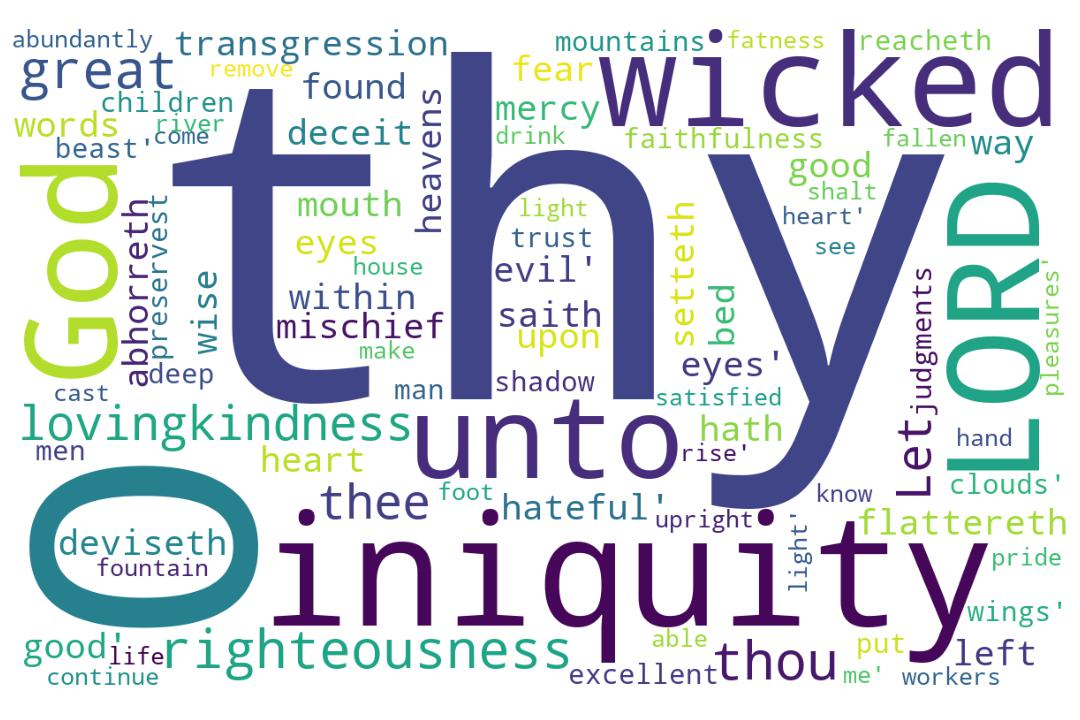
\includegraphics[width=\linewidth]{19OT-Psalms/Psalm36-WordCloud.jpg}
  \caption{Psalm 36 Word Cloud}
  \label{fig:Psalm 36 word Cloud}
\end{figure}
%%%%%%%%%%%%%%%%%%%%%%%%%%%%%%%%%%%%%%%%%
%%%%%%%%%%%%%%%%%%%%%%%%%%%%%%%%%%%%%%%%%

\marginpar{\scriptsize \centering \fcolorbox{bone}{lime}{\textbf{THE WICKED \& THE FAITHFUL}}\\ (Psalm 36:1-12) 
\begin{compactenum}[I.][8]
    \item The Wicked Have No \textbf{No Fear of God} \index[scripture]{Psalms!Psa 036:01} ( Psa 36:01)
    \item The Wicked Practice \textbf{Self Flattery} \index[scripture]{Psalms!Psa 036:02} (Psa 36:2)
    \item The Wicked Miss the \textbf{Faithfulness of God} \index[scripture]{Psalms!Psa 036:05} (Psa 36:05)
    \item The Faithful Partake of the \textbf{Fatness of God's House} \index[scripture]{Psalms!Psa 036:08} (Psa 36:08)
    \item The Faithful Partake of the \textbf{Fountain of Life} \index[scripture]{Psalms!Psa 036:09} (Psa 36:09)
    \item The Faithful are Delivered from the \textbf{Foot of Pride} and the Hand of the Wicked \index[scripture]{Psalms!Psa 036:11} (Psa 36:11)
    \item The Wicked will \textbf{Fall and Not Rise} \index[scripture]{Psalms!Psa 036:12} (Psa 36:12)
\end{compactenum} }

\marginpar{\scriptsize \centering \fcolorbox{bone}{yellow}{\textbf{THE WICKED \& THE RIGHTEOUS}}\\ (Psalm 36:1-12) 
\begin{compactenum}[I.][8]
    \item \textbf{Direction} of the Wicked \index[scripture]{Psalms!Psa 036:02} (Psa 36:2)
    \item \textbf{Deceit} of the Wicked \index[scripture]{Psalms!Psa 036:03} (Psa 36:3)
    \item \textbf{Devices} of the Wicked \index[scripture]{Psalms!Psa 036:04} (Psa 36:4)
    \item \textbf{Distinction} of the Righteous \index[scripture]{Psalms!Psa 036:05}\index[scripture]{Psalms!Psa 036:06} (Psa 36:5, 6)
    \item \textbf{Decision} of the Righteous \index[scripture]{Psalms!Psa 036:07}\index[scripture]{Psalms!Psa 036:08}\index[scripture]{Psalms!Psa 036:09} (Psa 36:7, 8, 9)
    \item \textbf{Deliverance} of the Righteous \index[scripture]{Psalms!Psa 036:10} (Psa 36:10)
    \item \textbf{Deeds} of the Wicked \index[scripture]{Psalms!Psa 036:12} (Psa 36:12)
    \item \textbf{Destination} of the Wicked \index[scripture]{Psalms!Psa 036:12} (Psa 36:12)
\end{compactenum} }

\marginpar{\scriptsize \centering \fcolorbox{bone}{black}{\textcolor{white}{\textbf{7 SINS OF THE WICKED}}}\\ (Psalm 36:1-12) 
\begin{compactenum}[I.][8]
    \item Has no \textbf{Fear of God} \index[scripture]{Psalms!Psa 036:01} (Psa 36:1)
    \item Exercises \textbf{Self-flattery} \index[scripture]{Psalms!Psa 036:02} (Psa 36:2)
    \item Chooses \textbf{Iniquity}  \index[scripture]{Psalms!Psa 036:02} \index[scripture]{Psalms!Psa 036:03} (Psa 36:2, 3)
    \item Practice \textbf{Deceit} \index[scripture]{Psalms!Psa 036:03} (Psa 36:3)
    \item Rejects \textbf{Wisdom} \index[scripture]{Psalms!Psa 036:03} (Psa 36:3)
    \item Pursues \textbf{Mischief} \index[scripture]{Psalms!Psa 036:04} (Psa 36:4)
    \item Does not \textbf{Abhor Evil} \index[scripture]{Psalms!Psa 036:05} (Psa 36:5)
\end{compactenum} }

\footnote{\textcolor[cmyk]{0.99998,1,0,0}{\hyperlink{TOC}{Return to end of Table of Contents.}}}\footnote{\href{https://audiobible.com/bible}{\textcolor[cmyk]{0.99998,1,0,0}{Psalms Audio}}}\textcolor[cmyk]{0.99998,1,0,0}{To the chief Musician, \emph{A Psalm} of David the servant of the LORD.}\\
\\
\textcolor[cmyk]{0.99998,1,0,0}{The \fcolorbox{bone}{MYGOLD}{transgression} of the wicked saith within my heart, \emph{that} \emph{there} \emph{is} \fcolorbox{bone}{lime}{no fear} of God before his eyes.}
[2] \textcolor[cmyk]{0.99998,1,0,0}{For he \fcolorbox{bone}{lime}{flattereth} himself in his own eyes, until his iniquity be found to be hateful.}
[3] \textcolor[cmyk]{0.99998,1,0,0}{The words of his mouth \emph{are} iniquity and deceit: he hath left off to be wise, \emph{and} to do good.}
[4] \textcolor[cmyk]{0.99998,1,0,0}{He deviseth mischief upon his bed; he setteth himself in a way \emph{that} \emph{is} not good; he abhorreth not evil.}
[5] \textcolor[cmyk]{0.99998,1,0,0}{Thy mercy, O LORD, \emph{is} in the heavens; \emph{and} thy \fcolorbox{bone}{lime}{faithfulness} \emph{reacheth} unto the clouds.}
[6] \textcolor[cmyk]{0.99998,1,0,0}{Thy \fcolorbox{bone}{MYGOLD}{righteousness} \emph{is} like the great mountains; thy judgments \emph{are} a great deep: O LORD, thou preservest man and beast.}
[7] \textcolor[cmyk]{0.99998,1,0,0}{How excellent \emph{is} thy lovingkindness, O God! therefore the children of men put their trust under the shadow of thy wings.}
[8] \textcolor[cmyk]{0.99998,1,0,0}{They shall be abundantly satisfied with the \fcolorbox{bone}{lime}{fatness} of thy house; and thou shalt make them drink of the river of thy pleasures.}
[9] \textcolor[cmyk]{0.99998,1,0,0}{For with thee \emph{is} the \fcolorbox{bone}{lime}{fountain} of life: in thy light shall we see light.}\footnote{\textbf{Proverb 13:14} - The law of the wise is a fountain of life, to depart from the snares of death.}\footnote{\textbf{Proverb 14:27} - The fear of the LORD is a fountain of life, to depart from the snares of death.}
[10] \textcolor[cmyk]{0.99998,1,0,0}{O continue thy lovingkindness unto them that know thee; and thy \fcolorbox{bone}{MYGOLD}{righteousness} to the upright in heart.}
[11] \textcolor[cmyk]{0.99998,1,0,0}{Let not the \fcolorbox{bone}{lime}{foot} of pride come against me, and let not the hand of the wicked remove me.}
[12] \textcolor[cmyk]{0.99998,1,0,0}{There are the workers of iniquity \fcolorbox{bone}{lime}{fallen}: they are cast down, and shall not be able to rise.}




\section{Psalm 36 Comments}

\subsection{Numeric Nuggets}
\textbf{13: } There are two 13-letter words in Psalm 36: ``transgression'' and ``righteousness.''
%\input{19OT-Psalms/Psalm36-WordIndex}
\section{Psalm 36 Outlines}

\subsection{My Outlines}

\subsubsection{The Wicked and the Faithful}
\index[speaker]{Keith Anthony!Psalm 036 (The Wicked and the Faithful)}
\index[series]{Psalms (Keith Anthony)!Psalm 036 (The Wicked and the Faithful)}
\index[date]{2016/12/14!Psalm 036 (The Wicked and the Faithful) (Keith Anthony)}
David describes the backdrop of evil and evil men, but contrasts it with the deliverance of God and his attributes working on behalf of the faithful:
\begin{compactenum}[I.]
    \item The Wicked Have No \textbf{No Fear of God} (\index[scripture]{Psalms!Psa 036:01}Psalm 36:01)
    \item The Wicked Practice \textbf{Self Flattery} (\index[scripture]{Psalms!Psa 036:02}Psalm 36:2)
    \item The Wicked Miss the \textbf{Faithfulness of God} \index[scripture]{Psalms!Psa 036:05} (Psalm 36:05)
    \item The Faithful Partake of the \textbf{Fatness of God's House} \index[scripture]{Psalms!Psa 036:08} (Psalm 36:08)
    \item The Faithful Partake of the \textbf{Fountain of Life} \index[scripture]{Psalms!Psa 036:09} (Psalm 36:09)
    \item The Faithful are Delivered from the \textbf{Foot of Pride} and the Hand of the Wicked \index[scripture]{Psalms!Psa 036:11} (Psalm 36:11)
    \item The Wicked will \textbf{Fall and Not Rise} \index[scripture]{Psalms!Psa 036:12} (Psalm 36:12)\end{compactenum}


\subsubsection{The Wicked \& the Righteous}
\index[speaker]{Keith Anthony!Psalm 036 (The Wicked \& the Righteous)}
\index[series]{Psalms (Keith Anthony)!Psalm 036 (The Wicked \& the Righteous)}
\index[date]{2017/07/12!Psalm 036 (The Wicked \& the Righteous (Keith Anthony)}

\begin{compactenum}[I.]
    \item \textbf{Direction} of the Wicked \index[scripture]{Psalms!Psa 036:02} (Psa 36:2)
    \item \textbf{Deceit} of the Wicked \index[scripture]{Psalms!Psa 036:03} (Psa 36:3)
    \item \textbf{Devices} of the Wicked \index[scripture]{Psalms!Psa 036:04} (Psa 36:4)
    \item \textbf{Distinction} of the Righteous \index[scripture]{Psalms!Psa 036:05}\index[scripture]{Psalms!Psa 036:06} (Psa 36:5, 6)
    \item \textbf{Decision} of the Righteous \index[scripture]{Psalms!Psa 036:07}\index[scripture]{Psalms!Psa 036:08}\index[scripture]{Psalms!Psa 036:09} (Psa 36:7, 8, 9)
    \item \textbf{Deliverance} of the Righteous \index[scripture]{Psalms!Psa 036:10} (Psa 36:10)
    \item \textbf{Deeds} of the Wicked \index[scripture]{Psalms!Psa 036:12} (Psa 36:12)
    \item \textbf{Destination} of the Wicked \index[scripture]{Psalms!Psa 036:12} (Psa 36:12)
\end{compactenum}



\subsubsection{7 Sins of The Wicked}
\index[speaker]{Keith Anthony!Psalm 036 (7 Sins of The Wicked)}
\index[series]{Psalms (Keith Anthony)!Psalm 036 (7 Sins of The Wicked)}
\index[date]{2021/02/05!Psalm 036 (7 Sins of The Wicked) (Keith Anthony)}

\begin{compactenum}[I.][8]
    \item Has no \textbf{Fear of God} \index[scripture]{Psalms!Psa 036:01} (Psa 36:1)
    \item Exercises \textbf{Self-flattery} \index[scripture]{Psalms!Psa 036:02} (Psa 36:2)
    \item Chooses \textbf{Iniquity}  \index[scripture]{Psalms!Psa 036:02} \index[scripture]{Psalms!Psa 036:03} (Psa 36:2, 3)
    \item Practice \textbf{Deceit} \index[scripture]{Psalms!Psa 036:03} (Psa 36:3)
    \item Rejects \textbf{Wisdom} \index[scripture]{Psalms!Psa 036:03} (Psa 36:3)
    \item Pursues \textbf{Mischief} \index[scripture]{Psalms!Psa 036:04} (Psa 36:4)
    \item Does not \textbf{Abhor Evil} \index[scripture]{Psalms!Psa 036:05} (Psa 36:5)
\end{compactenum} 

\subsection{Outlines from Others}
%\section{Psalm 36 Statistics}

%%%%%%%%%%%%%%%%%%%%%%%%%%%
%%%%% Word Statistics
%%%%%%%%%%%%%%%%%%%%%%%%%%


\normalsize



\subsection{Chapter Word Statistics}


%%%%%%%%%%
%%%%%%%%%%
 
\begin{center}
\begin{longtable}{l|c|c|c|c}
\caption[Stats for Psalm 36]{Stats for Psalm 36} \label{table:Stats for Psalm 36} \\ 
\hline \multicolumn{1}{|c|}{\textbf{Verse(s)}} & \multicolumn{1}{|c|}{\textbf{Count}} & \multicolumn{1}{|c|}{\textbf{Unique}} & \multicolumn{1}{|c|}{\textbf{Italics}} & \multicolumn{1}{|c|}{\textbf{Uniq Italic}}  \\ \hline 
\endfirsthead
 
\multicolumn{5}{c}
{{\bfseries \tablename\ \thetable{} -- continued from previous page}} \\  
\hline \multicolumn{1}{|c|}{\textbf{Verse(s)}} & \multicolumn{1}{|c|}{\textbf{Count}} & \multicolumn{1}{|c|}{\textbf{Unique}} & \multicolumn{1}{|c|}{\textbf{Italics}} & \multicolumn{1}{|c|}{\textbf{Uniq Italic}}  \\ \hline 
\endhead
 
\hline \multicolumn{5}{|r|}{{Continued if needed}} \\ \hline
\endfoot 
1 & 19 & 18 & 3 & 3\\ \hline
2 & 16 & 14 & 0 & 0\\ \hline
3 & 20 & 19 & 2 & 2\\ \hline
4 & 20 & 18 & 2 & 2\\ \hline
5 & 15 & 14 & 3 & 3\\ \hline
6 & 20 & 19 & 2 & 2\\ \hline
7 & 21 & 18 & 1 & 1\\ \hline
8 & 23 & 19 & 0 & 0\\ \hline
9 & 15 & 14 & 1 & 1\\ \hline
10 & 17 & 16 & 0 & 0\\ \hline
11 & 19 & 14 & 0 & 0\\ \hline
12 & 18 & 17 & 0 & 0\\ \hline
\hline \hline
Total & 223 & 126 & 14 & 6



\end{longtable}
\end{center}

%%%%%%%%%%
%%%%%%%%%%
 
\subsection{Words by Frequency}

\begin{center}
\begin{longtable}{l|r}
\caption[Word Frequencies in Psalm 36]{Word Frequencies in Psalm 36} \label{table:WordsIn-Psalm-36} \\ 
\hline \multicolumn{1}{|c|}{\textbf{Word}} & \multicolumn{1}{c|}{\textbf{Frequency}} \\ \hline 
\endfirsthead
 
\multicolumn{2}{c}
{{\bfseries \tablename\ \thetable{} -- continued from previous page}} \\ 
\hline \multicolumn{1}{|c|}{\textbf{Word}} & \multicolumn{1}{c|}{\textbf{Frequency}} \\ \hline 
\endhead
 
\hline \multicolumn{2}{|r|}{{Continued if needed}} \\ \hline
\endfoot
 
\hline \hline
\endlastfoot
the & 14 \\ \hline
of & 12 \\ \hline
thy & 9 \\ \hline
\emph{is} & 6 \\ \hline
and & 6 \\ \hline
his & 5 \\ \hline
in & 5 \\ \hline
be & 5 \\ \hline
to & 5 \\ \hline
not & 5 \\ \hline
he & 4 \\ \hline
O & 4 \\ \hline
iniquity & 3 \\ \hline
shall & 3 \\ \hline
The & 2 \\ \hline
wicked & 2 \\ \hline
heart & 2 \\ \hline
\emph{that} & 2 \\ \hline
God & 2 \\ \hline
eyes & 2 \\ \hline
For & 2 \\ \hline
himself & 2 \\ \hline
\emph{are} & 2 \\ \hline
\emph{and} & 2 \\ \hline
good & 2 \\ \hline
a & 2 \\ \hline
Thy & 2 \\ \hline
LORD & 2 \\ \hline
unto & 2 \\ \hline
righteousness & 2 \\ \hline
great & 2 \\ \hline
thou & 2 \\ \hline
lovingkindness & 2 \\ \hline
with & 2 \\ \hline
them & 2 \\ \hline
thee & 2 \\ \hline
light & 2 \\ \hline
me & 2 \\ \hline
are & 2 \\ \hline
transgression & 1 \\ \hline
saith & 1 \\ \hline
within & 1 \\ \hline
my & 1 \\ \hline
\emph{there} & 1 \\ \hline
no & 1 \\ \hline
fear & 1 \\ \hline
before & 1 \\ \hline
flattereth & 1 \\ \hline
own & 1 \\ \hline
until & 1 \\ \hline
found & 1 \\ \hline
hateful & 1 \\ \hline
words & 1 \\ \hline
mouth & 1 \\ \hline
deceit & 1 \\ \hline
hath & 1 \\ \hline
left & 1 \\ \hline
off & 1 \\ \hline
wise & 1 \\ \hline
do & 1 \\ \hline
He & 1 \\ \hline
deviseth & 1 \\ \hline
mischief & 1 \\ \hline
upon & 1 \\ \hline
bed & 1 \\ \hline
setteth & 1 \\ \hline
way & 1 \\ \hline
abhorreth & 1 \\ \hline
evil & 1 \\ \hline
mercy & 1 \\ \hline
heavens & 1 \\ \hline
faithfulness & 1 \\ \hline
\emph{reacheth} & 1 \\ \hline
clouds & 1 \\ \hline
like & 1 \\ \hline
mountains & 1 \\ \hline
judgments & 1 \\ \hline
deep & 1 \\ \hline
preservest & 1 \\ \hline
man & 1 \\ \hline
beast & 1 \\ \hline
How & 1 \\ \hline
excellent & 1 \\ \hline
therefore & 1 \\ \hline
children & 1 \\ \hline
men & 1 \\ \hline
put & 1 \\ \hline
their & 1 \\ \hline
trust & 1 \\ \hline
under & 1 \\ \hline
shadow & 1 \\ \hline
wings & 1 \\ \hline
They & 1 \\ \hline
abundantly & 1 \\ \hline
satisfied & 1 \\ \hline
fatness & 1 \\ \hline
house & 1 \\ \hline
shalt & 1 \\ \hline
make & 1 \\ \hline
drink & 1 \\ \hline
river & 1 \\ \hline
pleasures & 1 \\ \hline
fountain & 1 \\ \hline
life & 1 \\ \hline
we & 1 \\ \hline
see & 1 \\ \hline
continue & 1 \\ \hline
that & 1 \\ \hline
know & 1 \\ \hline
upright & 1 \\ \hline
Let & 1 \\ \hline
foot & 1 \\ \hline
pride & 1 \\ \hline
come & 1 \\ \hline
against & 1 \\ \hline
let & 1 \\ \hline
hand & 1 \\ \hline
remove & 1 \\ \hline
There & 1 \\ \hline
workers & 1 \\ \hline
fallen & 1 \\ \hline
they & 1 \\ \hline
cast & 1 \\ \hline
down & 1 \\ \hline
able & 1 \\ \hline
rise & 1 \\ \hline
\end{longtable}
\end{center}



\normalsize



\subsection{Words Alphabetically}

\begin{center}
\begin{longtable}{l|r}
\caption[Word Alphabetically in Psalm 36]{Word Alphabetically in Psalm 36} \label{table:WordsIn-Psalm-36} \\ 
\hline \multicolumn{1}{|c|}{\textbf{Word}} & \multicolumn{1}{c|}{\textbf{Frequency}} \\ \hline 
\endfirsthead
 
\multicolumn{2}{c}
{{\bfseries \tablename\ \thetable{} -- continued from previous page}} \\ 
\hline \multicolumn{1}{|c|}{\textbf{Word}} & \multicolumn{1}{c|}{\textbf{Frequency}} \\ \hline 
\endhead
 
\hline \multicolumn{2}{|r|}{{Continued if needed}} \\ \hline
\endfoot
 
\hline \hline
\endlastfoot
For & 2 \\ \hline
God & 2 \\ \hline
He & 1 \\ \hline
How & 1 \\ \hline
LORD & 2 \\ \hline
Let & 1 \\ \hline
O & 4 \\ \hline
The & 2 \\ \hline
There & 1 \\ \hline
They & 1 \\ \hline
Thy & 2 \\ \hline
\emph{and} & 2 \\ \hline
\emph{are} & 2 \\ \hline
\emph{is} & 6 \\ \hline
\emph{reacheth} & 1 \\ \hline
\emph{that} & 2 \\ \hline
\emph{there} & 1 \\ \hline
a & 2 \\ \hline
abhorreth & 1 \\ \hline
able & 1 \\ \hline
abundantly & 1 \\ \hline
against & 1 \\ \hline
and & 6 \\ \hline
are & 2 \\ \hline
be & 5 \\ \hline
beast & 1 \\ \hline
bed & 1 \\ \hline
before & 1 \\ \hline
cast & 1 \\ \hline
children & 1 \\ \hline
clouds & 1 \\ \hline
come & 1 \\ \hline
continue & 1 \\ \hline
deceit & 1 \\ \hline
deep & 1 \\ \hline
deviseth & 1 \\ \hline
do & 1 \\ \hline
down & 1 \\ \hline
drink & 1 \\ \hline
evil & 1 \\ \hline
excellent & 1 \\ \hline
eyes & 2 \\ \hline
faithfulness & 1 \\ \hline
fallen & 1 \\ \hline
fatness & 1 \\ \hline
fear & 1 \\ \hline
flattereth & 1 \\ \hline
foot & 1 \\ \hline
found & 1 \\ \hline
fountain & 1 \\ \hline
good & 2 \\ \hline
great & 2 \\ \hline
hand & 1 \\ \hline
hateful & 1 \\ \hline
hath & 1 \\ \hline
he & 4 \\ \hline
heart & 2 \\ \hline
heavens & 1 \\ \hline
himself & 2 \\ \hline
his & 5 \\ \hline
house & 1 \\ \hline
in & 5 \\ \hline
iniquity & 3 \\ \hline
judgments & 1 \\ \hline
know & 1 \\ \hline
left & 1 \\ \hline
let & 1 \\ \hline
life & 1 \\ \hline
light & 2 \\ \hline
like & 1 \\ \hline
lovingkindness & 2 \\ \hline
make & 1 \\ \hline
man & 1 \\ \hline
me & 2 \\ \hline
men & 1 \\ \hline
mercy & 1 \\ \hline
mischief & 1 \\ \hline
mountains & 1 \\ \hline
mouth & 1 \\ \hline
my & 1 \\ \hline
no & 1 \\ \hline
not & 5 \\ \hline
of & 12 \\ \hline
off & 1 \\ \hline
own & 1 \\ \hline
pleasures & 1 \\ \hline
preservest & 1 \\ \hline
pride & 1 \\ \hline
put & 1 \\ \hline
remove & 1 \\ \hline
righteousness & 2 \\ \hline
rise & 1 \\ \hline
river & 1 \\ \hline
saith & 1 \\ \hline
satisfied & 1 \\ \hline
see & 1 \\ \hline
setteth & 1 \\ \hline
shadow & 1 \\ \hline
shall & 3 \\ \hline
shalt & 1 \\ \hline
that & 1 \\ \hline
the & 14 \\ \hline
thee & 2 \\ \hline
their & 1 \\ \hline
them & 2 \\ \hline
therefore & 1 \\ \hline
they & 1 \\ \hline
thou & 2 \\ \hline
thy & 9 \\ \hline
to & 5 \\ \hline
transgression & 1 \\ \hline
trust & 1 \\ \hline
under & 1 \\ \hline
until & 1 \\ \hline
unto & 2 \\ \hline
upon & 1 \\ \hline
upright & 1 \\ \hline
way & 1 \\ \hline
we & 1 \\ \hline
wicked & 2 \\ \hline
wings & 1 \\ \hline
wise & 1 \\ \hline
with & 2 \\ \hline
within & 1 \\ \hline
words & 1 \\ \hline
workers & 1 \\ \hline
\end{longtable}
\end{center}



\normalsize



\subsection{Word Lengths in Chapter}
\normalsize
\begin{longtable}{l|p{3.75in}}
\caption[Words by Length in Psalm 36]{Words by Length in Psalm 36} \label{table:WordsIn-Psalm-36} \\ 
\hline \multicolumn{1}{|c|}{\textbf{Length}} & \multicolumn{1}{c|}{\textbf{Words}} \\ \hline 
\endfirsthead
 
\multicolumn{2}{c}
{{\bfseries \tablename\ \thetable{} -- continued from previous page}} \\ 
\hline \multicolumn{1}{|c|}{\textbf{Length}} & \multicolumn{1}{c|}{\textbf{Words}} \\ \hline 
\endhead
 
\hline \multicolumn{2}{|r|}{{Continued if needed}} \\ \hline
\endfoot
 
\hline \hline
\endlastfoot
1 & a, O \\ \hline
2 & of, my, \emph{is}, no, he, in, be, to, do, He, we, me \\ \hline
3 & The, the, God, his, For, own, \emph{are}, and, off, \emph{and}, bed, way, not, Thy, thy, man, How, men, put, see, Let, let, are \\ \hline
4 & \emph{that}, fear, eyes, hath, left, wise, good, upon, evil, LORD, unto, like, deep, thou, They, with, make, them, thee, life, that, know, foot, come, hand, they, cast, down, able, rise \\ \hline
5 & saith, heart, \emph{there}, until, found, words, mouth, mercy, great, beast, their, trust, under, wings, shall, house, shalt, drink, river, light, pride, There \\ \hline
6 & wicked, within, before, deceit, clouds, shadow, remove, fallen \\ \hline
7 & himself, hateful, setteth, heavens, fatness, upright, against, workers \\ \hline
8 & iniquity, deviseth, mischief, \emph{reacheth}, children, fountain, continue \\ \hline
9 & abhorreth, mountains, judgments, excellent, therefore, satisfied, pleasures \\ \hline
10 & flattereth, preservest, abundantly \\ \hline
12 & faithfulness \\ \hline
13 & transgression, righteousness \\ \hline
14 & lovingkindness \\ \hline
\end{longtable}






%%%%%%%%%%
%%%%%%%%%%
 



%%%%%%%%%%
%%%%%%%%%%
\subsection{Verses with 18 Words in Chapter}
\normalsize
\begin{longtable}{l|p{3.75in}}
\caption[Verses with 18 Words  in Psalm 36]{Verses with 18 Words  in Psalm 36} \label{table:Verses with 18 Words in-Psalm-36} \\ 
\hline \multicolumn{1}{|c|}{\textbf{Reference}} & \multicolumn{1}{c|}{\textbf{Verse}} \\ \hline 
\endfirsthead
 
\multicolumn{2}{c}
{{\bfseries \tablename\ \thetable{} -- continued from previous page}} \\ 
\hline \multicolumn{1}{|c|}{\textbf{Reference}} & \multicolumn{1}{c|}{\textbf{Verse}} \\ \hline 
\endhead
 
\hline \multicolumn{2}{|r|}{{Continued if needed}} \\ \hline
\endfoot
 
\hline \hline
\endlastfoot
Psalms 036:12 & There are the workers of iniquity fallen: they are cast down, and shall not be able to rise. \\ \hline
\end{longtable}






%%%%%%%%%%
%%%%%%%%%%
\subsection{Psalm 36 Repeated Phrases}


%%%%%%%%%%
%%%%%%%%%%
\normalsize
 
\begin{center}
\begin{longtable}{|p{3.0in}|p{0.5in}|}
\caption[Psalm 36 Repeated Phrases]{Psalm 36 Repeated Phrases}\label{table:Repeated Phrases Psalm 36} \\
\hline \multicolumn{1}{|c|}{\textbf{Phrase}} & \multicolumn{1}{c|}{\textbf{Frequency}} \\ \hline 
\endfirsthead
 
\multicolumn{2}{c}
{{\bfseries \tablename\ \thetable{} -- continued from previous page}} \\  
\hline \multicolumn{1}{|c|}{\textbf{Phrase}} & \multicolumn{1}{c|}{\textbf{Frequency}} \\ \hline 
\endhead
 
\hline \multicolumn{2}{c}{{ }} \\ \hline
\endfoot 
of the & 3\\ \hline 
of thy & 3\\ \hline 
\end{longtable}
\end{center}



%%%%%%%%%%
%%%%%%%%%%




\chapter{Psalm 37}

\begin{figure}
  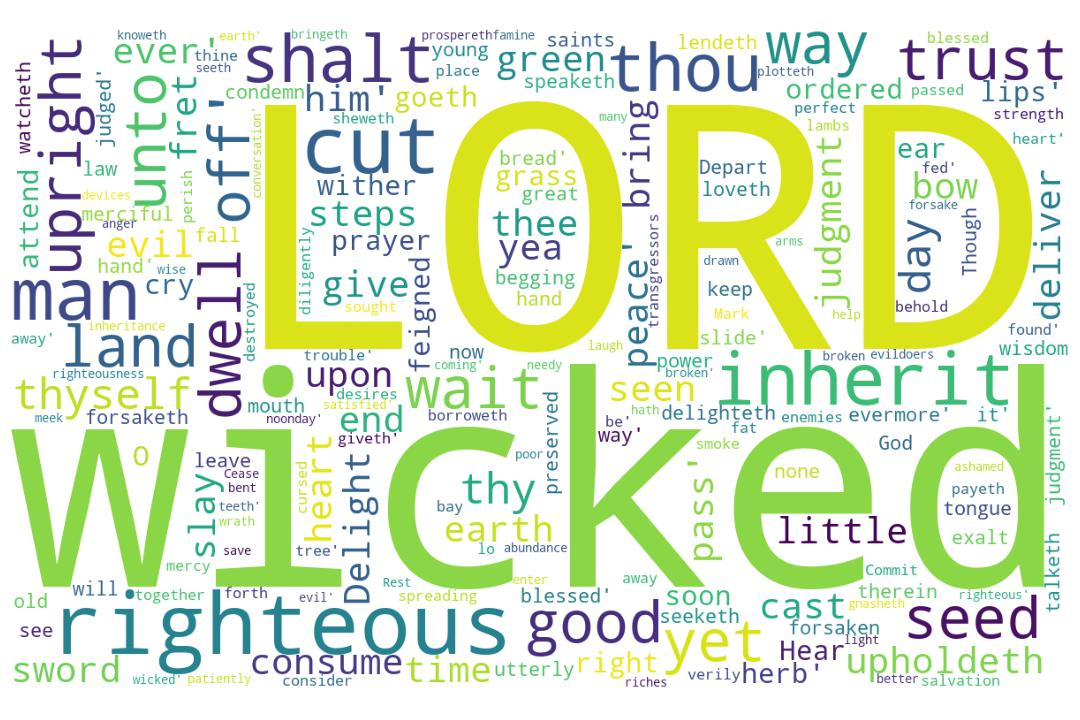
\includegraphics[width=\linewidth]{19OT-Psalms/Psalm37-WordCloud.jpg}
  \caption{Psalm 37 Word Cloud}
  \label{fig:Psalm 37  word Cloud}
\end{figure}

\marginpar{\scriptsize \centering \fcolorbox{bone}{lime}{\textbf{TEMPORARY TRIUMPH}}\\ (Psalm 37:1-40) \begin{compactenum}[I.][14]
   \item An \textbf{Apparent Problem} \index[scripture]{Psalms!Psa 037:01}(Psa 37:1) 
   \item An \textbf{Abundant Peace} \index[scripture]{Psalms!Psa 037:11}(Psa 37:11) 
   \item The \textbf{Aweful Potting} \index[scripture]{Psalms!Psa 037:12}(Psa 37:12) 
   \item The \textbf{Anticipated Perishing} \index[scripture]{Psalms!Psa 037:20}(Psa 37:20) 
    \item \textbf{Almighty Preservation} \index[scripture]{Psalms!Psa 037:28}(Psa 37:28)
    \item Their \textbf{Apparent Power} \index[scripture]{Psalms!Psa 037:35}(Psa 37:35)
    \item An \textbf{Awaited Passing} \index[scripture]{Psalms!Psa 037:36}(Psa 37:36)
    \item \textbf{Abandoned Paths} \index[scripture]{Psalms!Psa 037:01-11}(Psa 37:1--11)
    \item \textbf{Awesome Prophecies} \index[scripture]{Psalms!Psa 037:01-40}(Psa 37:1--40)
    \item \textbf{Attractive Pursuits} \index[scripture]{Psalms!Psa 037:11-22}(Psa 37:11--22)
    \item \textbf{Abiding Principles} \index[scripture]{Psalms!Psa 037:32-40}(Psa 37:32--40)
    \item \textbf{Absolute Promises} \index[scripture]{Psalms!Psa 037:01-11}(Psa 37:1--11)
\end{compactenum}}

\footnote{\textcolor[cmyk]{0.99998,1,0,0}{\hyperlink{TOC}{Return to end of Table of Contents.}}}\footnote{\href{https://audiobible.com/bible}{\textcolor[cmyk]{0.99998,1,0,0}{Psalm 37 Audio}}}\textcolor[cmyk]{0.99998,1,0,0}{\emph{A Psalm} of David.}\\
\\
\textcolor[cmyk]{0.99998,1,0,0}{Fret \fcolorbox{bone}{bone}{not} thyself because of \fcolorbox{bone}{lime}{evildoers}, neither be thou envious against the workers of iniquity.}
[2] \textcolor[cmyk]{0.99998,1,0,0}{For they shall soon be cut down like the grass, and wither as the green herb.}
[3] \textcolor[cmyk]{0.99998,1,0,0}{Trust in \fcolorbox{bone}{bone}{the LORD}, and do good; \emph{so} shalt thou dwell in the land, and verily thou shalt be fed.}
[4] \textcolor[cmyk]{0.99998,1,0,0}{Delight thyself also in \fcolorbox{bone}{bone}{the LORD}; and \fcolorbox{bone}{bone}{he} shall give thee the desires of thine heart.}
[5] \textcolor[cmyk]{0.99998,1,0,0}{Commit thy way unto \fcolorbox{bone}{bone}{the LORD}; trust also in him; and \fcolorbox{bone}{bone}{he} shall bring \emph{it} to pass.}
[6] \textcolor[cmyk]{0.99998,1,0,0}{And \fcolorbox{bone}{bone}{he} shall bring forth thy righteousness as the light, and thy judgment as the noonday.}
[7] \textcolor[cmyk]{0.99998,1,0,0}{Rest in \fcolorbox{bone}{bone}{the LORD}, and wait patiently for him: fret \fcolorbox{bone}{bone}{not} thyself because of him who prospereth in his way, because of the man who bringeth wicked devices to pass.}
[8] \textcolor[cmyk]{0.99998,1,0,0}{Cease from anger, and forsake wrath: fret \fcolorbox{bone}{bone}{not} thyself in any wise to do evil.}
[9] \textcolor[cmyk]{0.99998,1,0,0}{For evildoers shall be cut off: but those that wait upon \fcolorbox{bone}{bone}{the LORD}, they shall inherit the earth.}
[10] \textcolor[cmyk]{0.99998,1,0,0}{For yet a little while, and the wicked \emph{shall} \fcolorbox{bone}{bone}{not} \emph{be}: yea, thou shalt diligently consider his place, and it \emph{shall} \fcolorbox{bone}{bone}{not} \emph{be}.}
[11] \textcolor[cmyk]{0.99998,1,0,0}{But the meek shall inherit the earth; and shall delight themselves in the abundance of \fcolorbox{bone}{lime}{peace}.}\footnote{\textbf{Matthew 5;5} - Blessed are the meek: for they shall inherit the earth.}
[12] \textcolor[cmyk]{0.99998,1,0,0}{The wicked \fcolorbox{bone}{lime}{plotteth} against the just, and gnasheth upon him with his teeth.}
[13] \textcolor[cmyk]{0.99998,1,0,0}{The Lord shall laugh at him: for \fcolorbox{bone}{bone}{he} seeth that his day is coming.}
[14] \textcolor[cmyk]{0.99998,1,0,0}{The wicked have drawn out the sword, and have bent their bow, to cast down the poor and needy, \emph{and} to slay such as be of upright conversation.}
[15] \textcolor[cmyk]{0.99998,1,0,0}{Their sword shall enter into their own heart, and their bows shall be broken.}
[16] \textcolor[cmyk]{0.99998,1,0,0}{A little that a righteous man hath \emph{is} better than the riches of many wicked.}
[17] \textcolor[cmyk]{0.99998,1,0,0}{For the arms of the wicked shall be broken: but \fcolorbox{bone}{bone}{the LORD} upholdeth the righteous.}
[18] \textcolor[cmyk]{0.99998,1,0,0}{The LORD knoweth the days of the upright: and their inheritance shall be for ever.}
[19] \textcolor[cmyk]{0.99998,1,0,0}{They shall \fcolorbox{bone}{bone}{not} be ashamed in the evil time: and in the days of famine they shall be satisfied.}
[20] \textcolor[cmyk]{0.99998,1,0,0}{But the wicked shall \fcolorbox{bone}{lime}{perish}, and the enemies of \fcolorbox{bone}{bone}{the LORD} \emph{shall} \emph{be} as the fat of lambs: they shall consume; into smoke shall they consume away.}
[21] \textcolor[cmyk]{0.99998,1,0,0}{The wicked borroweth, and payeth \fcolorbox{bone}{bone}{not} again: but the righteous sheweth mercy, and giveth.}
[22] \textcolor[cmyk]{0.99998,1,0,0}{For \emph{such} \emph{as} \emph{be} blessed of him shall inherit the earth; and \emph{they} \emph{that} \emph{be} cursed of him shall be cut off.}
[23] \textcolor[cmyk]{0.99998,1,0,0}{The steps of a \emph{good} man are ordered by \fcolorbox{bone}{bone}{the LORD}: and \fcolorbox{bone}{bone}{he} delighteth in his way.}
[24] \textcolor[cmyk]{0.99998,1,0,0}{Though \fcolorbox{bone}{bone}{he} fall, \fcolorbox{bone}{bone}{he} shall \fcolorbox{bone}{bone}{not} be utterly cast down: for \fcolorbox{bone}{bone}{the LORD} upholdeth \emph{him} \emph{with} his hand.}
[25] \textcolor[cmyk]{0.99998,1,0,0}{I have been young, and \emph{now} am old; yet have I \fcolorbox{bone}{bone}{not} seen the righteous forsaken, nor his seed begging bread.}
[26] \textcolor[cmyk]{0.99998,1,0,0}{He \emph{is} ever merciful, and lendeth; and his seed \emph{is} blessed.}
[27] \textcolor[cmyk]{0.99998,1,0,0}{Depart from evil, and do good; and dwell for evermore.}
[28] \textcolor[cmyk]{0.99998,1,0,0}{For \fcolorbox{bone}{bone}{the LORD} loveth judgment, and forsaketh \fcolorbox{bone}{bone}{not} his saints; they are \fcolorbox{bone}{lime}{preserved} for ever: but the seed of the wicked shall be cut off.}
[29] \textcolor[cmyk]{0.99998,1,0,0}{The righteous shall inherit the land, and dwell therein for ever.}
[30] \textcolor[cmyk]{0.99998,1,0,0}{The mouth of the righteous speaketh wisdom, and his tongue talketh of judgment.}
[31] \textcolor[cmyk]{0.99998,1,0,0}{The law of his God \emph{is} in his heart; none of his steps shall slide.}
[32] \textcolor[cmyk]{0.99998,1,0,0}{The wicked watcheth the righteous, and seeketh to slay him.}
[33] \textcolor[cmyk]{0.99998,1,0,0}{The LORD will \fcolorbox{bone}{bone}{not} leave him in his hand, nor condemn him when \fcolorbox{bone}{bone}{he} is judged.}
[34] \textcolor[cmyk]{0.99998,1,0,0}{Wait on \fcolorbox{bone}{bone}{the LORD}, and keep his way, and \fcolorbox{bone}{bone}{he} shall exalt thee to inherit the land: when the wicked are cut off, thou shalt see \emph{it}.}
[35] \textcolor[cmyk]{0.99998,1,0,0}{I have seen the wicked in great \fcolorbox{bone}{lime}{power}, and spreading himself like a green bay tree.}\footnote{\textbf{Matthew 13:31-32} - Another parable put he forth unto them, saying, The kingdom of heaven is like to a grain of mustard seed, which a man took, and sowed in his field: [32 ]Which indeed is the least of all seeds: but when it is grown, it is the greatest among herbs, and becometh a tree, so that the birds of the air come and lodge in the branches thereof.}
[36] \textcolor[cmyk]{0.99998,1,0,0}{Yet \fcolorbox{bone}{bone}{he} \fcolorbox{bone}{lime}{passed} away, and, lo, \fcolorbox{bone}{bone}{he} \emph{was} \fcolorbox{bone}{bone}{not}: yea, I sought him, but \fcolorbox{bone}{bone}{he} could \fcolorbox{bone}{bone}{not} be found.}
[37] \textcolor[cmyk]{0.99998,1,0,0}{Mark the perfect \emph{man}, and behold the upright: for the end of \emph{that} man \emph{is} peace.}
[38] \textcolor[cmyk]{0.99998,1,0,0}{But the transgressors shall be destroyed together: the end of the wicked shall be cut off.}
[39] \textcolor[cmyk]{0.99998,1,0,0}{But the salvation of the righteous \emph{is} of \fcolorbox{bone}{bone}{the LORD}: \emph{he} \emph{is} their strength in the time of trouble.}\footnote{\textbf{Job 38:23} - Which I have reserved against the time of trouble, against the day of battle and war?}\footnote{\textbf{Psalm 27:15} - For in the time of trouble he shall hide me in his pavilion: in the secret of his tabernacle shall he hide me; he shall set me up upon a rock.}\footnote{\textbf{Psalm 41:1} - Blessed is he that considereth the poor: the LORD will deliver him in time of trouble.}\footnote{\textbf{Proverb 25:19} - Confidence in an unfaithful man in time of trouble is like a broken tooth, and a foot out of joint.}\footnote{\textbf{Isaiah 33:2} -O LORD, be gracious unto us; we have waited for thee: be thou their arm every morning, our salvation also in the time of trouble.}\footnote{\textbf{Jeremiah 14:18} - O the hope of Israel, the saviour thereof in time of trouble, why shouldest thou be as a stranger in the land, and as a wayfaring man that turneth aside to tarry for a night?}\footnote{\textbf{Daniel 12:1} - And at that time shall Michael stand up, the great prince which standeth for the children of thy people: and there shall be a time of trouble, such as never was since there was a nation even to that same time: and at that time thy people shall be delivered, every one that shall be found written in the book.}
[40] \textcolor[cmyk]{0.99998,1,0,0}{And \fcolorbox{bone}{bone}{the LORD} shall help them, and deliver them: \fcolorbox{bone}{bone}{he} shall deliver them from the wicked, and save them, because they trust in him.}




\section{Psalm 37 Comments}

\subsection{Numeric Nuggets}
\textbf{13: } the words ``not'' and ``he'' are used 13 times in the chapter. The phrase ``the LORD'' is used 13 times in the chapter.
%\input{19OT-Psalms/Psalm37-WordIndex}
\section{Psalm 37 Outlines}

\subsection{My Outlines}

\subsubsection{Looking Back}
\index[speaker]{Keith Anthony!Psalm 037:25 (Looking Back)}
\index[series]{Psalms (Keith Anthony)!Psalm 037:25 (Looking Back)}
\index[date]{2016/10/09!Psalm 037:25 (Looking Back) (Keith Anthony)}
\textbf{Introduction: }This past week, I've watched someone pass a significant age milestone, but it is one I passed quite a while ago.  I have always liked Psalm 37, but especially verse 25\index[scripture]{Psalms!Psa 037:25}. The verse talks about some inevitable things, like getting old.  And, it talks about some certain things for a Christian, such as God never forsaking his people and always providing for them. I have seen this in my 38 years of being a Christian, and I've seen other things. So, this is a short commentary on my first 38 years of Christianity. \footnote{09 October 2016, Keith Anthony}
\begin{compactenum}[I.][19]
    \item A \textbf{Slow Burn.} \index[scripture]{Hebrews!Heb 12:01}(Hebrews 12:1) I see this in at least two ways.  First there is the long \textbf{race}, a marathon, for believers. Christianity is not a print: it is a distance event. Christianity is a tedious and day-by-day journey. The second aspect is that of \textbf{refining}. I am thankful that the refining in my life, a necessary thing, has been a slow burn. Look at Psa 12:6-7. Like the completion of a perfect Bible, refining uses fire and heat to burn out impurities and imperfections. I don't like pain. I don't like trouble. I don't like trials. I really don't even like heat and fire.  I don't like getting burned! Maybe a slow and steady refinement is a good thing. 
    \item \textbf{Speed Bumps.} Another thing I've encountered along my Christian experience is speed bumps.  These have been times when big events or situations have knocked my off the slow and steady, maybe even predictable, path. It is especially important to note that many, if not all, of these have been of my OWN doing.  It may be a scandalous thing, but God has gotten me through each of these. %\index[scripture]{Hebrews!Hebrews 12:01}(Hebrews 12:1) 
    \item All \textbf{Sorts of Brethren.} Another part of Christianity has been the fact that God has brought all sorts of brethren into my life. Some have passed.  Some are close at hand. All, though, have made part of my life for a specific reason. Some I have helped. Many more have helped me. Some ... I don't know yet! For some, the next time I see them will be in heaven where for eternity we can talk of God's goodness. %\index[scripture]{Hebrews!Hebrews 12:01}(Hebrews 12:1
    \item A \textbf{Special Book.} One thing that has motivated my Christianity has been the Bible.  I for one cannot understand any Christian who does not have a burning and consuming passion to understand every word in it.  What does one actually do with a perfect and living book? Open it up once or twice a week? Ignore it when it is inconvenient? Its a whole new ball game when you recognize the Bible for what it is .... %\index[scripture]{Hebrews!Hebrews 12:01}(Hebrews 12:1) 
    \item A \textbf{Solid Beliefs.} God gives us solid, consistent, and reliable body of beliefs and then He proves them over and over again.  Beliefs such as saved by grace alone, belief that all things work together for good to those who love God, belief that God's word will not return void!%\index[scripture]{Hebrews!Hebrews 12:01}(Hebrews 12:1) 
    \item \textbf{Special Blessings.} God graces us with special blessings. How about time I got to lead my son to the Lord? What about my grandchildren? What about God providing direction in life and leading to a church where scripture is magnified?  %\index[scripture]{Hebrews!Hebrews 12:01}(Hebrews 12:1)
    %\item A \textbf{Splendid Bride.} 
    \item A \textbf{School Building.} So salvation is just the beginning.  The rest of Christian life is getting to know God, getting to know truth, getting to learn how to be blessing to God and his people. %\index[scripture]{Hebrews!Hebrews 12:01}(Hebrews 12:1)
    \item (Looking Ahead) A \textbf{Spectacular Baccalaureate (Graduation).} Finally, I have something quite unique to look forward to and that is what comes after this life. Turn to 1 Corinthians 2:9. Now think of the best thing that has happened to you in this life.  It will be incomparable to what awaits the believer. %\index[scripture]{Hebrews!Hebrews 12:01}(Hebrews 12:1) 
\end{compactenum}


\subsubsection{Temporary Triumph}

\index[speaker]{Keith Anthony!Psalm 037 (Temporary Triumph)}
\index[series]{Psalms (Keith Anthony)!Psalm 037 (Temporary Triumph)}
\index[date]{2016/07/13!Psalm 037 (Temporary Triumph) (Keith Anthony)}

\begin{compactenum}[I.][19]
   \item An \textbf{Apparent Problem} \index[scripture]{Psalms!Psa 037:01}(Psa 37:1) 
   \item An \textbf{Abundant Peace} \index[scripture]{Psalms!Psa 037:11}(Psa 37:11) 
   \item The \textbf{Aweful Potting} \index[scripture]{Psalms!Psa 037:12}(Psa 37:12) 
   \item The \textbf{Anticipated Perishing} \index[scripture]{Psalms!Psa 037:20}(Psa 37:20) 
    \item \textbf{Almighty Preservation} \index[scripture]{Psalms!Psa 037:28}(Psa 37:28)
 \item Their \textbf{Apparent Power} \index[scripture]{Psalms!Psa 037:35}(Psa 37:35)
 \item An \textbf{Awaited Passing} \index[scripture]{Psalms!Psa 037:36}(Psa 37:36)
\end{compactenum}






\subsection{Outlines from Others}





%\section{Psalm 37 Statistics}

%%%%%%%%%%%%%%%%%%%%%%%%%%%
%%%%% Word Statistics
%%%%%%%%%%%%%%%%%%%%%%%%%%


\normalsize



\subsection{Chapter Word Statistics}


%%%%%%%%%%
%%%%%%%%%%
 
\begin{center}
\begin{longtable}{l|c|c|c|c}
\caption[Stats for Psalm 37]{Stats for Psalm 37} \label{table:Stats for Psalm 37} \\ 
\hline \multicolumn{1}{|c|}{\textbf{Verse(s)}} & \multicolumn{1}{|c|}{\textbf{Count}} & \multicolumn{1}{|c|}{\textbf{Unique}} & \multicolumn{1}{|c|}{\textbf{Italics}} & \multicolumn{1}{|c|}{\textbf{Uniq Italic}}  \\ \hline 
\endfirsthead
 
\multicolumn{5}{c}
{{\bfseries \tablename\ \thetable{} -- continued from previous page}} \\  
\hline \multicolumn{1}{|c|}{\textbf{Verse(s)}} & \multicolumn{1}{|c|}{\textbf{Count}} & \multicolumn{1}{|c|}{\textbf{Unique}} & \multicolumn{1}{|c|}{\textbf{Italics}} & \multicolumn{1}{|c|}{\textbf{Uniq Italic}}  \\ \hline 
\endhead
 
\hline \multicolumn{5}{|r|}{{Continued if needed}} \\ \hline
\endfoot 
1 & 15 & 14 & 0 & 0\\ \hline
2 & 16 & 15 & 0 & 0\\ \hline
3 & 20 & 15 & 1 & 1\\ \hline
4 & 16 & 15 & 0 & 0\\ \hline
5 & 17 & 17 & 1 & 1\\ \hline
6 & 16 & 13 & 0 & 0\\ \hline
7 & 30 & 24 & 0 & 0\\ \hline
8 & 15 & 15 & 0 & 0\\ \hline
9 & 18 & 16 & 0 & 0\\ \hline
10 & 23 & 19 & 4 & 2\\ \hline
11 & 16 & 13 & 0 & 0\\ \hline
12 & 13 & 13 & 0 & 0\\ \hline
13 & 14 & 14 & 0 & 0\\ \hline
14 & 28 & 24 & 1 & 1\\ \hline
15 & 14 & 12 & 0 & 0\\ \hline
16 & 15 & 15 & 1 & 1\\ \hline
17 & 15 & 12 & 0 & 0\\ \hline
18 & 15 & 14 & 0 & 0\\ \hline
19 & 19 & 15 & 0 & 0\\ \hline
20 & 27 & 19 & 2 & 2\\ \hline
21 & 14 & 13 & 0 & 0\\ \hline
22 & 22 & 18 & 6 & 5\\ \hline
23 & 17 & 17 & 1 & 1\\ \hline
24 & 18 & 17 & 2 & 2\\ \hline
25 & 21 & 19 & 1 & 1\\ \hline
26 & 11 & 9 & 3 & 2\\ \hline
27 & 10 & 9 & 0 & 0\\ \hline
28 & 25 & 23 & 0 & 0\\ \hline
29 & 11 & 11 & 0 & 0\\ \hline
30 & 13 & 12 & 0 & 0\\ \hline
31 & 15 & 12 & 1 & 1\\ \hline
32 & 10 & 10 & 0 & 0\\ \hline
33 & 16 & 15 & 0 & 0\\ \hline
34 & 27 & 24 & 1 & 1\\ \hline
35 & 16 & 16 & 0 & 0\\ \hline
36 & 19 & 16 & 1 & 1\\ \hline
37 & 16 & 14 & 3 & 3\\ \hline
38 & 16 & 12 & 0 & 0\\ \hline
39 & 19 & 13 & 3 & 2\\ \hline
40 & 24 & 17 & 0 & 0\\ \hline
\hline \hline
Total & 702 & 262 & 32 & 18



\end{longtable}
\end{center}

%%%%%%%%%%
%%%%%%%%%%
 
\subsection{Words by Frequency}

\begin{center}
\begin{longtable}{l|r}
\caption[Word Frequencies in Psalm 37]{Word Frequencies in Psalm 37} \label{table:WordsIn-Psalm-37} \\ 
\hline \multicolumn{1}{|c|}{\textbf{Word}} & \multicolumn{1}{c|}{\textbf{Frequency}} \\ \hline 
\endfirsthead
 
\multicolumn{2}{c}
{{\bfseries \tablename\ \thetable{} -- continued from previous page}} \\ 
\hline \multicolumn{1}{|c|}{\textbf{Word}} & \multicolumn{1}{c|}{\textbf{Frequency}} \\ \hline 
\endhead
 
\hline \multicolumn{2}{|r|}{{Continued if needed}} \\ \hline
\endfoot
 
\hline \hline
\endlastfoot
the & 61 \\ \hline
and & 38 \\ \hline
shall & 29 \\ \hline
of & 26 \\ \hline
be & 16 \\ \hline
in & 16 \\ \hline
LORD & 15 \\ \hline
his & 15 \\ \hline
wicked & 14 \\ \hline
not & 13 \\ \hline
he & 13 \\ \hline
him & 12 \\ \hline
The & 11 \\ \hline
for & 8 \\ \hline
righteous & 8 \\ \hline
they & 7 \\ \hline
to & 7 \\ \hline
\emph{is} & 7 \\ \hline
For & 6 \\ \hline
cut & 6 \\ \hline
thou & 5 \\ \hline
as & 5 \\ \hline
off & 5 \\ \hline
but & 5 \\ \hline
inherit & 5 \\ \hline
\emph{be} & 5 \\ \hline
have & 5 \\ \hline
their & 5 \\ \hline
thyself & 4 \\ \hline
because & 4 \\ \hline
shalt & 4 \\ \hline
way & 4 \\ \hline
man & 4 \\ \hline
a & 4 \\ \hline
But & 4 \\ \hline
ever & 4 \\ \hline
I & 4 \\ \hline
them & 4 \\ \hline
down & 3 \\ \hline
do & 3 \\ \hline
dwell & 3 \\ \hline
land & 3 \\ \hline
heart & 3 \\ \hline
thy & 3 \\ \hline
judgment & 3 \\ \hline
from & 3 \\ \hline
evil & 3 \\ \hline
that & 3 \\ \hline
earth & 3 \\ \hline
\emph{shall} & 3 \\ \hline
upright & 3 \\ \hline
are & 3 \\ \hline
seed & 3 \\ \hline
evildoers & 2 \\ \hline
against & 2 \\ \hline
like & 2 \\ \hline
green & 2 \\ \hline
good & 2 \\ \hline
also & 2 \\ \hline
thee & 2 \\ \hline
trust & 2 \\ \hline
bring & 2 \\ \hline
\emph{it} & 2 \\ \hline
pass & 2 \\ \hline
And & 2 \\ \hline
wait & 2 \\ \hline
fret & 2 \\ \hline
who & 2 \\ \hline
upon & 2 \\ \hline
yet & 2 \\ \hline
little & 2 \\ \hline
yea & 2 \\ \hline
peace & 2 \\ \hline
is & 2 \\ \hline
sword & 2 \\ \hline
cast & 2 \\ \hline
slay & 2 \\ \hline
into & 2 \\ \hline
broken & 2 \\ \hline
upholdeth & 2 \\ \hline
days & 2 \\ \hline
time & 2 \\ \hline
consume & 2 \\ \hline
away & 2 \\ \hline
blessed & 2 \\ \hline
\emph{that} & 2 \\ \hline
steps & 2 \\ \hline
hand & 2 \\ \hline
seen & 2 \\ \hline
nor & 2 \\ \hline
when & 2 \\ \hline
end & 2 \\ \hline
deliver & 2 \\ \hline
Fret & 1 \\ \hline
neither & 1 \\ \hline
envious & 1 \\ \hline
workers & 1 \\ \hline
iniquity & 1 \\ \hline
soon & 1 \\ \hline
grass & 1 \\ \hline
wither & 1 \\ \hline
herb & 1 \\ \hline
Trust & 1 \\ \hline
\emph{so} & 1 \\ \hline
verily & 1 \\ \hline
fed & 1 \\ \hline
Delight & 1 \\ \hline
give & 1 \\ \hline
desires & 1 \\ \hline
thine & 1 \\ \hline
Commit & 1 \\ \hline
unto & 1 \\ \hline
forth & 1 \\ \hline
righteousness & 1 \\ \hline
light & 1 \\ \hline
noonday & 1 \\ \hline
Rest & 1 \\ \hline
patiently & 1 \\ \hline
prospereth & 1 \\ \hline
bringeth & 1 \\ \hline
devices & 1 \\ \hline
Cease & 1 \\ \hline
anger & 1 \\ \hline
forsake & 1 \\ \hline
wrath & 1 \\ \hline
any & 1 \\ \hline
wise & 1 \\ \hline
those & 1 \\ \hline
while & 1 \\ \hline
diligently & 1 \\ \hline
consider & 1 \\ \hline
place & 1 \\ \hline
it & 1 \\ \hline
meek & 1 \\ \hline
delight & 1 \\ \hline
themselves & 1 \\ \hline
abundance & 1 \\ \hline
plotteth & 1 \\ \hline
just & 1 \\ \hline
gnasheth & 1 \\ \hline
with & 1 \\ \hline
teeth & 1 \\ \hline
Lord & 1 \\ \hline
laugh & 1 \\ \hline
at & 1 \\ \hline
seeth & 1 \\ \hline
day & 1 \\ \hline
coming & 1 \\ \hline
drawn & 1 \\ \hline
out & 1 \\ \hline
bent & 1 \\ \hline
bow & 1 \\ \hline
poor & 1 \\ \hline
needy & 1 \\ \hline
\emph{and} & 1 \\ \hline
such & 1 \\ \hline
conversation & 1 \\ \hline
Their & 1 \\ \hline
enter & 1 \\ \hline
own & 1 \\ \hline
bows & 1 \\ \hline
A & 1 \\ \hline
hath & 1 \\ \hline
better & 1 \\ \hline
than & 1 \\ \hline
riches & 1 \\ \hline
many & 1 \\ \hline
arms & 1 \\ \hline
knoweth & 1 \\ \hline
inheritance & 1 \\ \hline
They & 1 \\ \hline
ashamed & 1 \\ \hline
famine & 1 \\ \hline
satisfied & 1 \\ \hline
perish & 1 \\ \hline
enemies & 1 \\ \hline
fat & 1 \\ \hline
lambs & 1 \\ \hline
smoke & 1 \\ \hline
borroweth & 1 \\ \hline
payeth & 1 \\ \hline
again & 1 \\ \hline
sheweth & 1 \\ \hline
mercy & 1 \\ \hline
giveth & 1 \\ \hline
\emph{such} & 1 \\ \hline
\emph{as} & 1 \\ \hline
\emph{they} & 1 \\ \hline
cursed & 1 \\ \hline
\emph{good} & 1 \\ \hline
ordered & 1 \\ \hline
by & 1 \\ \hline
delighteth & 1 \\ \hline
Though & 1 \\ \hline
fall & 1 \\ \hline
utterly & 1 \\ \hline
\emph{him} & 1 \\ \hline
\emph{with} & 1 \\ \hline
been & 1 \\ \hline
young & 1 \\ \hline
\emph{now} & 1 \\ \hline
am & 1 \\ \hline
old & 1 \\ \hline
forsaken & 1 \\ \hline
begging & 1 \\ \hline
bread & 1 \\ \hline
\emph{He} & 1 \\ \hline
merciful & 1 \\ \hline
lendeth & 1 \\ \hline
Depart & 1 \\ \hline
evermore & 1 \\ \hline
loveth & 1 \\ \hline
forsaketh & 1 \\ \hline
saints & 1 \\ \hline
preserved & 1 \\ \hline
therein & 1 \\ \hline
mouth & 1 \\ \hline
speaketh & 1 \\ \hline
wisdom & 1 \\ \hline
tongue & 1 \\ \hline
talketh & 1 \\ \hline
law & 1 \\ \hline
God & 1 \\ \hline
none & 1 \\ \hline
slide & 1 \\ \hline
watcheth & 1 \\ \hline
seeketh & 1 \\ \hline
will & 1 \\ \hline
leave & 1 \\ \hline
condemn & 1 \\ \hline
judged & 1 \\ \hline
Wait & 1 \\ \hline
on & 1 \\ \hline
keep & 1 \\ \hline
exalt & 1 \\ \hline
see & 1 \\ \hline
great & 1 \\ \hline
power & 1 \\ \hline
spreading & 1 \\ \hline
himself & 1 \\ \hline
bay & 1 \\ \hline
tree & 1 \\ \hline
Yet & 1 \\ \hline
passed & 1 \\ \hline
lo & 1 \\ \hline
\emph{was} & 1 \\ \hline
sought & 1 \\ \hline
could & 1 \\ \hline
found & 1 \\ \hline
Mark & 1 \\ \hline
perfect & 1 \\ \hline
\emph{man} & 1 \\ \hline
behold & 1 \\ \hline
transgressors & 1 \\ \hline
destroyed & 1 \\ \hline
together & 1 \\ \hline
salvation & 1 \\ \hline
\emph{he} & 1 \\ \hline
strength & 1 \\ \hline
trouble & 1 \\ \hline
help & 1 \\ \hline
save & 1 \\ \hline
\end{longtable}
\end{center}



\normalsize



\subsection{Words Alphabetically}

\begin{center}
\begin{longtable}{l|r}
\caption[Word Alphabetically in Psalm 37]{Word Alphabetically in Psalm 37} \label{table:WordsIn-Psalm-37} \\ 
\hline \multicolumn{1}{|c|}{\textbf{Word}} & \multicolumn{1}{c|}{\textbf{Frequency}} \\ \hline 
\endfirsthead
 
\multicolumn{2}{c}
{{\bfseries \tablename\ \thetable{} -- continued from previous page}} \\ 
\hline \multicolumn{1}{|c|}{\textbf{Word}} & \multicolumn{1}{c|}{\textbf{Frequency}} \\ \hline 
\endhead
 
\hline \multicolumn{2}{|r|}{{Continued if needed}} \\ \hline
\endfoot
 
\hline \hline
\endlastfoot
A & 1 \\ \hline
And & 2 \\ \hline
But & 4 \\ \hline
Cease & 1 \\ \hline
Commit & 1 \\ \hline
Delight & 1 \\ \hline
Depart & 1 \\ \hline
For & 6 \\ \hline
Fret & 1 \\ \hline
God & 1 \\ \hline
I & 4 \\ \hline
LORD & 15 \\ \hline
Lord & 1 \\ \hline
Mark & 1 \\ \hline
Rest & 1 \\ \hline
The & 11 \\ \hline
Their & 1 \\ \hline
They & 1 \\ \hline
Though & 1 \\ \hline
Trust & 1 \\ \hline
Wait & 1 \\ \hline
Yet & 1 \\ \hline
\emph{He} & 1 \\ \hline
\emph{and} & 1 \\ \hline
\emph{as} & 1 \\ \hline
\emph{be} & 5 \\ \hline
\emph{good} & 1 \\ \hline
\emph{he} & 1 \\ \hline
\emph{him} & 1 \\ \hline
\emph{is} & 7 \\ \hline
\emph{it} & 2 \\ \hline
\emph{man} & 1 \\ \hline
\emph{now} & 1 \\ \hline
\emph{shall} & 3 \\ \hline
\emph{so} & 1 \\ \hline
\emph{such} & 1 \\ \hline
\emph{that} & 2 \\ \hline
\emph{they} & 1 \\ \hline
\emph{was} & 1 \\ \hline
\emph{with} & 1 \\ \hline
a & 4 \\ \hline
abundance & 1 \\ \hline
again & 1 \\ \hline
against & 2 \\ \hline
also & 2 \\ \hline
am & 1 \\ \hline
and & 38 \\ \hline
anger & 1 \\ \hline
any & 1 \\ \hline
are & 3 \\ \hline
arms & 1 \\ \hline
as & 5 \\ \hline
ashamed & 1 \\ \hline
at & 1 \\ \hline
away & 2 \\ \hline
bay & 1 \\ \hline
be & 16 \\ \hline
because & 4 \\ \hline
been & 1 \\ \hline
begging & 1 \\ \hline
behold & 1 \\ \hline
bent & 1 \\ \hline
better & 1 \\ \hline
blessed & 2 \\ \hline
borroweth & 1 \\ \hline
bow & 1 \\ \hline
bows & 1 \\ \hline
bread & 1 \\ \hline
bring & 2 \\ \hline
bringeth & 1 \\ \hline
broken & 2 \\ \hline
but & 5 \\ \hline
by & 1 \\ \hline
cast & 2 \\ \hline
coming & 1 \\ \hline
condemn & 1 \\ \hline
consider & 1 \\ \hline
consume & 2 \\ \hline
conversation & 1 \\ \hline
could & 1 \\ \hline
cursed & 1 \\ \hline
cut & 6 \\ \hline
day & 1 \\ \hline
days & 2 \\ \hline
delight & 1 \\ \hline
delighteth & 1 \\ \hline
deliver & 2 \\ \hline
desires & 1 \\ \hline
destroyed & 1 \\ \hline
devices & 1 \\ \hline
diligently & 1 \\ \hline
do & 3 \\ \hline
down & 3 \\ \hline
drawn & 1 \\ \hline
dwell & 3 \\ \hline
earth & 3 \\ \hline
end & 2 \\ \hline
enemies & 1 \\ \hline
enter & 1 \\ \hline
envious & 1 \\ \hline
ever & 4 \\ \hline
evermore & 1 \\ \hline
evil & 3 \\ \hline
evildoers & 2 \\ \hline
exalt & 1 \\ \hline
fall & 1 \\ \hline
famine & 1 \\ \hline
fat & 1 \\ \hline
fed & 1 \\ \hline
for & 8 \\ \hline
forsake & 1 \\ \hline
forsaken & 1 \\ \hline
forsaketh & 1 \\ \hline
forth & 1 \\ \hline
found & 1 \\ \hline
fret & 2 \\ \hline
from & 3 \\ \hline
give & 1 \\ \hline
giveth & 1 \\ \hline
gnasheth & 1 \\ \hline
good & 2 \\ \hline
grass & 1 \\ \hline
great & 1 \\ \hline
green & 2 \\ \hline
hand & 2 \\ \hline
hath & 1 \\ \hline
have & 5 \\ \hline
he & 13 \\ \hline
heart & 3 \\ \hline
help & 1 \\ \hline
herb & 1 \\ \hline
him & 12 \\ \hline
himself & 1 \\ \hline
his & 15 \\ \hline
in & 16 \\ \hline
inherit & 5 \\ \hline
inheritance & 1 \\ \hline
iniquity & 1 \\ \hline
into & 2 \\ \hline
is & 2 \\ \hline
it & 1 \\ \hline
judged & 1 \\ \hline
judgment & 3 \\ \hline
just & 1 \\ \hline
keep & 1 \\ \hline
knoweth & 1 \\ \hline
lambs & 1 \\ \hline
land & 3 \\ \hline
laugh & 1 \\ \hline
law & 1 \\ \hline
leave & 1 \\ \hline
lendeth & 1 \\ \hline
light & 1 \\ \hline
like & 2 \\ \hline
little & 2 \\ \hline
lo & 1 \\ \hline
loveth & 1 \\ \hline
man & 4 \\ \hline
many & 1 \\ \hline
meek & 1 \\ \hline
merciful & 1 \\ \hline
mercy & 1 \\ \hline
mouth & 1 \\ \hline
needy & 1 \\ \hline
neither & 1 \\ \hline
none & 1 \\ \hline
noonday & 1 \\ \hline
nor & 2 \\ \hline
not & 13 \\ \hline
of & 26 \\ \hline
off & 5 \\ \hline
old & 1 \\ \hline
on & 1 \\ \hline
ordered & 1 \\ \hline
out & 1 \\ \hline
own & 1 \\ \hline
pass & 2 \\ \hline
passed & 1 \\ \hline
patiently & 1 \\ \hline
payeth & 1 \\ \hline
peace & 2 \\ \hline
perfect & 1 \\ \hline
perish & 1 \\ \hline
place & 1 \\ \hline
plotteth & 1 \\ \hline
poor & 1 \\ \hline
power & 1 \\ \hline
preserved & 1 \\ \hline
prospereth & 1 \\ \hline
riches & 1 \\ \hline
righteous & 8 \\ \hline
righteousness & 1 \\ \hline
saints & 1 \\ \hline
salvation & 1 \\ \hline
satisfied & 1 \\ \hline
save & 1 \\ \hline
see & 1 \\ \hline
seed & 3 \\ \hline
seeketh & 1 \\ \hline
seen & 2 \\ \hline
seeth & 1 \\ \hline
shall & 29 \\ \hline
shalt & 4 \\ \hline
sheweth & 1 \\ \hline
slay & 2 \\ \hline
slide & 1 \\ \hline
smoke & 1 \\ \hline
soon & 1 \\ \hline
sought & 1 \\ \hline
speaketh & 1 \\ \hline
spreading & 1 \\ \hline
steps & 2 \\ \hline
strength & 1 \\ \hline
such & 1 \\ \hline
sword & 2 \\ \hline
talketh & 1 \\ \hline
teeth & 1 \\ \hline
than & 1 \\ \hline
that & 3 \\ \hline
the & 61 \\ \hline
thee & 2 \\ \hline
their & 5 \\ \hline
them & 4 \\ \hline
themselves & 1 \\ \hline
therein & 1 \\ \hline
they & 7 \\ \hline
thine & 1 \\ \hline
those & 1 \\ \hline
thou & 5 \\ \hline
thy & 3 \\ \hline
thyself & 4 \\ \hline
time & 2 \\ \hline
to & 7 \\ \hline
together & 1 \\ \hline
tongue & 1 \\ \hline
transgressors & 1 \\ \hline
tree & 1 \\ \hline
trouble & 1 \\ \hline
trust & 2 \\ \hline
unto & 1 \\ \hline
upholdeth & 2 \\ \hline
upon & 2 \\ \hline
upright & 3 \\ \hline
utterly & 1 \\ \hline
verily & 1 \\ \hline
wait & 2 \\ \hline
watcheth & 1 \\ \hline
way & 4 \\ \hline
when & 2 \\ \hline
while & 1 \\ \hline
who & 2 \\ \hline
wicked & 14 \\ \hline
will & 1 \\ \hline
wisdom & 1 \\ \hline
wise & 1 \\ \hline
with & 1 \\ \hline
wither & 1 \\ \hline
workers & 1 \\ \hline
wrath & 1 \\ \hline
yea & 2 \\ \hline
yet & 2 \\ \hline
young & 1 \\ \hline
\end{longtable}
\end{center}



\normalsize



\subsection{Word Lengths in Chapter}
\normalsize
\begin{longtable}{l|p{3.75in}}
\caption[Words by Length in Psalm 37]{Words by Length in Psalm 37} \label{table:WordsIn-Psalm-37} \\ 
\hline \multicolumn{1}{|c|}{\textbf{Length}} & \multicolumn{1}{c|}{\textbf{Words}} \\ \hline 
\endfirsthead
 
\multicolumn{2}{c}
{{\bfseries \tablename\ \thetable{} -- continued from previous page}} \\ 
\hline \multicolumn{1}{|c|}{\textbf{Length}} & \multicolumn{1}{c|}{\textbf{Words}} \\ \hline 
\endhead
 
\hline \multicolumn{2}{|r|}{{Continued if needed}} \\ \hline
\endfoot
 
\hline \hline
\endlastfoot
1 & a, A, I \\ \hline
2 & of, be, as, in, do, \emph{so}, he, \emph{it}, to, \emph{be}, it, at, is, \emph{is}, \emph{as}, by, am, \emph{He}, on, lo, \emph{he} \\ \hline
3 & not, the, For, cut, and, fed, thy, way, him, And, for, who, his, man, any, off, but, yet, yea, But, The, day, out, bow, \emph{and}, own, fat, are, \emph{him}, \emph{now}, old, nor, law, God, see, bay, Yet, \emph{was}, \emph{man}, end \\ \hline
4 & Fret, thou, they, soon, down, like, herb, LORD, good, land, also, give, thee, unto, pass, Rest, wait, fret, from, wise, evil, that, upon, meek, just, with, Lord, have, bent, cast, poor, slay, such, into, bows, hath, than, many, arms, days, ever, They, time, away, \emph{such}, \emph{they}, \emph{that}, \emph{good}, fall, \emph{with}, hand, been, seen, seed, none, will, when, Wait, keep, tree, Mark, help, them, save \\ \hline
5 & shall, grass, green, Trust, shalt, dwell, thine, heart, trust, bring, forth, light, Cease, anger, wrath, those, earth, while, \emph{shall}, place, peace, teeth, laugh, seeth, drawn, sword, their, needy, Their, enter, lambs, smoke, again, mercy, steps, young, bread, mouth, slide, leave, exalt, great, power, could, found \\ \hline
6 & wither, verily, Commit, wicked, little, coming, broken, better, riches, famine, perish, payeth, giveth, cursed, Though, Depart, loveth, saints, wisdom, tongue, judged, passed, sought, behold \\ \hline
7 & thyself, because, neither, envious, against, workers, Delight, desires, noonday, devices, forsake, inherit, delight, upright, knoweth, ashamed, enemies, consume, sheweth, blessed, ordered, utterly, begging, lendeth, therein, talketh, seeketh, condemn, himself, perfect, trouble, deliver \\ \hline
8 & iniquity, judgment, bringeth, consider, plotteth, gnasheth, forsaken, merciful, evermore, speaketh, watcheth, together, strength \\ \hline
9 & evildoers, patiently, abundance, righteous, upholdeth, satisfied, borroweth, forsaketh, preserved, spreading, destroyed, salvation \\ \hline
10 & prospereth, diligently, themselves, delighteth \\ \hline
11 & inheritance \\ \hline
12 & conversation \\ \hline
13 & righteousness, transgressors \\ \hline
\end{longtable}






%%%%%%%%%%
%%%%%%%%%%
 



%%%%%%%%%%
%%%%%%%%%%
\subsection{Verses with 13 Words in Chapter}
\normalsize
\begin{longtable}{l|p{3.75in}}
\caption[Verses with 13 Words  in Psalm 37]{Verses with 13 Words  in Psalm 37} \label{table:Verses with 13 Words in-Psalm-37} \\ 
\hline \multicolumn{1}{|c|}{\textbf{Reference}} & \multicolumn{1}{c|}{\textbf{Verse}} \\ \hline 
\endfirsthead
 
\multicolumn{2}{c}
{{\bfseries \tablename\ \thetable{} -- continued from previous page}} \\ 
\hline \multicolumn{1}{|c|}{\textbf{Reference}} & \multicolumn{1}{c|}{\textbf{Verse}} \\ \hline 
\endhead
 
\hline \multicolumn{2}{|r|}{{Continued if needed}} \\ \hline
\endfoot
 
\hline \hline
\endlastfoot
Psalms 037:12 & The wicked plotteth against the just, and gnasheth upon him with his teeth. \\ \hline
Psalms 037:30 & The mouth of the righteous speaketh wisdom, and his tongue talketh of judgment. \\ \hline
\end{longtable}






%%%%%%%%%%
%%%%%%%%%%
 



%%%%%%%%%%
%%%%%%%%%%
\subsection{Verses with 18 Words in Chapter}
\normalsize
\begin{longtable}{l|p{3.75in}}
\caption[Verses with 18 Words  in Psalm 37]{Verses with 18 Words  in Psalm 37} \label{table:Verses with 18 Words in-Psalm-37} \\ 
\hline \multicolumn{1}{|c|}{\textbf{Reference}} & \multicolumn{1}{c|}{\textbf{Verse}} \\ \hline 
\endfirsthead
 
\multicolumn{2}{c}
{{\bfseries \tablename\ \thetable{} -- continued from previous page}} \\ 
\hline \multicolumn{1}{|c|}{\textbf{Reference}} & \multicolumn{1}{c|}{\textbf{Verse}} \\ \hline 
\endhead
 
\hline \multicolumn{2}{|r|}{{Continued if needed}} \\ \hline
\endfoot
 
\hline \hline
\endlastfoot
Psalms 037:9 & For evildoers shall be cut off: but those that wait upon the LORD, they shall inherit the earth. \\ \hline
Psalms 037:24 & Though he fall, he shall not be utterly cast down: for the LORD upholdeth \emph{him} \emph{with} his hand. \\ \hline
\end{longtable}






%%%%%%%%%%
%%%%%%%%%%
\subsection{Psalm 37 Repeated Phrases}


%%%%%%%%%%
%%%%%%%%%%
\normalsize
 
\begin{center}
\begin{longtable}{|p{3.0in}|p{0.5in}|}
\caption[Psalm 37 Repeated Phrases]{Psalm 37 Repeated Phrases}\label{table:Repeated Phrases Psalm 37} \\
\hline \multicolumn{1}{|c|}{\textbf{Phrase}} & \multicolumn{1}{c|}{\textbf{Frequency}} \\ \hline 
\endfirsthead
 
\multicolumn{2}{c}
{{\bfseries \tablename\ \thetable{} -- continued from previous page}} \\  
\hline \multicolumn{1}{|c|}{\textbf{Phrase}} & \multicolumn{1}{c|}{\textbf{Frequency}} \\ \hline 
\endhead
 
\hline \multicolumn{2}{c}{{ }} \\ \hline
\endfoot 
the LORD & 13\\ \hline 
of the & 9\\ \hline 
shall be & 9\\ \hline 
in the & 8\\ \hline 
the wicked & 8\\ \hline 
he shall & 6\\ \hline 
the righteous & 6\\ \hline 
be cut & 5\\ \hline 
the LORD and & 5\\ \hline 
LORD and & 5\\ \hline 
cut off & 5\\ \hline 
inherit the & 5\\ \hline 
they shall & 4\\ \hline 
as the & 4\\ \hline 
and he & 4\\ \hline 
in his & 4\\ \hline 
shall be cut & 4\\ \hline 
shall be cut off & 4\\ \hline 
be cut off & 4\\ \hline 
shall inherit & 4\\ \hline 
shall inherit the & 4\\ \hline 
But the & 4\\ \hline 
The wicked & 4\\ \hline 
the wicked shall & 4\\ \hline 
wicked shall & 4\\ \hline 
in the LORD & 3\\ \hline 
in the LORD and & 3\\ \hline 
the land & 3\\ \hline 
thou shalt & 3\\ \hline 
and he shall & 3\\ \hline 
of him & 3\\ \hline 
his way & 3\\ \hline 
shall inherit the earth & 3\\ \hline 
inherit the earth & 3\\ \hline 
the earth & 3\\ \hline 
of the wicked & 3\\ \hline 
of the wicked shall & 3\\ \hline 
of the wicked shall be & 3\\ \hline 
the wicked shall be & 3\\ \hline 
wicked shall be & 3\\ \hline 
but the & 3\\ \hline 
for ever & 3\\ \hline 
not be & 3\\ \hline 
\end{longtable}
\end{center}



%%%%%%%%%%
%%%%%%%%%%




\chapter{Psalm 49}

\begin{figure}
  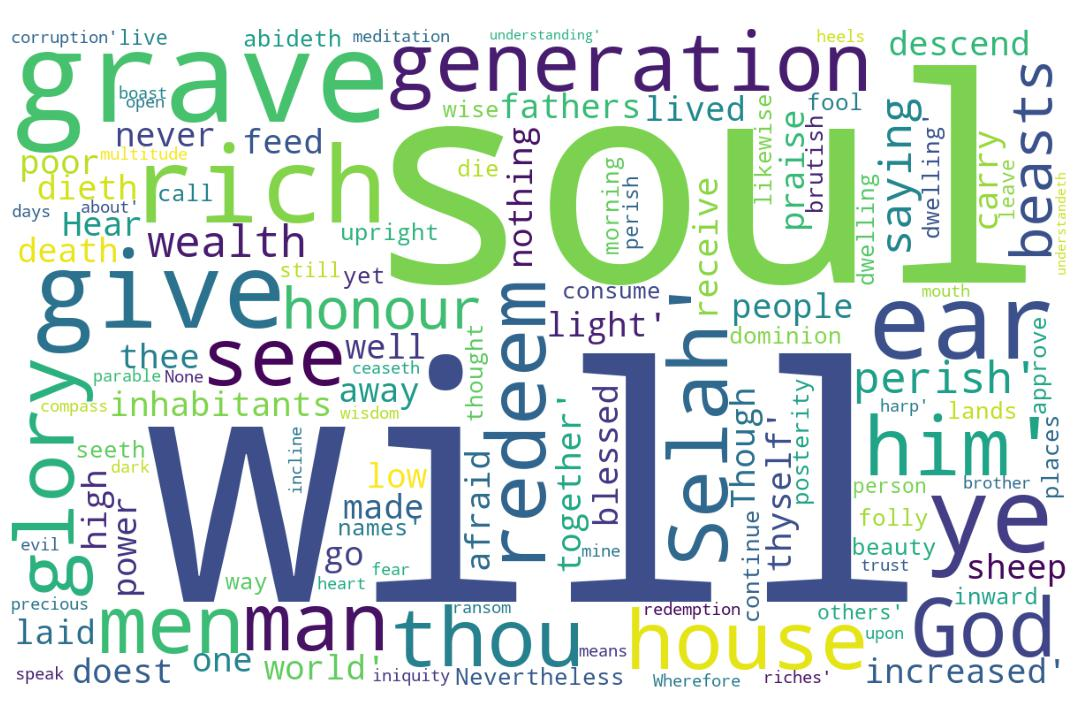
\includegraphics[width=\linewidth]{19OT-Psalms/Psalm49-WordCloud.jpg}
  \caption{Psalm 49 Word Cloud}
  \label{fig:Psalm 49 word Cloud}
\end{figure}

\marginpar{\scriptsize \centering \fcolorbox{bone}{lime}{\textbf{BIG PROBLEMS STILL REMAIN}}\\ (Psalm 49:1-20) \begin{compactenum}[I.][8]
    \item \textbf{Religious Conflict} \index[scripture]{Psalms!Psa 049:13} (Psa 49:13)
    \item \textbf{War} \index[scripture]{Psalms!Psa 049:13} (Psa 49:13)
    \item \textbf{Famine} \index[scripture]{Psalms!Psa 049:13} (Psa 49:13)
    \item \textbf{Sickness} \index[scripture]{Psalms!Psa 049:13} (Psa 49:13)
    \item \textbf{Death} \index[scripture]{Psalms!Psa 049:13} (Psa 49:13)
    \item \textbf{Natural Disasters} \index[scripture]{Psalms!Psa 049:13} (Psa 49:13)
    \item \textbf{Murder and Theft} \index[scripture]{Psalms!Psa 049:13} (Psa 49:13)
\end{compactenum}}


\marginpar{\scriptsize \centering \fcolorbox{bone}{yellow}{\textbf{THE BEASTS THAT PERISH}}\\ (Psalm 49:1-20) \begin{compactenum}[I.][8]
    \item The \textbf{Basic Problems}
    \item The \textbf{Brutish People}
    \item The \textbf{Broken ``Progress''}
    \item The \textbf{Bestowed Possessions}
    \item The \textbf{Beauty that Passes}
    \item The \textbf{Beasts that Perish}
\end{compactenum}}


    
%%%%%%%%%%%%%%%%%%%%%%%%%%%%%%%%%%%%%
%%%%%%%%%%%%%%%%%%%%%%%%%%%%%%%%%%%%%
\footnote{\textcolor[cmyk]{0.99998,1,0,0}{\hyperlink{TOC}{Return to end of Table of Contents.}}}\footnote{\href{https://audiobible.com/bible/psalms_49.html}{\textcolor[cmyk]{0.99998,1,0,0}{Psalms Audio}}}\textcolor[cmyk]{0.99998,1,0,0}{To the chief Musician, A Psalm for the sons of Korah.}\footnote{This is one of the ``orphan'' psalm, with no known author (anonymous), But, it is one of eleven psalms that were for the sons of Korah. (Psalm 42, 44, 45, 46, 47, 48, 49, 84, 85, 87, and 88). The sons of Korah descended from a father who perished under the wrath and curse of God because of his arrogance and pride.   As Korah was a Levite, grandson of Kohath, great-grandson of Levi, this only aggravated his fault, and typifies the sin of Israel, keepers of the oracles of God. \cite{Phillips2001ExploringPsalms1} The count of the psalms for the sons of Korah points to the number 11 as the number of the ``remnant'' as does Hebrews 11 which lists those distinct and select people know for the exercise of faith.}\\
\\
\textcolor[cmyk]{0.99998,1,0,0}{Hear this, all \emph{ye} people; give ear, all \emph{ye} inhabitants of the world:}
[2] \textcolor[cmyk]{0.99998,1,0,0}{Both low and high, rich and poor, together.}
[3] \textcolor[cmyk]{0.99998,1,0,0}{My mouth shall speak of wisdom; and the meditation of my heart \emph{shall} \emph{be} of \fcolorbox{bone}{MYGOLD}{understanding}.}
[4] \textcolor[cmyk]{0.99998,1,0,0}{I will incline mine ear to a parable: I will open my dark saying upon the harp.}
[5] \textcolor[cmyk]{0.99998,1,0,0}{Wherefore should I fear in the days of evil, \emph{when} the iniquity of my heels shall compass me about?}\footnote{The words ``heels'' is found four times in scripture, signifying that someone’s iniquities are following them. What we have done catches up with us (vs. 5). The steps we have stepped, out run us eventually because we step slower and slower. Sooner or later they compass us round about: \cite{Ruckman1992Psalms}
\begin{compactenum}
\item \textbf{Genesis 49:17} -- Dan shall be a serpent by the way, an adder in the path, that biteth the horse heels, so that his rider shall fall backward.
\item \textbf{Job 13:27} -- Thou puttest my feet also in the stocks, and lookest narrowly unto all my paths; thou settest a print upon the heels of my feet.
\item \textbf{Psalm 49:5} -- Wherefore should I fear in the days of evil, \emph{when} the iniquity of my heels shall compass me about?
\item \textbf{Jeremiah 13:22} -- And if thou say in thine heart, Wherefore come these things upon me? For the greatness of thine iniquity are thy skirts discovered, \emph{and} thy heels made bare.
\end{compactenum} }
[6] \textcolor[cmyk]{0.99998,1,0,0}{They that trust in \fcolorbox{bone}{bone}{their} wealth, and boast themselves in the multitude of \fcolorbox{bone}{bone}{their} riches;}\marginpar{\scriptsize \textcolor[rgb]{0.00,0.545,0.269}{$\rightarrow$``Their'' things: 
\begin{compactenum}
	\item their wealth [6, 10],
	\item their riches [6],
	\item their soul [7],
	\item their inward thought [11],
	\item their houses [11],
	\item their dwelling places [11],
	\item their lands [11],
	\item their names [11],
	\item their way [13],
	\item their folly [13],
	\item their posterity [13],
	\item their sayings [13],
	\item their beauty [15], and
	\item dwelling  [15].
\end{compactenum}}}
[7] \textcolor[cmyk]{0.99998,1,0,0}{None \emph{of} \emph{them} can by any means redeem his brother, nor give to God a ransom for him:}
[8] \textcolor[cmyk]{0.99998,1,0,0}{(For the redemption of \fcolorbox{bone}{bone}{their} soul \emph{is} precious, and it ceaseth for ever:)}
[9] \textcolor[cmyk]{0.99998,1,0,0}{That he should still live for ever, \emph{and} not see corruption.}
[10] \textcolor[cmyk]{0.99998,1,0,0}{For he seeth \emph{that} wise men die, likewise the fool and the brutish person perish, and leave \fcolorbox{bone}{bone}{their} wealth to others.}
[11] \textcolor[cmyk]{0.99998,1,0,0}{Their inward thought \emph{is}, \emph{that} \fcolorbox{bone}{bone}{their} houses \emph{shall} \emph{continue} for ever, \emph{and} \fcolorbox{bone}{bone}{their} dwelling places to all generations; they call \emph{their} lands after \fcolorbox{bone}{bone}{their} own names.}
[12] \textcolor[cmyk]{0.99998,1,0,0}{Nevertheless man \emph{being} in honour abideth not: he is like the beasts \emph{that} perish.}
[13] \textcolor[cmyk]{0.99998,1,0,0}{This \fcolorbox{bone}{lime}{\fcolorbox{bone}{bone}{their} way} \emph{is} \fcolorbox{bone}{bone}{their} folly: yet \fcolorbox{bone}{bone}{their} posterity approve \fcolorbox{bone}{bone}{their} sayings. Selah.}
[14] \textcolor[cmyk]{0.99998,1,0,0}{Like sheep they are laid in the grave; death shall feed on them; and the upright shall have dominion over them in the morning; and \fcolorbox{bone}{bone}{their} beauty shall consume in the grave from \fcolorbox{bone}{bone}{their} dwelling.}
[15] \textcolor[cmyk]{0.99998,1,0,0}{But God will redeem my soul from the power of the grave: for he shall receive me. Selah.}
[16] \textcolor[cmyk]{0.99998,1,0,0}{Be not thou afraid when one is made rich, when the glory of his house is increased;}
[17] \textcolor[cmyk]{0.99998,1,0,0}{For when he dieth he shall carry nothing away: his glory shall not descend after him.}
[18] \textcolor[cmyk]{0.99998,1,0,0}{Though while he lived he blessed his soul: and \emph{men} will praise thee, when thou doest well to thyself.}
[19] \textcolor[cmyk]{0.99998,1,0,0}{He shall go to the generation of his fathers; they shall never see light.}
[20] \textcolor[cmyk]{0.99998,1,0,0}{Man \emph{that} \emph{is} in honour, and \fcolorbox{bone}{MYGOLD}{understandeth} not, is like the beasts \emph{that} perish.}
\section{Psalm 49 Comments}

\subsection{Numeric Nuggets}
Verses 1, 8, and 13 have 13 words. Verses 6,  8, 19, and 20 have thirteen unique words. The word ``their'' is used thirteen time in the psalm. (``Their'' is used once, and ``\emph{their}'' is used once.) The 13-letter words ``understanding'' and ``understandeth'' are found in the chapter.

\subsection{Psalm 49:4}
The phrase ``dark saying'', then, is associated with parables. This is the only instance of the phrase, and the phrase ``dark sayings'' is found only twice: \begin{compactenum}
\item \textbf{Psalm 78:2} -- I will open my mouth in a parable: I will utter dark sayings of old: 
\item \textbf{Proverbs 1:6} -- To understand a proverb, and the interpretation; the words of the wise, and their dark sayings.
\end{compactenum}
It is a truth that the ear must be inclined to God to understand a parable before it can be played and sung on a harp. That is why the Psalm was called a ``parable.'' It contains a great deal more than simply warnings against living and dying without redemption or a right relationship to God. The Psalmist is an endtime Jew, when the iniquity of Israel is being paid off double (Isaiah 40:2) for his sin of rejecting the Messiah. The full payment is described in the Lamentations, and the full payment will make Hitler’s holocaust look like exactly what it was: a rehearsal (see Jeremiah 16:16, Amos 9:2). This is a saved Jew who is saying, “Wherefore should I fear in the days of evil,” because he knows how the days of evil are going to end (Matthew 24:30, Luke 21:28). Once again the “man” (verses 12, 16, 17, and 19) is a MAN (the Antichrist, see Psalm 52), and “MAN” in the aggregate. This is the forty-ninth Psalm: seven times seven, the completion of Gentile revelation.\cite{Ruckman1992Psalms}

\subsection{Psalm 49:13}
The sayings of the degenerate ``big shots'' are legend. It takes volumes to record them. They are chaff in the wind. No group of religious leaders, political leaders, educators, scientists, humanitarians, dictators, philosophers, doctors, lawyers, judges, and millionaires combined (through a period of six millenniums) could solve one major problem of mankind. There are seven:\cite{Ruckman1992Psalms}\begin{compactenum}
    \item Religious disunity.
    \item Wars between nations.
    \item Famine and starvation.
    \item Sickness.
    \item Death.
    \item Earthquakes and hurricanes.
    \item Murder and theft.
\end{compactenum}

\subsection{Psalm 49:20}
The verse makes a comparison between what God honors and what mankind honors. \cite{Ruckman1992Psalms} \begin{compactenum}
    \item Unsaved women  are called “pigs” in scripture (2 Pet. 2:22; Prov. 11:22).
    \item Unsaved men are called “dogs” (Rev. 22:15; 2 Pet. 2:22).
    \item Unsaved religious leaders are called “vipers” (Matt. 23:33).
\end{compactenum}
Psalm 49 is a self-explanatory repeat of the refrain so familiar to the reader of the Book of Ecclesiastes. \cite{Ruckman1992Psalms}\begin{compactenum}
\item You came in naked, and you go out naked (vs. 17). See  1 Timothy 6:7 and Job 1:21.
\item You can make yourself happy by “realizing” or “finding’’ yourself (vs. 18), and if you make your “bundle” before the funeral, men will praise you (vs. 18): mainly to get your money.
\item You go the way of all your flesh (vs. 19), and if they are lost like you are -— the rich man had five brothers (Luke 16:28) -— they too will die like dogs (vs. 20). You do not come up at the end of the Tribulation (vs. 14) to enter the Millennium; you stay down one thousand years, and then come up to the White Throne Judgment (Rev. 20).
\end{compactenum}
%\index[NWIV]{13!Psalms!Psa 49:1}\index[AWIP]{Hear!Psalms!Psa 49:1}\index[AWIP]{this!Psalms!Psa 49:1}\index[AWIP]{all!Psalms!Psa 49:1}\index[AWIP]{all!Psalms!Psa 49:1 (2)}\index[AWIP]{\emph{ye}!Psalms!Psa 49:1}\index[AWIP]{\emph{ye}!Psalms!Psa 49:1 (2)}\index[AWIP]{people!Psalms!Psa 49:1}\index[AWIP]{give!Psalms!Psa 49:1}\index[AWIP]{ear!Psalms!Psa 49:1}\index[AWIP]{inhabitants!Psalms!Psa 49:1}\index[AWIP]{of!Psalms!Psa 49:1}\index[AWIP]{the!Psalms!Psa 49:1}\index[AWIP]{world!Psalms!Psa 49:1}\index[AWIP]{\emph{ye}!Psalms!Psa 49:1}\index[AWIP]{\emph{ye}!Psalms!Psa 49:1 (2)}

\index[NWIV]{8!Psalms!Psa 49:2}\index[AWIP]{Both!Psalms!Psa 49:2}\index[AWIP]{low!Psalms!Psa 49:2}\index[AWIP]{and!Psalms!Psa 49:2}\index[AWIP]{and!Psalms!Psa 49:2 (2)}\index[AWIP]{high!Psalms!Psa 49:2}\index[AWIP]{rich!Psalms!Psa 49:2}\index[AWIP]{poor!Psalms!Psa 49:2}\index[AWIP]{together!Psalms!Psa 49:2}

\index[NWIV]{16!Psalms!Psa 49:3}\index[AWIP]{My!Psalms!Psa 49:3}\index[AWIP]{mouth!Psalms!Psa 49:3}\index[AWIP]{shall!Psalms!Psa 49:3}\index[AWIP]{speak!Psalms!Psa 49:3}\index[AWIP]{of!Psalms!Psa 49:3}\index[AWIP]{of!Psalms!Psa 49:3 (2)}\index[AWIP]{of!Psalms!Psa 49:3 (3)}\index[AWIP]{wisdom!Psalms!Psa 49:3}\index[AWIP]{and!Psalms!Psa 49:3}\index[AWIP]{the!Psalms!Psa 49:3}\index[AWIP]{meditation!Psalms!Psa 49:3}\index[AWIP]{my!Psalms!Psa 49:3}\index[AWIP]{heart!Psalms!Psa 49:3}\index[AWIP]{\emph{shall}!Psalms!Psa 49:3}\index[AWIP]{\emph{be}!Psalms!Psa 49:3}\index[AWIP]{understanding!Psalms!Psa 49:3}\index[AWIP]{\emph{shall}!Psalms!Psa 49:3}\index[AWIP]{\emph{be}!Psalms!Psa 49:3}

\index[NWIV]{17!Psalms!Psa 49:4}\index[AWIP]{I!Psalms!Psa 49:4}\index[AWIP]{I!Psalms!Psa 49:4 (2)}\index[AWIP]{will!Psalms!Psa 49:4}\index[AWIP]{will!Psalms!Psa 49:4 (2)}\index[AWIP]{incline!Psalms!Psa 49:4}\index[AWIP]{mine!Psalms!Psa 49:4}\index[AWIP]{ear!Psalms!Psa 49:4}\index[AWIP]{to!Psalms!Psa 49:4}\index[AWIP]{a!Psalms!Psa 49:4}\index[AWIP]{parable!Psalms!Psa 49:4}\index[AWIP]{open!Psalms!Psa 49:4}\index[AWIP]{my!Psalms!Psa 49:4}\index[AWIP]{dark!Psalms!Psa 49:4}\index[AWIP]{saying!Psalms!Psa 49:4}\index[AWIP]{upon!Psalms!Psa 49:4}\index[AWIP]{the!Psalms!Psa 49:4}\index[AWIP]{harp!Psalms!Psa 49:4}

\index[NWIV]{19!Psalms!Psa 49:5}\index[AWIP]{Wherefore!Psalms!Psa 49:5}\index[AWIP]{should!Psalms!Psa 49:5}\index[AWIP]{I!Psalms!Psa 49:5}\index[AWIP]{fear!Psalms!Psa 49:5}\index[AWIP]{in!Psalms!Psa 49:5}\index[AWIP]{the!Psalms!Psa 49:5}\index[AWIP]{the!Psalms!Psa 49:5 (2)}\index[AWIP]{days!Psalms!Psa 49:5}\index[AWIP]{of!Psalms!Psa 49:5}\index[AWIP]{of!Psalms!Psa 49:5 (2)}\index[AWIP]{evil!Psalms!Psa 49:5}\index[AWIP]{\emph{when}!Psalms!Psa 49:5}\index[AWIP]{iniquity!Psalms!Psa 49:5}\index[AWIP]{my!Psalms!Psa 49:5}\index[AWIP]{heels!Psalms!Psa 49:5}\index[AWIP]{shall!Psalms!Psa 49:5}\index[AWIP]{compass!Psalms!Psa 49:5}\index[AWIP]{me!Psalms!Psa 49:5}\index[AWIP]{about?!Psalms!Psa 49:5}\index[AWIP]{\emph{when}!Psalms!Psa 49:5}

\index[NWIV]{15!Psalms!Psa 49:6}\index[AWIP]{They!Psalms!Psa 49:6}\index[AWIP]{that!Psalms!Psa 49:6}\index[AWIP]{trust!Psalms!Psa 49:6}\index[AWIP]{in!Psalms!Psa 49:6}\index[AWIP]{in!Psalms!Psa 49:6 (2)}\index[AWIP]{their!Psalms!Psa 49:6}\index[AWIP]{their!Psalms!Psa 49:6 (2)}\index[AWIP]{wealth!Psalms!Psa 49:6}\index[AWIP]{and!Psalms!Psa 49:6}\index[AWIP]{boast!Psalms!Psa 49:6}\index[AWIP]{themselves!Psalms!Psa 49:6}\index[AWIP]{the!Psalms!Psa 49:6}\index[AWIP]{multitude!Psalms!Psa 49:6}\index[AWIP]{of!Psalms!Psa 49:6}\index[AWIP]{riches!Psalms!Psa 49:6}

\index[NWIV]{18!Psalms!Psa 49:7}\index[AWIP]{None!Psalms!Psa 49:7}\index[AWIP]{\emph{of}!Psalms!Psa 49:7}\index[AWIP]{\emph{them}!Psalms!Psa 49:7}\index[AWIP]{can!Psalms!Psa 49:7}\index[AWIP]{by!Psalms!Psa 49:7}\index[AWIP]{any!Psalms!Psa 49:7}\index[AWIP]{means!Psalms!Psa 49:7}\index[AWIP]{redeem!Psalms!Psa 49:7}\index[AWIP]{his!Psalms!Psa 49:7}\index[AWIP]{brother!Psalms!Psa 49:7}\index[AWIP]{nor!Psalms!Psa 49:7}\index[AWIP]{give!Psalms!Psa 49:7}\index[AWIP]{to!Psalms!Psa 49:7}\index[AWIP]{God!Psalms!Psa 49:7}\index[AWIP]{a!Psalms!Psa 49:7}\index[AWIP]{ransom!Psalms!Psa 49:7}\index[AWIP]{for!Psalms!Psa 49:7}\index[AWIP]{him!Psalms!Psa 49:7}\index[AWIP]{\emph{of}!Psalms!Psa 49:7}\index[AWIP]{\emph{them}!Psalms!Psa 49:7}

\index[NWIV]{13!Psalms!Psa 49:8}\index[AWIP]{(For!Psalms!Psa 49:8}\index[AWIP]{the!Psalms!Psa 49:8}\index[AWIP]{redemption!Psalms!Psa 49:8}\index[AWIP]{of!Psalms!Psa 49:8}\index[AWIP]{their!Psalms!Psa 49:8}\index[AWIP]{soul!Psalms!Psa 49:8}\index[AWIP]{\emph{is}!Psalms!Psa 49:8}\index[AWIP]{precious!Psalms!Psa 49:8}\index[AWIP]{and!Psalms!Psa 49:8}\index[AWIP]{it!Psalms!Psa 49:8}\index[AWIP]{ceaseth!Psalms!Psa 49:8}\index[AWIP]{for!Psalms!Psa 49:8}\index[AWIP]{ever)!Psalms!Psa 49:8}\index[AWIP]{\emph{is}!Psalms!Psa 49:8}

\index[NWIV]{11!Psalms!Psa 49:9}\index[AWIP]{That!Psalms!Psa 49:9}\index[AWIP]{he!Psalms!Psa 49:9}\index[AWIP]{should!Psalms!Psa 49:9}\index[AWIP]{still!Psalms!Psa 49:9}\index[AWIP]{live!Psalms!Psa 49:9}\index[AWIP]{for!Psalms!Psa 49:9}\index[AWIP]{ever!Psalms!Psa 49:9}\index[AWIP]{\emph{and}!Psalms!Psa 49:9}\index[AWIP]{not!Psalms!Psa 49:9}\index[AWIP]{see!Psalms!Psa 49:9}\index[AWIP]{corruption!Psalms!Psa 49:9}\index[AWIP]{\emph{and}!Psalms!Psa 49:9}

\index[NWIV]{21!Psalms!Psa 49:10}\index[AWIP]{For!Psalms!Psa 49:10}\index[AWIP]{he!Psalms!Psa 49:10}\index[AWIP]{seeth!Psalms!Psa 49:10}\index[AWIP]{\emph{that}!Psalms!Psa 49:10}\index[AWIP]{wise!Psalms!Psa 49:10}\index[AWIP]{men!Psalms!Psa 49:10}\index[AWIP]{die!Psalms!Psa 49:10}\index[AWIP]{likewise!Psalms!Psa 49:10}\index[AWIP]{the!Psalms!Psa 49:10}\index[AWIP]{the!Psalms!Psa 49:10 (2)}\index[AWIP]{fool!Psalms!Psa 49:10}\index[AWIP]{and!Psalms!Psa 49:10}\index[AWIP]{and!Psalms!Psa 49:10 (2)}\index[AWIP]{brutish!Psalms!Psa 49:10}\index[AWIP]{person!Psalms!Psa 49:10}\index[AWIP]{perish!Psalms!Psa 49:10}\index[AWIP]{leave!Psalms!Psa 49:10}\index[AWIP]{their!Psalms!Psa 49:10}\index[AWIP]{wealth!Psalms!Psa 49:10}\index[AWIP]{to!Psalms!Psa 49:10}\index[AWIP]{others!Psalms!Psa 49:10}\index[AWIP]{\emph{that}!Psalms!Psa 49:10}

\index[NWIV]{26!Psalms!Psa 49:11}\index[AWIP]{Their!Psalms!Psa 49:11}\index[AWIP]{inward!Psalms!Psa 49:11}\index[AWIP]{thought!Psalms!Psa 49:11}\index[AWIP]{\emph{is}!Psalms!Psa 49:11}\index[AWIP]{\emph{that}!Psalms!Psa 49:11}\index[AWIP]{their!Psalms!Psa 49:11}\index[AWIP]{their!Psalms!Psa 49:11 (2)}\index[AWIP]{their!Psalms!Psa 49:11 (3)}\index[AWIP]{houses!Psalms!Psa 49:11}\index[AWIP]{\emph{shall}!Psalms!Psa 49:11}\index[AWIP]{\emph{continue}!Psalms!Psa 49:11}\index[AWIP]{for!Psalms!Psa 49:11}\index[AWIP]{ever!Psalms!Psa 49:11}\index[AWIP]{\emph{and}!Psalms!Psa 49:11}\index[AWIP]{dwelling!Psalms!Psa 49:11}\index[AWIP]{places!Psalms!Psa 49:11}\index[AWIP]{to!Psalms!Psa 49:11}\index[AWIP]{all!Psalms!Psa 49:11}\index[AWIP]{generations!Psalms!Psa 49:11}\index[AWIP]{they!Psalms!Psa 49:11}\index[AWIP]{call!Psalms!Psa 49:11}\index[AWIP]{\emph{their}!Psalms!Psa 49:11}\index[AWIP]{lands!Psalms!Psa 49:11}\index[AWIP]{after!Psalms!Psa 49:11}\index[AWIP]{own!Psalms!Psa 49:11}\index[AWIP]{names!Psalms!Psa 49:11}\index[AWIP]{\emph{is}!Psalms!Psa 49:11}\index[AWIP]{\emph{that}!Psalms!Psa 49:11}\index[AWIP]{\emph{shall}!Psalms!Psa 49:11}\index[AWIP]{\emph{continue}!Psalms!Psa 49:11}\index[AWIP]{\emph{and}!Psalms!Psa 49:11}\index[AWIP]{\emph{their}!Psalms!Psa 49:11}

\index[NWIV]{14!Psalms!Psa 49:12}\index[AWIP]{Nevertheless!Psalms!Psa 49:12}\index[AWIP]{man!Psalms!Psa 49:12}\index[AWIP]{\emph{being}!Psalms!Psa 49:12}\index[AWIP]{in!Psalms!Psa 49:12}\index[AWIP]{honour!Psalms!Psa 49:12}\index[AWIP]{abideth!Psalms!Psa 49:12}\index[AWIP]{not!Psalms!Psa 49:12}\index[AWIP]{he!Psalms!Psa 49:12}\index[AWIP]{is!Psalms!Psa 49:12}\index[AWIP]{like!Psalms!Psa 49:12}\index[AWIP]{the!Psalms!Psa 49:12}\index[AWIP]{beasts!Psalms!Psa 49:12}\index[AWIP]{\emph{that}!Psalms!Psa 49:12}\index[AWIP]{perish!Psalms!Psa 49:12}\index[AWIP]{\emph{being}!Psalms!Psa 49:12}\index[AWIP]{\emph{that}!Psalms!Psa 49:12}

\index[NWIV]{13!Psalms!Psa 49:13}\index[AWIP]{This!Psalms!Psa 49:13}\index[AWIP]{their!Psalms!Psa 49:13}\index[AWIP]{their!Psalms!Psa 49:13 (2)}\index[AWIP]{their!Psalms!Psa 49:13 (3)}\index[AWIP]{their!Psalms!Psa 49:13 (4)}\index[AWIP]{way!Psalms!Psa 49:13}\index[AWIP]{\emph{is}!Psalms!Psa 49:13}\index[AWIP]{folly!Psalms!Psa 49:13}\index[AWIP]{yet!Psalms!Psa 49:13}\index[AWIP]{posterity!Psalms!Psa 49:13}\index[AWIP]{approve!Psalms!Psa 49:13}\index[AWIP]{sayings!Psalms!Psa 49:13}\index[AWIP]{Selah!Psalms!Psa 49:13}\index[AWIP]{\emph{is}!Psalms!Psa 49:13}

\index[NWIV]{35!Psalms!Psa 49:14}\index[AWIP]{Like!Psalms!Psa 49:14}\index[AWIP]{sheep!Psalms!Psa 49:14}\index[AWIP]{they!Psalms!Psa 49:14}\index[AWIP]{are!Psalms!Psa 49:14}\index[AWIP]{laid!Psalms!Psa 49:14}\index[AWIP]{in!Psalms!Psa 49:14}\index[AWIP]{in!Psalms!Psa 49:14 (2)}\index[AWIP]{in!Psalms!Psa 49:14 (3)}\index[AWIP]{the!Psalms!Psa 49:14}\index[AWIP]{the!Psalms!Psa 49:14 (2)}\index[AWIP]{the!Psalms!Psa 49:14 (3)}\index[AWIP]{the!Psalms!Psa 49:14 (4)}\index[AWIP]{grave!Psalms!Psa 49:14}\index[AWIP]{grave!Psalms!Psa 49:14 (2)}\index[AWIP]{death!Psalms!Psa 49:14}\index[AWIP]{shall!Psalms!Psa 49:14}\index[AWIP]{shall!Psalms!Psa 49:14 (2)}\index[AWIP]{shall!Psalms!Psa 49:14 (3)}\index[AWIP]{feed!Psalms!Psa 49:14}\index[AWIP]{on!Psalms!Psa 49:14}\index[AWIP]{them!Psalms!Psa 49:14}\index[AWIP]{them!Psalms!Psa 49:14 (2)}\index[AWIP]{and!Psalms!Psa 49:14}\index[AWIP]{and!Psalms!Psa 49:14 (2)}\index[AWIP]{upright!Psalms!Psa 49:14}\index[AWIP]{have!Psalms!Psa 49:14}\index[AWIP]{dominion!Psalms!Psa 49:14}\index[AWIP]{over!Psalms!Psa 49:14}\index[AWIP]{morning!Psalms!Psa 49:14}\index[AWIP]{their!Psalms!Psa 49:14}\index[AWIP]{their!Psalms!Psa 49:14 (2)}\index[AWIP]{beauty!Psalms!Psa 49:14}\index[AWIP]{consume!Psalms!Psa 49:14}\index[AWIP]{from!Psalms!Psa 49:14}\index[AWIP]{dwelling!Psalms!Psa 49:14}

\index[NWIV]{18!Psalms!Psa 49:15}\index[AWIP]{But!Psalms!Psa 49:15}\index[AWIP]{God!Psalms!Psa 49:15}\index[AWIP]{will!Psalms!Psa 49:15}\index[AWIP]{redeem!Psalms!Psa 49:15}\index[AWIP]{my!Psalms!Psa 49:15}\index[AWIP]{soul!Psalms!Psa 49:15}\index[AWIP]{from!Psalms!Psa 49:15}\index[AWIP]{the!Psalms!Psa 49:15}\index[AWIP]{the!Psalms!Psa 49:15 (2)}\index[AWIP]{power!Psalms!Psa 49:15}\index[AWIP]{of!Psalms!Psa 49:15}\index[AWIP]{grave!Psalms!Psa 49:15}\index[AWIP]{for!Psalms!Psa 49:15}\index[AWIP]{he!Psalms!Psa 49:15}\index[AWIP]{shall!Psalms!Psa 49:15}\index[AWIP]{receive!Psalms!Psa 49:15}\index[AWIP]{me!Psalms!Psa 49:15}\index[AWIP]{Selah!Psalms!Psa 49:15}

\index[NWIV]{17!Psalms!Psa 49:16}\index[AWIP]{Be!Psalms!Psa 49:16}\index[AWIP]{not!Psalms!Psa 49:16}\index[AWIP]{thou!Psalms!Psa 49:16}\index[AWIP]{afraid!Psalms!Psa 49:16}\index[AWIP]{when!Psalms!Psa 49:16}\index[AWIP]{when!Psalms!Psa 49:16 (2)}\index[AWIP]{one!Psalms!Psa 49:16}\index[AWIP]{is!Psalms!Psa 49:16}\index[AWIP]{is!Psalms!Psa 49:16 (2)}\index[AWIP]{made!Psalms!Psa 49:16}\index[AWIP]{rich!Psalms!Psa 49:16}\index[AWIP]{the!Psalms!Psa 49:16}\index[AWIP]{glory!Psalms!Psa 49:16}\index[AWIP]{of!Psalms!Psa 49:16}\index[AWIP]{his!Psalms!Psa 49:16}\index[AWIP]{house!Psalms!Psa 49:16}\index[AWIP]{increased!Psalms!Psa 49:16}

\index[NWIV]{16!Psalms!Psa 49:17}\index[AWIP]{For!Psalms!Psa 49:17}\index[AWIP]{when!Psalms!Psa 49:17}\index[AWIP]{he!Psalms!Psa 49:17}\index[AWIP]{he!Psalms!Psa 49:17 (2)}\index[AWIP]{dieth!Psalms!Psa 49:17}\index[AWIP]{shall!Psalms!Psa 49:17}\index[AWIP]{shall!Psalms!Psa 49:17 (2)}\index[AWIP]{carry!Psalms!Psa 49:17}\index[AWIP]{nothing!Psalms!Psa 49:17}\index[AWIP]{away!Psalms!Psa 49:17}\index[AWIP]{his!Psalms!Psa 49:17}\index[AWIP]{glory!Psalms!Psa 49:17}\index[AWIP]{not!Psalms!Psa 49:17}\index[AWIP]{descend!Psalms!Psa 49:17}\index[AWIP]{after!Psalms!Psa 49:17}\index[AWIP]{him!Psalms!Psa 49:17}

\index[NWIV]{19!Psalms!Psa 49:18}\index[AWIP]{Though!Psalms!Psa 49:18}\index[AWIP]{while!Psalms!Psa 49:18}\index[AWIP]{he!Psalms!Psa 49:18}\index[AWIP]{he!Psalms!Psa 49:18 (2)}\index[AWIP]{lived!Psalms!Psa 49:18}\index[AWIP]{blessed!Psalms!Psa 49:18}\index[AWIP]{his!Psalms!Psa 49:18}\index[AWIP]{soul!Psalms!Psa 49:18}\index[AWIP]{and!Psalms!Psa 49:18}\index[AWIP]{\emph{men}!Psalms!Psa 49:18}\index[AWIP]{will!Psalms!Psa 49:18}\index[AWIP]{praise!Psalms!Psa 49:18}\index[AWIP]{thee!Psalms!Psa 49:18}\index[AWIP]{when!Psalms!Psa 49:18}\index[AWIP]{thou!Psalms!Psa 49:18}\index[AWIP]{doest!Psalms!Psa 49:18}\index[AWIP]{well!Psalms!Psa 49:18}\index[AWIP]{to!Psalms!Psa 49:18}\index[AWIP]{thyself!Psalms!Psa 49:18}\index[AWIP]{\emph{men}!Psalms!Psa 49:18}

\index[NWIV]{14!Psalms!Psa 49:19}\index[AWIP]{He!Psalms!Psa 49:19}\index[AWIP]{shall!Psalms!Psa 49:19}\index[AWIP]{shall!Psalms!Psa 49:19 (2)}\index[AWIP]{go!Psalms!Psa 49:19}\index[AWIP]{to!Psalms!Psa 49:19}\index[AWIP]{the!Psalms!Psa 49:19}\index[AWIP]{generation!Psalms!Psa 49:19}\index[AWIP]{of!Psalms!Psa 49:19}\index[AWIP]{his!Psalms!Psa 49:19}\index[AWIP]{fathers!Psalms!Psa 49:19}\index[AWIP]{they!Psalms!Psa 49:19}\index[AWIP]{never!Psalms!Psa 49:19}\index[AWIP]{see!Psalms!Psa 49:19}\index[AWIP]{light!Psalms!Psa 49:19}

\index[NWIV]{14!Psalms!Psa 49:20}\index[AWIP]{Man!Psalms!Psa 49:20}\index[AWIP]{\emph{that}!Psalms!Psa 49:20}\index[AWIP]{\emph{that}!Psalms!Psa 49:20 (2)}\index[AWIP]{\emph{is}!Psalms!Psa 49:20}\index[AWIP]{in!Psalms!Psa 49:20}\index[AWIP]{honour!Psalms!Psa 49:20}\index[AWIP]{and!Psalms!Psa 49:20}\index[AWIP]{understandeth!Psalms!Psa 49:20}\index[AWIP]{not!Psalms!Psa 49:20}\index[AWIP]{is!Psalms!Psa 49:20}\index[AWIP]{like!Psalms!Psa 49:20}\index[AWIP]{the!Psalms!Psa 49:20}\index[AWIP]{beasts!Psalms!Psa 49:20}\index[AWIP]{perish!Psalms!Psa 49:20}\index[AWIP]{\emph{that}!Psalms!Psa 49:20}\index[AWIP]{\emph{that}!Psalms!Psa 49:20 (2)}\index[AWIP]{\emph{is}!Psalms!Psa 49:20}


\section{Psalm 49 Outlines}

\subsection{My Outlines}

\subsubsection{The Big Problems Still Remain}
\textbf{Introduction:} Psalm 49 has three verses with 13 words (1, 8, and 13), showing that the word will rebel against truth and choose to believe (in vain) that mankind can solve his basic problems, But he has not and will not. Another title could be ``New Year -- Same Unsolved Problems'':
\index[speaker]{Keith Anthony!Psalm 049 (The Reigning King)}
\index[series]{Psalms (Keith Anthony)!Psalm 049  (The Reigning King) }
\index[date]{2016/07/25!Psalm 049 (The Reigning King) (Keith Anthony)}
\begin{compactenum}[I.][8]
    \item \textbf{Religious Conflict} \index[scripture]{Psalms!Psa 049:13} (Psa 49:13)
    \item \textbf{War} \index[scripture]{Psalms!Psa 049:13} (Psa 49:13)
    \item \textbf{Famine} \index[scripture]{Psalms!Psa 049:13} (Psa 49:13)
    \item \textbf{Sickness} \index[scripture]{Psalms!Psa 049:13} (Psa 49:13)
    \item \textbf{Death} \index[scripture]{Psalms!Psa 049:13} (Psa 49:13)
    \item \textbf{Natural Disasters} \index[scripture]{Psalms!Psa 049:13} (Psa 49:13)
    \item \textbf{Murder and Theft} \index[scripture]{Psalms!Psa 049:13} (Psa 49:13)
\end{compactenum}


\subsubsection{The Big Problems Still Remain}
%\textbf{Introduction:} Psalm 49 has three verses with 13 words (1, 8, and 13), showing that the word will rebel against truth and choose to believe (in vain) that mankind can solve his basic problems, But he has not and will not. Another title could be ``New Year -- Same Unsolved Problems'':
\index[speaker]{Keith Anthony!Psalm 049 (The Beasts that Perish)}
\index[series]{Psalms (Keith Anthony)!Psalm 049  (The Beasts that Perish) }
\index[date]{2022/02/18!Psalm 049 (\textbf{The Reigning King}The Beasts that Perish) (Keith Anthony)}

\begin{compactenum}[I.][8]
    \item The \textbf{Basic Problems}
    \item The \textbf{Brutish People}
    \item The \textbf{Broken ``Progress''}
    \item The \textbf{Bestowed Possessions}
    \item The \textbf{Beauty that Passes}
    \item The \textbf{Beasts that Perish}
\end{compactenum}


\subsection{Outlines from Others}

%\section{Psalm 49 Statistics}

%%%%%%%%%%%%%%%%%%%%%%%%%%%
%%%%% Word Statistics
%%%%%%%%%%%%%%%%%%%%%%%%%%


\normalsize



\subsection{Chapter Word Statistics}


%%%%%%%%%%
%%%%%%%%%%
 
\begin{center}
\begin{longtable}{l|c|c|c|c}
\caption[Stats for Psalm 49]{Stats for Psalm 49} \label{table:Stats for Psalm 49} \\ 
\hline \multicolumn{1}{|c|}{\textbf{Verse(s)}} & \multicolumn{1}{|c|}{\textbf{Count}} & \multicolumn{1}{|c|}{\textbf{Unique}} & \multicolumn{1}{|c|}{\textbf{Italics}} & \multicolumn{1}{|c|}{\textbf{Uniq Italic}}  \\ \hline 
\endfirsthead
 
\multicolumn{5}{c}
{{\bfseries \tablename\ \thetable{} -- continued from previous page}} \\  
\hline \multicolumn{1}{|c|}{\textbf{Verse(s)}} & \multicolumn{1}{|c|}{\textbf{Count}} & \multicolumn{1}{|c|}{\textbf{Unique}} & \multicolumn{1}{|c|}{\textbf{Italics}} & \multicolumn{1}{|c|}{\textbf{Uniq Italic}}  \\ \hline 
\endhead
 
\hline \multicolumn{5}{|r|}{{Continued if needed}} \\ \hline
\endfoot 
1 & 13 & 11 & 2 & 1\\ \hline
2 & 8 & 7 & 0 & 0\\ \hline
3 & 16 & 14 & 2 & 2\\ \hline
4 & 17 & 15 & 0 & 0\\ \hline
5 & 19 & 17 & 1 & 1\\ \hline
6 & 15 & 13 & 0 & 0\\ \hline
7 & 18 & 18 & 2 & 2\\ \hline
8 & 13 & 13 & 1 & 1\\ \hline
9 & 11 & 11 & 1 & 1\\ \hline
10 & 21 & 19 & 1 & 1\\ \hline
11 & 26 & 24 & 6 & 6\\ \hline
12 & 14 & 14 & 2 & 2\\ \hline
13 & 13 & 10 & 1 & 1\\ \hline
14 & 35 & 24 & 0 & 0\\ \hline
15 & 18 & 17 & 0 & 0\\ \hline
16 & 17 & 15 & 0 & 0\\ \hline
17 & 16 & 14 & 0 & 0\\ \hline
18 & 19 & 18 & 1 & 1\\ \hline
19 & 14 & 13 & 0 & 0\\ \hline
20 & 14 & 13 & 3 & 2\\ \hline
\hline \hline
Total & 337 & 188 & 23 & 13



\end{longtable}
\end{center}

%%%%%%%%%%
%%%%%%%%%%
 
\subsection{Words by Frequency}

\begin{center}
\begin{longtable}{l|r}
\caption[Word Frequencies in Psalm 49]{Word Frequencies in Psalm 49} \label{table:WordsIn-Psalm-49} \\ 
\hline \multicolumn{1}{|c|}{\textbf{Word}} & \multicolumn{1}{c|}{\textbf{Frequency}} \\ \hline 
\endfirsthead
 
\multicolumn{2}{c}
{{\bfseries \tablename\ \thetable{} -- continued from previous page}} \\ 
\hline \multicolumn{1}{|c|}{\textbf{Word}} & \multicolumn{1}{c|}{\textbf{Frequency}} \\ \hline 
\endhead
 
\hline \multicolumn{2}{|r|}{{Continued if needed}} \\ \hline
\endfoot
 
\hline \hline
\endlastfoot
the & 19 \\ \hline
their & 13 \\ \hline
of & 11 \\ \hline
and & 11 \\ \hline
shall & 10 \\ \hline
in & 8 \\ \hline
he & 8 \\ \hline
to & 6 \\ \hline
his & 5 \\ \hline
for & 5 \\ \hline
not & 5 \\ \hline
\emph{that} & 5 \\ \hline
my & 4 \\ \hline
will & 4 \\ \hline
\emph{is} & 4 \\ \hline
is & 4 \\ \hline
when & 4 \\ \hline
all & 3 \\ \hline
I & 3 \\ \hline
For & 3 \\ \hline
soul & 3 \\ \hline
ever & 3 \\ \hline
perish & 3 \\ \hline
they & 3 \\ \hline
grave & 3 \\ \hline
\emph{ye} & 2 \\ \hline
give & 2 \\ \hline
ear & 2 \\ \hline
rich & 2 \\ \hline
\emph{shall} & 2 \\ \hline
a & 2 \\ \hline
should & 2 \\ \hline
me & 2 \\ \hline
wealth & 2 \\ \hline
redeem & 2 \\ \hline
God & 2 \\ \hline
him & 2 \\ \hline
\emph{and} & 2 \\ \hline
see & 2 \\ \hline
dwelling & 2 \\ \hline
after & 2 \\ \hline
honour & 2 \\ \hline
like & 2 \\ \hline
beasts & 2 \\ \hline
Selah & 2 \\ \hline
them & 2 \\ \hline
from & 2 \\ \hline
thou & 2 \\ \hline
glory & 2 \\ \hline
Hear & 1 \\ \hline
this & 1 \\ \hline
people & 1 \\ \hline
inhabitants & 1 \\ \hline
world & 1 \\ \hline
Both & 1 \\ \hline
low & 1 \\ \hline
high & 1 \\ \hline
poor & 1 \\ \hline
together & 1 \\ \hline
My & 1 \\ \hline
mouth & 1 \\ \hline
speak & 1 \\ \hline
wisdom & 1 \\ \hline
meditation & 1 \\ \hline
heart & 1 \\ \hline
\emph{be} & 1 \\ \hline
understanding & 1 \\ \hline
incline & 1 \\ \hline
mine & 1 \\ \hline
parable & 1 \\ \hline
open & 1 \\ \hline
dark & 1 \\ \hline
saying & 1 \\ \hline
upon & 1 \\ \hline
harp & 1 \\ \hline
Wherefore & 1 \\ \hline
fear & 1 \\ \hline
days & 1 \\ \hline
evil & 1 \\ \hline
\emph{when} & 1 \\ \hline
iniquity & 1 \\ \hline
heels & 1 \\ \hline
compass & 1 \\ \hline
about & 1 \\ \hline
They & 1 \\ \hline
that & 1 \\ \hline
trust & 1 \\ \hline
boast & 1 \\ \hline
themselves & 1 \\ \hline
multitude & 1 \\ \hline
riches & 1 \\ \hline
None & 1 \\ \hline
\emph{of} & 1 \\ \hline
\emph{them} & 1 \\ \hline
can & 1 \\ \hline
by & 1 \\ \hline
any & 1 \\ \hline
means & 1 \\ \hline
brother & 1 \\ \hline
nor & 1 \\ \hline
ransom & 1 \\ \hline
redemption & 1 \\ \hline
precious & 1 \\ \hline
it & 1 \\ \hline
ceaseth & 1 \\ \hline
That & 1 \\ \hline
still & 1 \\ \hline
live & 1 \\ \hline
corruption & 1 \\ \hline
seeth & 1 \\ \hline
wise & 1 \\ \hline
men & 1 \\ \hline
die & 1 \\ \hline
likewise & 1 \\ \hline
fool & 1 \\ \hline
brutish & 1 \\ \hline
person & 1 \\ \hline
leave & 1 \\ \hline
others & 1 \\ \hline
Their & 1 \\ \hline
inward & 1 \\ \hline
thought & 1 \\ \hline
houses & 1 \\ \hline
\emph{continue} & 1 \\ \hline
places & 1 \\ \hline
generations & 1 \\ \hline
call & 1 \\ \hline
\emph{their} & 1 \\ \hline
lands & 1 \\ \hline
own & 1 \\ \hline
names & 1 \\ \hline
Nevertheless & 1 \\ \hline
man & 1 \\ \hline
\emph{being} & 1 \\ \hline
abideth & 1 \\ \hline
This & 1 \\ \hline
way & 1 \\ \hline
folly & 1 \\ \hline
yet & 1 \\ \hline
posterity & 1 \\ \hline
approve & 1 \\ \hline
sayings & 1 \\ \hline
Like & 1 \\ \hline
sheep & 1 \\ \hline
are & 1 \\ \hline
laid & 1 \\ \hline
death & 1 \\ \hline
feed & 1 \\ \hline
on & 1 \\ \hline
upright & 1 \\ \hline
have & 1 \\ \hline
dominion & 1 \\ \hline
over & 1 \\ \hline
morning & 1 \\ \hline
beauty & 1 \\ \hline
consume & 1 \\ \hline
But & 1 \\ \hline
power & 1 \\ \hline
receive & 1 \\ \hline
Be & 1 \\ \hline
afraid & 1 \\ \hline
one & 1 \\ \hline
made & 1 \\ \hline
house & 1 \\ \hline
increased & 1 \\ \hline
dieth & 1 \\ \hline
carry & 1 \\ \hline
nothing & 1 \\ \hline
away & 1 \\ \hline
descend & 1 \\ \hline
Though & 1 \\ \hline
while & 1 \\ \hline
lived & 1 \\ \hline
blessed & 1 \\ \hline
\emph{men} & 1 \\ \hline
praise & 1 \\ \hline
thee & 1 \\ \hline
doest & 1 \\ \hline
well & 1 \\ \hline
thyself & 1 \\ \hline
He & 1 \\ \hline
go & 1 \\ \hline
generation & 1 \\ \hline
fathers & 1 \\ \hline
never & 1 \\ \hline
light & 1 \\ \hline
Man & 1 \\ \hline
understandeth & 1 \\ \hline
\end{longtable}
\end{center}



\normalsize



\subsection{Words Alphabetically}

\begin{center}
\begin{longtable}{l|r}
\caption[Word Alphabetically in Psalm 49]{Word Alphabetically in Psalm 49} \label{table:WordsIn-Psalm-49} \\ 
\hline \multicolumn{1}{|c|}{\textbf{Word}} & \multicolumn{1}{c|}{\textbf{Frequency}} \\ \hline 
\endfirsthead
 
\multicolumn{2}{c}
{{\bfseries \tablename\ \thetable{} -- continued from previous page}} \\ 
\hline \multicolumn{1}{|c|}{\textbf{Word}} & \multicolumn{1}{c|}{\textbf{Frequency}} \\ \hline 
\endhead
 
\hline \multicolumn{2}{|r|}{{Continued if needed}} \\ \hline
\endfoot
 
\hline \hline
\endlastfoot
Be & 1 \\ \hline
Both & 1 \\ \hline
But & 1 \\ \hline
For & 3 \\ \hline
God & 2 \\ \hline
He & 1 \\ \hline
Hear & 1 \\ \hline
I & 3 \\ \hline
Like & 1 \\ \hline
Man & 1 \\ \hline
My & 1 \\ \hline
Nevertheless & 1 \\ \hline
None & 1 \\ \hline
Selah & 2 \\ \hline
That & 1 \\ \hline
Their & 1 \\ \hline
They & 1 \\ \hline
This & 1 \\ \hline
Though & 1 \\ \hline
Wherefore & 1 \\ \hline
\emph{and} & 2 \\ \hline
\emph{being} & 1 \\ \hline
\emph{be} & 1 \\ \hline
\emph{continue} & 1 \\ \hline
\emph{is} & 4 \\ \hline
\emph{men} & 1 \\ \hline
\emph{of} & 1 \\ \hline
\emph{shall} & 2 \\ \hline
\emph{that} & 5 \\ \hline
\emph{their} & 1 \\ \hline
\emph{them} & 1 \\ \hline
\emph{when} & 1 \\ \hline
\emph{ye} & 2 \\ \hline
a & 2 \\ \hline
abideth & 1 \\ \hline
about & 1 \\ \hline
afraid & 1 \\ \hline
after & 2 \\ \hline
all & 3 \\ \hline
and & 11 \\ \hline
any & 1 \\ \hline
approve & 1 \\ \hline
are & 1 \\ \hline
away & 1 \\ \hline
beasts & 2 \\ \hline
beauty & 1 \\ \hline
blessed & 1 \\ \hline
boast & 1 \\ \hline
brother & 1 \\ \hline
brutish & 1 \\ \hline
by & 1 \\ \hline
call & 1 \\ \hline
can & 1 \\ \hline
carry & 1 \\ \hline
ceaseth & 1 \\ \hline
compass & 1 \\ \hline
consume & 1 \\ \hline
corruption & 1 \\ \hline
dark & 1 \\ \hline
days & 1 \\ \hline
death & 1 \\ \hline
descend & 1 \\ \hline
die & 1 \\ \hline
dieth & 1 \\ \hline
doest & 1 \\ \hline
dominion & 1 \\ \hline
dwelling & 2 \\ \hline
ear & 2 \\ \hline
ever & 3 \\ \hline
evil & 1 \\ \hline
fathers & 1 \\ \hline
fear & 1 \\ \hline
feed & 1 \\ \hline
folly & 1 \\ \hline
fool & 1 \\ \hline
for & 5 \\ \hline
from & 2 \\ \hline
generation & 1 \\ \hline
generations & 1 \\ \hline
give & 2 \\ \hline
glory & 2 \\ \hline
go & 1 \\ \hline
grave & 3 \\ \hline
harp & 1 \\ \hline
have & 1 \\ \hline
he & 8 \\ \hline
heart & 1 \\ \hline
heels & 1 \\ \hline
high & 1 \\ \hline
him & 2 \\ \hline
his & 5 \\ \hline
honour & 2 \\ \hline
house & 1 \\ \hline
houses & 1 \\ \hline
in & 8 \\ \hline
incline & 1 \\ \hline
increased & 1 \\ \hline
inhabitants & 1 \\ \hline
iniquity & 1 \\ \hline
inward & 1 \\ \hline
is & 4 \\ \hline
it & 1 \\ \hline
laid & 1 \\ \hline
lands & 1 \\ \hline
leave & 1 \\ \hline
light & 1 \\ \hline
like & 2 \\ \hline
likewise & 1 \\ \hline
live & 1 \\ \hline
lived & 1 \\ \hline
low & 1 \\ \hline
made & 1 \\ \hline
man & 1 \\ \hline
me & 2 \\ \hline
means & 1 \\ \hline
meditation & 1 \\ \hline
men & 1 \\ \hline
mine & 1 \\ \hline
morning & 1 \\ \hline
mouth & 1 \\ \hline
multitude & 1 \\ \hline
my & 4 \\ \hline
names & 1 \\ \hline
never & 1 \\ \hline
nor & 1 \\ \hline
not & 5 \\ \hline
nothing & 1 \\ \hline
of & 11 \\ \hline
on & 1 \\ \hline
one & 1 \\ \hline
open & 1 \\ \hline
others & 1 \\ \hline
over & 1 \\ \hline
own & 1 \\ \hline
parable & 1 \\ \hline
people & 1 \\ \hline
perish & 3 \\ \hline
person & 1 \\ \hline
places & 1 \\ \hline
poor & 1 \\ \hline
posterity & 1 \\ \hline
power & 1 \\ \hline
praise & 1 \\ \hline
precious & 1 \\ \hline
ransom & 1 \\ \hline
receive & 1 \\ \hline
redeem & 2 \\ \hline
redemption & 1 \\ \hline
rich & 2 \\ \hline
riches & 1 \\ \hline
saying & 1 \\ \hline
sayings & 1 \\ \hline
see & 2 \\ \hline
seeth & 1 \\ \hline
shall & 10 \\ \hline
sheep & 1 \\ \hline
should & 2 \\ \hline
soul & 3 \\ \hline
speak & 1 \\ \hline
still & 1 \\ \hline
that & 1 \\ \hline
the & 19 \\ \hline
thee & 1 \\ \hline
their & 13 \\ \hline
them & 2 \\ \hline
themselves & 1 \\ \hline
they & 3 \\ \hline
this & 1 \\ \hline
thou & 2 \\ \hline
thought & 1 \\ \hline
thyself & 1 \\ \hline
to & 6 \\ \hline
together & 1 \\ \hline
trust & 1 \\ \hline
understandeth & 1 \\ \hline
understanding & 1 \\ \hline
upon & 1 \\ \hline
upright & 1 \\ \hline
way & 1 \\ \hline
wealth & 2 \\ \hline
well & 1 \\ \hline
when & 4 \\ \hline
while & 1 \\ \hline
will & 4 \\ \hline
wisdom & 1 \\ \hline
wise & 1 \\ \hline
world & 1 \\ \hline
yet & 1 \\ \hline
\end{longtable}
\end{center}



\normalsize



\subsection{Word Lengths in Chapter}
\normalsize
\begin{longtable}{l|p{3.75in}}
\caption[Words by Length in Psalm 49]{Words by Length in Psalm 49} \label{table:WordsIn-Psalm-49} \\ 
\hline \multicolumn{1}{|c|}{\textbf{Length}} & \multicolumn{1}{c|}{\textbf{Words}} \\ \hline 
\endfirsthead
 
\multicolumn{2}{c}
{{\bfseries \tablename\ \thetable{} -- continued from previous page}} \\ 
\hline \multicolumn{1}{|c|}{\textbf{Length}} & \multicolumn{1}{c|}{\textbf{Words}} \\ \hline 
\endhead
 
\hline \multicolumn{2}{|r|}{{Continued if needed}} \\ \hline
\endfoot
 
\hline \hline
\endlastfoot
1 & I, a \\ \hline
2 & \emph{ye}, of, My, my, \emph{be}, to, in, me, \emph{of}, by, \emph{is}, it, he, is, on, Be, He, go \\ \hline
3 & all, ear, the, low, and, can, any, his, nor, God, for, him, For, \emph{and}, not, see, men, die, own, man, way, yet, are, But, one, \emph{men}, Man \\ \hline
4 & Hear, this, give, Both, high, rich, poor, will, mine, open, dark, upon, harp, fear, days, evil, \emph{when}, They, that, None, \emph{them}, soul, ever, That, live, \emph{that}, wise, fool, they, call, like, This, Like, laid, feed, them, have, over, from, thou, when, made, away, thee, well \\ \hline
5 & world, mouth, shall, speak, heart, \emph{shall}, heels, about, trust, their, boast, means, still, seeth, leave, Their, \emph{their}, lands, after, names, \emph{being}, folly, Selah, sheep, grave, death, power, glory, house, dieth, carry, while, lived, doest, never, light \\ \hline
6 & people, wisdom, saying, should, wealth, riches, redeem, ransom, person, perish, others, inward, houses, places, honour, beasts, beauty, afraid, Though, praise \\ \hline
7 & incline, parable, compass, brother, ceaseth, brutish, thought, abideth, approve, sayings, upright, morning, consume, receive, nothing, descend, blessed, thyself, fathers \\ \hline
8 & together, iniquity, precious, likewise, \emph{continue}, dwelling, dominion \\ \hline
9 & Wherefore, multitude, posterity, increased \\ \hline
10 & meditation, themselves, redemption, corruption, generation \\ \hline
11 & inhabitants, generations \\ \hline
12 & Nevertheless \\ \hline
13 & understanding, understandeth \\ \hline
\end{longtable}






%%%%%%%%%%
%%%%%%%%%%
 



%%%%%%%%%%
%%%%%%%%%%
\subsection{Verses with 13 Words in Chapter}
\normalsize
\begin{longtable}{l|p{3.75in}}
\caption[Verses with 13 Words  in Psalm 49]{Verses with 13 Words  in Psalm 49} \label{table:Verses with 13 Words in-Psalm-49} \\ 
\hline \multicolumn{1}{|c|}{\textbf{Reference}} & \multicolumn{1}{c|}{\textbf{Verse}} \\ \hline 
\endfirsthead
 
\multicolumn{2}{c}
{{\bfseries \tablename\ \thetable{} -- continued from previous page}} \\ 
\hline \multicolumn{1}{|c|}{\textbf{Reference}} & \multicolumn{1}{c|}{\textbf{Verse}} \\ \hline 
\endhead
 
\hline \multicolumn{2}{|r|}{{Continued if needed}} \\ \hline
\endfoot
 
\hline \hline
\endlastfoot
Psalms 049:1 & Hear this, all \emph{ye} people; give ear, all \emph{ye} inhabitants of the world: \\ \hline
Psalms 049:8 & (For the redemption of their soul \emph{is} precious, and it ceaseth for ever:) \\ \hline
Psalms 049:13 & This their way \emph{is} their folly: yet their posterity approve their sayings. Selah. \\ \hline
\end{longtable}






%%%%%%%%%%
%%%%%%%%%%
 



%%%%%%%%%%
%%%%%%%%%%
\subsection{Verses with 18 Words in Chapter}
\normalsize
\begin{longtable}{l|p{3.75in}}
\caption[Verses with 18 Words  in Psalm 49]{Verses with 18 Words  in Psalm 49} \label{table:Verses with 18 Words in-Psalm-49} \\ 
\hline \multicolumn{1}{|c|}{\textbf{Reference}} & \multicolumn{1}{c|}{\textbf{Verse}} \\ \hline 
\endfirsthead
 
\multicolumn{2}{c}
{{\bfseries \tablename\ \thetable{} -- continued from previous page}} \\ 
\hline \multicolumn{1}{|c|}{\textbf{Reference}} & \multicolumn{1}{c|}{\textbf{Verse}} \\ \hline 
\endhead
 
\hline \multicolumn{2}{|r|}{{Continued if needed}} \\ \hline
\endfoot
 
\hline \hline
\endlastfoot
Psalms 049:7 & None \emph{of} \emph{them} can by any means redeem his brother, nor give to God a ransom for him: \\ \hline
Psalms 049:15 & But God will redeem my soul from the power of the grave: for he shall receive me. Selah. \\ \hline
\end{longtable}






%%%%%%%%%%
%%%%%%%%%%
\subsection{Psalm 49 Repeated Phrases}


%%%%%%%%%%
%%%%%%%%%%
\normalsize
 
\begin{center}
\begin{longtable}{|p{3.0in}|p{0.5in}|}
\caption[Psalm 49 Repeated Phrases]{Psalm 49 Repeated Phrases}\label{table:Repeated Phrases Psalm 49} \\
\hline \multicolumn{1}{|c|}{\textbf{Phrase}} & \multicolumn{1}{c|}{\textbf{Frequency}} \\ \hline 
\endfirsthead
 
\multicolumn{2}{c}
{{\bfseries \tablename\ \thetable{} -- continued from previous page}} \\  
\hline \multicolumn{1}{|c|}{\textbf{Phrase}} & \multicolumn{1}{c|}{\textbf{Frequency}} \\ \hline 
\endhead
 
\hline \multicolumn{2}{c}{{ }} \\ \hline
\endfoot 
in the & 5\\ \hline 
and the & 3\\ \hline 
the grave & 3\\ \hline 
\end{longtable}
\end{center}



%%%%%%%%%%
%%%%%%%%%%




\chapter{Psalm 50}

\begin{figure}
  \includegraphics[width=\linewidth]{19OT-Psalms/Psalm50-WordCloud.jpg}
  \caption{Psalm 50 Word Cloud}
  \label{fig:Psalm 50 word Cloud}
\end{figure}

\marginpar{\scriptsize \centering \fcolorbox{bone}{lime}{\textbf{THE MIGHTY GOD}}\\ (Psalm 50) \begin{compactenum}[I.][8]
    \item  God \textbf{Speaks} \index[scripture]{Psalms!Psa 050:01} (Psa 50:1) 
    \item  God \textbf{Shines} \index[scripture]{Psalms!Psa 050:02} (Psa 50:2) 
    \item  God is not \textbf{Silent} \index[scripture]{Psalms!Psa 050:03} (Psa 50:3) 
    \item  God \textbf{States} our Errors \index[scripture]{Psalms!Psa 050:06} (Psa 50:6) 
    \item  God has \textbf{Statutes} \index[scripture]{Psalms!Psa 050:16} (Psa 50:16) 
    \item  God notices \textbf{Slander} \index[scripture]{Psalms!Psa 050:20} (Psa 50:20) 
    \item  God offers \textbf{Salvation} \index[scripture]{Psalms!Psa 050:23} (Psa 50:23) 
\end{compactenum}}
    
\marginpar{\scriptsize \centering \fcolorbox{bone}{yellow}{\textbf{GOD AT WORK}}\\ (Psalm 50) \begin{compactenum}[I.][8]
    \item  God's \textbf{Call is Continual} \index[scripture]{Psalms!Psa 050:01} (Psa 50:1) 
    \item  God's \textbf{Coming is Consuming} \index[scripture]{Psalms!Psa 050:03} (Psa 50:3) 
    \item  God's \textbf{Covenant is Required} \index[scripture]{Psalms!Psa 050:05} (Psa 50:5) 
    \item  God's \textbf{Congregation will Come Together} \index[scripture]{Psalms!Psa 050:05} (Psa 50:5) 
    \item  God's \textbf{Care is Certain} \index[scripture]{Psalms!Psa 050:15} (Psa 50:15) (for his people)
    \item  God's \textbf{Correction is Coming} \index[scripture]{Psalms!Psa 050:21} (Psa 50:21) 
    \item  God's \textbf{Character is Consistent} \index[scripture]{Psalms!Psa 050:23} (Psa 50:23) 
\end{compactenum}}



% [cmyk]{0.99998,1,0,0}{
\footnote{\textcolor[cmyk]{0.99998,1,0,0}{\hyperlink{TOC}{Return to end of Table of Contents.}}}\footnote{\href{https://www.audioverse.org/english/audiobibles/books/ENGKJV/O/Ps/1}{\textcolor[cmyk]{0.99998,1,0,0}{Psalms Audio}}}\textcolor[cmyk]{0.99998,1,0,0}{A Psalm of Asaph.}\\
\\
\textcolor[cmyk]{0.99998,1,0,0}{The mighty God, \emph{even} the LORD, hath \fcolorbox{bone}{lime}{spoken}, and called the earth from the rising of the sun unto the going down thereof.}\footnote{\textbf{Psalm 113:3} - From the rising of the sun unto the going down of the same the LORD’S name is to be praised.}\footnote{\textbf{Isaiah 45:5-7} -  I am the LORD, and there is none else, there is no God beside me: I girded thee, though thou hast not known me: [6] That they may know from the rising of the sun, and from the west, that there is none beside me. I am the LORD, and there is none else. [7] I form the light, and create darkness: I make peace, and create evil: I the LORD do all these things.}\footnote{\textbf{Malachi 1:11} - or from the rising of the sun even unto the going down of the same my name shall be great among the Gentiles; and in every place incense shall be offered unto my name, and a pure offering: for my name shall be great among the heathen, saith the LORD of hosts.}
[2] \textcolor[cmyk]{0.99998,1,0,0}{Out of Zion, the perfection of beauty, God hath \fcolorbox{bone}{lime}{shined}.}\footnote{\textbf{Lamentations 2:15} - All that pass by clap their hands at thee; they hiss and wag their head at the daughter of Jerusalem, saying, Is this the city that men call The perfection of beauty, The joy of the whole earth? }
[3] \textcolor[cmyk]{0.99998,1,0,0}{Our God shall come, and shall not keep \fcolorbox{bone}{lime}{silence}: a fire shall devour before him, and it shall be very tempestuous round about him.}\footnote{\textbf{Psalm 21:9} - Thou shalt make them as a fiery oven in the time of thine anger: the LORD shall swallow them up in his wrath, and the fire shall devour them.}\footnote{\textbf{Ezekiel 15:7} - And I will set my face against them; they shall go out from one fire, and another fire shall devour them; and ye shall know that I am the LORD, when I set my face against them.}
[4] \textcolor[cmyk]{0.99998,1,0,0}{He shall call to the heavens from above, and to the earth, that he may judge his people.}
[5] \textcolor[cmyk]{0.99998,1,0,0}{Gather my saints together unto me; those that have made a covenant with me by sacrifice.}
[6] \textcolor[cmyk]{0.99998,1,0,0}{And the heavens shall declare his righteousness: for God \emph{is} \fcolorbox{bone}{lime}{judge} himself. Selah.}
[7] \textcolor[cmyk]{0.99998,1,0,0}{Hear, O my people, and I will speak; O Israel, and I will testify against thee: I \emph{am} God, \emph{even} thy God.}
[8] \textcolor[cmyk]{0.99998,1,0,0}{I will not reprove thee for thy sacrifices or thy burnt offerings, \emph{to} \emph{have} \emph{been} continually before me.}
[9] \textcolor[cmyk]{0.99998,1,0,0}{I will take no bullock out of thy house, \emph{nor} he goats out of thy folds.}
[10] \textcolor[cmyk]{0.99998,1,0,0}{For every beast of the forest \emph{is} mine, \emph{and} the cattle upon a thousand hills.}
[11] \textcolor[cmyk]{0.99998,1,0,0}{I know all the fowls of the mountains: and the wild beasts of the field \emph{are} mine.}
[12] \textcolor[cmyk]{0.99998,1,0,0}{If I were hungry, I would not tell thee: for the world \emph{is} mine, and the fulness thereof.}
[13] \textcolor[cmyk]{0.99998,1,0,0}{Will I eat the flesh of bulls, or drink the blood of goats?}
[14] \textcolor[cmyk]{0.99998,1,0,0}{Offer unto God thanksgiving; and pay thy vows unto the most High:}
[15] \textcolor[cmyk]{0.99998,1,0,0}{And call upon me in the day of trouble: I will deliver thee, and thou shalt glorify me.}
[16] \textcolor[cmyk]{0.99998,1,0,0}{But unto the wicked God saith, What hast thou to do to declare my \fcolorbox{bone}{lime}{statutes}, or \emph{that} thou shouldest take my covenant in thy mouth?}
[17] \textcolor[cmyk]{0.99998,1,0,0}{Seeing thou hatest instruction, and castest my words behind thee.}
[18] \textcolor[cmyk]{0.99998,1,0,0}{When thou sawest a thief, then thou consentedst with him, and hast been partaker with adulterers.}
[19] \textcolor[cmyk]{0.99998,1,0,0}{Thou givest thy mouth to evil, and thy tongue frameth deceit.}
[20] \textcolor[cmyk]{0.99998,1,0,0}{Thou sittest \emph{and} speakest against thy brother; thou \fcolorbox{bone}{lime}{slanderest} thine own mother's son.}
[21] \textcolor[cmyk]{0.99998,1,0,0}{These \emph{things} hast thou done, and I kept silence; thou thoughtest that I was altogether \emph{such} \emph{an} \emph{one} as thyself: \emph{but} I will reprove thee, and set \emph{them} in order before thine eyes.}
[22] \textcolor[cmyk]{0.99998,1,0,0}{Now consider this, ye that forget God, lest I tear \emph{you} in pieces, and \emph{there} \emph{be} none to deliver.}
[23] \textcolor[cmyk]{0.99998,1,0,0}{Whoso offereth praise glorifieth me: and to him that ordereth \emph{his} conversation \emph{aright} will I shew the \fcolorbox{bone}{lime}{salvation} of God.}
\section{Psalm 50 Comments}

\subsection{Numeric Nuggets}
\textbf{13:} Verses 6, 13, and 20 have 13 words. Verses 6, 9, 11, and 20 have 13 unique words.

%\subsection{Psalm 50:23}
%\begin{center}

\begin{table}[ht]
\centering
\begin{tabular}{|p{.5in}|p{3.5in}|}
\hline

\textcolor[rgb]{0.00,0.00,1.00}{AV} & \textcolor[rgb]{0.00,0.00,1.00}{Whoso offereth praise glorifieth me: and to him that ordereth his conversation aright will I shew the salvation of God.} \\ \hline 

\hline
\hline


ASV &  Whoso offereth the sacrifice of thanksgiving glorifieth me; And to him that ordereth his way aright Will I show the salvation of God. \\ \hline
CEB &  The one who offers a sacrifice of thanksgiving is the one who honors me.  And it is to the one who charts the correct path that I will show divine salvation.\\ \hline
ESV & The one who offers a sacrifice of thanksgiving is the one who honors me.     And it is to the one who charts the correct path that I will show divine salvation. \\ \hline
NASV &  He who offers a sacrifice of thanksgiving honors Me; And to him who [a]orders his way aright I shall show the salvation of God.” \\ \hline
MEV & Whoever sacrifices a thank offering  glorifies Me and makes a way;  I will show him the salvation of God.\\ \hline
NIV &  Those who sacrifice thank offerings honor me,  and to the blameless I will show my salvation.\\ \hline
NKJV &  Whoever offers praise glorifies Me; And to him who orders his conduct aright I will show the salvation of God.”\\ \hline
RSV &  He who brings thanksgiving as his sacrifice honors me;   to him who orders his way aright  I will show the salvation of God!\\ \hline

\hline
\hline

\multicolumn{2}{|p{4.3in}|}{{\textcolor{jungle}{Modern translations, such as the ASV and others, strike out the first part of the verse, concealing the intent of mankind clearly revealed in scripture.}}} \\ \hline

\end{tabular}
\caption[Corruption Alert: Psalm 50:23]{Corruption Alert: Psalm 50:23} \label{table:Corruption Psalm 50:23}

\end{table}

\end{center}



%\index[NWIV]{23!Psalms!Psa 50:1}\index[AWIP]{The!Psalms!Psa 50:1}\index[AWIP]{mighty!Psalms!Psa 50:1}\index[AWIP]{God!Psalms!Psa 50:1}\index[AWIP]{\emph{even}!Psalms!Psa 50:1}\index[AWIP]{the!Psalms!Psa 50:1}\index[AWIP]{the!Psalms!Psa 50:1 (2)}\index[AWIP]{the!Psalms!Psa 50:1 (3)}\index[AWIP]{the!Psalms!Psa 50:1 (4)}\index[AWIP]{the!Psalms!Psa 50:1 (5)}\index[AWIP]{LORD!Psalms!Psa 50:1}\index[AWIP]{hath!Psalms!Psa 50:1}\index[AWIP]{spoken!Psalms!Psa 50:1}\index[AWIP]{and!Psalms!Psa 50:1}\index[AWIP]{called!Psalms!Psa 50:1}\index[AWIP]{earth!Psalms!Psa 50:1}\index[AWIP]{from!Psalms!Psa 50:1}\index[AWIP]{rising!Psalms!Psa 50:1}\index[AWIP]{of!Psalms!Psa 50:1}\index[AWIP]{sun!Psalms!Psa 50:1}\index[AWIP]{unto!Psalms!Psa 50:1}\index[AWIP]{going!Psalms!Psa 50:1}\index[AWIP]{down!Psalms!Psa 50:1}\index[AWIP]{thereof!Psalms!Psa 50:1}\index[AWIP]{\emph{even}!Psalms!Psa 50:1}

\index[NWIV]{10!Psalms!Psa 50:2}\index[AWIP]{Out!Psalms!Psa 50:2}\index[AWIP]{of!Psalms!Psa 50:2}\index[AWIP]{of!Psalms!Psa 50:2 (2)}\index[AWIP]{Zion!Psalms!Psa 50:2}\index[AWIP]{the!Psalms!Psa 50:2}\index[AWIP]{perfection!Psalms!Psa 50:2}\index[AWIP]{beauty!Psalms!Psa 50:2}\index[AWIP]{God!Psalms!Psa 50:2}\index[AWIP]{hath!Psalms!Psa 50:2}\index[AWIP]{shined!Psalms!Psa 50:2}

\index[NWIV]{24!Psalms!Psa 50:3}\index[AWIP]{Our!Psalms!Psa 50:3}\index[AWIP]{God!Psalms!Psa 50:3}\index[AWIP]{shall!Psalms!Psa 50:3}\index[AWIP]{shall!Psalms!Psa 50:3 (2)}\index[AWIP]{shall!Psalms!Psa 50:3 (3)}\index[AWIP]{shall!Psalms!Psa 50:3 (4)}\index[AWIP]{come!Psalms!Psa 50:3}\index[AWIP]{and!Psalms!Psa 50:3}\index[AWIP]{and!Psalms!Psa 50:3 (2)}\index[AWIP]{not!Psalms!Psa 50:3}\index[AWIP]{keep!Psalms!Psa 50:3}\index[AWIP]{silence!Psalms!Psa 50:3}\index[AWIP]{a!Psalms!Psa 50:3}\index[AWIP]{fire!Psalms!Psa 50:3}\index[AWIP]{devour!Psalms!Psa 50:3}\index[AWIP]{before!Psalms!Psa 50:3}\index[AWIP]{him!Psalms!Psa 50:3}\index[AWIP]{him!Psalms!Psa 50:3 (2)}\index[AWIP]{it!Psalms!Psa 50:3}\index[AWIP]{be!Psalms!Psa 50:3}\index[AWIP]{very!Psalms!Psa 50:3}\index[AWIP]{tempestuous!Psalms!Psa 50:3}\index[AWIP]{round!Psalms!Psa 50:3}\index[AWIP]{about!Psalms!Psa 50:3}

\index[NWIV]{18!Psalms!Psa 50:4}\index[AWIP]{He!Psalms!Psa 50:4}\index[AWIP]{shall!Psalms!Psa 50:4}\index[AWIP]{call!Psalms!Psa 50:4}\index[AWIP]{to!Psalms!Psa 50:4}\index[AWIP]{to!Psalms!Psa 50:4 (2)}\index[AWIP]{the!Psalms!Psa 50:4}\index[AWIP]{the!Psalms!Psa 50:4 (2)}\index[AWIP]{heavens!Psalms!Psa 50:4}\index[AWIP]{from!Psalms!Psa 50:4}\index[AWIP]{above!Psalms!Psa 50:4}\index[AWIP]{and!Psalms!Psa 50:4}\index[AWIP]{earth!Psalms!Psa 50:4}\index[AWIP]{that!Psalms!Psa 50:4}\index[AWIP]{he!Psalms!Psa 50:4}\index[AWIP]{may!Psalms!Psa 50:4}\index[AWIP]{judge!Psalms!Psa 50:4}\index[AWIP]{his!Psalms!Psa 50:4}\index[AWIP]{people!Psalms!Psa 50:4}

\index[NWIV]{16!Psalms!Psa 50:5}\index[AWIP]{Gather!Psalms!Psa 50:5}\index[AWIP]{my!Psalms!Psa 50:5}\index[AWIP]{saints!Psalms!Psa 50:5}\index[AWIP]{together!Psalms!Psa 50:5}\index[AWIP]{unto!Psalms!Psa 50:5}\index[AWIP]{me!Psalms!Psa 50:5}\index[AWIP]{me!Psalms!Psa 50:5 (2)}\index[AWIP]{those!Psalms!Psa 50:5}\index[AWIP]{that!Psalms!Psa 50:5}\index[AWIP]{have!Psalms!Psa 50:5}\index[AWIP]{made!Psalms!Psa 50:5}\index[AWIP]{a!Psalms!Psa 50:5}\index[AWIP]{covenant!Psalms!Psa 50:5}\index[AWIP]{with!Psalms!Psa 50:5}\index[AWIP]{by!Psalms!Psa 50:5}\index[AWIP]{sacrifice!Psalms!Psa 50:5}

\index[NWIV]{13!Psalms!Psa 50:6}\index[AWIP]{And!Psalms!Psa 50:6}\index[AWIP]{the!Psalms!Psa 50:6}\index[AWIP]{heavens!Psalms!Psa 50:6}\index[AWIP]{shall!Psalms!Psa 50:6}\index[AWIP]{declare!Psalms!Psa 50:6}\index[AWIP]{his!Psalms!Psa 50:6}\index[AWIP]{righteousness!Psalms!Psa 50:6}\index[AWIP]{for!Psalms!Psa 50:6}\index[AWIP]{God!Psalms!Psa 50:6}\index[AWIP]{\emph{is}!Psalms!Psa 50:6}\index[AWIP]{judge!Psalms!Psa 50:6}\index[AWIP]{himself!Psalms!Psa 50:6}\index[AWIP]{Selah!Psalms!Psa 50:6}\index[AWIP]{\emph{is}!Psalms!Psa 50:6}

\index[NWIV]{22!Psalms!Psa 50:7}\index[AWIP]{Hear!Psalms!Psa 50:7}\index[AWIP]{O!Psalms!Psa 50:7}\index[AWIP]{O!Psalms!Psa 50:7 (2)}\index[AWIP]{my!Psalms!Psa 50:7}\index[AWIP]{people!Psalms!Psa 50:7}\index[AWIP]{and!Psalms!Psa 50:7}\index[AWIP]{and!Psalms!Psa 50:7 (2)}\index[AWIP]{I!Psalms!Psa 50:7}\index[AWIP]{I!Psalms!Psa 50:7 (2)}\index[AWIP]{I!Psalms!Psa 50:7 (3)}\index[AWIP]{will!Psalms!Psa 50:7}\index[AWIP]{will!Psalms!Psa 50:7 (2)}\index[AWIP]{speak!Psalms!Psa 50:7}\index[AWIP]{Israel!Psalms!Psa 50:7}\index[AWIP]{testify!Psalms!Psa 50:7}\index[AWIP]{against!Psalms!Psa 50:7}\index[AWIP]{thee!Psalms!Psa 50:7}\index[AWIP]{\emph{am}!Psalms!Psa 50:7}\index[AWIP]{God!Psalms!Psa 50:7}\index[AWIP]{God!Psalms!Psa 50:7 (2)}\index[AWIP]{\emph{even}!Psalms!Psa 50:7}\index[AWIP]{thy!Psalms!Psa 50:7}\index[AWIP]{\emph{am}!Psalms!Psa 50:7}\index[AWIP]{\emph{even}!Psalms!Psa 50:7}

\index[NWIV]{18!Psalms!Psa 50:8}\index[AWIP]{I!Psalms!Psa 50:8}\index[AWIP]{will!Psalms!Psa 50:8}\index[AWIP]{not!Psalms!Psa 50:8}\index[AWIP]{reprove!Psalms!Psa 50:8}\index[AWIP]{thee!Psalms!Psa 50:8}\index[AWIP]{for!Psalms!Psa 50:8}\index[AWIP]{thy!Psalms!Psa 50:8}\index[AWIP]{thy!Psalms!Psa 50:8 (2)}\index[AWIP]{sacrifices!Psalms!Psa 50:8}\index[AWIP]{or!Psalms!Psa 50:8}\index[AWIP]{burnt!Psalms!Psa 50:8}\index[AWIP]{offerings!Psalms!Psa 50:8}\index[AWIP]{\emph{to}!Psalms!Psa 50:8}\index[AWIP]{\emph{have}!Psalms!Psa 50:8}\index[AWIP]{\emph{been}!Psalms!Psa 50:8}\index[AWIP]{continually!Psalms!Psa 50:8}\index[AWIP]{before!Psalms!Psa 50:8}\index[AWIP]{me!Psalms!Psa 50:8}\index[AWIP]{\emph{to}!Psalms!Psa 50:8}\index[AWIP]{\emph{have}!Psalms!Psa 50:8}\index[AWIP]{\emph{been}!Psalms!Psa 50:8}

\index[NWIV]{16!Psalms!Psa 50:9}\index[AWIP]{I!Psalms!Psa 50:9}\index[AWIP]{will!Psalms!Psa 50:9}\index[AWIP]{take!Psalms!Psa 50:9}\index[AWIP]{no!Psalms!Psa 50:9}\index[AWIP]{bullock!Psalms!Psa 50:9}\index[AWIP]{out!Psalms!Psa 50:9}\index[AWIP]{out!Psalms!Psa 50:9 (2)}\index[AWIP]{of!Psalms!Psa 50:9}\index[AWIP]{of!Psalms!Psa 50:9 (2)}\index[AWIP]{thy!Psalms!Psa 50:9}\index[AWIP]{thy!Psalms!Psa 50:9 (2)}\index[AWIP]{house!Psalms!Psa 50:9}\index[AWIP]{\emph{nor}!Psalms!Psa 50:9}\index[AWIP]{he!Psalms!Psa 50:9}\index[AWIP]{goats!Psalms!Psa 50:9}\index[AWIP]{folds!Psalms!Psa 50:9}\index[AWIP]{\emph{nor}!Psalms!Psa 50:9}

\index[NWIV]{15!Psalms!Psa 50:10}\index[AWIP]{For!Psalms!Psa 50:10}\index[AWIP]{every!Psalms!Psa 50:10}\index[AWIP]{beast!Psalms!Psa 50:10}\index[AWIP]{of!Psalms!Psa 50:10}\index[AWIP]{the!Psalms!Psa 50:10}\index[AWIP]{the!Psalms!Psa 50:10 (2)}\index[AWIP]{forest!Psalms!Psa 50:10}\index[AWIP]{\emph{is}!Psalms!Psa 50:10}\index[AWIP]{mine!Psalms!Psa 50:10}\index[AWIP]{\emph{and}!Psalms!Psa 50:10}\index[AWIP]{cattle!Psalms!Psa 50:10}\index[AWIP]{upon!Psalms!Psa 50:10}\index[AWIP]{a!Psalms!Psa 50:10}\index[AWIP]{thousand!Psalms!Psa 50:10}\index[AWIP]{hills!Psalms!Psa 50:10}\index[AWIP]{\emph{is}!Psalms!Psa 50:10}\index[AWIP]{\emph{and}!Psalms!Psa 50:10}

\index[NWIV]{17!Psalms!Psa 50:11}\index[AWIP]{I!Psalms!Psa 50:11}\index[AWIP]{know!Psalms!Psa 50:11}\index[AWIP]{all!Psalms!Psa 50:11}\index[AWIP]{the!Psalms!Psa 50:11}\index[AWIP]{the!Psalms!Psa 50:11 (2)}\index[AWIP]{the!Psalms!Psa 50:11 (3)}\index[AWIP]{the!Psalms!Psa 50:11 (4)}\index[AWIP]{fowls!Psalms!Psa 50:11}\index[AWIP]{of!Psalms!Psa 50:11}\index[AWIP]{of!Psalms!Psa 50:11 (2)}\index[AWIP]{mountains!Psalms!Psa 50:11}\index[AWIP]{and!Psalms!Psa 50:11}\index[AWIP]{wild!Psalms!Psa 50:11}\index[AWIP]{beasts!Psalms!Psa 50:11}\index[AWIP]{field!Psalms!Psa 50:11}\index[AWIP]{\emph{are}!Psalms!Psa 50:11}\index[AWIP]{mine!Psalms!Psa 50:11}\index[AWIP]{\emph{are}!Psalms!Psa 50:11}

\index[NWIV]{18!Psalms!Psa 50:12}\index[AWIP]{If!Psalms!Psa 50:12}\index[AWIP]{I!Psalms!Psa 50:12}\index[AWIP]{I!Psalms!Psa 50:12 (2)}\index[AWIP]{were!Psalms!Psa 50:12}\index[AWIP]{hungry!Psalms!Psa 50:12}\index[AWIP]{would!Psalms!Psa 50:12}\index[AWIP]{not!Psalms!Psa 50:12}\index[AWIP]{tell!Psalms!Psa 50:12}\index[AWIP]{thee!Psalms!Psa 50:12}\index[AWIP]{for!Psalms!Psa 50:12}\index[AWIP]{the!Psalms!Psa 50:12}\index[AWIP]{the!Psalms!Psa 50:12 (2)}\index[AWIP]{world!Psalms!Psa 50:12}\index[AWIP]{\emph{is}!Psalms!Psa 50:12}\index[AWIP]{mine!Psalms!Psa 50:12}\index[AWIP]{and!Psalms!Psa 50:12}\index[AWIP]{fulness!Psalms!Psa 50:12}\index[AWIP]{thereof!Psalms!Psa 50:12}\index[AWIP]{\emph{is}!Psalms!Psa 50:12}

\index[NWIV]{13!Psalms!Psa 50:13}\index[AWIP]{Will!Psalms!Psa 50:13}\index[AWIP]{I!Psalms!Psa 50:13}\index[AWIP]{eat!Psalms!Psa 50:13}\index[AWIP]{the!Psalms!Psa 50:13}\index[AWIP]{the!Psalms!Psa 50:13 (2)}\index[AWIP]{flesh!Psalms!Psa 50:13}\index[AWIP]{of!Psalms!Psa 50:13}\index[AWIP]{of!Psalms!Psa 50:13 (2)}\index[AWIP]{bulls!Psalms!Psa 50:13}\index[AWIP]{or!Psalms!Psa 50:13}\index[AWIP]{drink!Psalms!Psa 50:13}\index[AWIP]{blood!Psalms!Psa 50:13}\index[AWIP]{goats?!Psalms!Psa 50:13}

\index[NWIV]{12!Psalms!Psa 50:14}\index[AWIP]{Offer!Psalms!Psa 50:14}\index[AWIP]{unto!Psalms!Psa 50:14}\index[AWIP]{unto!Psalms!Psa 50:14 (2)}\index[AWIP]{God!Psalms!Psa 50:14}\index[AWIP]{thanksgiving!Psalms!Psa 50:14}\index[AWIP]{and!Psalms!Psa 50:14}\index[AWIP]{pay!Psalms!Psa 50:14}\index[AWIP]{thy!Psalms!Psa 50:14}\index[AWIP]{vows!Psalms!Psa 50:14}\index[AWIP]{the!Psalms!Psa 50:14}\index[AWIP]{most!Psalms!Psa 50:14}\index[AWIP]{High!Psalms!Psa 50:14}

\index[NWIV]{18!Psalms!Psa 50:15}\index[AWIP]{And!Psalms!Psa 50:15}\index[AWIP]{call!Psalms!Psa 50:15}\index[AWIP]{upon!Psalms!Psa 50:15}\index[AWIP]{me!Psalms!Psa 50:15}\index[AWIP]{me!Psalms!Psa 50:15 (2)}\index[AWIP]{in!Psalms!Psa 50:15}\index[AWIP]{the!Psalms!Psa 50:15}\index[AWIP]{day!Psalms!Psa 50:15}\index[AWIP]{of!Psalms!Psa 50:15}\index[AWIP]{trouble!Psalms!Psa 50:15}\index[AWIP]{I!Psalms!Psa 50:15}\index[AWIP]{will!Psalms!Psa 50:15}\index[AWIP]{deliver!Psalms!Psa 50:15}\index[AWIP]{thee!Psalms!Psa 50:15}\index[AWIP]{and!Psalms!Psa 50:15}\index[AWIP]{thou!Psalms!Psa 50:15}\index[AWIP]{shalt!Psalms!Psa 50:15}\index[AWIP]{glorify!Psalms!Psa 50:15}

\index[NWIV]{25!Psalms!Psa 50:16}\index[AWIP]{But!Psalms!Psa 50:16}\index[AWIP]{unto!Psalms!Psa 50:16}\index[AWIP]{the!Psalms!Psa 50:16}\index[AWIP]{wicked!Psalms!Psa 50:16}\index[AWIP]{God!Psalms!Psa 50:16}\index[AWIP]{saith!Psalms!Psa 50:16}\index[AWIP]{What!Psalms!Psa 50:16}\index[AWIP]{hast!Psalms!Psa 50:16}\index[AWIP]{thou!Psalms!Psa 50:16}\index[AWIP]{thou!Psalms!Psa 50:16 (2)}\index[AWIP]{to!Psalms!Psa 50:16}\index[AWIP]{to!Psalms!Psa 50:16 (2)}\index[AWIP]{do!Psalms!Psa 50:16}\index[AWIP]{declare!Psalms!Psa 50:16}\index[AWIP]{my!Psalms!Psa 50:16}\index[AWIP]{my!Psalms!Psa 50:16 (2)}\index[AWIP]{statutes!Psalms!Psa 50:16}\index[AWIP]{or!Psalms!Psa 50:16}\index[AWIP]{\emph{that}!Psalms!Psa 50:16}\index[AWIP]{shouldest!Psalms!Psa 50:16}\index[AWIP]{take!Psalms!Psa 50:16}\index[AWIP]{covenant!Psalms!Psa 50:16}\index[AWIP]{in!Psalms!Psa 50:16}\index[AWIP]{thy!Psalms!Psa 50:16}\index[AWIP]{mouth?!Psalms!Psa 50:16}\index[AWIP]{\emph{that}!Psalms!Psa 50:16}

\index[NWIV]{10!Psalms!Psa 50:17}\index[AWIP]{Seeing!Psalms!Psa 50:17}\index[AWIP]{thou!Psalms!Psa 50:17}\index[AWIP]{hatest!Psalms!Psa 50:17}\index[AWIP]{instruction!Psalms!Psa 50:17}\index[AWIP]{and!Psalms!Psa 50:17}\index[AWIP]{castest!Psalms!Psa 50:17}\index[AWIP]{my!Psalms!Psa 50:17}\index[AWIP]{words!Psalms!Psa 50:17}\index[AWIP]{behind!Psalms!Psa 50:17}\index[AWIP]{thee!Psalms!Psa 50:17}

\index[NWIV]{16!Psalms!Psa 50:18}\index[AWIP]{When!Psalms!Psa 50:18}\index[AWIP]{thou!Psalms!Psa 50:18}\index[AWIP]{thou!Psalms!Psa 50:18 (2)}\index[AWIP]{sawest!Psalms!Psa 50:18}\index[AWIP]{a!Psalms!Psa 50:18}\index[AWIP]{thief!Psalms!Psa 50:18}\index[AWIP]{then!Psalms!Psa 50:18}\index[AWIP]{consentedst!Psalms!Psa 50:18}\index[AWIP]{with!Psalms!Psa 50:18}\index[AWIP]{with!Psalms!Psa 50:18 (2)}\index[AWIP]{him!Psalms!Psa 50:18}\index[AWIP]{and!Psalms!Psa 50:18}\index[AWIP]{hast!Psalms!Psa 50:18}\index[AWIP]{been!Psalms!Psa 50:18}\index[AWIP]{partaker!Psalms!Psa 50:18}\index[AWIP]{adulterers!Psalms!Psa 50:18}

\index[NWIV]{11!Psalms!Psa 50:19}\index[AWIP]{Thou!Psalms!Psa 50:19}\index[AWIP]{givest!Psalms!Psa 50:19}\index[AWIP]{thy!Psalms!Psa 50:19}\index[AWIP]{thy!Psalms!Psa 50:19 (2)}\index[AWIP]{mouth!Psalms!Psa 50:19}\index[AWIP]{to!Psalms!Psa 50:19}\index[AWIP]{evil!Psalms!Psa 50:19}\index[AWIP]{and!Psalms!Psa 50:19}\index[AWIP]{tongue!Psalms!Psa 50:19}\index[AWIP]{frameth!Psalms!Psa 50:19}\index[AWIP]{deceit!Psalms!Psa 50:19}

\index[NWIV]{13!Psalms!Psa 50:20}\index[AWIP]{Thou!Psalms!Psa 50:20}\index[AWIP]{sittest!Psalms!Psa 50:20}\index[AWIP]{\emph{and}!Psalms!Psa 50:20}\index[AWIP]{speakest!Psalms!Psa 50:20}\index[AWIP]{against!Psalms!Psa 50:20}\index[AWIP]{thy!Psalms!Psa 50:20}\index[AWIP]{brother!Psalms!Psa 50:20}\index[AWIP]{thou!Psalms!Psa 50:20}\index[AWIP]{slanderest!Psalms!Psa 50:20}\index[AWIP]{thine!Psalms!Psa 50:20}\index[AWIP]{own!Psalms!Psa 50:20}\index[AWIP]{mother's!Psalms!Psa 50:20}\index[AWIP]{son!Psalms!Psa 50:20}\index[AWIP]{\emph{and}!Psalms!Psa 50:20}

\index[NWIV]{33!Psalms!Psa 50:21}\index[AWIP]{These!Psalms!Psa 50:21}\index[AWIP]{\emph{things}!Psalms!Psa 50:21}\index[AWIP]{hast!Psalms!Psa 50:21}\index[AWIP]{thou!Psalms!Psa 50:21}\index[AWIP]{thou!Psalms!Psa 50:21 (2)}\index[AWIP]{done!Psalms!Psa 50:21}\index[AWIP]{and!Psalms!Psa 50:21}\index[AWIP]{and!Psalms!Psa 50:21 (2)}\index[AWIP]{I!Psalms!Psa 50:21}\index[AWIP]{I!Psalms!Psa 50:21 (2)}\index[AWIP]{I!Psalms!Psa 50:21 (3)}\index[AWIP]{kept!Psalms!Psa 50:21}\index[AWIP]{silence!Psalms!Psa 50:21}\index[AWIP]{thoughtest!Psalms!Psa 50:21}\index[AWIP]{that!Psalms!Psa 50:21}\index[AWIP]{was!Psalms!Psa 50:21}\index[AWIP]{altogether!Psalms!Psa 50:21}\index[AWIP]{\emph{such}!Psalms!Psa 50:21}\index[AWIP]{\emph{an}!Psalms!Psa 50:21}\index[AWIP]{\emph{one}!Psalms!Psa 50:21}\index[AWIP]{as!Psalms!Psa 50:21}\index[AWIP]{thyself!Psalms!Psa 50:21}\index[AWIP]{\emph{but}!Psalms!Psa 50:21}\index[AWIP]{will!Psalms!Psa 50:21}\index[AWIP]{reprove!Psalms!Psa 50:21}\index[AWIP]{thee!Psalms!Psa 50:21}\index[AWIP]{set!Psalms!Psa 50:21}\index[AWIP]{\emph{them}!Psalms!Psa 50:21}\index[AWIP]{in!Psalms!Psa 50:21}\index[AWIP]{order!Psalms!Psa 50:21}\index[AWIP]{before!Psalms!Psa 50:21}\index[AWIP]{thine!Psalms!Psa 50:21}\index[AWIP]{eyes!Psalms!Psa 50:21}\index[AWIP]{\emph{things}!Psalms!Psa 50:21}\index[AWIP]{\emph{such}!Psalms!Psa 50:21}\index[AWIP]{\emph{an}!Psalms!Psa 50:21}\index[AWIP]{\emph{one}!Psalms!Psa 50:21}\index[AWIP]{\emph{but}!Psalms!Psa 50:21}\index[AWIP]{\emph{them}!Psalms!Psa 50:21}

\index[NWIV]{19!Psalms!Psa 50:22}\index[AWIP]{Now!Psalms!Psa 50:22}\index[AWIP]{consider!Psalms!Psa 50:22}\index[AWIP]{this!Psalms!Psa 50:22}\index[AWIP]{ye!Psalms!Psa 50:22}\index[AWIP]{that!Psalms!Psa 50:22}\index[AWIP]{forget!Psalms!Psa 50:22}\index[AWIP]{God!Psalms!Psa 50:22}\index[AWIP]{lest!Psalms!Psa 50:22}\index[AWIP]{I!Psalms!Psa 50:22}\index[AWIP]{tear!Psalms!Psa 50:22}\index[AWIP]{\emph{you}!Psalms!Psa 50:22}\index[AWIP]{in!Psalms!Psa 50:22}\index[AWIP]{pieces!Psalms!Psa 50:22}\index[AWIP]{and!Psalms!Psa 50:22}\index[AWIP]{\emph{there}!Psalms!Psa 50:22}\index[AWIP]{\emph{be}!Psalms!Psa 50:22}\index[AWIP]{none!Psalms!Psa 50:22}\index[AWIP]{to!Psalms!Psa 50:22}\index[AWIP]{deliver!Psalms!Psa 50:22}\index[AWIP]{\emph{you}!Psalms!Psa 50:22}\index[AWIP]{\emph{there}!Psalms!Psa 50:22}\index[AWIP]{\emph{be}!Psalms!Psa 50:22}

\index[NWIV]{20!Psalms!Psa 50:23}\index[AWIP]{Whoso!Psalms!Psa 50:23}\index[AWIP]{offereth!Psalms!Psa 50:23}\index[AWIP]{praise!Psalms!Psa 50:23}\index[AWIP]{glorifieth!Psalms!Psa 50:23}\index[AWIP]{me!Psalms!Psa 50:23}\index[AWIP]{and!Psalms!Psa 50:23}\index[AWIP]{to!Psalms!Psa 50:23}\index[AWIP]{him!Psalms!Psa 50:23}\index[AWIP]{that!Psalms!Psa 50:23}\index[AWIP]{ordereth!Psalms!Psa 50:23}\index[AWIP]{\emph{his}!Psalms!Psa 50:23}\index[AWIP]{conversation!Psalms!Psa 50:23}\index[AWIP]{\emph{aright}!Psalms!Psa 50:23}\index[AWIP]{will!Psalms!Psa 50:23}\index[AWIP]{I!Psalms!Psa 50:23}\index[AWIP]{shew!Psalms!Psa 50:23}\index[AWIP]{the!Psalms!Psa 50:23}\index[AWIP]{salvation!Psalms!Psa 50:23}\index[AWIP]{of!Psalms!Psa 50:23}\index[AWIP]{God!Psalms!Psa 50:23}\index[AWIP]{\emph{his}!Psalms!Psa 50:23}\index[AWIP]{\emph{aright}!Psalms!Psa 50:23}


\section{Psalm 50 Outlines}

\subsection{My Outlines}

\subsubsection{The Mighty God}
\index[speaker]{Keith Anthony!Psalm 050 (The Mighty God)}
\index[series]{Psalms (Keith Anthony)!Psalm 050 (The Mighty God)}
\index[date]{2016/07/26!Psalm 050 (The Mighty God) (Keith Anthony)}
\begin{compactenum}[I.]
    \item \textbf{Speaks} \index[scripture]{Psalms!Psa 050:01} (Psa 50:1)
    \item \textbf{Shines} \index[scripture]{Psalms!Psa 050:02} (Psa 50:2)
    \item Is Not \textbf{Silent} (Reminds of Francis Schaeffer book, \emph{He Is There and He Is Not Silent})\index[scripture]{Psalms!Psa 050:03} (Psa 50:3)
    \item \textbf{States} our Errors \index[scripture]{Psalms!Psa 050:06} (Psa 50:6)
    \item Has \textbf{Statutes} \index[scripture]{Psalms!Psa 050:16} (Psa 50:16)
    \item Takes note of \textbf{Slander} \index[scripture]{Psalms!Psa 050:20} (Psa 50:20)
    \item Offers \textbf{Salvation} \index[scripture]{Psalms!Psa 050:23} (Psa 50:23)
\end{compactenum}

\subsubsection{God at Work}
\index[speaker]{Keith Anthony!Psalm 050 (God at Work)}
\index[series]{Psalms (Keith Anthony)!Psalm 050 (God at Work)}
\index[date]{2017/12/38!Psalm 050 (God at Work) (Keith Anthony)}
\begin{compactenum}[I.]
    \item God's \textbf{Call is Continual} \index[scripture]{Psalms!Psa 050:01} (Psa 50:1)
    \item God's \textbf{Coming is Consuming} \index[scripture]{Psalms!Psa 050:03} (Psa 50:3)
    \item God's \textbf{Covenant is Required} \index[scripture]{Psalms!Psa 050:05} (Psa 50:5)
    \item God's \textbf{Congregation Convenes} \index[scripture]{Psalms!Psa 050:05} (Psa 50:5)
    \item God's \textbf{Care is Certain} (for his people) \index[scripture]{Psalms!Psa 050:15} (Psa 50:15)
    \item God's \textbf{Correction is Coming} (Cleansing) \index[scripture]{Psalms!Psa 050:21} (Psa 50:21)
    \item God's \textbf{Character is Consistent} (Cleansing) \index[scripture]{Psalms!Psa 050:23} (Psa 50:23)
\end{compactenum}


\subsection{Outlines from Othrs}



%\section{Psalm 50 Statistics}

%%%%%%%%%%%%%%%%%%%%%%%%%%%
%%%%% Word Statistics
%%%%%%%%%%%%%%%%%%%%%%%%%%


\normalsize



\subsection{Chapter Word Statistics}


%%%%%%%%%%
%%%%%%%%%%
 
\begin{center}
\begin{longtable}{l|c|c|c|c}
\caption[Stats for Psalm 50]{Stats for Psalm 50} \label{table:Stats for Psalm 50} \\ 
\hline \multicolumn{1}{|c|}{\textbf{Verse(s)}} & \multicolumn{1}{|c|}{\textbf{Count}} & \multicolumn{1}{|c|}{\textbf{Unique}} & \multicolumn{1}{|c|}{\textbf{Italics}} & \multicolumn{1}{|c|}{\textbf{Uniq Italic}}  \\ \hline 
\endfirsthead
 
\multicolumn{5}{c}
{{\bfseries \tablename\ \thetable{} -- continued from previous page}} \\  
\hline \multicolumn{1}{|c|}{\textbf{Verse(s)}} & \multicolumn{1}{|c|}{\textbf{Count}} & \multicolumn{1}{|c|}{\textbf{Unique}} & \multicolumn{1}{|c|}{\textbf{Italics}} & \multicolumn{1}{|c|}{\textbf{Uniq Italic}}  \\ \hline 
\endhead
 
\hline \multicolumn{5}{|r|}{{Continued if needed}} \\ \hline
\endfoot 
1 & 23 & 19 & 1 & 1\\ \hline
2 & 10 & 9 & 0 & 0\\ \hline
3 & 24 & 19 & 0 & 0\\ \hline
4 & 18 & 16 & 0 & 0\\ \hline
5 & 16 & 15 & 0 & 0\\ \hline
6 & 13 & 13 & 1 & 1\\ \hline
7 & 22 & 16 & 2 & 2\\ \hline
8 & 18 & 17 & 3 & 3\\ \hline
9 & 16 & 13 & 1 & 1\\ \hline
10 & 15 & 14 & 2 & 2\\ \hline
11 & 17 & 13 & 1 & 1\\ \hline
12 & 18 & 16 & 1 & 1\\ \hline
13 & 13 & 11 & 0 & 0\\ \hline
14 & 12 & 11 & 0 & 0\\ \hline
15 & 18 & 17 & 0 & 0\\ \hline
16 & 25 & 22 & 1 & 1\\ \hline
17 & 10 & 10 & 0 & 0\\ \hline
18 & 16 & 14 & 0 & 0\\ \hline
19 & 11 & 10 & 0 & 0\\ \hline
20 & 13 & 13 & 1 & 1\\ \hline
21 & 33 & 29 & 6 & 6\\ \hline
22 & 19 & 19 & 3 & 3\\ \hline
23 & 20 & 20 & 2 & 2\\ \hline
\hline \hline
Total & 400 & 220 & 25 & 21



\end{longtable}
\end{center}

%%%%%%%%%%
%%%%%%%%%%
 
\subsection{Words by Frequency}

\begin{center}
\begin{longtable}{l|r}
\caption[Word Frequencies in Psalm 50]{Word Frequencies in Psalm 50} \label{table:WordsIn-Psalm-50} \\ 
\hline \multicolumn{1}{|c|}{\textbf{Word}} & \multicolumn{1}{c|}{\textbf{Frequency}} \\ \hline 
\endfirsthead
 
\multicolumn{2}{c}
{{\bfseries \tablename\ \thetable{} -- continued from previous page}} \\ 
\hline \multicolumn{1}{|c|}{\textbf{Word}} & \multicolumn{1}{c|}{\textbf{Frequency}} \\ \hline 
\endhead
 
\hline \multicolumn{2}{|r|}{{Continued if needed}} \\ \hline
\endfoot
 
\hline \hline
\endlastfoot
the & 23 \\ \hline
and & 17 \\ \hline
I & 15 \\ \hline
of & 12 \\ \hline
God & 10 \\ \hline
thy & 10 \\ \hline
thou & 9 \\ \hline
to & 7 \\ \hline
will & 7 \\ \hline
shall & 6 \\ \hline
me & 6 \\ \hline
thee & 6 \\ \hline
unto & 5 \\ \hline
that & 5 \\ \hline
my & 5 \\ \hline
a & 4 \\ \hline
him & 4 \\ \hline
in & 4 \\ \hline
not & 3 \\ \hline
before & 3 \\ \hline
with & 3 \\ \hline
for & 3 \\ \hline
\emph{is} & 3 \\ \hline
or & 3 \\ \hline
mine & 3 \\ \hline
hast & 3 \\ \hline
\emph{even} & 2 \\ \hline
hath & 2 \\ \hline
earth & 2 \\ \hline
from & 2 \\ \hline
thereof & 2 \\ \hline
silence & 2 \\ \hline
call & 2 \\ \hline
heavens & 2 \\ \hline
he & 2 \\ \hline
judge & 2 \\ \hline
his & 2 \\ \hline
people & 2 \\ \hline
covenant & 2 \\ \hline
And & 2 \\ \hline
declare & 2 \\ \hline
O & 2 \\ \hline
against & 2 \\ \hline
reprove & 2 \\ \hline
take & 2 \\ \hline
out & 2 \\ \hline
goats & 2 \\ \hline
\emph{and} & 2 \\ \hline
upon & 2 \\ \hline
deliver & 2 \\ \hline
mouth & 2 \\ \hline
Thou & 2 \\ \hline
thine & 2 \\ \hline
The & 1 \\ \hline
mighty & 1 \\ \hline
LORD & 1 \\ \hline
spoken & 1 \\ \hline
called & 1 \\ \hline
rising & 1 \\ \hline
sun & 1 \\ \hline
going & 1 \\ \hline
down & 1 \\ \hline
Out & 1 \\ \hline
Zion & 1 \\ \hline
perfection & 1 \\ \hline
beauty & 1 \\ \hline
shined & 1 \\ \hline
Our & 1 \\ \hline
come & 1 \\ \hline
keep & 1 \\ \hline
fire & 1 \\ \hline
devour & 1 \\ \hline
it & 1 \\ \hline
be & 1 \\ \hline
very & 1 \\ \hline
tempestuous & 1 \\ \hline
round & 1 \\ \hline
about & 1 \\ \hline
He & 1 \\ \hline
above & 1 \\ \hline
may & 1 \\ \hline
Gather & 1 \\ \hline
saints & 1 \\ \hline
together & 1 \\ \hline
those & 1 \\ \hline
have & 1 \\ \hline
made & 1 \\ \hline
by & 1 \\ \hline
sacrifice & 1 \\ \hline
righteousness & 1 \\ \hline
himself & 1 \\ \hline
Selah & 1 \\ \hline
Hear & 1 \\ \hline
speak & 1 \\ \hline
Israel & 1 \\ \hline
testify & 1 \\ \hline
\emph{am} & 1 \\ \hline
sacrifices & 1 \\ \hline
burnt & 1 \\ \hline
offerings & 1 \\ \hline
\emph{to} & 1 \\ \hline
\emph{have} & 1 \\ \hline
\emph{been} & 1 \\ \hline
continually & 1 \\ \hline
no & 1 \\ \hline
bullock & 1 \\ \hline
house & 1 \\ \hline
\emph{nor} & 1 \\ \hline
folds & 1 \\ \hline
For & 1 \\ \hline
every & 1 \\ \hline
beast & 1 \\ \hline
forest & 1 \\ \hline
cattle & 1 \\ \hline
thousand & 1 \\ \hline
hills & 1 \\ \hline
know & 1 \\ \hline
all & 1 \\ \hline
fowls & 1 \\ \hline
mountains & 1 \\ \hline
wild & 1 \\ \hline
beasts & 1 \\ \hline
field & 1 \\ \hline
\emph{are} & 1 \\ \hline
If & 1 \\ \hline
were & 1 \\ \hline
hungry & 1 \\ \hline
would & 1 \\ \hline
tell & 1 \\ \hline
world & 1 \\ \hline
fulness & 1 \\ \hline
Will & 1 \\ \hline
eat & 1 \\ \hline
flesh & 1 \\ \hline
bulls & 1 \\ \hline
drink & 1 \\ \hline
blood & 1 \\ \hline
Offer & 1 \\ \hline
thanksgiving & 1 \\ \hline
pay & 1 \\ \hline
vows & 1 \\ \hline
most & 1 \\ \hline
High & 1 \\ \hline
day & 1 \\ \hline
trouble & 1 \\ \hline
shalt & 1 \\ \hline
glorify & 1 \\ \hline
But & 1 \\ \hline
wicked & 1 \\ \hline
saith & 1 \\ \hline
What & 1 \\ \hline
do & 1 \\ \hline
statutes & 1 \\ \hline
\emph{that} & 1 \\ \hline
shouldest & 1 \\ \hline
Seeing & 1 \\ \hline
hatest & 1 \\ \hline
instruction & 1 \\ \hline
castest & 1 \\ \hline
words & 1 \\ \hline
behind & 1 \\ \hline
When & 1 \\ \hline
sawest & 1 \\ \hline
thief & 1 \\ \hline
then & 1 \\ \hline
consentedst & 1 \\ \hline
been & 1 \\ \hline
partaker & 1 \\ \hline
adulterers & 1 \\ \hline
givest & 1 \\ \hline
evil & 1 \\ \hline
tongue & 1 \\ \hline
frameth & 1 \\ \hline
deceit & 1 \\ \hline
sittest & 1 \\ \hline
speakest & 1 \\ \hline
brother & 1 \\ \hline
slanderest & 1 \\ \hline
own & 1 \\ \hline
mother's & 1 \\ \hline
son & 1 \\ \hline
These & 1 \\ \hline
\emph{things} & 1 \\ \hline
done & 1 \\ \hline
kept & 1 \\ \hline
thoughtest & 1 \\ \hline
was & 1 \\ \hline
altogether & 1 \\ \hline
\emph{such} & 1 \\ \hline
\emph{an} & 1 \\ \hline
\emph{one} & 1 \\ \hline
as & 1 \\ \hline
thyself & 1 \\ \hline
\emph{but} & 1 \\ \hline
set & 1 \\ \hline
\emph{them} & 1 \\ \hline
order & 1 \\ \hline
eyes & 1 \\ \hline
Now & 1 \\ \hline
consider & 1 \\ \hline
this & 1 \\ \hline
ye & 1 \\ \hline
forget & 1 \\ \hline
lest & 1 \\ \hline
tear & 1 \\ \hline
\emph{you} & 1 \\ \hline
pieces & 1 \\ \hline
\emph{there} & 1 \\ \hline
\emph{be} & 1 \\ \hline
none & 1 \\ \hline
Whoso & 1 \\ \hline
offereth & 1 \\ \hline
praise & 1 \\ \hline
glorifieth & 1 \\ \hline
ordereth & 1 \\ \hline
\emph{his} & 1 \\ \hline
conversation & 1 \\ \hline
\emph{aright} & 1 \\ \hline
shew & 1 \\ \hline
salvation & 1 \\ \hline
\end{longtable}
\end{center}



\normalsize



\subsection{Words Alphabetically}

\begin{center}
\begin{longtable}{l|r}
\caption[Word Alphabetically in Psalm 50]{Word Alphabetically in Psalm 50} \label{table:WordsIn-Psalm-50} \\ 
\hline \multicolumn{1}{|c|}{\textbf{Word}} & \multicolumn{1}{c|}{\textbf{Frequency}} \\ \hline 
\endfirsthead
 
\multicolumn{2}{c}
{{\bfseries \tablename\ \thetable{} -- continued from previous page}} \\ 
\hline \multicolumn{1}{|c|}{\textbf{Word}} & \multicolumn{1}{c|}{\textbf{Frequency}} \\ \hline 
\endhead
 
\hline \multicolumn{2}{|r|}{{Continued if needed}} \\ \hline
\endfoot
 
\hline \hline
\endlastfoot
And & 2 \\ \hline
But & 1 \\ \hline
For & 1 \\ \hline
Gather & 1 \\ \hline
God & 10 \\ \hline
He & 1 \\ \hline
Hear & 1 \\ \hline
High & 1 \\ \hline
I & 15 \\ \hline
If & 1 \\ \hline
Israel & 1 \\ \hline
LORD & 1 \\ \hline
Now & 1 \\ \hline
O & 2 \\ \hline
Offer & 1 \\ \hline
Our & 1 \\ \hline
Out & 1 \\ \hline
Seeing & 1 \\ \hline
Selah & 1 \\ \hline
The & 1 \\ \hline
These & 1 \\ \hline
Thou & 2 \\ \hline
What & 1 \\ \hline
When & 1 \\ \hline
Whoso & 1 \\ \hline
Will & 1 \\ \hline
Zion & 1 \\ \hline
\emph{am} & 1 \\ \hline
\emph{and} & 2 \\ \hline
\emph{an} & 1 \\ \hline
\emph{are} & 1 \\ \hline
\emph{aright} & 1 \\ \hline
\emph{been} & 1 \\ \hline
\emph{be} & 1 \\ \hline
\emph{but} & 1 \\ \hline
\emph{even} & 2 \\ \hline
\emph{have} & 1 \\ \hline
\emph{his} & 1 \\ \hline
\emph{is} & 3 \\ \hline
\emph{nor} & 1 \\ \hline
\emph{one} & 1 \\ \hline
\emph{such} & 1 \\ \hline
\emph{that} & 1 \\ \hline
\emph{them} & 1 \\ \hline
\emph{there} & 1 \\ \hline
\emph{things} & 1 \\ \hline
\emph{to} & 1 \\ \hline
\emph{you} & 1 \\ \hline
a & 4 \\ \hline
about & 1 \\ \hline
above & 1 \\ \hline
adulterers & 1 \\ \hline
against & 2 \\ \hline
all & 1 \\ \hline
altogether & 1 \\ \hline
and & 17 \\ \hline
as & 1 \\ \hline
be & 1 \\ \hline
beast & 1 \\ \hline
beasts & 1 \\ \hline
beauty & 1 \\ \hline
been & 1 \\ \hline
before & 3 \\ \hline
behind & 1 \\ \hline
blood & 1 \\ \hline
brother & 1 \\ \hline
bullock & 1 \\ \hline
bulls & 1 \\ \hline
burnt & 1 \\ \hline
by & 1 \\ \hline
call & 2 \\ \hline
called & 1 \\ \hline
castest & 1 \\ \hline
cattle & 1 \\ \hline
come & 1 \\ \hline
consentedst & 1 \\ \hline
consider & 1 \\ \hline
continually & 1 \\ \hline
conversation & 1 \\ \hline
covenant & 2 \\ \hline
day & 1 \\ \hline
deceit & 1 \\ \hline
declare & 2 \\ \hline
deliver & 2 \\ \hline
devour & 1 \\ \hline
do & 1 \\ \hline
done & 1 \\ \hline
down & 1 \\ \hline
drink & 1 \\ \hline
earth & 2 \\ \hline
eat & 1 \\ \hline
every & 1 \\ \hline
evil & 1 \\ \hline
eyes & 1 \\ \hline
field & 1 \\ \hline
fire & 1 \\ \hline
flesh & 1 \\ \hline
folds & 1 \\ \hline
for & 3 \\ \hline
forest & 1 \\ \hline
forget & 1 \\ \hline
fowls & 1 \\ \hline
frameth & 1 \\ \hline
from & 2 \\ \hline
fulness & 1 \\ \hline
givest & 1 \\ \hline
glorifieth & 1 \\ \hline
glorify & 1 \\ \hline
goats & 2 \\ \hline
going & 1 \\ \hline
hast & 3 \\ \hline
hatest & 1 \\ \hline
hath & 2 \\ \hline
have & 1 \\ \hline
he & 2 \\ \hline
heavens & 2 \\ \hline
hills & 1 \\ \hline
him & 4 \\ \hline
himself & 1 \\ \hline
his & 2 \\ \hline
house & 1 \\ \hline
hungry & 1 \\ \hline
in & 4 \\ \hline
instruction & 1 \\ \hline
it & 1 \\ \hline
judge & 2 \\ \hline
keep & 1 \\ \hline
kept & 1 \\ \hline
know & 1 \\ \hline
lest & 1 \\ \hline
made & 1 \\ \hline
may & 1 \\ \hline
me & 6 \\ \hline
mighty & 1 \\ \hline
mine & 3 \\ \hline
most & 1 \\ \hline
mother's & 1 \\ \hline
mountains & 1 \\ \hline
mouth & 2 \\ \hline
my & 5 \\ \hline
no & 1 \\ \hline
none & 1 \\ \hline
not & 3 \\ \hline
of & 12 \\ \hline
offereth & 1 \\ \hline
offerings & 1 \\ \hline
or & 3 \\ \hline
order & 1 \\ \hline
ordereth & 1 \\ \hline
out & 2 \\ \hline
own & 1 \\ \hline
partaker & 1 \\ \hline
pay & 1 \\ \hline
people & 2 \\ \hline
perfection & 1 \\ \hline
pieces & 1 \\ \hline
praise & 1 \\ \hline
reprove & 2 \\ \hline
righteousness & 1 \\ \hline
rising & 1 \\ \hline
round & 1 \\ \hline
sacrifice & 1 \\ \hline
sacrifices & 1 \\ \hline
saints & 1 \\ \hline
saith & 1 \\ \hline
salvation & 1 \\ \hline
sawest & 1 \\ \hline
set & 1 \\ \hline
shall & 6 \\ \hline
shalt & 1 \\ \hline
shew & 1 \\ \hline
shined & 1 \\ \hline
shouldest & 1 \\ \hline
silence & 2 \\ \hline
sittest & 1 \\ \hline
slanderest & 1 \\ \hline
son & 1 \\ \hline
speak & 1 \\ \hline
speakest & 1 \\ \hline
spoken & 1 \\ \hline
statutes & 1 \\ \hline
sun & 1 \\ \hline
take & 2 \\ \hline
tear & 1 \\ \hline
tell & 1 \\ \hline
tempestuous & 1 \\ \hline
testify & 1 \\ \hline
thanksgiving & 1 \\ \hline
that & 5 \\ \hline
the & 23 \\ \hline
thee & 6 \\ \hline
then & 1 \\ \hline
thereof & 2 \\ \hline
thief & 1 \\ \hline
thine & 2 \\ \hline
this & 1 \\ \hline
those & 1 \\ \hline
thou & 9 \\ \hline
thoughtest & 1 \\ \hline
thousand & 1 \\ \hline
thy & 10 \\ \hline
thyself & 1 \\ \hline
to & 7 \\ \hline
together & 1 \\ \hline
tongue & 1 \\ \hline
trouble & 1 \\ \hline
unto & 5 \\ \hline
upon & 2 \\ \hline
very & 1 \\ \hline
vows & 1 \\ \hline
was & 1 \\ \hline
were & 1 \\ \hline
wicked & 1 \\ \hline
wild & 1 \\ \hline
will & 7 \\ \hline
with & 3 \\ \hline
words & 1 \\ \hline
world & 1 \\ \hline
would & 1 \\ \hline
ye & 1 \\ \hline
\end{longtable}
\end{center}



\normalsize



\subsection{Word Lengths in Chapter}
\normalsize
\begin{longtable}{l|p{3.75in}}
\caption[Words by Length in Psalm 50]{Words by Length in Psalm 50} \label{table:WordsIn-Psalm-50} \\ 
\hline \multicolumn{1}{|c|}{\textbf{Length}} & \multicolumn{1}{c|}{\textbf{Words}} \\ \hline 
\endfirsthead
 
\multicolumn{2}{c}
{{\bfseries \tablename\ \thetable{} -- continued from previous page}} \\ 
\hline \multicolumn{1}{|c|}{\textbf{Length}} & \multicolumn{1}{c|}{\textbf{Words}} \\ \hline 
\endhead
 
\hline \multicolumn{2}{|r|}{{Continued if needed}} \\ \hline
\endfoot
 
\hline \hline
\endlastfoot
1 & a, O, I \\ \hline
2 & of, it, be, He, to, he, my, me, by, \emph{is}, \emph{am}, or, \emph{to}, no, If, in, do, \emph{an}, as, ye, \emph{be} \\ \hline
3 & The, God, the, and, sun, Out, Our, not, him, may, his, And, for, thy, out, \emph{nor}, For, \emph{and}, all, \emph{are}, eat, pay, day, But, own, son, was, \emph{one}, \emph{but}, set, Now, \emph{you}, \emph{his} \\ \hline
4 & \emph{even}, LORD, hath, from, unto, down, Zion, come, keep, fire, very, call, that, have, made, with, Hear, will, thee, \emph{have}, \emph{been}, take, mine, upon, know, wild, were, tell, Will, vows, most, High, thou, What, hast, \emph{that}, When, then, been, Thou, evil, done, kept, \emph{such}, \emph{them}, eyes, this, lest, tear, none, shew \\ \hline
5 & earth, going, shall, round, about, above, judge, those, Selah, speak, burnt, house, goats, folds, every, beast, hills, fowls, field, would, world, flesh, bulls, drink, blood, Offer, shalt, saith, mouth, words, thief, thine, These, order, \emph{there}, Whoso \\ \hline
6 & mighty, spoken, called, rising, beauty, shined, devour, before, people, Gather, saints, Israel, forest, cattle, beasts, hungry, wicked, Seeing, hatest, behind, sawest, givest, tongue, deceit, \emph{things}, forget, pieces, praise, \emph{aright} \\ \hline
7 & thereof, silence, heavens, declare, himself, testify, against, reprove, bullock, fulness, trouble, deliver, glorify, castest, frameth, sittest, brother, thyself \\ \hline
8 & together, covenant, thousand, statutes, partaker, speakest, mother's, consider, offereth, ordereth \\ \hline
9 & sacrifice, offerings, mountains, shouldest, salvation \\ \hline
10 & perfection, sacrifices, adulterers, slanderest, thoughtest, altogether, glorifieth \\ \hline
11 & tempestuous, continually, instruction, consentedst \\ \hline
12 & thanksgiving, conversation \\ \hline
13 & righteousness \\ \hline
\end{longtable}






%%%%%%%%%%
%%%%%%%%%%
 



%%%%%%%%%%
%%%%%%%%%%
\subsection{Verses with 13 Words in Chapter}
\normalsize
\begin{longtable}{l|p{3.75in}}
\caption[Verses with 13 Words  in Psalm 50]{Verses with 13 Words  in Psalm 50} \label{table:Verses with 13 Words in-Psalm-50} \\ 
\hline \multicolumn{1}{|c|}{\textbf{Reference}} & \multicolumn{1}{c|}{\textbf{Verse}} \\ \hline 
\endfirsthead
 
\multicolumn{2}{c}
{{\bfseries \tablename\ \thetable{} -- continued from previous page}} \\ 
\hline \multicolumn{1}{|c|}{\textbf{Reference}} & \multicolumn{1}{c|}{\textbf{Verse}} \\ \hline 
\endhead
 
\hline \multicolumn{2}{|r|}{{Continued if needed}} \\ \hline
\endfoot
 
\hline \hline
\endlastfoot
Psalms 050:6 & And the heavens shall declare his righteousness: for God \emph{is} judge himself. Selah. \\ \hline
Psalms 050:13 & Will I eat the flesh of bulls, or drink the blood of goats? \\ \hline
Psalms 050:20 & Thou sittest \emph{and} speakest against thy brother; thou slanderest thine own mother's son. \\ \hline
\end{longtable}






%%%%%%%%%%
%%%%%%%%%%
 



%%%%%%%%%%
%%%%%%%%%%
\subsection{Verses with 18 Words in Chapter}
\normalsize
\begin{longtable}{l|p{3.75in}}
\caption[Verses with 18 Words  in Psalm 50]{Verses with 18 Words  in Psalm 50} \label{table:Verses with 18 Words in-Psalm-50} \\ 
\hline \multicolumn{1}{|c|}{\textbf{Reference}} & \multicolumn{1}{c|}{\textbf{Verse}} \\ \hline 
\endfirsthead
 
\multicolumn{2}{c}
{{\bfseries \tablename\ \thetable{} -- continued from previous page}} \\ 
\hline \multicolumn{1}{|c|}{\textbf{Reference}} & \multicolumn{1}{c|}{\textbf{Verse}} \\ \hline 
\endhead
 
\hline \multicolumn{2}{|r|}{{Continued if needed}} \\ \hline
\endfoot
 
\hline \hline
\endlastfoot
Psalms 050:4 & He shall call to the heavens from above, and to the earth, that he may judge his people. \\ \hline
Psalms 050:8 & I will not reprove thee for thy sacrifices or thy burnt offerings, \emph{to} \emph{have} \emph{been} continually before me. \\ \hline
Psalms 050:12 & If I were hungry, I would not tell thee: for the world \emph{is} mine, and the fulness thereof. \\ \hline
Psalms 050:15 & And call upon me in the day of trouble: I will deliver thee, and thou shalt glorify me. \\ \hline
\end{longtable}






%%%%%%%%%%
%%%%%%%%%%
\subsection{Psalm50 Repeated Phrases}


%%%%%%%%%%
%%%%%%%%%%
\normalsize
 
\begin{center}
\begin{longtable}{|p{3.0in}|p{0.5in}|}
\caption[Psalm50 Repeated Phrases]{Psalm50 Repeated Phrases}\label{table:Repeated Phrases Psalm50} \\
\hline \multicolumn{1}{|c|}{\textbf{Phrase}} & \multicolumn{1}{c|}{\textbf{Frequency}} \\ \hline 
\endfirsthead
 
\multicolumn{2}{c}
{{\bfseries \tablename\ \thetable{} -- continued from previous page}} \\  
\hline \multicolumn{1}{|c|}{\textbf{Phrase}} & \multicolumn{1}{c|}{\textbf{Frequency}} \\ \hline 
\endhead
 
\hline \multicolumn{2}{c}{{ }} \\ \hline
\endfoot 
I will & 6\\ \hline 
of the & 4\\ \hline 
unto the & 3\\ \hline 
and I & 3\\ \hline 
\end{longtable}
\end{center}



%%%%%%%%%%
%%%%%%%%%%




%\input{Template}
\scriptsize

\chapter{Indices}

\printindex[DOCTRINES]
\printindex[scripture]

\printindex[speaker]
%\printindex[series]

\printindex[FACEBOOK]
\printindex[LOCATION]

\printindex[AWIP]


\printbibliography
\end{document}

